\batchmode
\documentclass[onecolumn,11pt]{report}
\RequirePackage{ifthen}


\usepackage{graphicx}    
\topmargin -1.5cm        % read Lamport p.163
\oddsidemargin -0.04cm   % read Lamport p.163
\evensidemargin -0.04cm  % same as oddsidemargin but for left-hand pages
\textwidth 16.59cm
\textheight 21.94cm 
\parskip 7.2pt           % sets spacing between paragraphs
\parindent 0pt		 
\usepackage{authblk}
\usepackage{mathtools}
\usepackage{amsmath}
\usepackage{amssymb}
\usepackage{ulem}
\usepackage{float}
\usepackage{hyperref}
\usepackage{color,soul}


\usepackage[latin1]{inputenc}



\makeatletter

\makeatletter
\count@=\the\catcode`\_ \catcode`\_=8 
\newenvironment{tex2html_wrap}{}{}%
\catcode`\<=12\catcode`\_=\count@
\newcommand{\providedcommand}[1]{\expandafter\providecommand\csname #1\endcsname}%
\newcommand{\renewedcommand}[1]{\expandafter\providecommand\csname #1\endcsname{}%
  \expandafter\renewcommand\csname #1\endcsname}%
\newcommand{\newedenvironment}[1]{\newenvironment{#1}{}{}\renewenvironment{#1}}%
\let\newedcommand\renewedcommand
\let\renewedenvironment\newedenvironment
\makeatother
\let\mathon=$
\let\mathoff=$
\ifx\AtBeginDocument\undefined \newcommand{\AtBeginDocument}[1]{}\fi
\newbox\sizebox
\setlength{\hoffset}{0pt}\setlength{\voffset}{0pt}
\addtolength{\textheight}{\footskip}\setlength{\footskip}{0pt}
\addtolength{\textheight}{\topmargin}\setlength{\topmargin}{0pt}
\addtolength{\textheight}{\headheight}\setlength{\headheight}{0pt}
\addtolength{\textheight}{\headsep}\setlength{\headsep}{0pt}
\setlength{\textwidth}{349pt}
\newwrite\lthtmlwrite
\makeatletter
\let\realnormalsize=\normalsize
\global\topskip=2sp
\def\preveqno{}\let\real@float=\@float \let\realend@float=\end@float
\def\@float{\let\@savefreelist\@freelist\real@float}
\def\liih@math{\ifmmode$\else\bad@math\fi}
\def\end@float{\realend@float\global\let\@freelist\@savefreelist}
\let\real@dbflt=\@dbflt \let\end@dblfloat=\end@float
\let\@largefloatcheck=\relax
\let\if@boxedmulticols=\iftrue
\def\@dbflt{\let\@savefreelist\@freelist\real@dbflt}
\def\adjustnormalsize{\def\normalsize{\mathsurround=0pt \realnormalsize
 \parindent=0pt\abovedisplayskip=0pt\belowdisplayskip=0pt}%
 \def\phantompar{\csname par\endcsname}\normalsize}%
\def\lthtmltypeout#1{{\let\protect\string \immediate\write\lthtmlwrite{#1}}}%
\usepackage[tightpage,active]{preview}
\newbox\lthtmlPageBox
\newdimen\lthtmlCropMarkHeight
\newdimen\lthtmlCropMarkDepth
\long\def\lthtmlTightVBox#1#2{%
    \setbox\lthtmlPageBox\vbox{\hbox{\catcode`\_=8 #2}}%
    \lthtmlCropMarkHeight=\ht\lthtmlPageBox \advance \lthtmlCropMarkHeight 6pt
    \lthtmlCropMarkDepth=\dp\lthtmlPageBox
    \lthtmltypeout{^^J:#1:lthtmlCropMarkHeight:=\the\lthtmlCropMarkHeight}%
    \lthtmltypeout{^^J:#1:lthtmlCropMarkDepth:=\the\lthtmlCropMarkDepth:1ex:=\the \dimexpr 1ex}%
    \begin{preview}\copy\lthtmlPageBox\end{preview}}}%
\long\def\lthtmlTightFBox#1#2{%
    \adjustnormalsize\setbox\lthtmlPageBox=\vbox\bgroup %
    \let\ifinner=\iffalse \let\)\liih@math %
    {\catcode`\_=8 #2}%
    \@next\next\@currlist{}{\def\next{\voidb@x}}%
    \expandafter\box\next\egroup %
    \lthtmlCropMarkHeight=\ht\lthtmlPageBox \advance \lthtmlCropMarkHeight 6pt
    \lthtmlCropMarkDepth=\dp\lthtmlPageBox
    \lthtmltypeout{^^J:#1:lthtmlCropMarkHeight:=\the\lthtmlCropMarkHeight}%
    \lthtmltypeout{^^J:#1:lthtmlCropMarkDepth:=\the\lthtmlCropMarkDepth:1ex:=\the \dimexpr 1ex}%
    \begin{preview}\copy\lthtmlPageBox\end{preview}}%
    \long\def\lthtmlinlinemathA#1#2\lthtmlindisplaymathZ{\lthtmlTightVBox{#1}{#2}}
    \def\lthtmlinlineA#1#2\lthtmlinlineZ{\lthtmlTightVBox{#1}{#2}}
    \long\def\lthtmldisplayA#1#2\lthtmldisplayZ{\lthtmlTightVBox{#1}{#2}}
    \long\def\lthtmlinlinemathA#1#2\lthtmlindisplaymathZ{\lthtmlTightVBox{#1}{#2}}
    \def\lthtmlinlineA#1#2\lthtmlinlineZ{\lthtmlTightVBox{#1}{#2}}
    \long\def\lthtmldisplayA#1#2\lthtmldisplayZ{\lthtmlTightVBox{#1}{#2}}
    \long\def\lthtmldisplayB#1#2\lthtmldisplayZ{\\edef\preveqno{(\theequation)}%
        \lthtmlTightVBox{#1}{\let\@eqnnum\relax#2}}
    \long\def\lthtmlfigureA#1#2\lthtmlfigureZ{\let\@savefreelist\@freelist
        \lthtmlTightFBox{#1}{#2}\global\let\@freelist\@savefreelist}
    \long\def\lthtmlpictureA#1#2\lthtmlpictureZ{\let\@savefreelist\@freelist
        \lthtmlTightVBox{#1}{#2}\global\let\@freelist\@savefreelist}
\def\lthtmlcheckvsize{\ifdim\ht\sizebox<\vsize 
  \ifdim\wd\sizebox<\hsize\expandafter\hfill\fi \expandafter\vfill
  \else\expandafter\vss\fi}%
\providecommand{\selectlanguage}[1]{}%
\makeatletter \tracingstats = 1 
\providecommand{\Omicron}{\textrm{O}}
\providecommand{\Kappa}{\textrm{K}}
\providecommand{\Eta}{\textrm{H}}
\providecommand{\Chi}{\textrm{X}}
\providecommand{\Nu}{\textrm{N}}
\providecommand{\Tau}{\textrm{T}}
\providecommand{\Mu}{\textrm{M}}
\providecommand{\Beta}{\textrm{B}}
\providecommand{\Epsilon}{\textrm{E}}
\providecommand{\omicron}{\textrm{o}}
\providecommand{\Iota}{\textrm{J}}
\providecommand{\Zeta}{\textrm{Z}}
\providecommand{\Alpha}{\textrm{A}}
\providecommand{\Rho}{\textrm{R}}


\begin{document}
\pagestyle{empty}\thispagestyle{empty}\lthtmltypeout{}%
\lthtmltypeout{latex2htmlLength hsize=\the\hsize}\lthtmltypeout{}%
\lthtmltypeout{latex2htmlLength vsize=\the\vsize}\lthtmltypeout{}%
\lthtmltypeout{latex2htmlLength hoffset=\the\hoffset}\lthtmltypeout{}%
\lthtmltypeout{latex2htmlLength voffset=\the\voffset}\lthtmltypeout{}%
\lthtmltypeout{latex2htmlLength topmargin=\the\topmargin}\lthtmltypeout{}%
\lthtmltypeout{latex2htmlLength topskip=\the\topskip}\lthtmltypeout{}%
\lthtmltypeout{latex2htmlLength headheight=\the\headheight}\lthtmltypeout{}%
\lthtmltypeout{latex2htmlLength headsep=\the\headsep}\lthtmltypeout{}%
\lthtmltypeout{latex2htmlLength parskip=\the\parskip}\lthtmltypeout{}%
\lthtmltypeout{latex2htmlLength oddsidemargin=\the\oddsidemargin}\lthtmltypeout{}%
\makeatletter
\if@twoside\lthtmltypeout{latex2htmlLength evensidemargin=\the\evensidemargin}%
\else\lthtmltypeout{latex2htmlLength evensidemargin=\the\oddsidemargin}\fi%
\lthtmltypeout{}%
\makeatother
\setcounter{page}{1}
\onecolumn

% !!! IMAGES START HERE !!!

{\newpage\clearpage
\lthtmlinlinemathA{tex2html_wrap_inline14918}%
$ P_p$%
\lthtmlindisplaymathZ
\lthtmlcheckvsize\clearpage}

{\newpage\clearpage
\lthtmlinlinemathA{tex2html_wrap_inline14920}%
$ S_v$%
\lthtmlindisplaymathZ
\lthtmlcheckvsize\clearpage}

{\newpage\clearpage
\lthtmlinlinemathA{tex2html_wrap_inline14922}%
$ \sigma _v$%
\lthtmlindisplaymathZ
\lthtmlcheckvsize\clearpage}

{\newpage\clearpage
\lthtmlinlinemathA{tex2html_wrap_inline14928}%
$ S_3$%
\lthtmlindisplaymathZ
\lthtmlcheckvsize\clearpage}

{\newpage\clearpage
\lthtmlinlinemathA{tex2html_wrap_inline14948}%
$ S_{ij}$%
\lthtmlindisplaymathZ
\lthtmlcheckvsize\clearpage}

{\newpage\clearpage
\lthtmlinlinemathA{tex2html_wrap_inline14950}%
$ \uline  {e}_i$%
\lthtmlindisplaymathZ
\lthtmlcheckvsize\clearpage}

{\newpage\clearpage
\lthtmlinlinemathA{tex2html_wrap_inline14952}%
$ \uline  {e}_j$%
\lthtmlindisplaymathZ
\lthtmlcheckvsize\clearpage}

{\newpage\clearpage
\lthtmlinlinemathA{tex2html_wrap_inline14956}%
$ dx_i$%
\lthtmlindisplaymathZ
\lthtmlcheckvsize\clearpage}

{\newpage\clearpage
\lthtmlinlinemathA{tex2html_wrap_inline14968}%
$ S_{21}$%
\lthtmlindisplaymathZ
\lthtmlcheckvsize\clearpage}

{\newpage\clearpage
\lthtmlinlinemathA{tex2html_wrap_inline14970}%
$ S_{31}+\frac  {\partial S_{31}}{\partial x_3} dx_3$%
\lthtmlindisplaymathZ
\lthtmlcheckvsize\clearpage}

{\newpage\clearpage
\lthtmlinlinemathA{tex2html_wrap_inline14972}%
$ S_{11}+\frac  {\partial S_{11}}{\partial x_1} dx_1$%
\lthtmlindisplaymathZ
\lthtmlcheckvsize\clearpage}

{\newpage\clearpage
\lthtmlinlinemathA{tex2html_wrap_inline14976}%
$ S_{33}$%
\lthtmlindisplaymathZ
\lthtmlcheckvsize\clearpage}

{\newpage\clearpage
\lthtmlinlinemathA{tex2html_wrap_inline14980}%
$ M$%
\lthtmlindisplaymathZ
\lthtmlcheckvsize\clearpage}

{\newpage\clearpage
\lthtmlinlinemathA{tex2html_wrap_inline14984}%
$ E_{load} < E_{unload}$%
\lthtmlindisplaymathZ
\lthtmlcheckvsize\clearpage}

{\newpage\clearpage
\lthtmlinlinemathA{tex2html_wrap_inline14988}%
$ \sigma _r$%
\lthtmlindisplaymathZ
\lthtmlcheckvsize\clearpage}

{\newpage\clearpage
\lthtmlinlinemathA{tex2html_wrap_inline14992}%
$ \sigma '_p$%
\lthtmlindisplaymathZ
\lthtmlcheckvsize\clearpage}

{\newpage\clearpage
\lthtmlinlinemathA{tex2html_wrap_inline15000}%
$ ^{\circ }$%
\lthtmlindisplaymathZ
\lthtmlcheckvsize\clearpage}

{\newpage\clearpage
\lthtmlinlinemathA{tex2html_wrap_inline15016}%
$ \alpha $%
\lthtmlindisplaymathZ
\lthtmlcheckvsize\clearpage}

{\newpage\clearpage
\lthtmlinlinemathA{tex2html_wrap_inline15018}%
$ \beta $%
\lthtmlindisplaymathZ
\lthtmlcheckvsize\clearpage}

{\newpage\clearpage
\lthtmlinlinemathA{tex2html_wrap_inline15020}%
$ \gamma $%
\lthtmlindisplaymathZ
\lthtmlcheckvsize\clearpage}

{\newpage\clearpage
\lthtmlinlinemathA{tex2html_wrap_inline15026}%
$ \sim $%
\lthtmlindisplaymathZ
\lthtmlcheckvsize\clearpage}

{\newpage\clearpage
\lthtmlinlinemathA{tex2html_wrap_inline15030}%
$ \varepsilon _{tect}$%
\lthtmlindisplaymathZ
\lthtmlcheckvsize\clearpage}

{\newpage\clearpage
\lthtmlinlinemathA{tex2html_wrap_inline15034}%
$ \tau /\sigma _n$%
\lthtmlindisplaymathZ
\lthtmlcheckvsize\clearpage}

{\newpage\clearpage
\lthtmlinlinemathA{tex2html_wrap_inline15038}%
$ _2$%
\lthtmlindisplaymathZ
\lthtmlcheckvsize\clearpage}

\setcounter{tocdepth}{3}
\stepcounter{chapter}
{\newpage\clearpage
\lthtmlinlinemathA{tex2html_wrap_inline15042}%
$ <10$%
\lthtmlindisplaymathZ
\lthtmlcheckvsize\clearpage}

\stepcounter{section}
{\newpage\clearpage
\lthtmlpictureA{tex2html_wrap15045}%
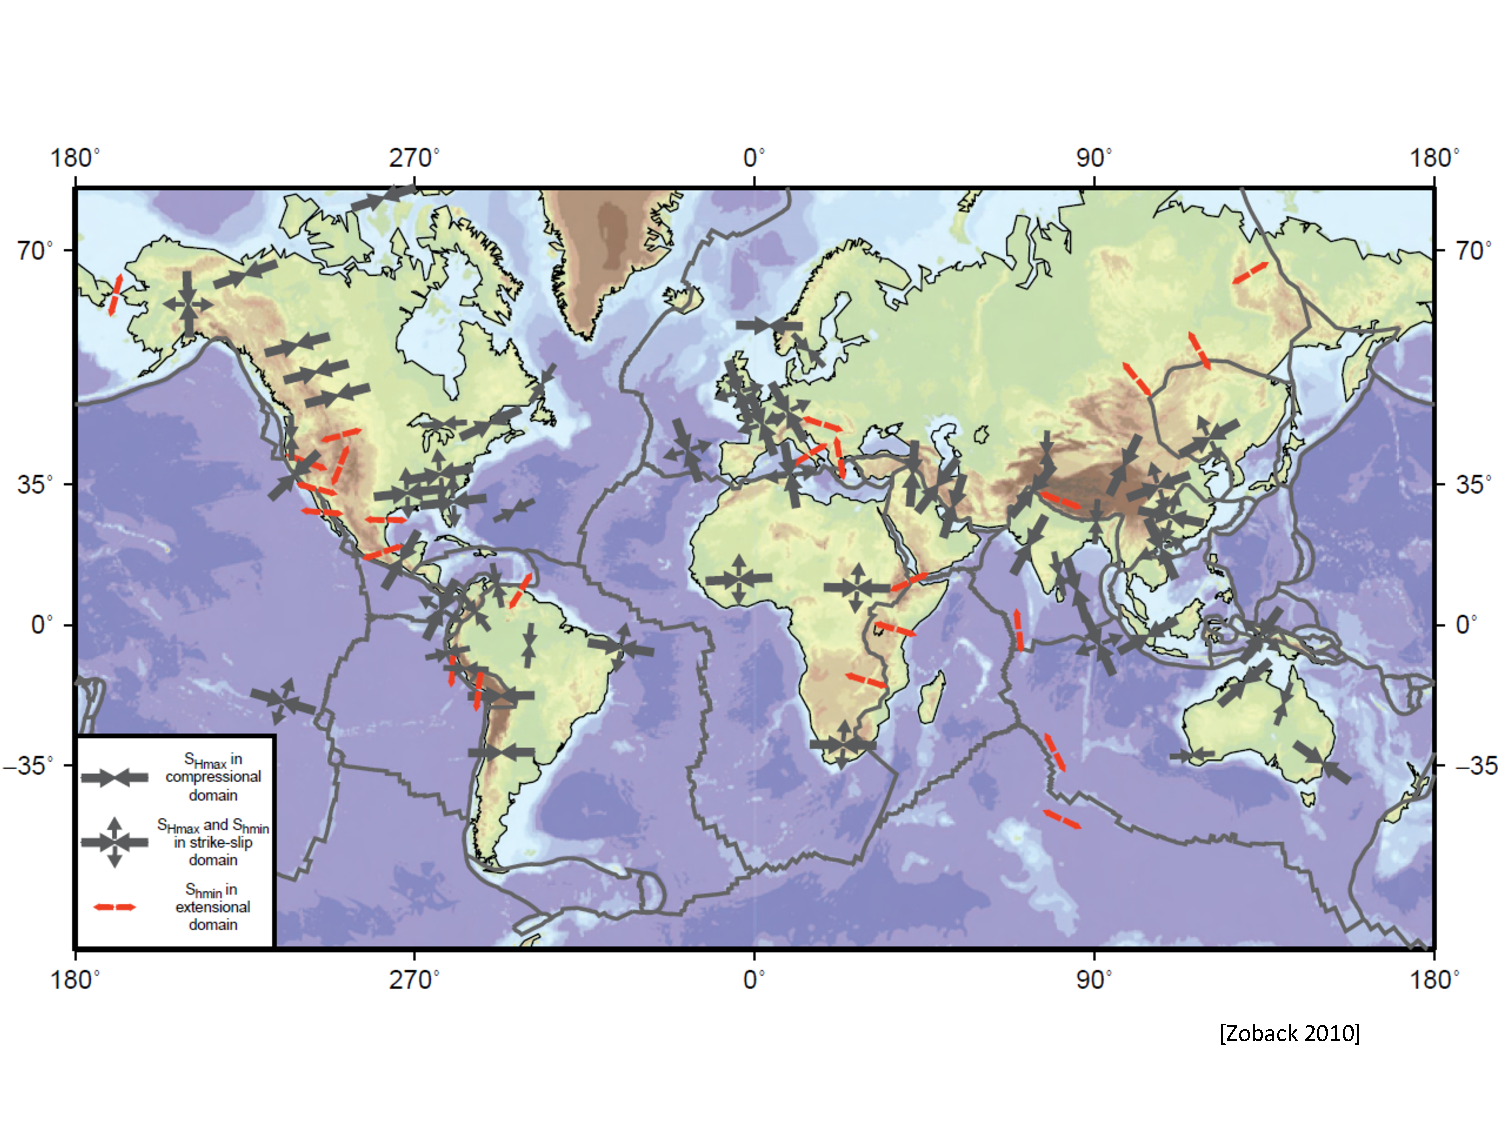
\includegraphics[scale=0.45]{.././Figures/split/1-2.pdf}%
\lthtmlpictureZ
\lthtmlcheckvsize\clearpage}

{\newpage\clearpage
\lthtmlpictureA{tex2html_wrap15050}%
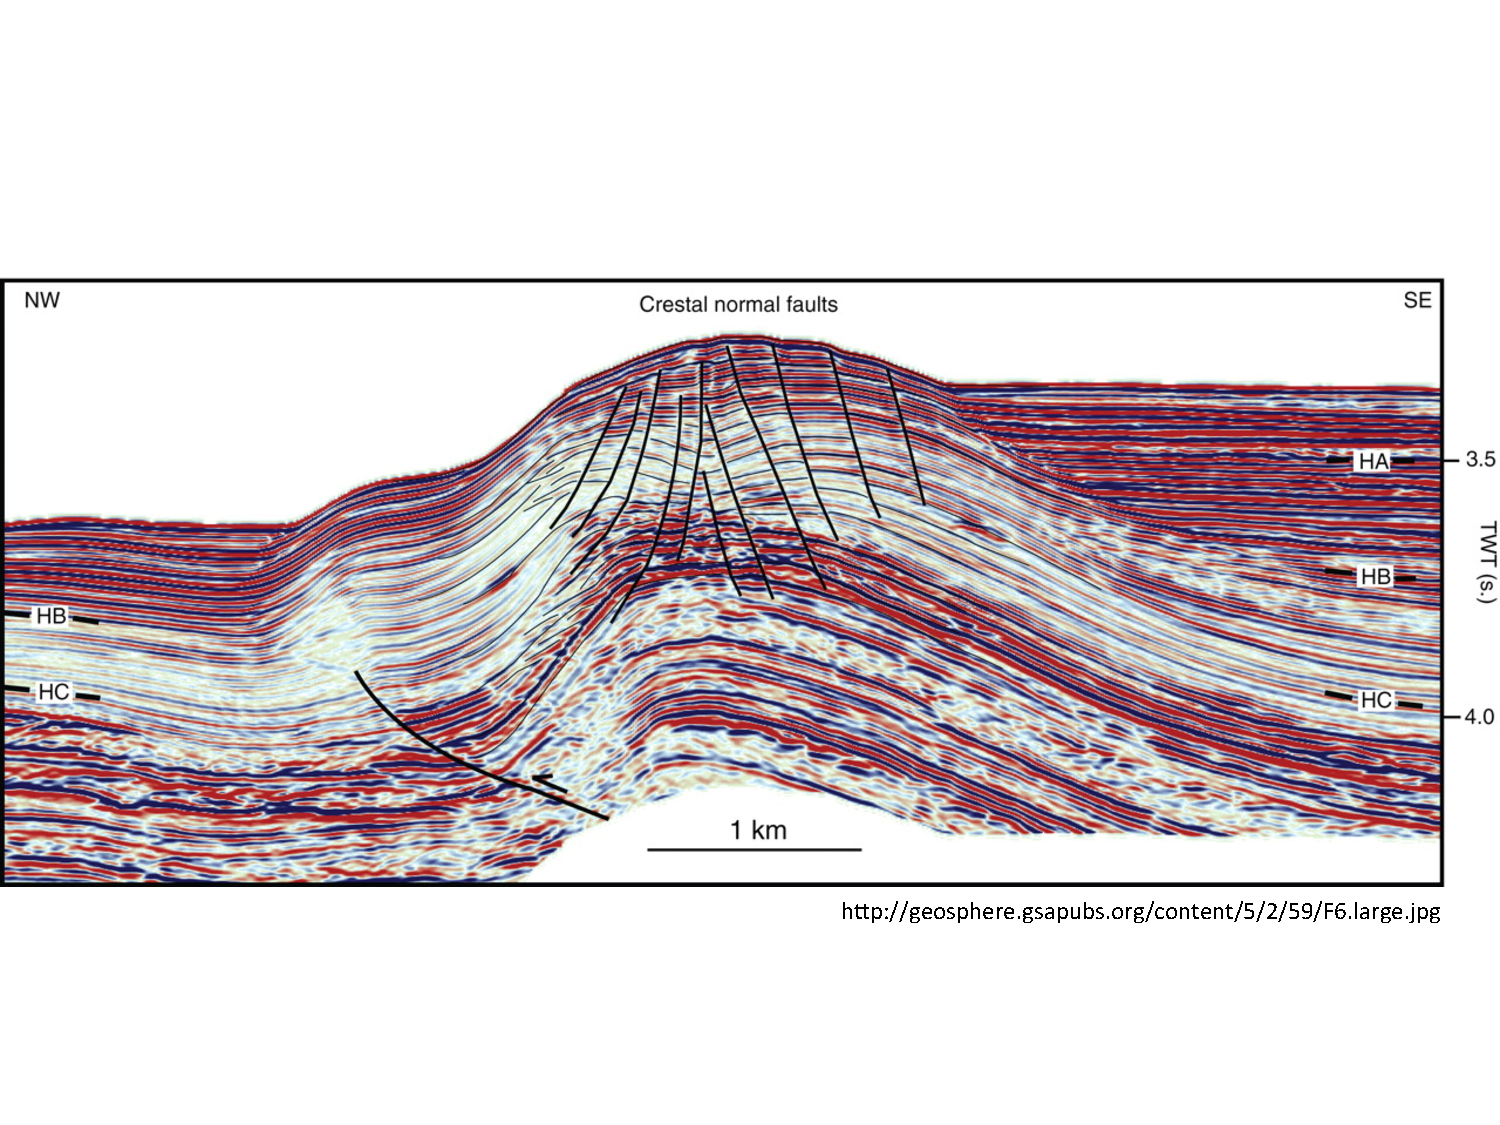
\includegraphics[scale=0.50]{.././Figures/split/1-3.pdf}%
\lthtmlpictureZ
\lthtmlcheckvsize\clearpage}

\stepcounter{section}
\stepcounter{subsection}
{\newpage\clearpage
\lthtmlpictureA{tex2html_wrap15059}%
\includegraphics[scale=0.55]{.././Figures/split/1-4.pdf}%
\lthtmlpictureZ
\lthtmlcheckvsize\clearpage}

\stepcounter{subsection}
{\newpage\clearpage
\lthtmlpictureA{tex2html_wrap15067}%
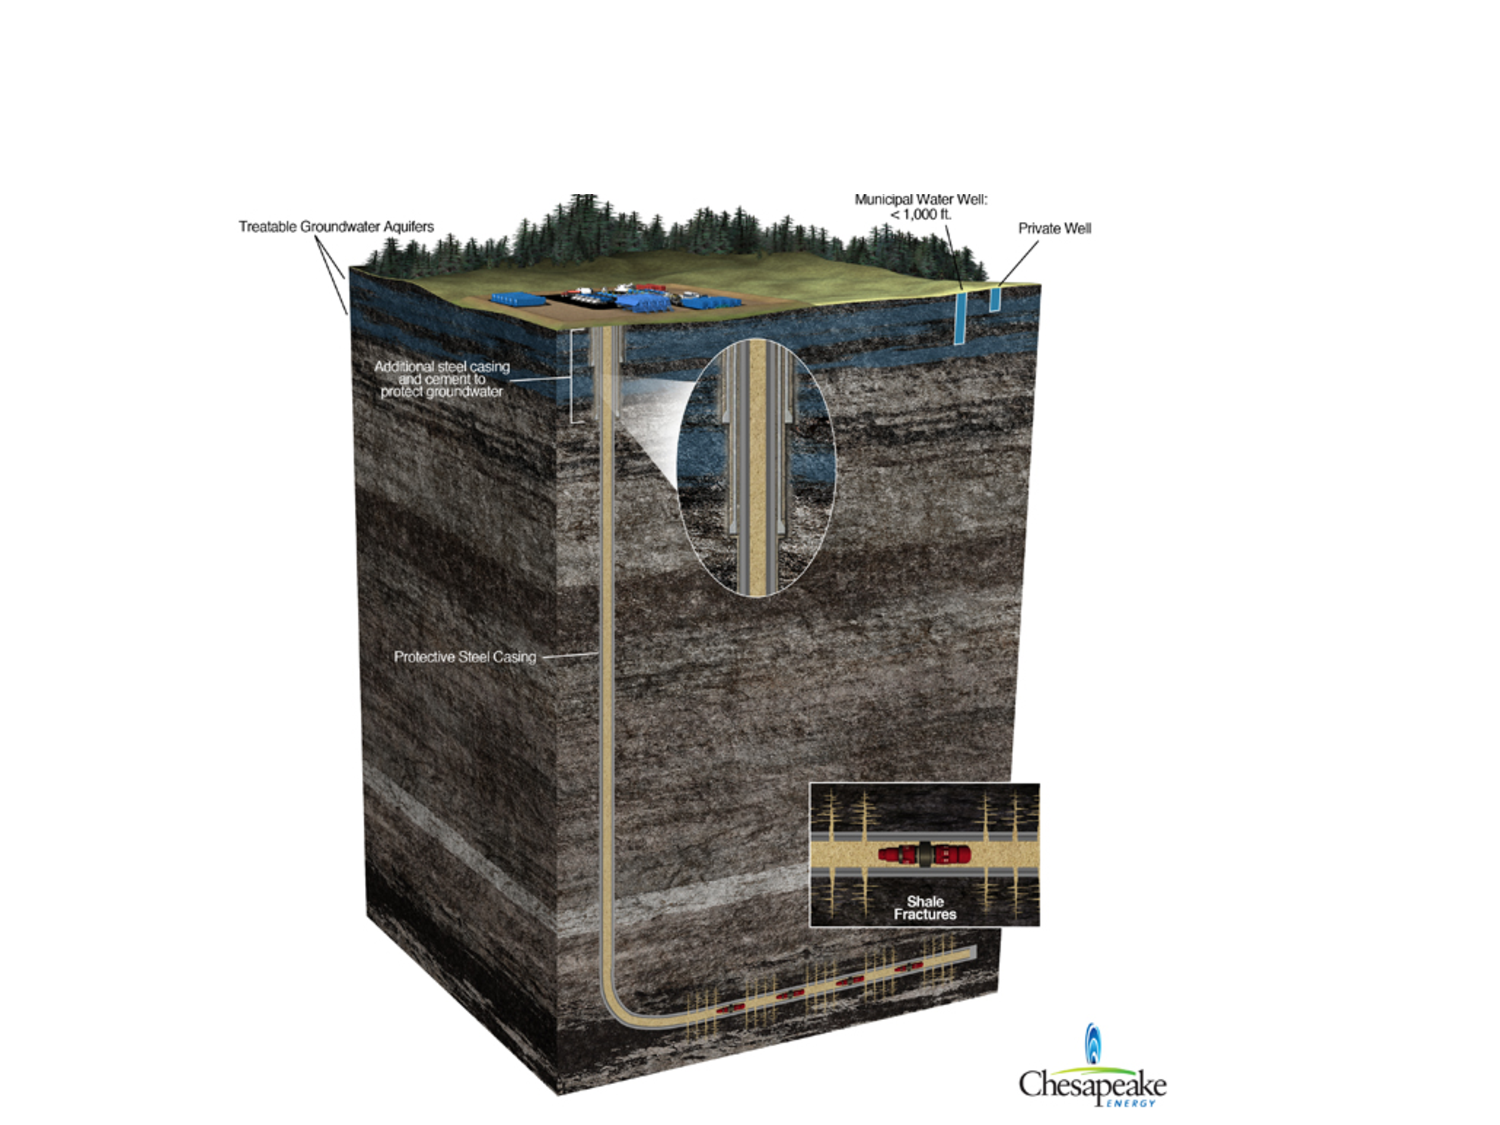
\includegraphics[scale=0.65]{.././Figures/split/1-6.pdf}%
\lthtmlpictureZ
\lthtmlcheckvsize\clearpage}

\stepcounter{subsection}
{\newpage\clearpage
\lthtmlpictureA{tex2html_wrap15073}%
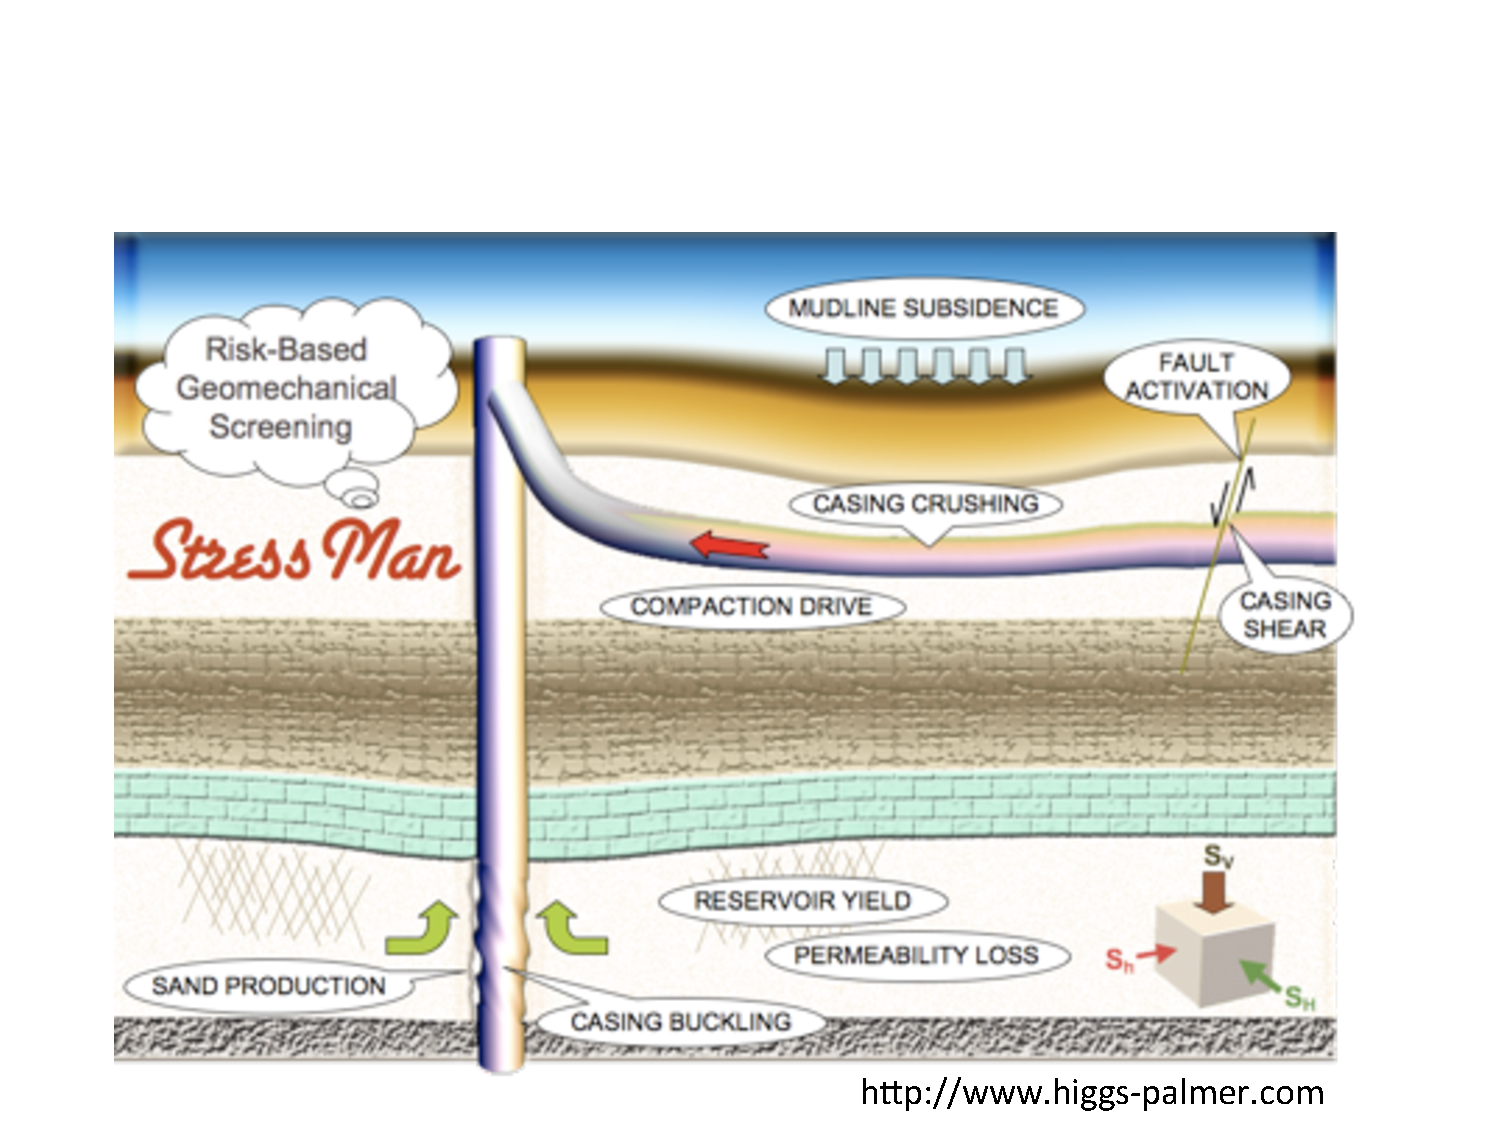
\includegraphics[scale=0.50]{.././Figures/split/1-5.pdf}%
\lthtmlpictureZ
\lthtmlcheckvsize\clearpage}

\stepcounter{section}
\stepcounter{chapter}
\stepcounter{section}
\stepcounter{subsection}
{\newpage\clearpage
\lthtmlinlinemathA{tex2html_wrap_inline15084}%
$ \uline{F}_1$%
\lthtmlindisplaymathZ
\lthtmlcheckvsize\clearpage}

{\newpage\clearpage
\lthtmlinlinemathA{tex2html_wrap_inline15086}%
$ \uline{F}_2$%
\lthtmlindisplaymathZ
\lthtmlcheckvsize\clearpage}

{\newpage\clearpage
\lthtmlinlinemathA{tex2html_wrap_inline15088}%
$ {\rm I\!R}^3$%
\lthtmlindisplaymathZ
\lthtmlcheckvsize\clearpage}

{\newpage\clearpage
\lthtmlinlinemathA{tex2html_wrap_inline15090}%
$ \uline{F}_1 = \uline{F}_2$%
\lthtmlindisplaymathZ
\lthtmlcheckvsize\clearpage}

{\newpage\clearpage
\lthtmlinlinemathA{tex2html_wrap_inline15092}%
$ \uline{F}_1 =  \uline{F}_2 + m \uline{g}$%
\lthtmlindisplaymathZ
\lthtmlcheckvsize\clearpage}

{\newpage\clearpage
\lthtmlinlinemathA{tex2html_wrap_inline15094}%
$ m \uline{g}$%
\lthtmlindisplaymathZ
\lthtmlcheckvsize\clearpage}

{\newpage\clearpage
\lthtmlinlinemathA{tex2html_wrap_inline15096}%
$ \uline{F}$%
\lthtmlindisplaymathZ
\lthtmlcheckvsize\clearpage}

{\newpage\clearpage
\lthtmlinlinemathA{tex2html_wrap_inline15098}%
$ A$%
\lthtmlindisplaymathZ
\lthtmlcheckvsize\clearpage}

{\newpage\clearpage
\lthtmlinlinemathA{tex2html_wrap_indisplay15100}%
$\displaystyle \uline{\sigma} = \frac{\uline{F}}{A}$%
\lthtmlindisplaymathZ
\lthtmlcheckvsize\clearpage}

{\newpage\clearpage
\lthtmlpictureA{tex2html_wrap15102}%
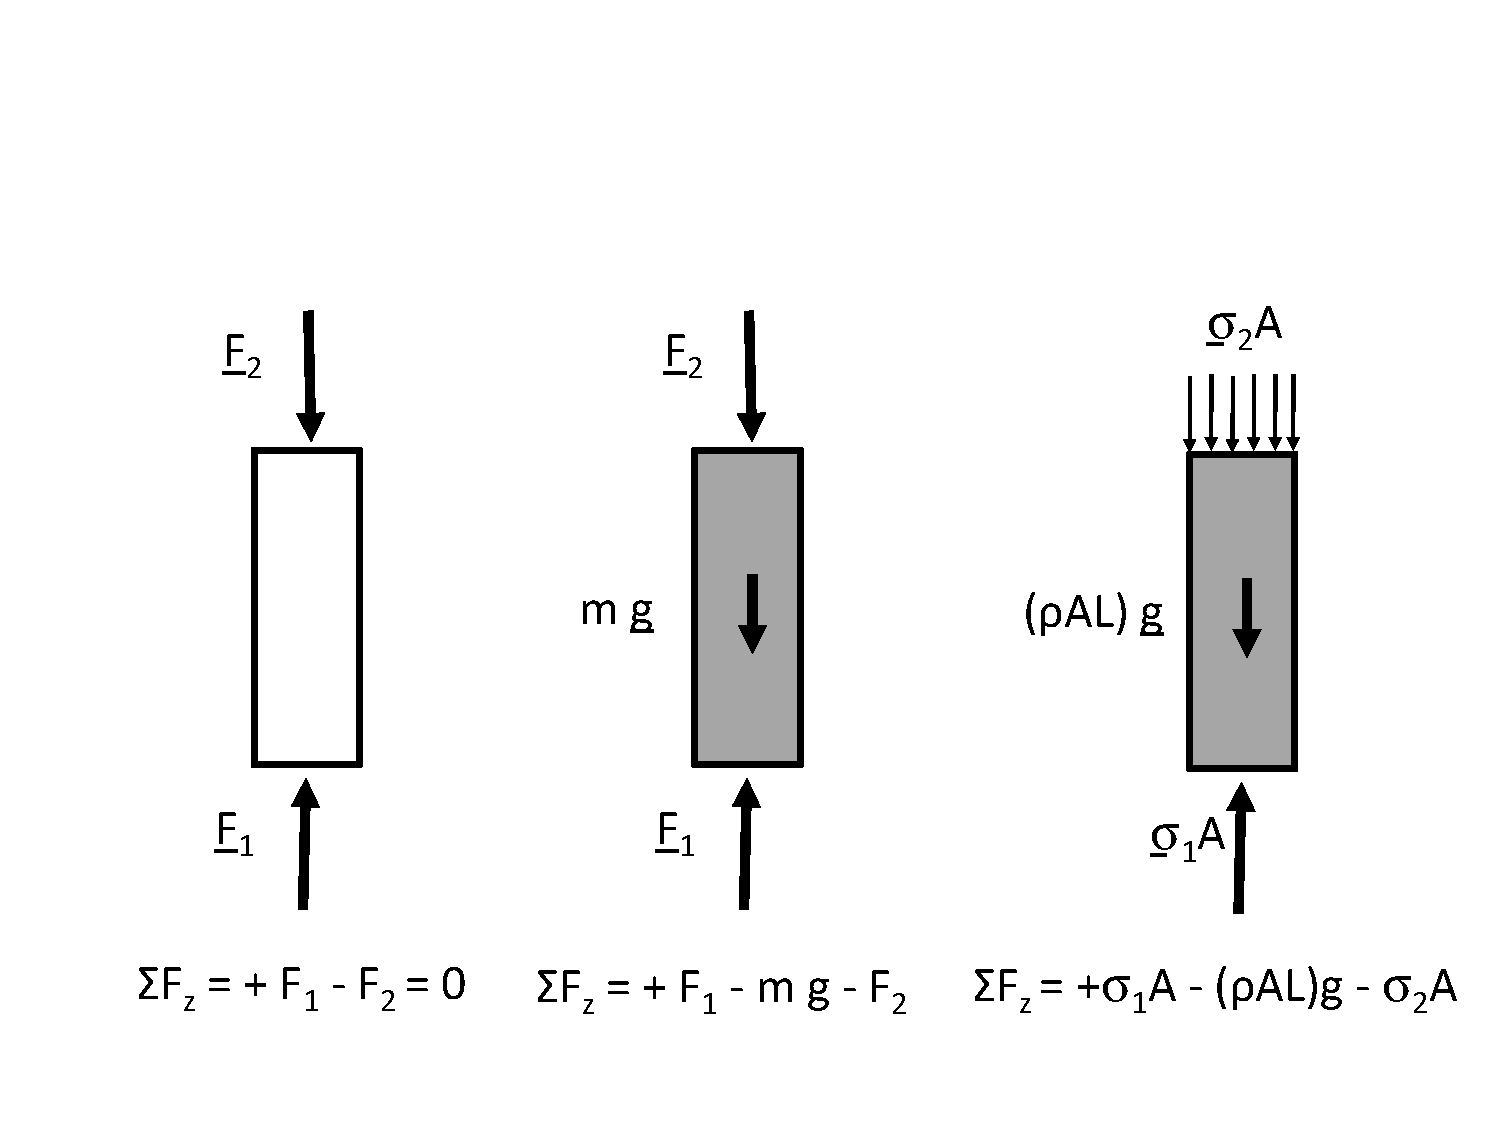
\includegraphics[scale=0.50]{.././Figures/split/2-2.pdf}%
\lthtmlpictureZ
\lthtmlcheckvsize\clearpage}

\stepcounter{subsection}
{\newpage\clearpage
\lthtmlinlinemathA{tex2html_wrap_inline15108}%
$ \Delta x \Delta y \Delta x$%
\lthtmlindisplaymathZ
\lthtmlcheckvsize\clearpage}

{\newpage\clearpage
\lthtmlinlinemathA{tex2html_wrap_inline15110}%
$ \sum \uline{F} = 0$%
\lthtmlindisplaymathZ
\lthtmlcheckvsize\clearpage}

{\newpage\clearpage
\lthtmlinlinemathA{tex2html_wrap_inline15112}%
$ \uline{g}$%
\lthtmlindisplaymathZ
\lthtmlcheckvsize\clearpage}

{\newpage\clearpage
\lthtmlinlinemathA{tex2html_wrap_inline15114}%
$ \sum F_z = 0$%
\lthtmlindisplaymathZ
\lthtmlcheckvsize\clearpage}

{\newpage\clearpage
\lthtmlinlinemathA{tex2html_wrap_indisplay15117}%
$\displaystyle S_v A + \rho_{bulk} Vol  g = S_v A + \Delta S_v A$%
\lthtmlindisplaymathZ
\lthtmlcheckvsize\clearpage}

{\newpage\clearpage
\lthtmlinlinemathA{tex2html_wrap_indisplay15119}%
$\displaystyle \rho_{bulk} \: \Delta x \Delta y \Delta z \:  g = \Delta S_v \Delta x \Delta y$%
\lthtmlindisplaymathZ
\lthtmlcheckvsize\clearpage}

{\newpage\clearpage
\lthtmlinlinemathA{tex2html_wrap_indisplay15121}%
$\displaystyle \frac{\Delta S_v}{\Delta z} = \rho_{bulk} \: g$%
\lthtmlindisplaymathZ
\lthtmlcheckvsize\clearpage}

{\newpage\clearpage
\lthtmlpictureA{tex2html_wrap15123}%
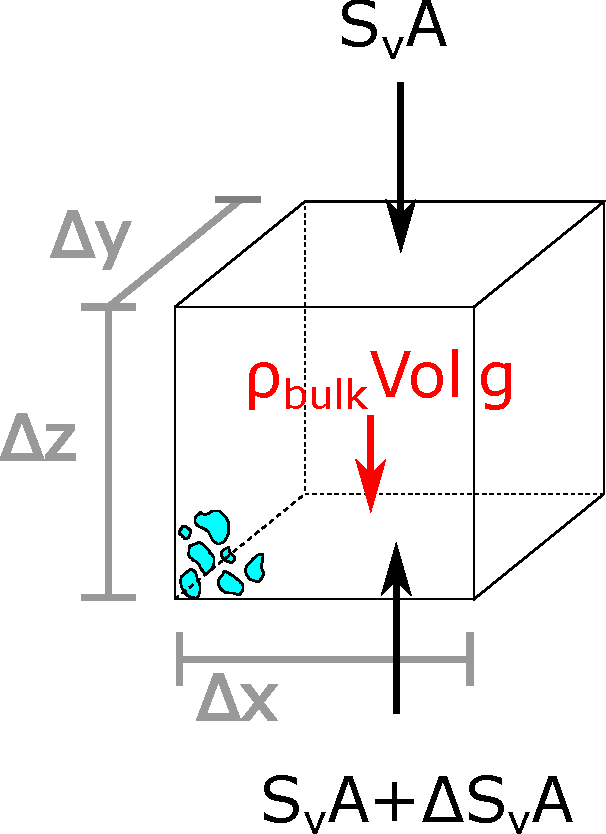
\includegraphics[scale=0.40]{.././Figures/split/2-REVoverburden.pdf}%
\lthtmlpictureZ
\lthtmlcheckvsize\clearpage}

{\newpage\clearpage
\lthtmlinlinemathA{tex2html_wrap_indisplay15128}%
$\displaystyle \int_0^{S_v(z)} dS_v = \int_0^z \rho_{bulk}(z) g \: dz$%
\lthtmlindisplaymathZ
\lthtmlcheckvsize\clearpage}

{\newpage\clearpage
\lthtmlinlinemathA{tex2html_wrap_inline15130}%
$ \rho_{bulk}(z) g$%
\lthtmlindisplaymathZ
\lthtmlcheckvsize\clearpage}

{\newpage\clearpage
\lthtmlinlinemathA{tex2html_wrap_inline15132}%
$ S_v(z=0)=0$%
\lthtmlindisplaymathZ
\lthtmlcheckvsize\clearpage}

{\newpage\clearpage
\lthtmlinlinemathA{tex2html_wrap_inline15134}%
$ \rho_{bulk} = cst$%
\lthtmlindisplaymathZ
\lthtmlcheckvsize\clearpage}

{\newpage\clearpage
\lthtmlinlinemathA{tex2html_wrap_inline15138}%
$ z$%
\lthtmlindisplaymathZ
\lthtmlcheckvsize\clearpage}

{\newpage\clearpage
\lthtmlinlinemathA{tex2html_wrap_indisplay15140}%
$\displaystyle S_v(z)  = \rho_{bulk} g \:z .$%
\lthtmlindisplaymathZ
\lthtmlcheckvsize\clearpage}

{\newpage\clearpage
\lthtmlinlinemathA{tex2html_wrap_inline15142}%
$ \rho_{SiO_2}$%
\lthtmlindisplaymathZ
\lthtmlcheckvsize\clearpage}

{\newpage\clearpage
\lthtmlinlinemathA{tex2html_wrap_inline15144}%
$ \rho_w$%
\lthtmlindisplaymathZ
\lthtmlcheckvsize\clearpage}

{\newpage\clearpage
\lthtmlinlinemathA{tex2html_wrap_inline15146}%
$ \rho_{bulk}$%
\lthtmlindisplaymathZ
\lthtmlcheckvsize\clearpage}

{\newpage\clearpage
\lthtmlinlinemathA{tex2html_wrap_inline15148}%
$ \phi$%
\lthtmlindisplaymathZ
\lthtmlcheckvsize\clearpage}

{\newpage\clearpage
\lthtmlinlinemathA{tex2html_wrap_indisplay15150}%
$\displaystyle \rho_{bulk} = (1-\phi) \rho_{SiO_2} + \phi \rho_w$%
\lthtmlindisplaymathZ
\lthtmlcheckvsize\clearpage}

{\newpage\clearpage
\lthtmlinlinemathA{tex2html_wrap_inline15152}%
$ \rho_{SiO_2} = 2650$%
\lthtmlindisplaymathZ
\lthtmlcheckvsize\clearpage}

{\newpage\clearpage
\lthtmlinlinemathA{tex2html_wrap_inline15154}%
$ ^3$%
\lthtmlindisplaymathZ
\lthtmlcheckvsize\clearpage}

{\newpage\clearpage
\lthtmlinlinemathA{tex2html_wrap_inline15156}%
$ \rho_w = 1000$%
\lthtmlindisplaymathZ
\lthtmlcheckvsize\clearpage}

{\newpage\clearpage
\lthtmlinlinemathA{tex2html_wrap_indisplay15160}%
$\displaystyle \rho_{bulk} = (1-0.2) 2650$%
\lthtmlindisplaymathZ
\lthtmlcheckvsize\clearpage}

{\newpage\clearpage
\lthtmlinlinemathA{tex2html_wrap_indisplay15161}%
$\displaystyle ^3 + (0.2) 1000$%
\lthtmlindisplaymathZ
\lthtmlcheckvsize\clearpage}

{\newpage\clearpage
\lthtmlinlinemathA{tex2html_wrap_indisplay15162}%
$\displaystyle ^3 = 2320$%
\lthtmlindisplaymathZ
\lthtmlcheckvsize\clearpage}

{\newpage\clearpage
\lthtmlinlinemathA{tex2html_wrap_indisplay15163}%
$\displaystyle ^3 .$%
\lthtmlindisplaymathZ
\lthtmlcheckvsize\clearpage}

{\newpage\clearpage
\lthtmlinlinemathA{tex2html_wrap_indisplay15167}%
$\displaystyle \rho_{bulk} g = 2320$%
\lthtmlindisplaymathZ
\lthtmlcheckvsize\clearpage}

{\newpage\clearpage
\lthtmlinlinemathA{tex2html_wrap_indisplay15168}%
$\displaystyle ^3 \: 9.8$%
\lthtmlindisplaymathZ
\lthtmlcheckvsize\clearpage}

{\newpage\clearpage
\lthtmlinlinemathA{tex2html_wrap_indisplay15169}%
$\displaystyle ^2 = 22.7 \times 10^3$%
\lthtmlindisplaymathZ
\lthtmlcheckvsize\clearpage}

{\newpage\clearpage
\lthtmlinlinemathA{tex2html_wrap_indisplay15170}%
$\displaystyle = 22.7$%
\lthtmlindisplaymathZ
\lthtmlcheckvsize\clearpage}

{\newpage\clearpage
\lthtmlinlinemathA{tex2html_wrap_indisplay15171}%
$\displaystyle . \: \: \blacksquare$%
\lthtmlindisplaymathZ
\lthtmlcheckvsize\clearpage}

{\newpage\clearpage
\lthtmlinlinemathA{tex2html_wrap_inline15173}%
$ \sim 1$%
\lthtmlindisplaymathZ
\lthtmlcheckvsize\clearpage}

{\newpage\clearpage
\lthtmlinlinemathA{tex2html_wrap_inline15175}%
$ \sim 23$%
\lthtmlindisplaymathZ
\lthtmlcheckvsize\clearpage}

{\newpage\clearpage
\lthtmlinlinemathA{tex2html_wrap_inline15177}%
$ \phi = 0.20$%
\lthtmlindisplaymathZ
\lthtmlcheckvsize\clearpage}

{\newpage\clearpage
\lthtmlinlinemathA{tex2html_wrap_inline15179}%
$ \sim 0.44$%
\lthtmlindisplaymathZ
\lthtmlcheckvsize\clearpage}

{\newpage\clearpage
\lthtmlinlinemathA{tex2html_wrap_inline15181}%
$ \sim 10$%
\lthtmlindisplaymathZ
\lthtmlcheckvsize\clearpage}

{\newpage\clearpage
\lthtmlinlinemathA{tex2html_wrap_inline15183}%
$ S_w, S_o, S_g$%
\lthtmlindisplaymathZ
\lthtmlcheckvsize\clearpage}

\stepcounter{subsubsection}
{\newpage\clearpage
\lthtmlinlinemathA{tex2html_wrap_indisplay15192}%
$\displaystyle P_p = \rho_w g \, z$%
\lthtmlindisplaymathZ
\lthtmlcheckvsize\clearpage}

{\newpage\clearpage
\lthtmlpictureA{tex2html_wrap15204}%
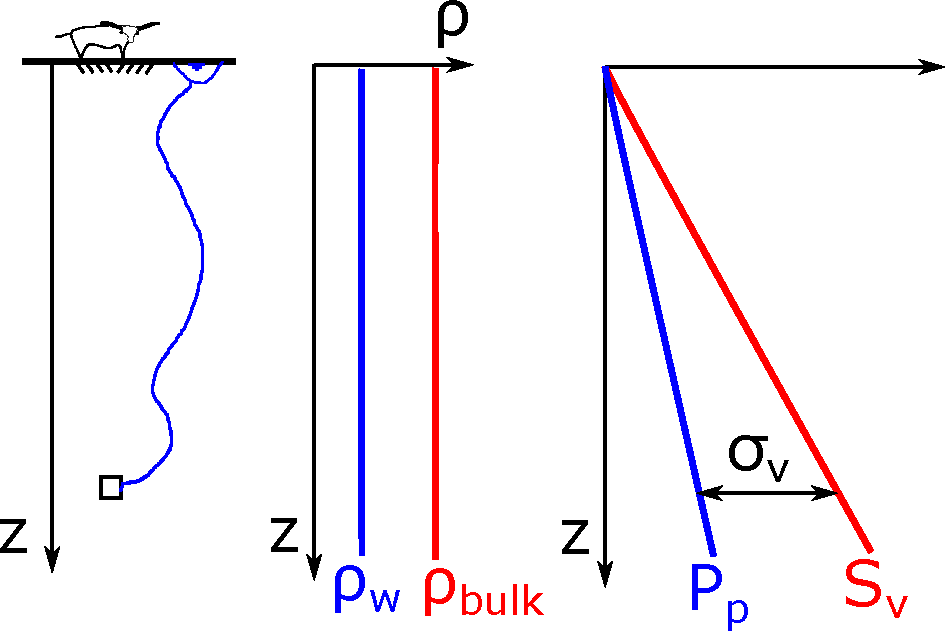
\includegraphics[scale=0.55]{.././Figures/split/2-OnshorePpSv.pdf}%
\lthtmlpictureZ
\lthtmlcheckvsize\clearpage}

{\newpage\clearpage
\lthtmlinlinemathA{tex2html_wrap_indisplay15221}%
$\displaystyle \sigma_v = S_v - P_p$%
\lthtmlindisplaymathZ
\lthtmlcheckvsize\clearpage}

{\newpage\clearpage
\lthtmlinlinemathA{tex2html_wrap_inline15223}%
$ S_v > P_p$%
\lthtmlindisplaymathZ
\lthtmlcheckvsize\clearpage}

{\newpage\clearpage
\lthtmlpictureA{tex2html_wrap15225}%
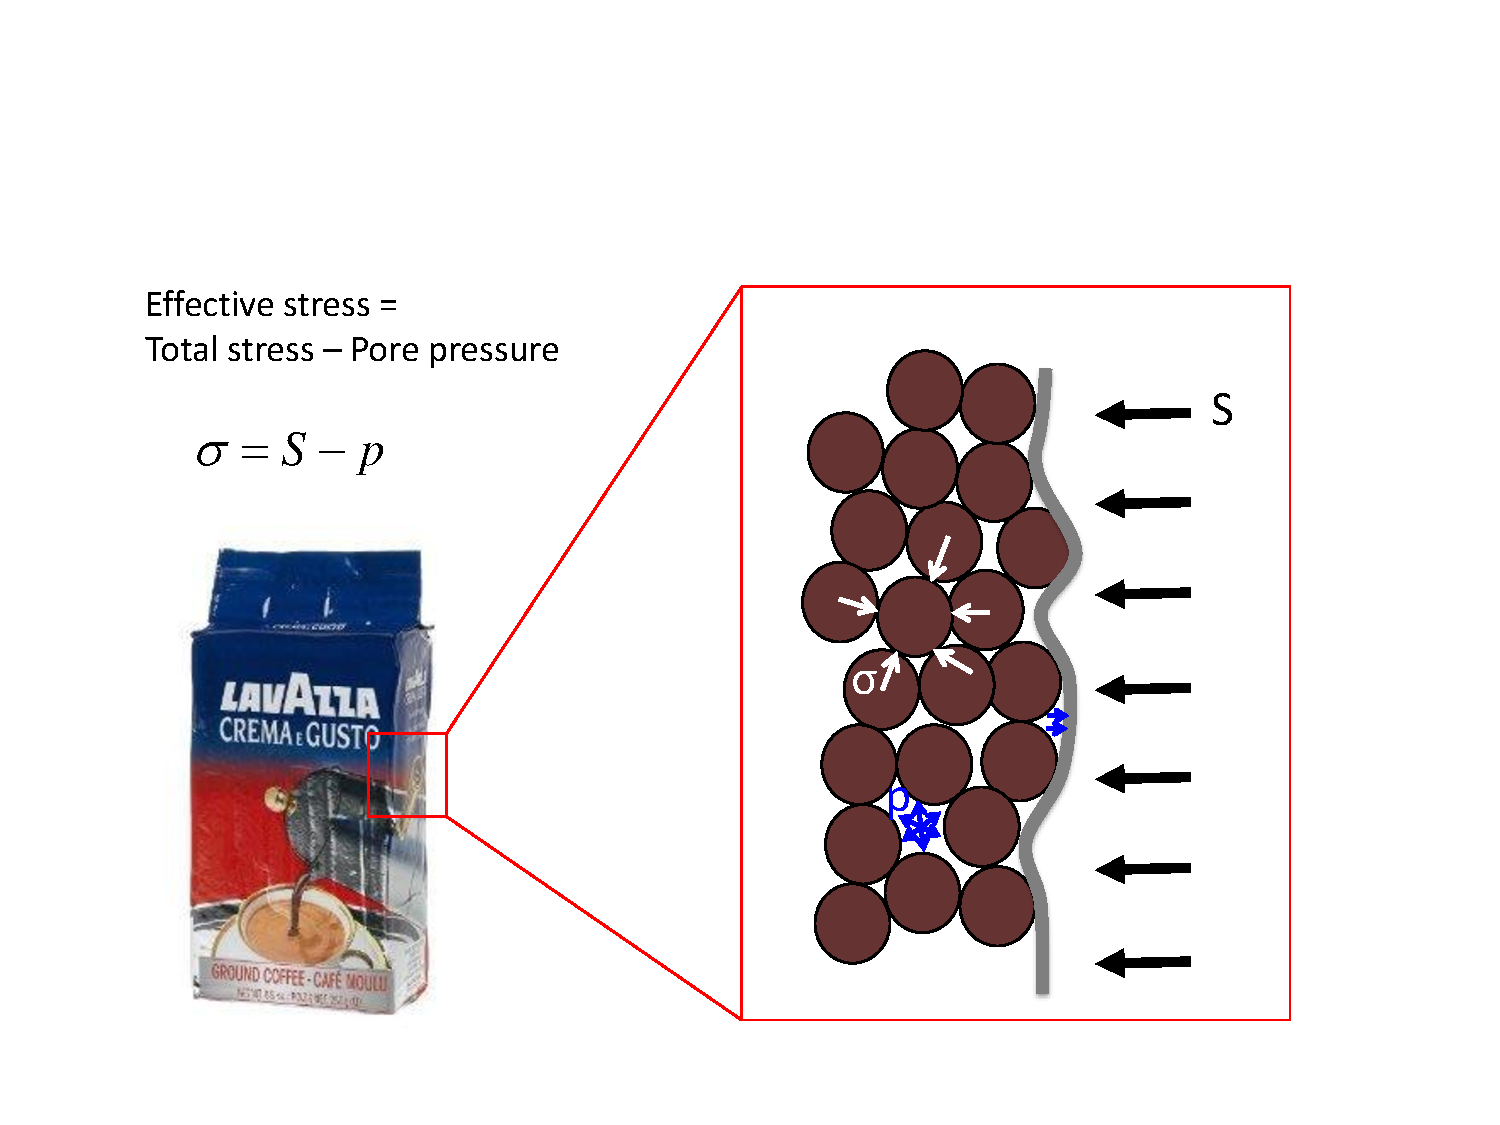
\includegraphics[scale=0.55]{.././Figures/split/2-20.pdf}%
\lthtmlpictureZ
\lthtmlcheckvsize\clearpage}

{\newpage\clearpage
\lthtmlinlinemathA{tex2html_wrap_inline15230}%
$ P_w$%
\lthtmlindisplaymathZ
\lthtmlcheckvsize\clearpage}

{\newpage\clearpage
\lthtmlinlinemathA{tex2html_wrap_indisplay15242}%
$\displaystyle \frac{dP_p}{dz} = \rho_w g = 1040$%
\lthtmlindisplaymathZ
\lthtmlcheckvsize\clearpage}

{\newpage\clearpage
\lthtmlinlinemathA{tex2html_wrap_indisplay15243}%
$\displaystyle ^3 \times 9.8$%
\lthtmlindisplaymathZ
\lthtmlcheckvsize\clearpage}

{\newpage\clearpage
\lthtmlinlinemathA{tex2html_wrap_indisplay15244}%
$\displaystyle ^2 = 10.19$%
\lthtmlindisplaymathZ
\lthtmlcheckvsize\clearpage}

{\newpage\clearpage
\lthtmlinlinemathA{tex2html_wrap_indisplay15246}%
$\displaystyle \frac{dS_v}{dz} = \rho_{bulk} g = 2350$%
\lthtmlindisplaymathZ
\lthtmlcheckvsize\clearpage}

{\newpage\clearpage
\lthtmlinlinemathA{tex2html_wrap_indisplay15248}%
$\displaystyle ^2 = 23.03$%
\lthtmlindisplaymathZ
\lthtmlcheckvsize\clearpage}

{\newpage\clearpage
\lthtmlinlinemathA{tex2html_wrap_indisplay15250}%
$\displaystyle P_p = \frac{dP_p}{dz} z = 10.19$%
\lthtmlindisplaymathZ
\lthtmlcheckvsize\clearpage}

{\newpage\clearpage
\lthtmlinlinemathA{tex2html_wrap_indisplay15251}%
$\displaystyle \times 1.219$%
\lthtmlindisplaymathZ
\lthtmlcheckvsize\clearpage}

{\newpage\clearpage
\lthtmlinlinemathA{tex2html_wrap_indisplay15252}%
$\displaystyle =  12.43$%
\lthtmlindisplaymathZ
\lthtmlcheckvsize\clearpage}

{\newpage\clearpage
\lthtmlinlinemathA{tex2html_wrap_indisplay15253}%
$\displaystyle = 1801$%
\lthtmlindisplaymathZ
\lthtmlcheckvsize\clearpage}

{\newpage\clearpage
\lthtmlinlinemathA{tex2html_wrap_indisplay15255}%
$\displaystyle \frac{dS_v}{dz} z = 23.03$%
\lthtmlindisplaymathZ
\lthtmlcheckvsize\clearpage}

{\newpage\clearpage
\lthtmlinlinemathA{tex2html_wrap_indisplay15257}%
$\displaystyle =  28.07$%
\lthtmlindisplaymathZ
\lthtmlcheckvsize\clearpage}

{\newpage\clearpage
\lthtmlinlinemathA{tex2html_wrap_indisplay15258}%
$\displaystyle = 4070$%
\lthtmlindisplaymathZ
\lthtmlcheckvsize\clearpage}

\stepcounter{subsubsection}
{\newpage\clearpage
\lthtmlinlinemathA{tex2html_wrap_inline15262}%
$ z_w$%
\lthtmlindisplaymathZ
\lthtmlcheckvsize\clearpage}

{\newpage\clearpage
\lthtmlinlinemathA{tex2html_wrap_inline15266}%
$ z > z_w$%
\lthtmlindisplaymathZ
\lthtmlcheckvsize\clearpage}

{\newpage\clearpage
\lthtmlinlinemathA{tex2html_wrap_indisplay15268}%
$\displaystyle S_v = \rho_{w} g \, z_w + \rho_{bulk} g (z-z_w)$%
\lthtmlindisplaymathZ
\lthtmlcheckvsize\clearpage}

{\newpage\clearpage
\lthtmlinlinemathA{tex2html_wrap_indisplay15269}%
$\displaystyle \quad z \geq z_w$%
\lthtmlindisplaymathZ
\lthtmlcheckvsize\clearpage}

{\newpage\clearpage
\lthtmlpictureA{tex2html_wrap15271}%
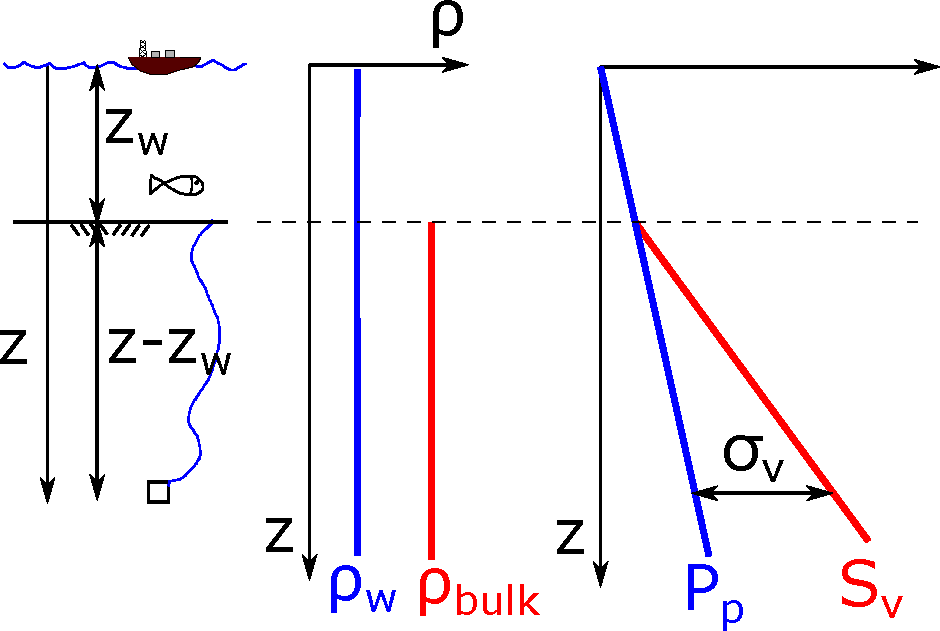
\includegraphics[scale=0.55]{.././Figures/split/2-OffshorePpSv.pdf}%
\lthtmlpictureZ
\lthtmlcheckvsize\clearpage}

{\newpage\clearpage
\lthtmlinlinemathA{tex2html_wrap_inline15276}%
$ z=z_w$%
\lthtmlindisplaymathZ
\lthtmlcheckvsize\clearpage}

{\newpage\clearpage
\lthtmlinlinemathA{tex2html_wrap_indisplay15278}%
$\displaystyle \sigma_v = S_v - P_p =  \rho_{bulk} g (z-z_w)$%
\lthtmlindisplaymathZ
\lthtmlcheckvsize\clearpage}

{\newpage\clearpage
\lthtmlinlinemathA{tex2html_wrap_indisplay15285}%
$\displaystyle P_p = \rho_w g z_w + \frac{dP_p}{dz} (z-z_w)  = 0.44$%
\lthtmlindisplaymathZ
\lthtmlcheckvsize\clearpage}

{\newpage\clearpage
\lthtmlinlinemathA{tex2html_wrap_indisplay15286}%
$\displaystyle \times 2000$%
\lthtmlindisplaymathZ
\lthtmlcheckvsize\clearpage}

{\newpage\clearpage
\lthtmlinlinemathA{tex2html_wrap_indisplay15287}%
$\displaystyle + 0.44$%
\lthtmlindisplaymathZ
\lthtmlcheckvsize\clearpage}

{\newpage\clearpage
\lthtmlinlinemathA{tex2html_wrap_indisplay15288}%
$\displaystyle \times (9000-2000)$%
\lthtmlindisplaymathZ
\lthtmlcheckvsize\clearpage}

{\newpage\clearpage
\lthtmlinlinemathA{tex2html_wrap_indisplay15289}%
$\displaystyle =   3960$%
\lthtmlindisplaymathZ
\lthtmlcheckvsize\clearpage}

{\newpage\clearpage
\lthtmlinlinemathA{tex2html_wrap_indisplay15291}%
$\displaystyle S_v = \rho_w g z_w + \frac{dS_v}{dz} (z-z_w)  = 0.44$%
\lthtmlindisplaymathZ
\lthtmlcheckvsize\clearpage}

{\newpage\clearpage
\lthtmlinlinemathA{tex2html_wrap_indisplay15293}%
$\displaystyle + 1.00$%
\lthtmlindisplaymathZ
\lthtmlcheckvsize\clearpage}

{\newpage\clearpage
\lthtmlinlinemathA{tex2html_wrap_indisplay15295}%
$\displaystyle = 7880$%
\lthtmlindisplaymathZ
\lthtmlcheckvsize\clearpage}

{\newpage\clearpage
\lthtmlinlinemathA{tex2html_wrap_indisplay15296}%
$\displaystyle ,$%
\lthtmlindisplaymathZ
\lthtmlcheckvsize\clearpage}

{\newpage\clearpage
\lthtmlinlinemathA{tex2html_wrap_indisplay15298}%
$\displaystyle \sigma_v = S_v - P_p = 7880$%
\lthtmlindisplaymathZ
\lthtmlcheckvsize\clearpage}

{\newpage\clearpage
\lthtmlinlinemathA{tex2html_wrap_indisplay15299}%
$\displaystyle - 3960$%
\lthtmlindisplaymathZ
\lthtmlcheckvsize\clearpage}

{\newpage\clearpage
\lthtmlinlinemathA{tex2html_wrap_indisplay15300}%
$\displaystyle = 3920$%
\lthtmlindisplaymathZ
\lthtmlcheckvsize\clearpage}

{\newpage\clearpage
\lthtmlinlinemathA{tex2html_wrap_indisplay15301}%
$\displaystyle .$%
\lthtmlindisplaymathZ
\lthtmlcheckvsize\clearpage}

{\newpage\clearpage
\lthtmlinlinemathA{tex2html_wrap_inline15303}%
$ P_p = 27.31$%
\lthtmlindisplaymathZ
\lthtmlcheckvsize\clearpage}

{\newpage\clearpage
\lthtmlinlinemathA{tex2html_wrap_inline15305}%
$ S_v =  54.34$%
\lthtmlindisplaymathZ
\lthtmlcheckvsize\clearpage}

{\newpage\clearpage
\lthtmlinlinemathA{tex2html_wrap_inline15307}%
$ \sigma_v = 27.03$%
\lthtmlindisplaymathZ
\lthtmlcheckvsize\clearpage}

{\newpage\clearpage
\lthtmlinlinemathA{tex2html_wrap_inline15309}%
$ \: \: \blacksquare$%
\lthtmlindisplaymathZ
\lthtmlcheckvsize\clearpage}

\stepcounter{subsubsection}
{\newpage\clearpage
\lthtmlinlinemathA{tex2html_wrap_indisplay15314}%
$\displaystyle S_v(z) = \int_0^z \rho_{bulk}(z) g \: dz$%
\lthtmlindisplaymathZ
\lthtmlcheckvsize\clearpage}

{\newpage\clearpage
\lthtmlinlinemathA{tex2html_wrap_inline15316}%
$ \rho_{bulk}(z)$%
\lthtmlindisplaymathZ
\lthtmlcheckvsize\clearpage}

{\newpage\clearpage
\lthtmlinlinemathA{tex2html_wrap_indisplay15324}%
$\displaystyle S_v(z_i) = \sum\limits_1^i \rho_{bulk}(z_i) g \Delta z_i$%
\lthtmlindisplaymathZ
\lthtmlcheckvsize\clearpage}

{\newpage\clearpage
\lthtmlinlinemathA{tex2html_wrap_inline15326}%
$ i$%
\lthtmlindisplaymathZ
\lthtmlcheckvsize\clearpage}

{\newpage\clearpage
\lthtmlinlinemathA{tex2html_wrap_inline15328}%
$ z_i$%
\lthtmlindisplaymathZ
\lthtmlcheckvsize\clearpage}

{\newpage\clearpage
\lthtmlpictureA{tex2html_wrap15332}%
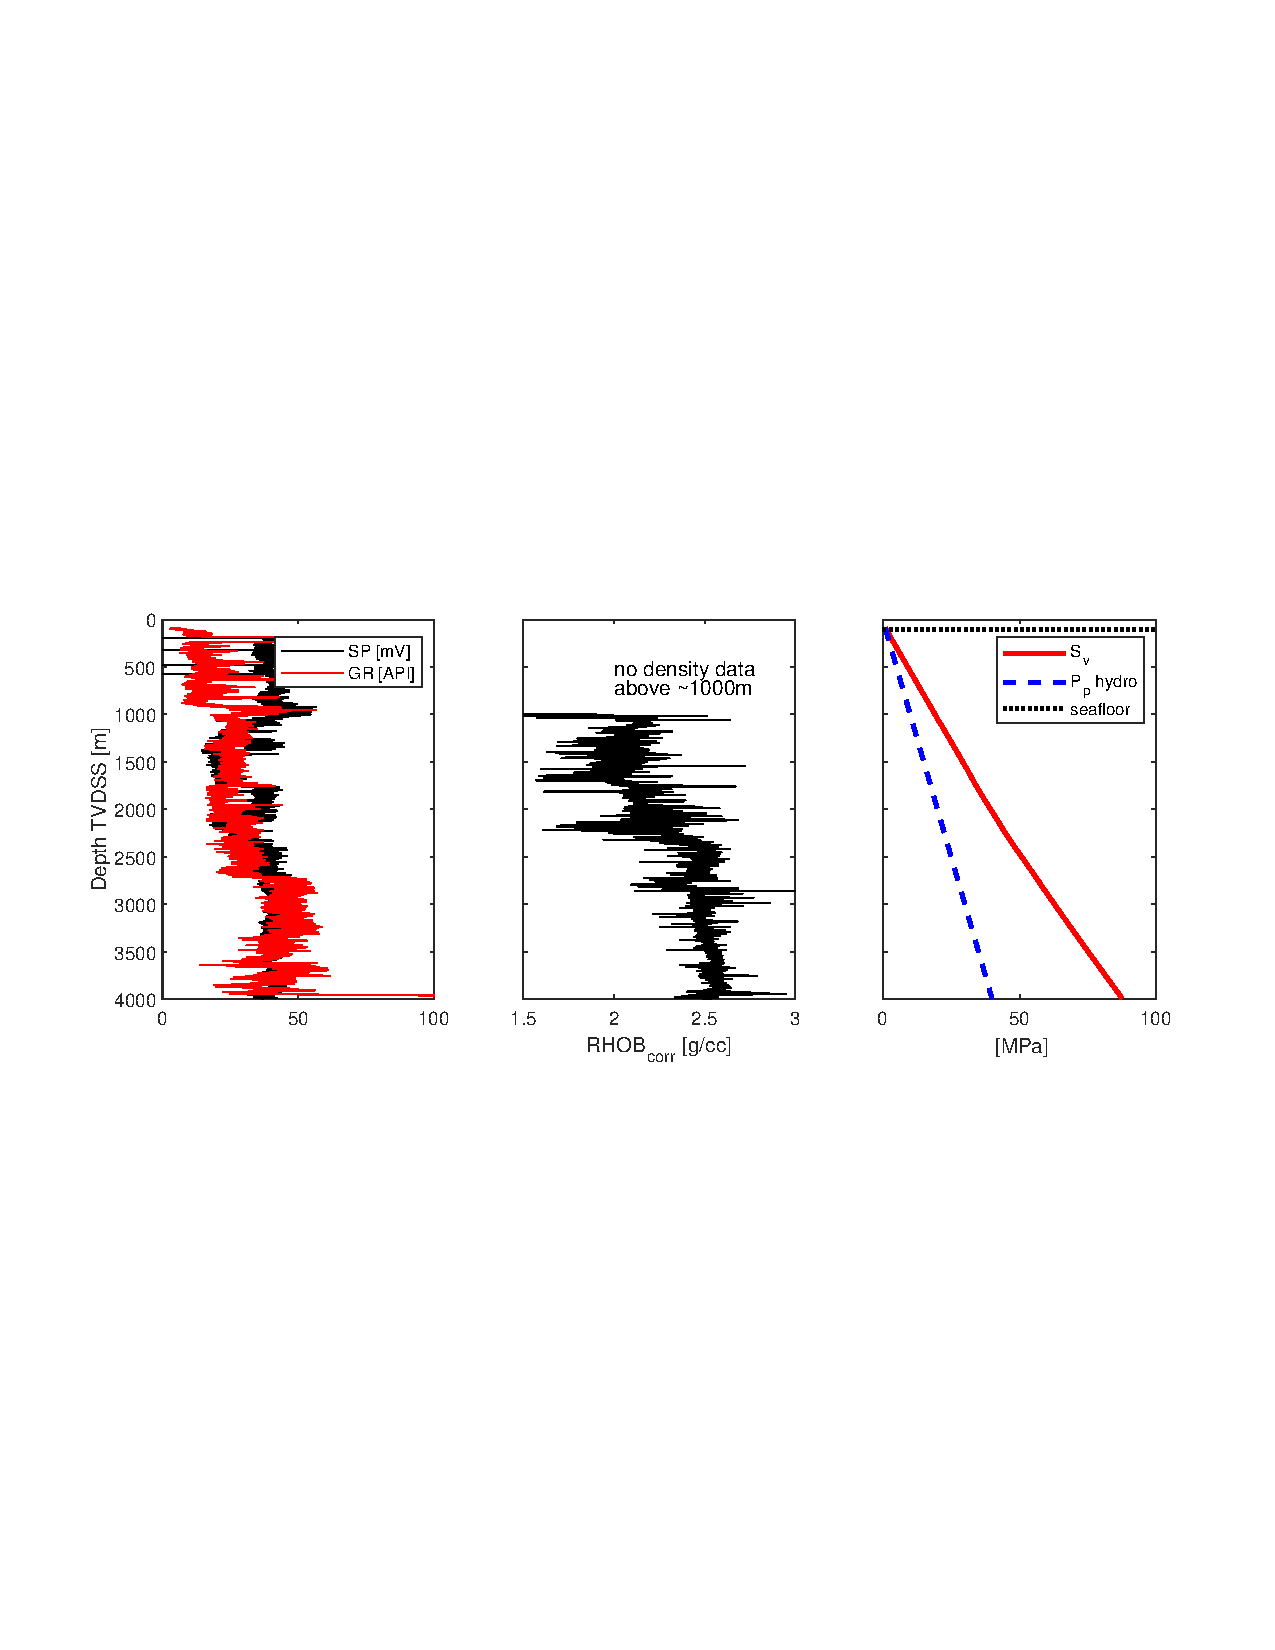
\includegraphics[scale=0.85]{.././Figures/split/2-VertStress_TVDSS.pdf}%
\lthtmlpictureZ
\lthtmlcheckvsize\clearpage}

\stepcounter{section}
{\newpage\clearpage
\lthtmlinlinemathA{tex2html_wrap_inline15338}%
$ z \sim 8,500$%
\lthtmlindisplaymathZ
\lthtmlcheckvsize\clearpage}

{\newpage\clearpage
\lthtmlinlinemathA{tex2html_wrap_inline15342}%
$ z \sim 11,000$%
\lthtmlindisplaymathZ
\lthtmlcheckvsize\clearpage}

{\newpage\clearpage
\lthtmlpictureA{tex2html_wrap15346}%
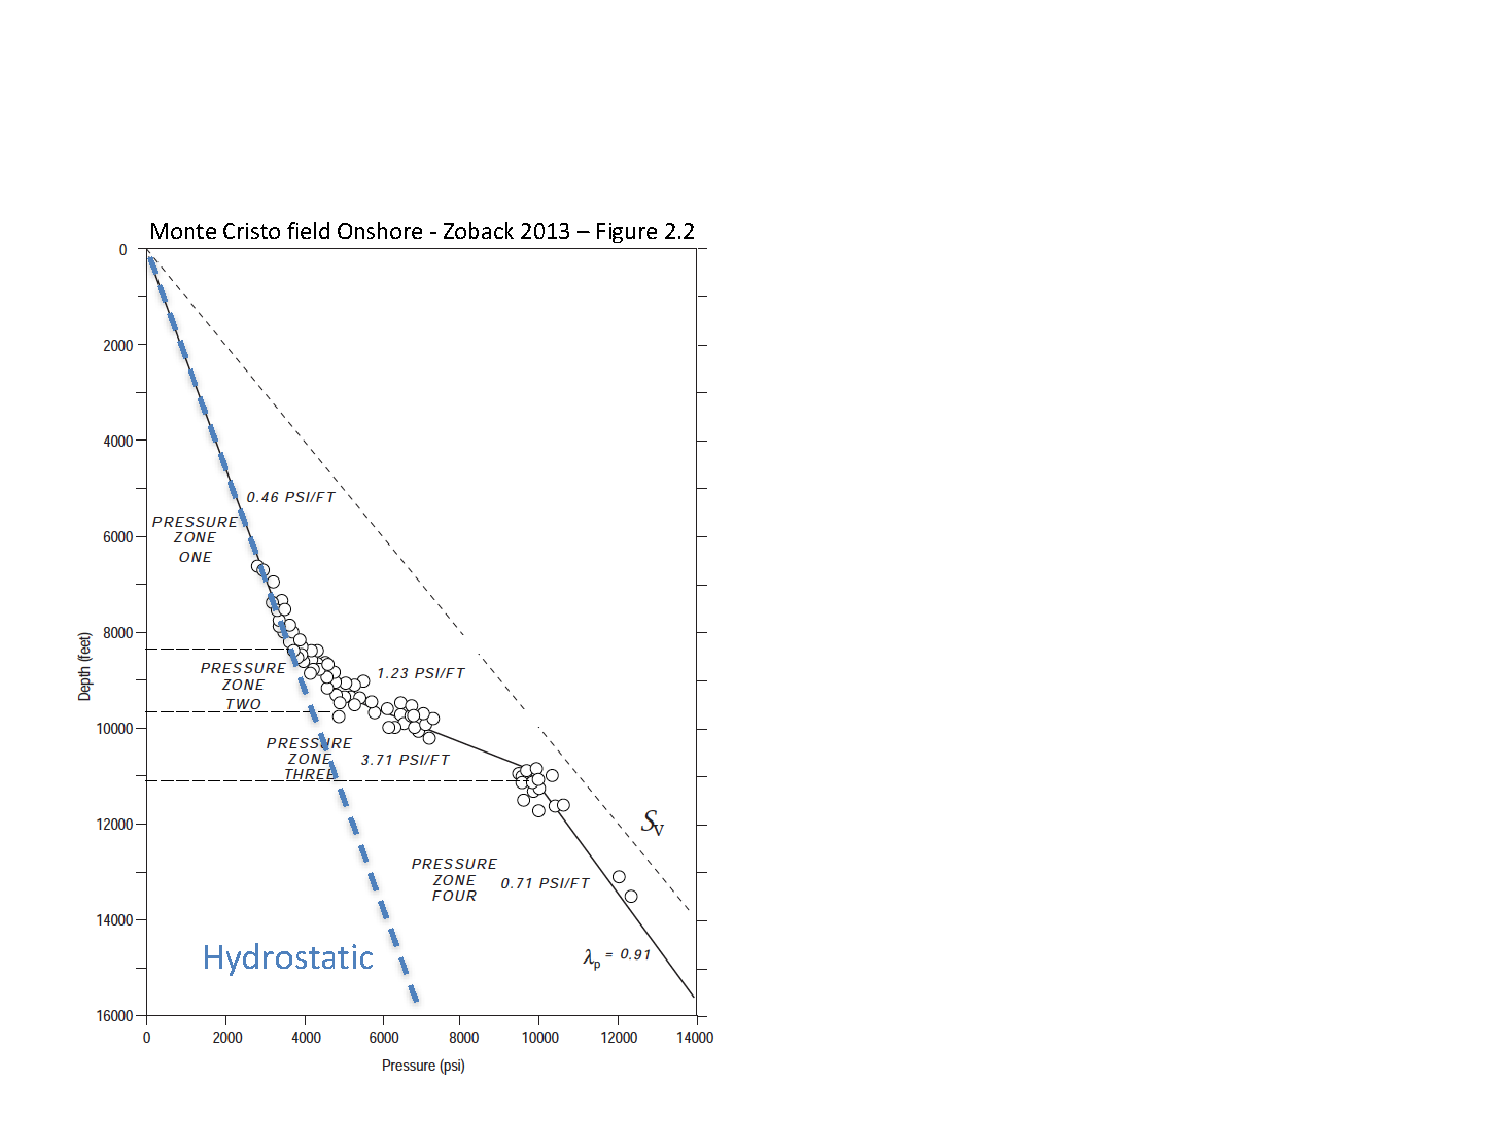
\includegraphics[scale=0.65]{.././Figures/split/2-9.pdf}%
\lthtmlpictureZ
\lthtmlcheckvsize\clearpage}

{\newpage\clearpage
\lthtmlinlinemathA{tex2html_wrap_inline15351}%
$ \lambda_p$%
\lthtmlindisplaymathZ
\lthtmlcheckvsize\clearpage}

{\newpage\clearpage
\lthtmlinlinemathA{tex2html_wrap_indisplay15353}%
$\displaystyle \lambda_p(z) = \frac{P_p(z)}{S_v(z)}$%
\lthtmlindisplaymathZ
\lthtmlcheckvsize\clearpage}

{\newpage\clearpage
\lthtmlinlinemathA{tex2html_wrap_inline15359}%
$ \lambda_p \leq 1$%
\lthtmlindisplaymathZ
\lthtmlcheckvsize\clearpage}

{\newpage\clearpage
\lthtmlinlinemathA{tex2html_wrap_inline15361}%
$ \lambda_p \sim 0.44$%
\lthtmlindisplaymathZ
\lthtmlcheckvsize\clearpage}

{\newpage\clearpage
\lthtmlinlinemathA{tex2html_wrap_inline15363}%
$ \lambda_p \neq 0.44$%
\lthtmlindisplaymathZ
\lthtmlcheckvsize\clearpage}

{\newpage\clearpage
\lthtmlinlinemathA{tex2html_wrap_inline15365}%
$ \lambda_p \rightarrow 1$%
\lthtmlindisplaymathZ
\lthtmlcheckvsize\clearpage}

\stepcounter{subsection}
{\newpage\clearpage
\lthtmlinlinemathA{tex2html_wrap_inline15368}%
$ P_p > P_p^{\text{hydrostatic}}$%
\lthtmlindisplaymathZ
\lthtmlcheckvsize\clearpage}

{\newpage\clearpage
\lthtmlinlinemathA{tex2html_wrap_inline15370}%
$ \Delta P_p$%
\lthtmlindisplaymathZ
\lthtmlcheckvsize\clearpage}

{\newpage\clearpage
\lthtmlinlinemathA{tex2html_wrap_inline15372}%
$ h$%
\lthtmlindisplaymathZ
\lthtmlcheckvsize\clearpage}

{\newpage\clearpage
\lthtmlinlinemathA{tex2html_wrap_inline15374}%
$ \rho_{brine} - \rho_{hydrocarbon}$%
\lthtmlindisplaymathZ
\lthtmlcheckvsize\clearpage}

{\newpage\clearpage
\lthtmlinlinemathA{tex2html_wrap_indisplay15376}%
$\displaystyle \Delta P = (\rho_{brine} - \rho_{hydrocarbon}) g  h$%
\lthtmlindisplaymathZ
\lthtmlcheckvsize\clearpage}

{\newpage\clearpage
\lthtmlpictureA{tex2html_wrap15384}%
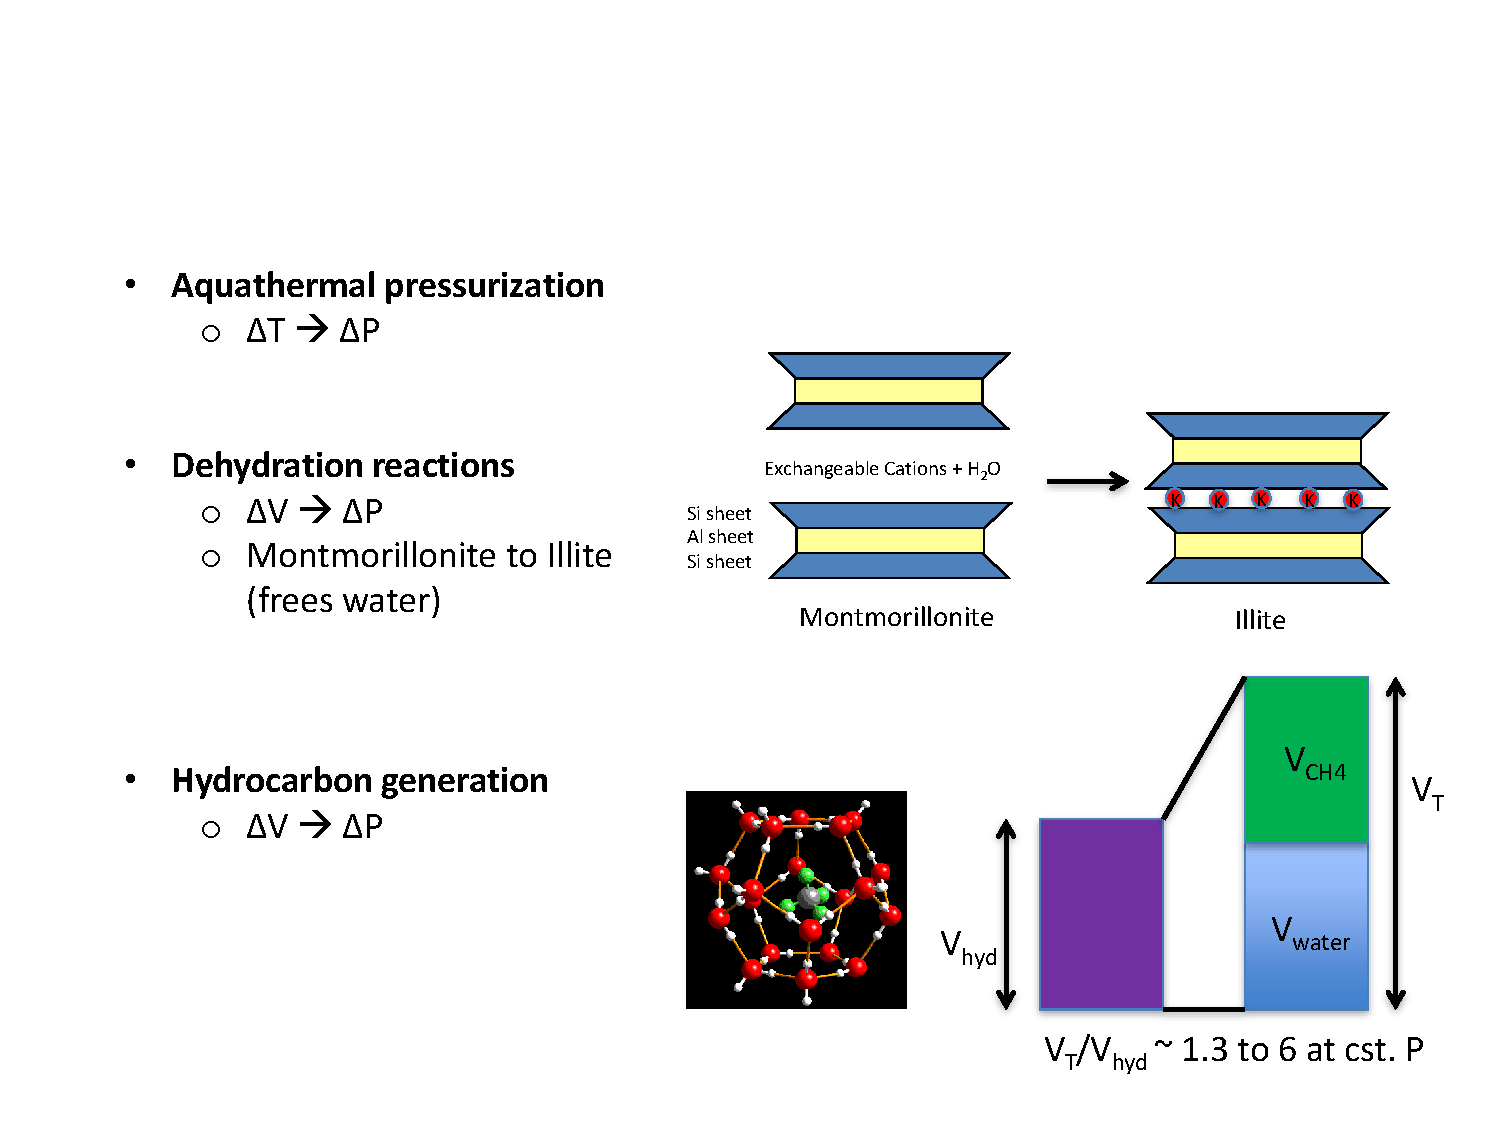
\includegraphics[scale=0.50]{.././Figures/split/2-11.pdf}%
\lthtmlpictureZ
\lthtmlcheckvsize\clearpage}

\stepcounter{subsection}
{\newpage\clearpage
\lthtmlinlinemathA{tex2html_wrap_inline15390}%
$ W$%
\lthtmlindisplaymathZ
\lthtmlcheckvsize\clearpage}

{\newpage\clearpage
\lthtmlinlinemathA{tex2html_wrap_inline15392}%
$ \Delta P = W/A$%
\lthtmlindisplaymathZ
\lthtmlcheckvsize\clearpage}

{\newpage\clearpage
\lthtmlinlinemathA{tex2html_wrap_inline15400}%
$ \sigma_v = W/A$%
\lthtmlindisplaymathZ
\lthtmlcheckvsize\clearpage}

{\newpage\clearpage
\lthtmlinlinemathA{tex2html_wrap_inline15404}%
$ \Delta P = 0$%
\lthtmlindisplaymathZ
\lthtmlcheckvsize\clearpage}

{\newpage\clearpage
\lthtmlpictureA{tex2html_wrap15408}%
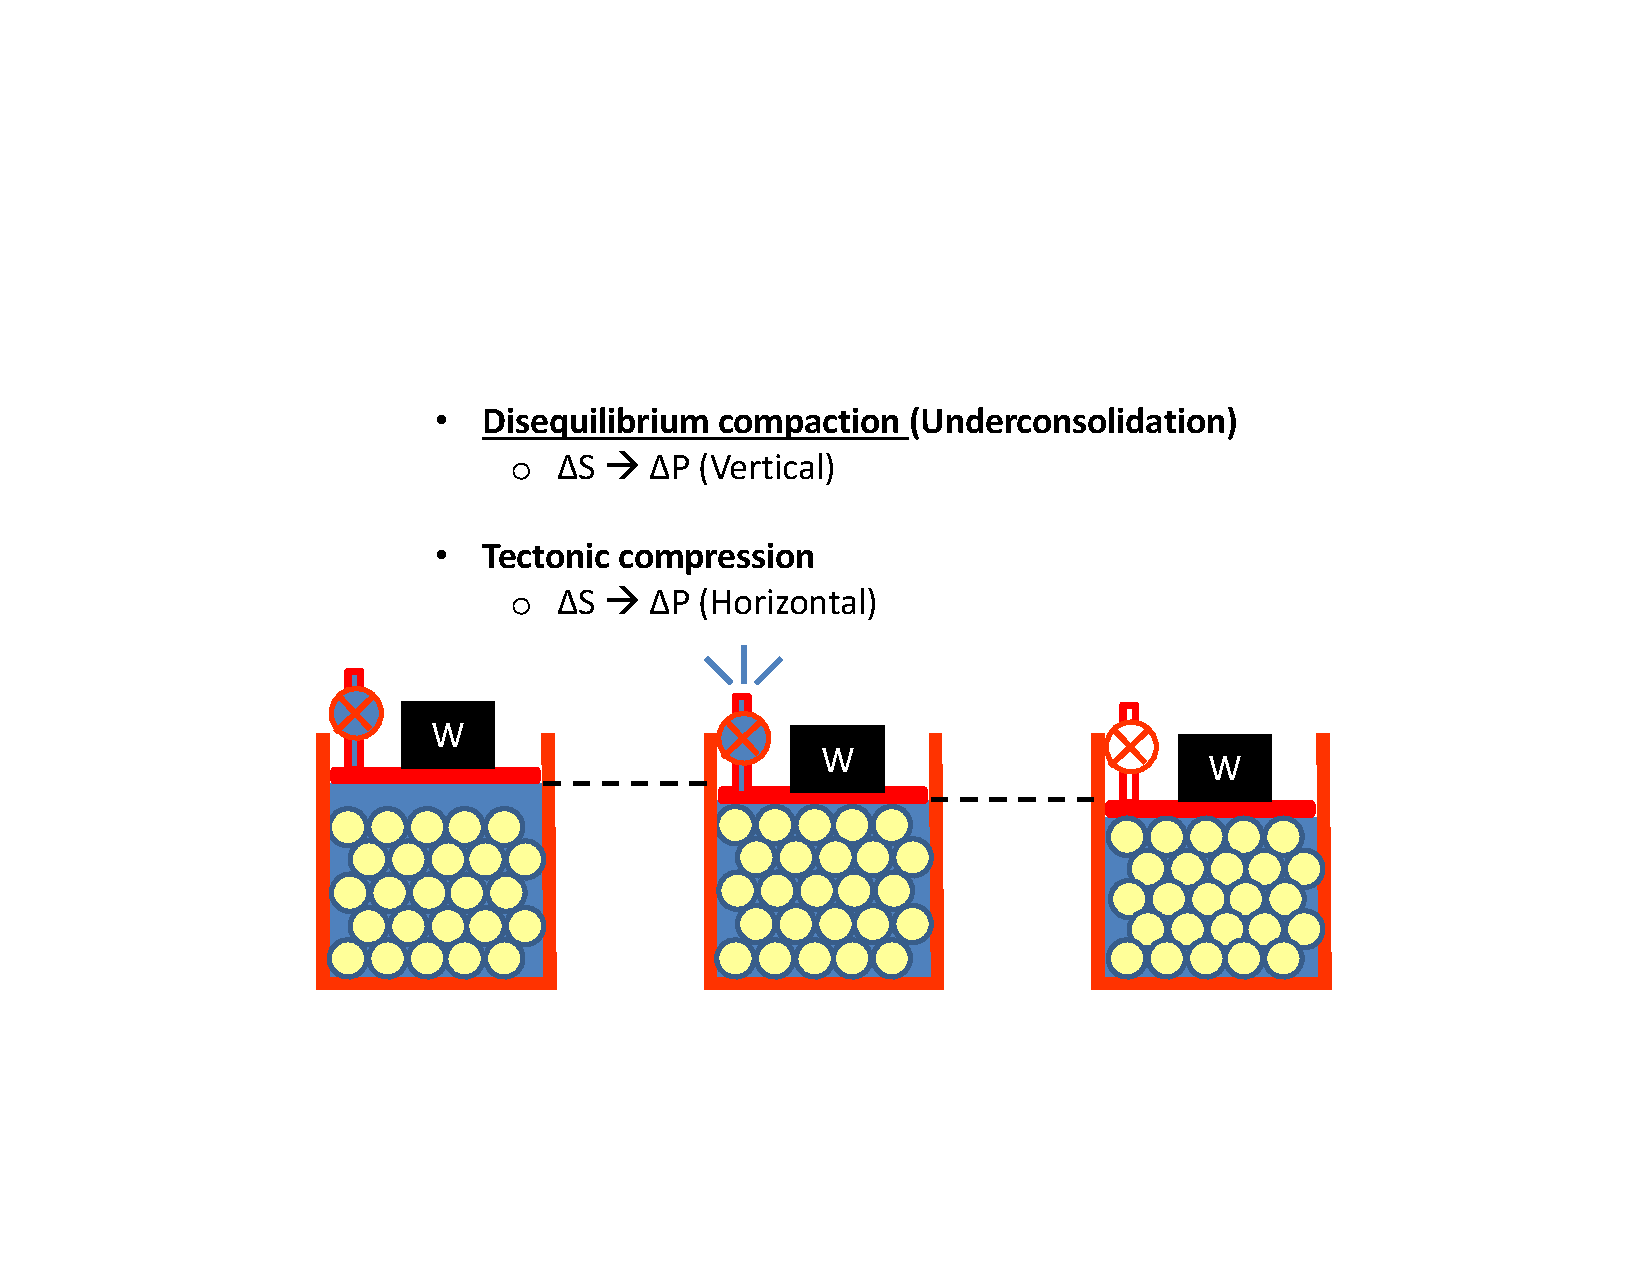
\includegraphics[scale=0.50]{.././Figures/split/2-12.pdf}%
\lthtmlpictureZ
\lthtmlcheckvsize\clearpage}

{\newpage\clearpage
\lthtmlpictureA{tex2html_wrap15413}%
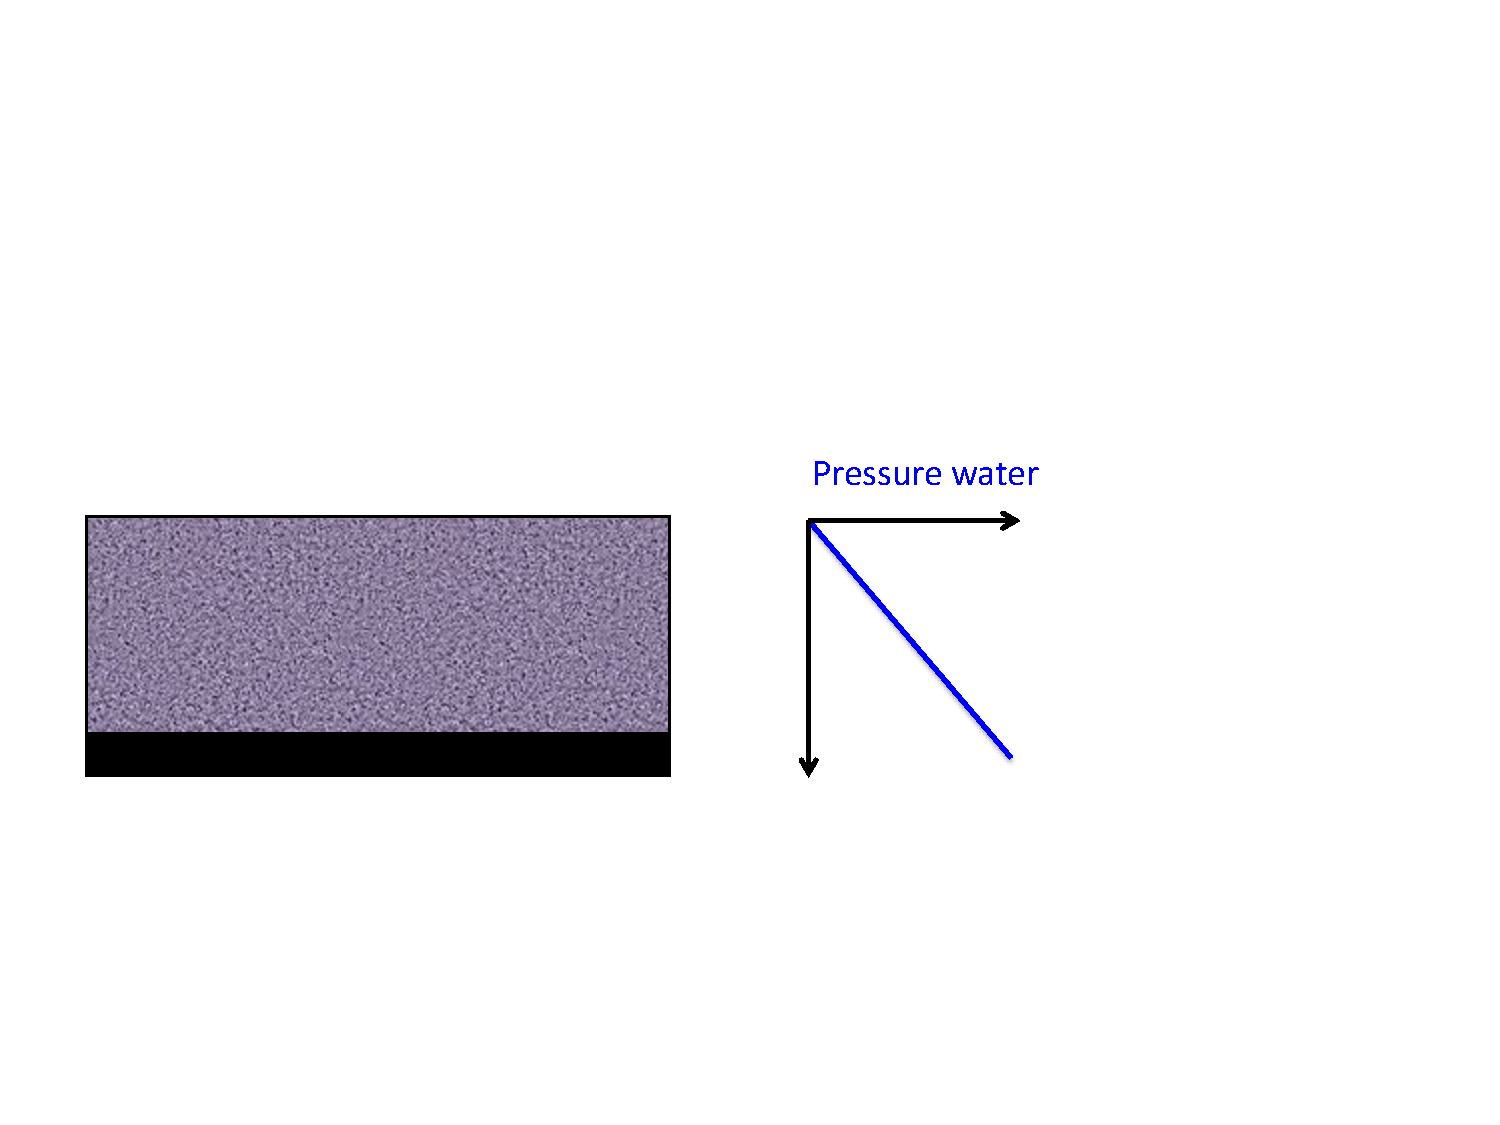
\includegraphics[scale=0.60]{.././Figures/split/2-13.pdf}%
\lthtmlpictureZ
\lthtmlcheckvsize\clearpage}

{\newpage\clearpage
\lthtmlinlinemathA{tex2html_wrap_inline15418}%
$ \Delta z$%
\lthtmlindisplaymathZ
\lthtmlcheckvsize\clearpage}

{\newpage\clearpage
\lthtmlinlinemathA{tex2html_wrap_indisplay15420}%
$\displaystyle D_h = \frac{M k} {\mu}$%
\lthtmlindisplaymathZ
\lthtmlcheckvsize\clearpage}

{\newpage\clearpage
\lthtmlinlinemathA{tex2html_wrap_inline15424}%
$ C_{bp}$%
\lthtmlindisplaymathZ
\lthtmlcheckvsize\clearpage}

{\newpage\clearpage
\lthtmlinlinemathA{tex2html_wrap_inline15426}%
$ k$%
\lthtmlindisplaymathZ
\lthtmlcheckvsize\clearpage}

{\newpage\clearpage
\lthtmlinlinemathA{tex2html_wrap_inline15428}%
$ \mu$%
\lthtmlindisplaymathZ
\lthtmlcheckvsize\clearpage}

{\newpage\clearpage
\lthtmlinlinemathA{tex2html_wrap_indisplay15430}%
$\displaystyle \frac{\partial P_p}{\partial t} = D_h \frac{d^2P_p}{dz^2}$%
\lthtmlindisplaymathZ
\lthtmlcheckvsize\clearpage}

{\newpage\clearpage
\lthtmlpictureA{tex2html_wrap15432}%
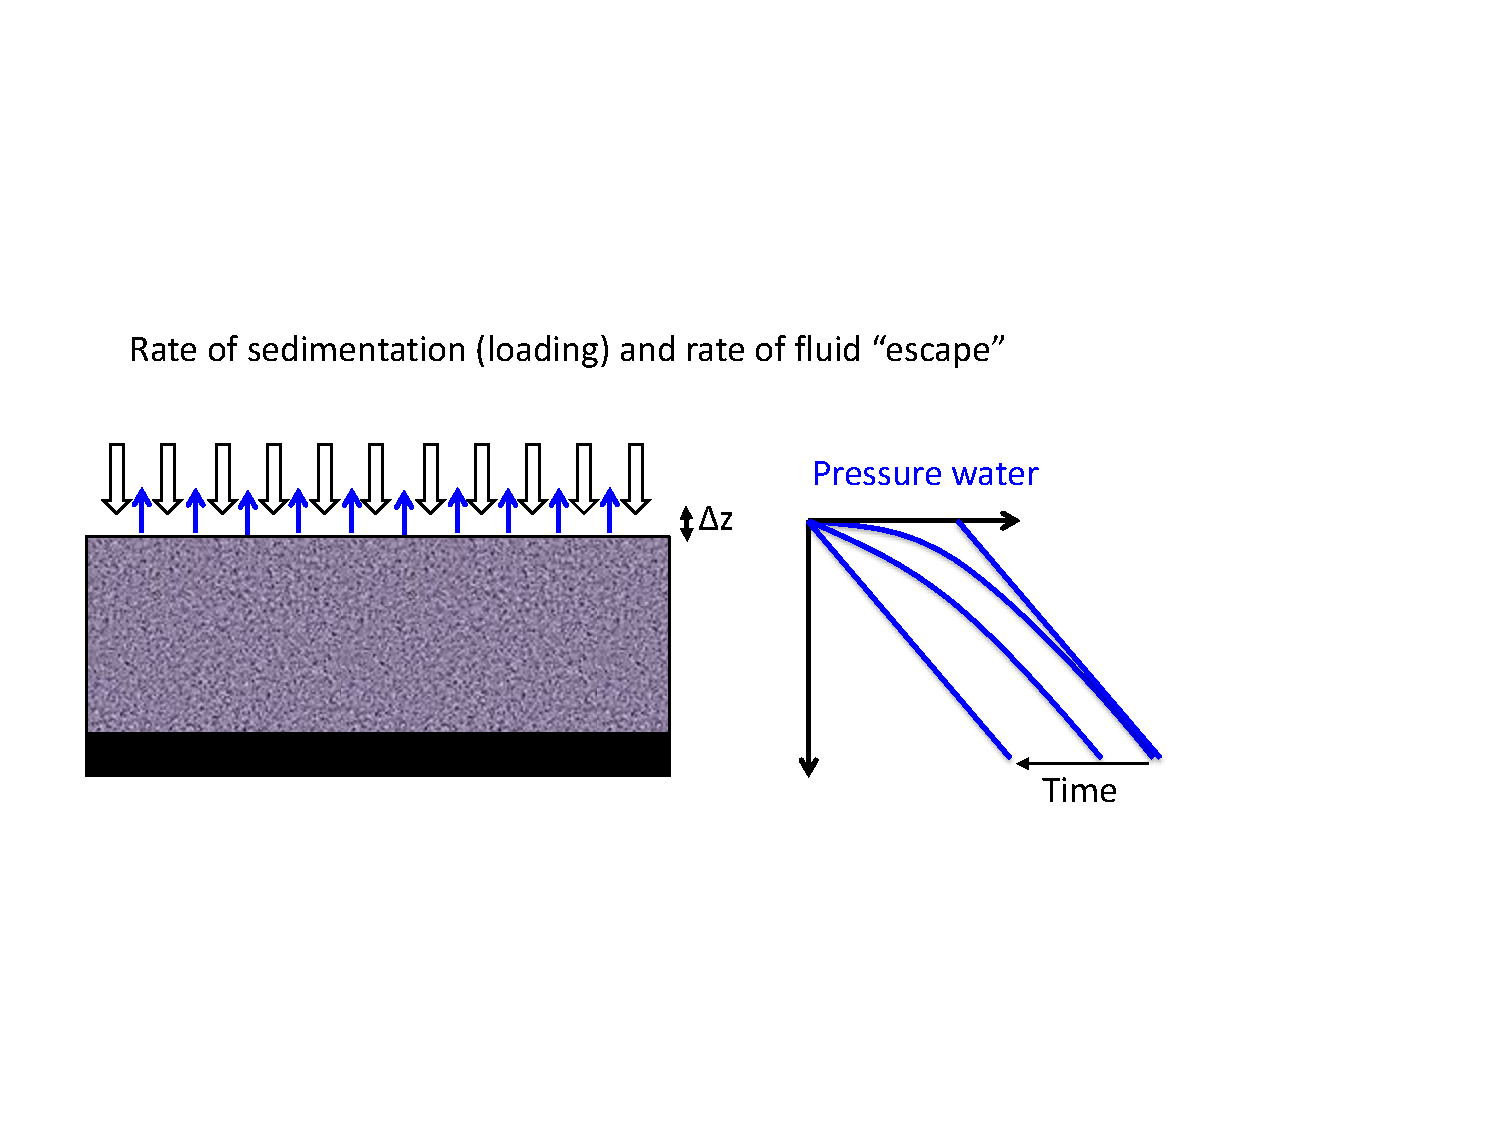
\includegraphics[scale=0.60]{.././Figures/split/2-14.pdf}%
\lthtmlpictureZ
\lthtmlcheckvsize\clearpage}

{\newpage\clearpage
\lthtmlinlinemathA{tex2html_wrap_inline15437}%
$ T_{ch}$%
\lthtmlindisplaymathZ
\lthtmlcheckvsize\clearpage}

{\newpage\clearpage
\lthtmlinlinemathA{tex2html_wrap_inline15439}%
$ \sim 2/3$%
\lthtmlindisplaymathZ
\lthtmlcheckvsize\clearpage}

{\newpage\clearpage
\lthtmlinlinemathA{tex2html_wrap_indisplay15441}%
$\displaystyle T_{ch} = \frac{L^2}{D_h}$%
\lthtmlindisplaymathZ
\lthtmlcheckvsize\clearpage}

{\newpage\clearpage
\lthtmlinlinemathA{tex2html_wrap_inline15443}%
$ L$%
\lthtmlindisplaymathZ
\lthtmlcheckvsize\clearpage}

{\newpage\clearpage
\lthtmlinlinemathA{tex2html_wrap_inline15447}%
$ k =$%
\lthtmlindisplaymathZ
\lthtmlcheckvsize\clearpage}

{\newpage\clearpage
\lthtmlinlinemathA{tex2html_wrap_inline15449}%
$ M =$%
\lthtmlindisplaymathZ
\lthtmlcheckvsize\clearpage}

{\newpage\clearpage
\lthtmlinlinemathA{tex2html_wrap_inline15455}%
$ T_{ch} \sim $%
\lthtmlindisplaymathZ
\lthtmlcheckvsize\clearpage}

{\newpage\clearpage
\lthtmlinlinemathA{tex2html_wrap_indisplay15463}%
$\displaystyle \phi = \phi_o \exp (-\beta \sigma_v)$%
\lthtmlindisplaymathZ
\lthtmlcheckvsize\clearpage}

{\newpage\clearpage
\lthtmlpictureA{tex2html_wrap15465}%
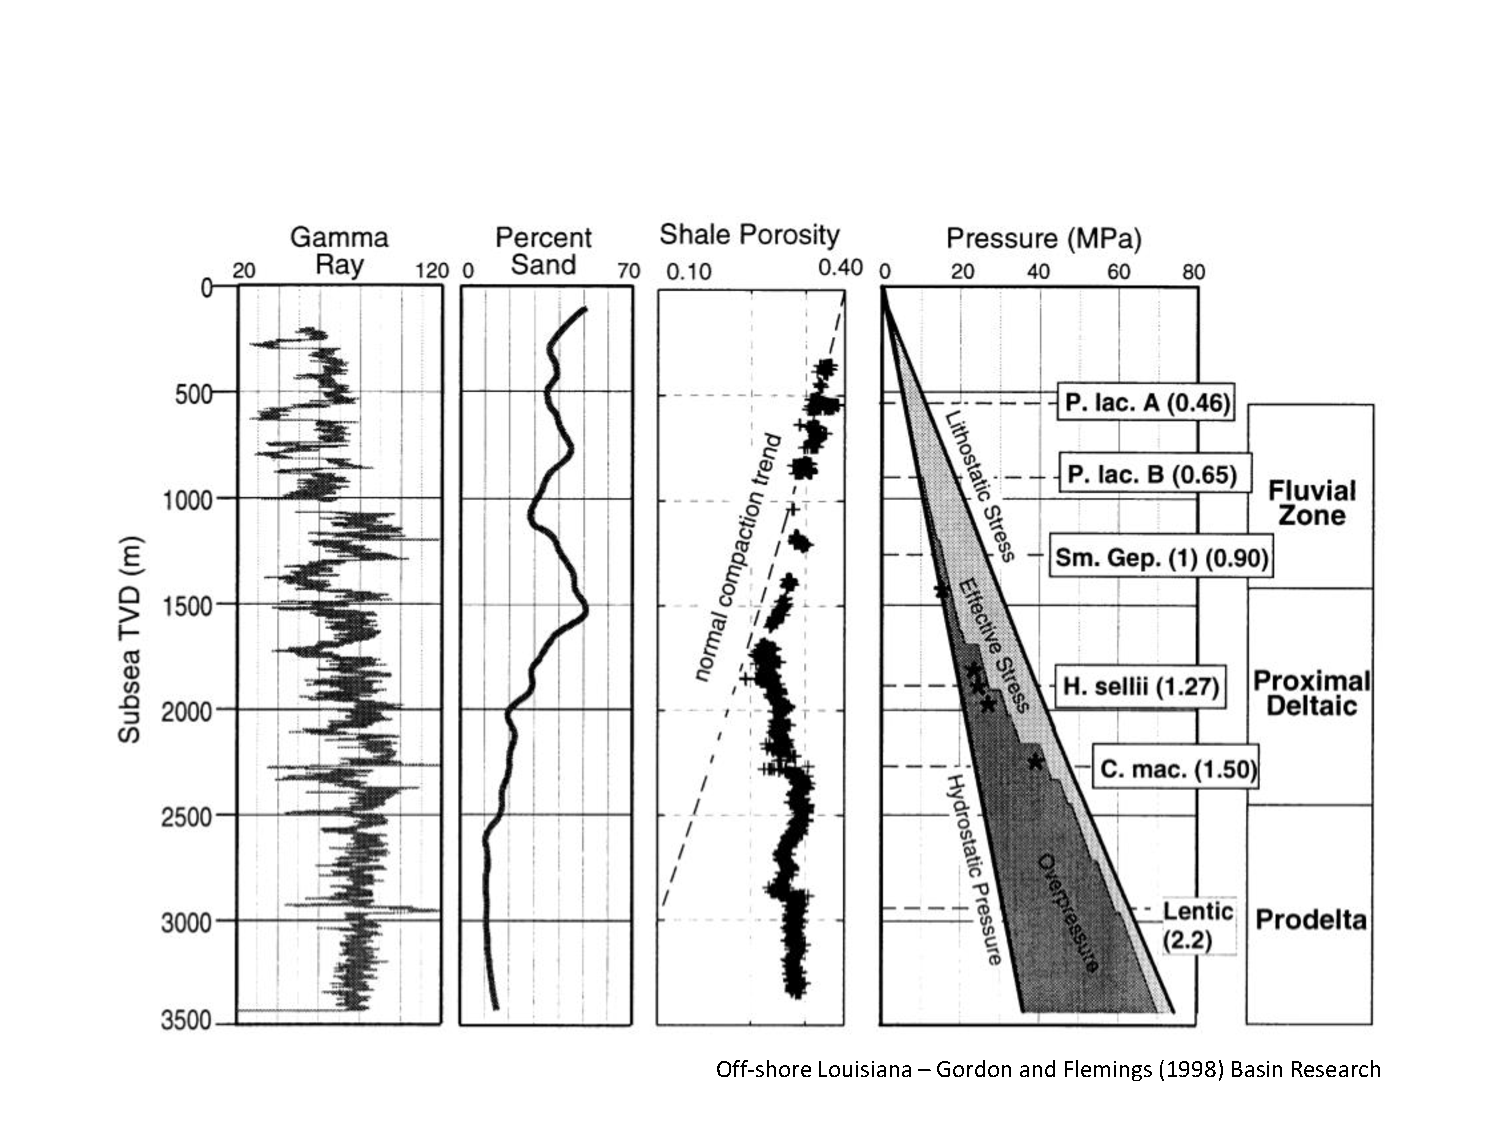
\includegraphics[scale=0.65]{.././Figures/split/2-16.pdf}%
\lthtmlpictureZ
\lthtmlcheckvsize\clearpage}

{\newpage\clearpage
\lthtmlinlinemathA{tex2html_wrap_inline15478}%
$ \phi = 0.298$%
\lthtmlindisplaymathZ
\lthtmlcheckvsize\clearpage}

{\newpage\clearpage
\lthtmlinlinemathA{tex2html_wrap_inline15480}%
$ \beta = 3.2 \times 10^{-2}$%
\lthtmlindisplaymathZ
\lthtmlcheckvsize\clearpage}

{\newpage\clearpage
\lthtmlinlinemathA{tex2html_wrap_inline15482}%
$ ^{-1}$%
\lthtmlindisplaymathZ
\lthtmlcheckvsize\clearpage}

{\newpage\clearpage
\lthtmlinlinemathA{tex2html_wrap_inline15484}%
$ \phi_0 = 0.38$%
\lthtmlindisplaymathZ
\lthtmlcheckvsize\clearpage}

{\newpage\clearpage
\lthtmlinlinemathA{tex2html_wrap_inline15486}%
$ S_v =$%
\lthtmlindisplaymathZ
\lthtmlcheckvsize\clearpage}

{\newpage\clearpage
\lthtmlinlinemathA{tex2html_wrap_inline15488}%
$ \times$%
\lthtmlindisplaymathZ
\lthtmlcheckvsize\clearpage}

{\newpage\clearpage
\lthtmlinlinemathA{tex2html_wrap_indisplay15492}%
$\displaystyle P_p = S_v + \frac{\ln \left( \phi / \phi_o \right)}{\beta} =
38$%
\lthtmlindisplaymathZ
\lthtmlcheckvsize\clearpage}

{\newpage\clearpage
\lthtmlinlinemathA{tex2html_wrap_indisplay15493}%
$\displaystyle - 7.6$%
\lthtmlindisplaymathZ
\lthtmlcheckvsize\clearpage}

{\newpage\clearpage
\lthtmlinlinemathA{tex2html_wrap_indisplay15494}%
$\displaystyle = 30.40$%
\lthtmlindisplaymathZ
\lthtmlcheckvsize\clearpage}

{\newpage\clearpage
\lthtmlinlinemathA{tex2html_wrap_indisplay15497}%
$\displaystyle \lambda_p = \frac{P_p}{S_v} = 	\frac{30.40 \text{ MPa}}{38 \text{ MPa}} = 0.8. \: \: \blacksquare$%
\lthtmlindisplaymathZ
\lthtmlcheckvsize\clearpage}

\stepcounter{subsection}
{\newpage\clearpage
\lthtmlpictureA{tex2html_wrap15500}%
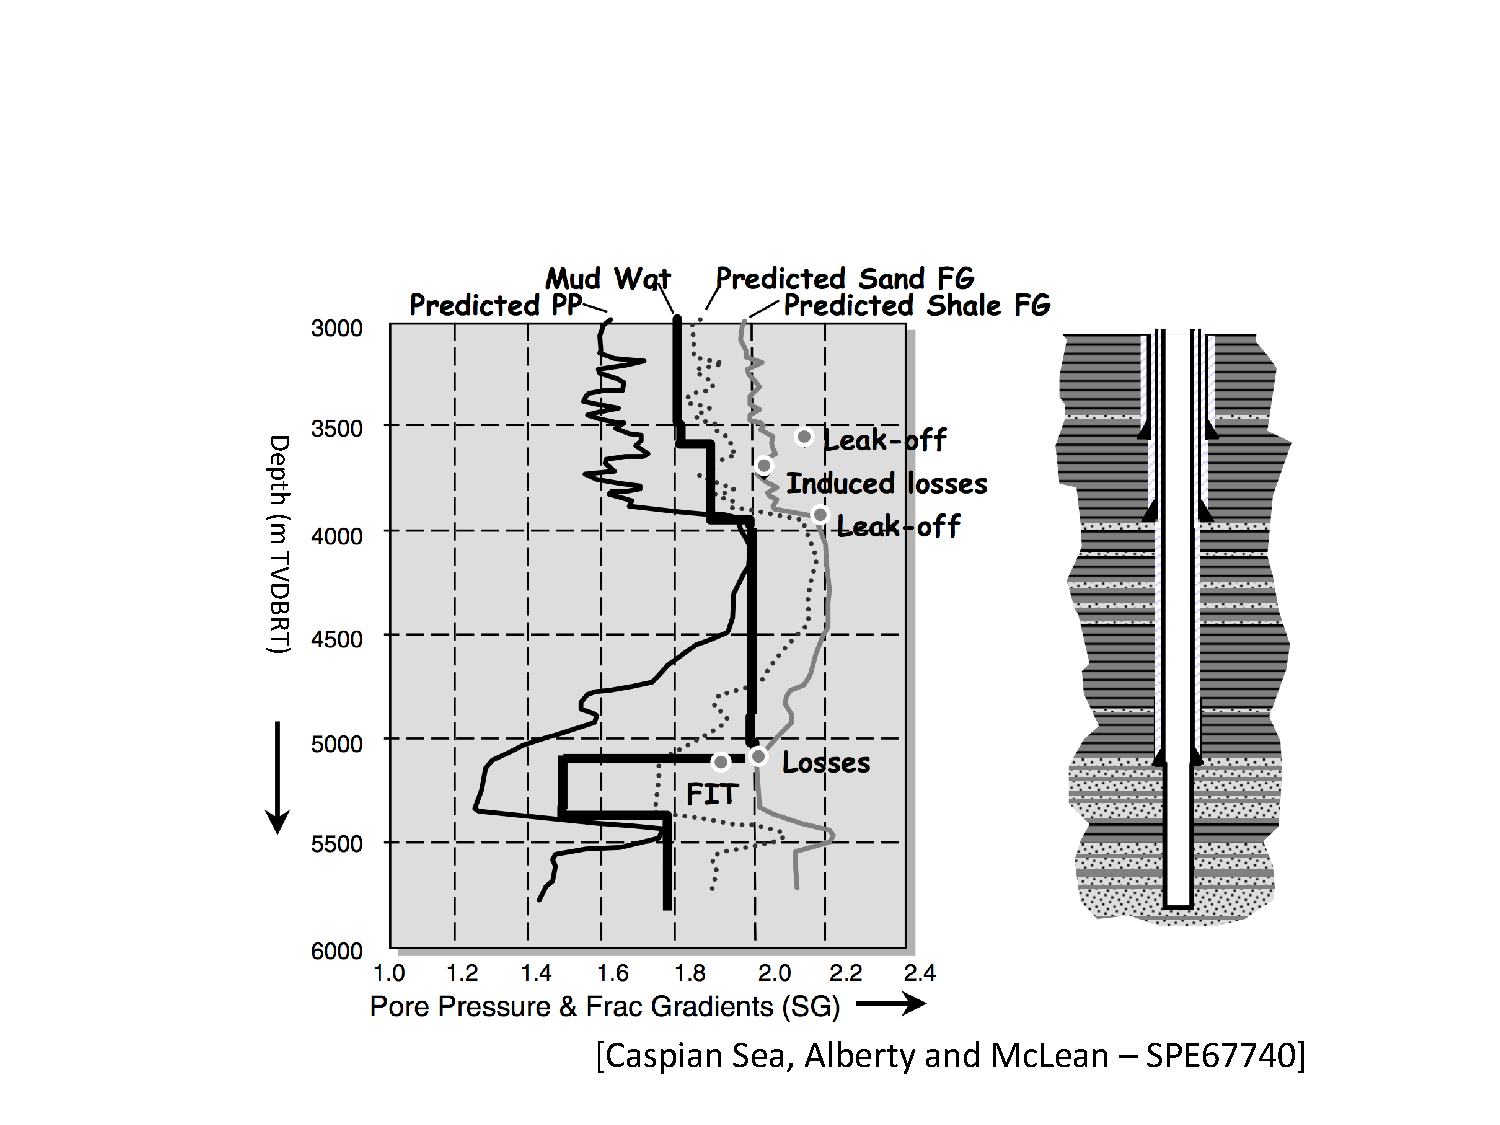
\includegraphics[scale=0.65]{.././Figures/split/2-17.pdf}%
\lthtmlpictureZ
\lthtmlcheckvsize\clearpage}

\stepcounter{section}
\stepcounter{subsection}
{\newpage\clearpage
\lthtmlinlinemathA{tex2html_wrap_inline15509}%
$ S_{Hmax}$%
\lthtmlindisplaymathZ
\lthtmlcheckvsize\clearpage}

{\newpage\clearpage
\lthtmlinlinemathA{tex2html_wrap_inline15511}%
$ S_{hmin}$%
\lthtmlindisplaymathZ
\lthtmlcheckvsize\clearpage}

{\newpage\clearpage
\lthtmlinlinemathA{tex2html_wrap_inline15513}%
$ S_{Hmax} \geq S_{hmin}$%
\lthtmlindisplaymathZ
\lthtmlcheckvsize\clearpage}

{\newpage\clearpage
\lthtmlpictureA{tex2html_wrap15515}%
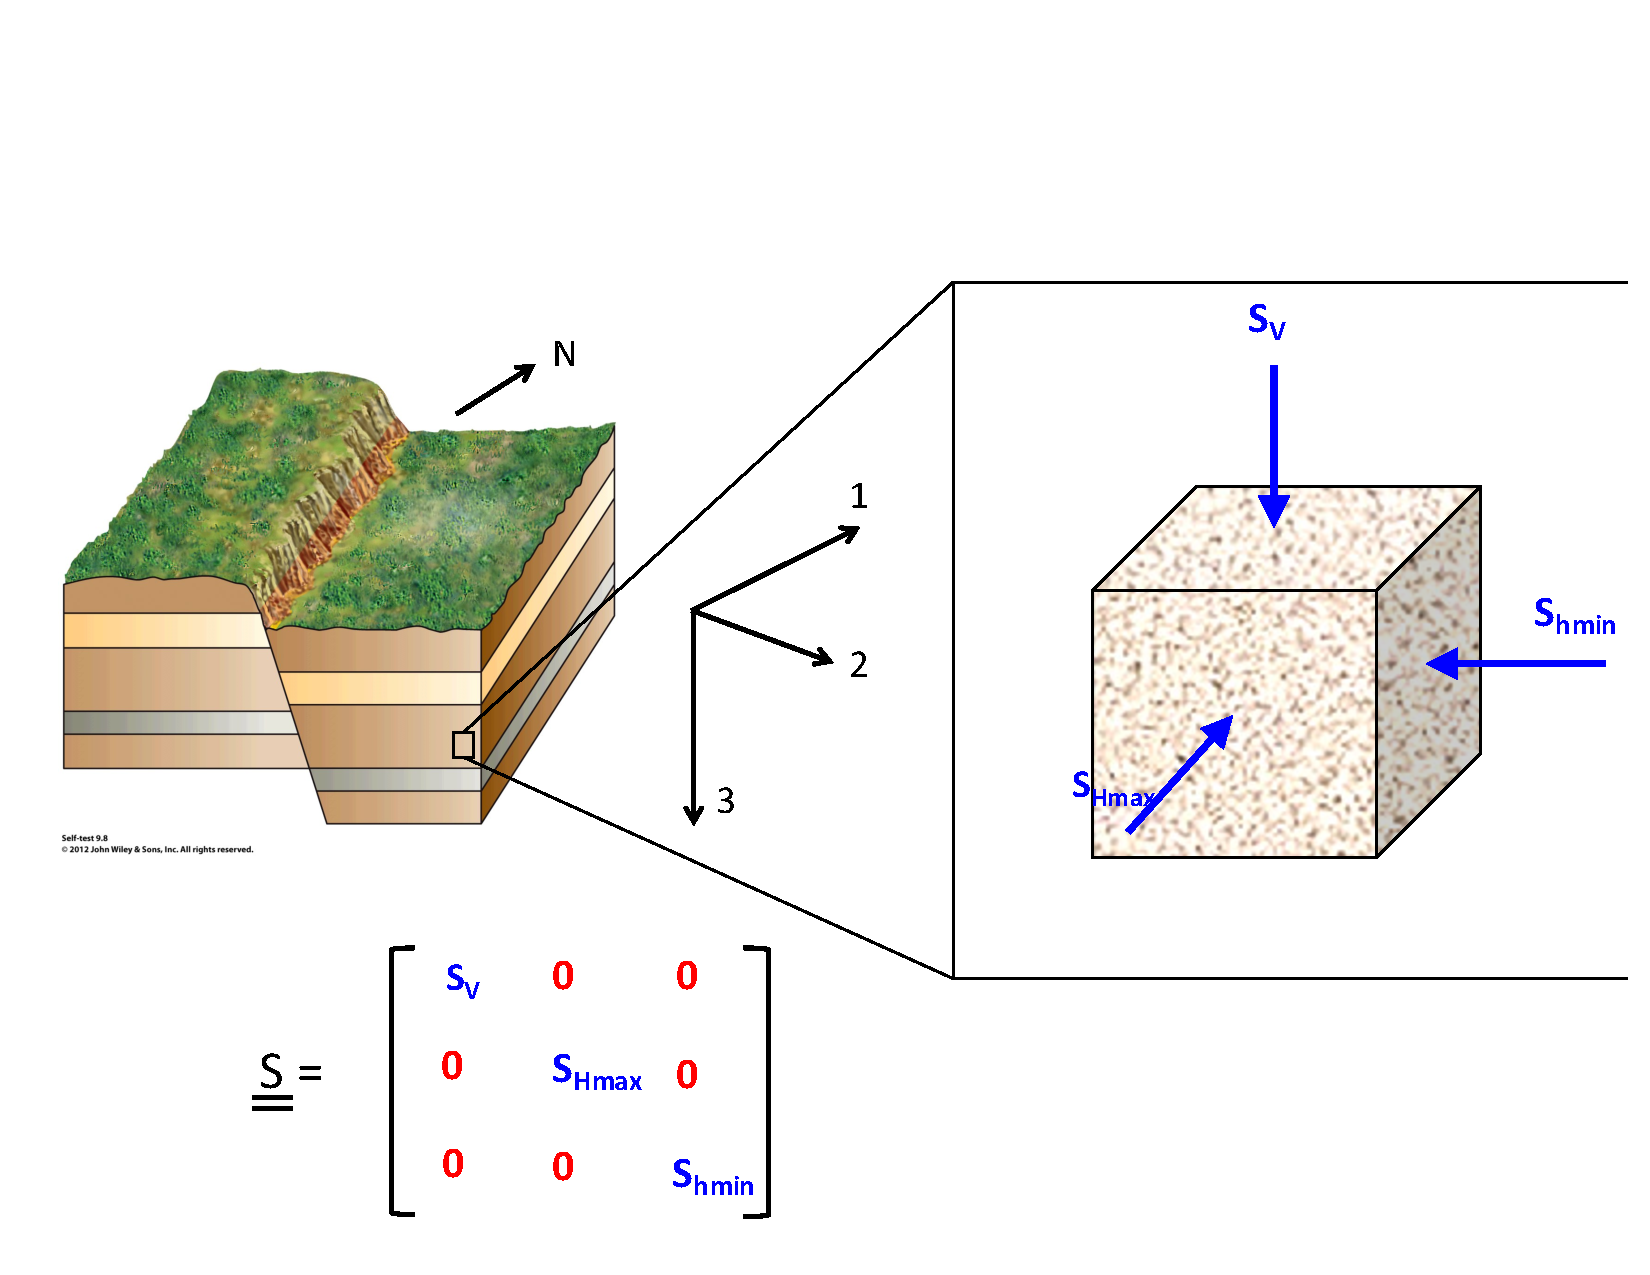
\includegraphics[scale=0.50]{.././Figures/split/3-20.pdf}%
\lthtmlpictureZ
\lthtmlcheckvsize\clearpage}

{\newpage\clearpage
\lthtmlpictureA{tex2html_wrap15520}%
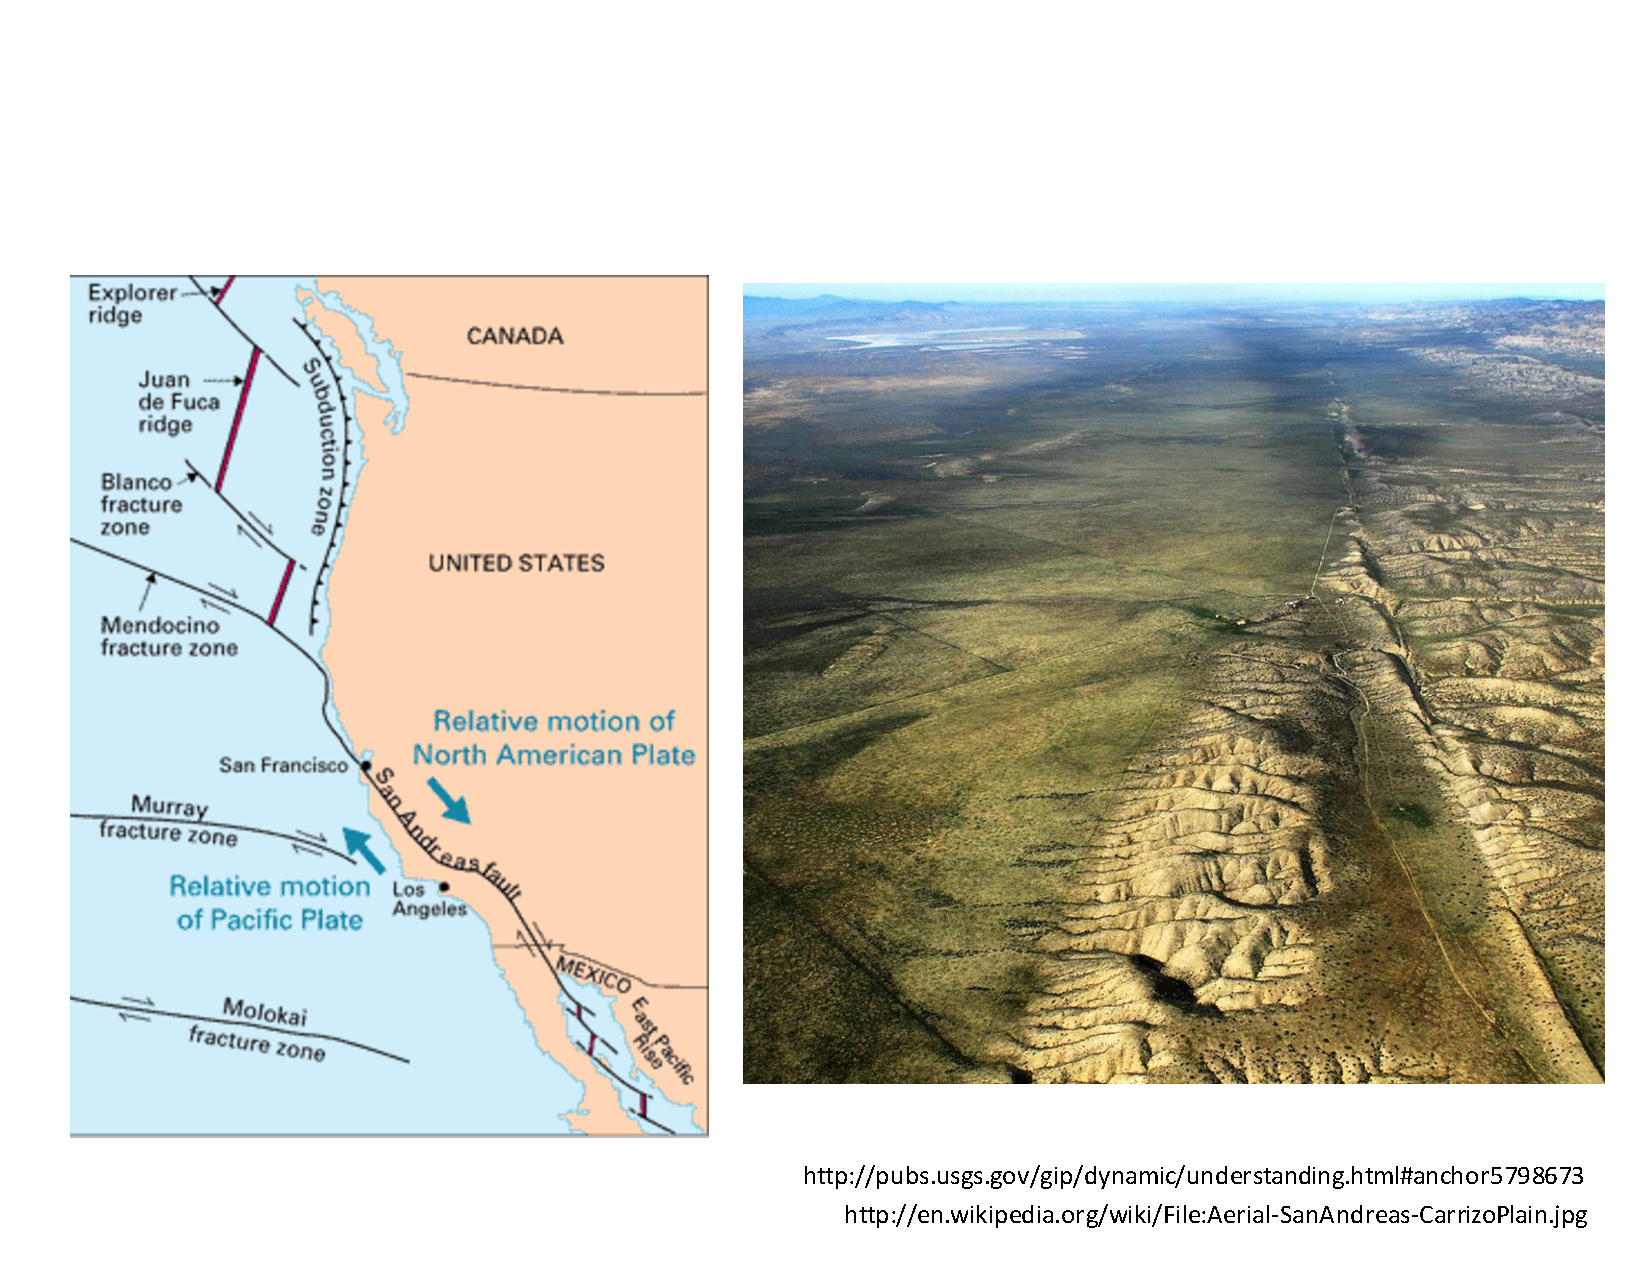
\includegraphics[scale=0.50]{.././Figures/split/3-16.pdf}%
\lthtmlpictureZ
\lthtmlcheckvsize\clearpage}

{\newpage\clearpage
\lthtmlpictureA{tex2html_wrap15525}%
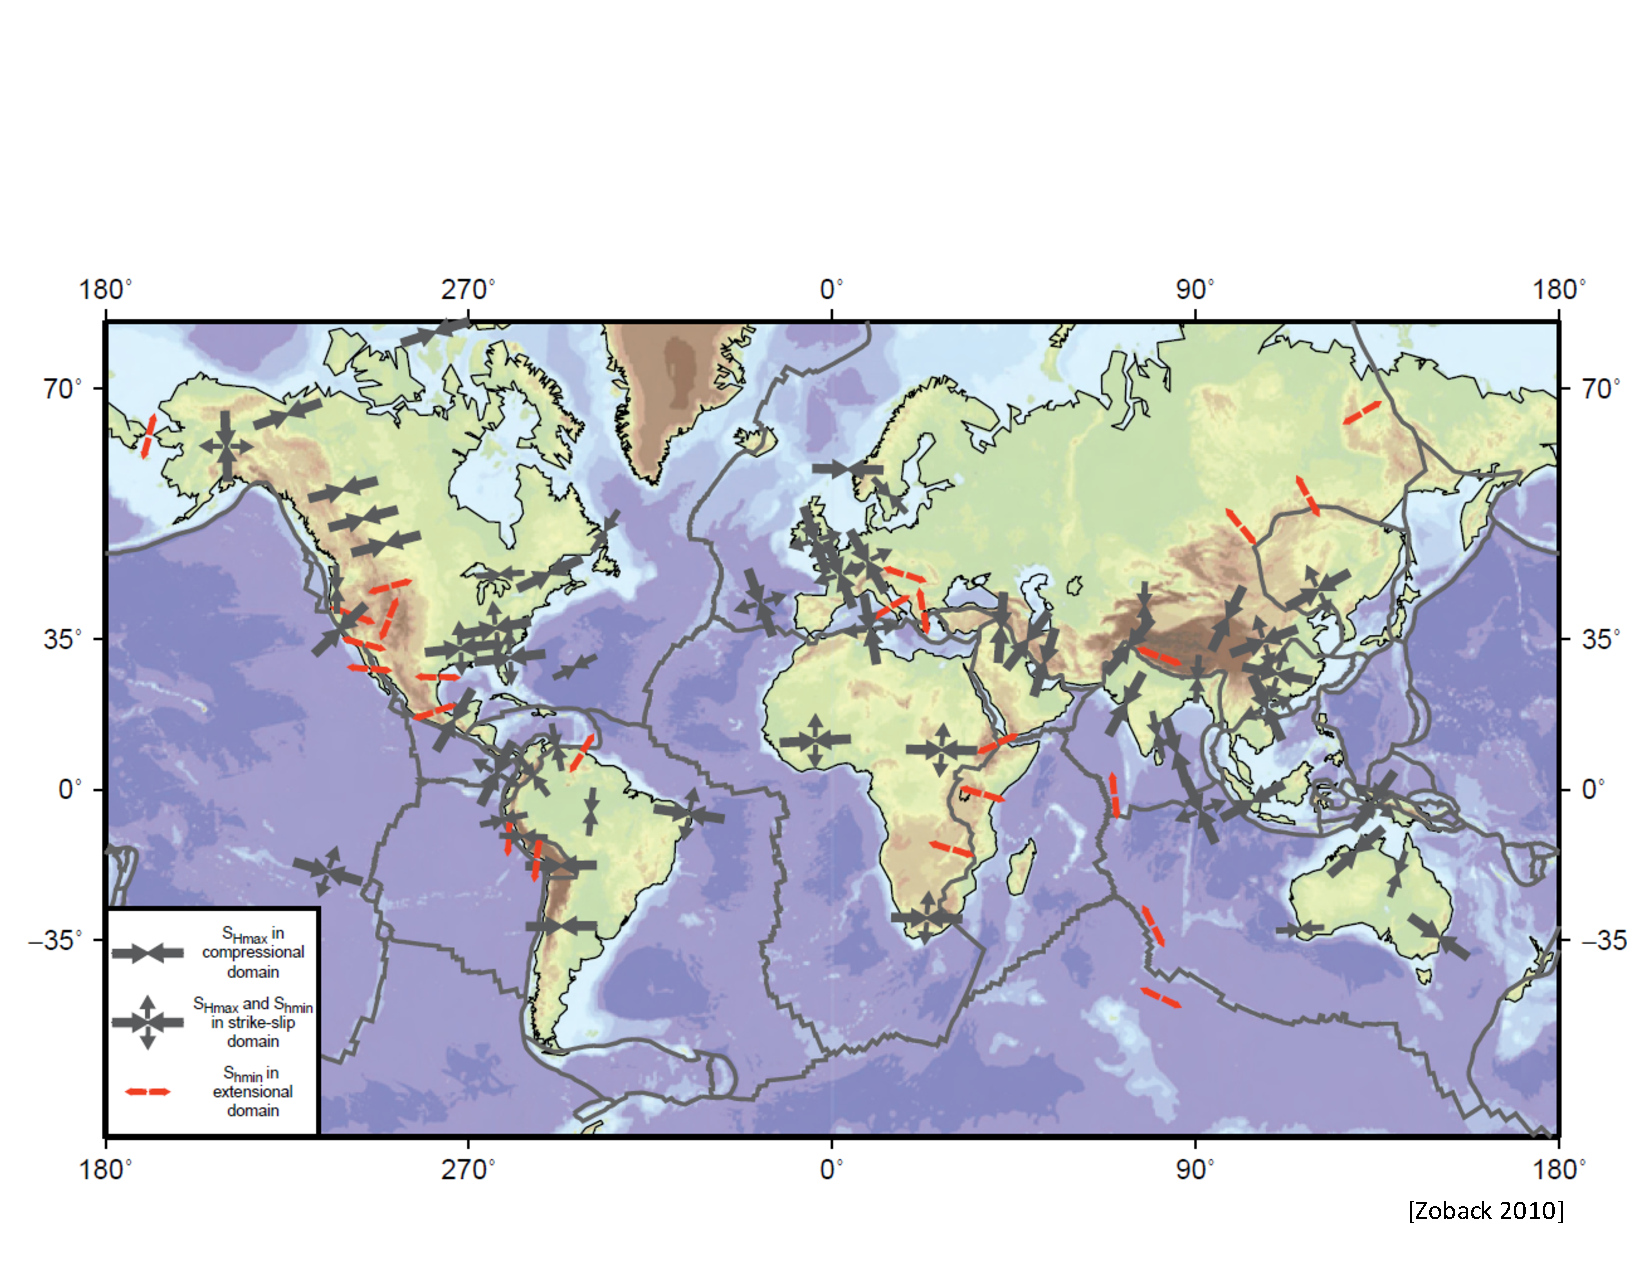
\includegraphics[scale=0.55]{.././Figures/split/3-18.pdf}%
\lthtmlpictureZ
\lthtmlcheckvsize\clearpage}

\stepcounter{subsection}
{\newpage\clearpage
\lthtmlpictureA{tex2html_wrap15533}%
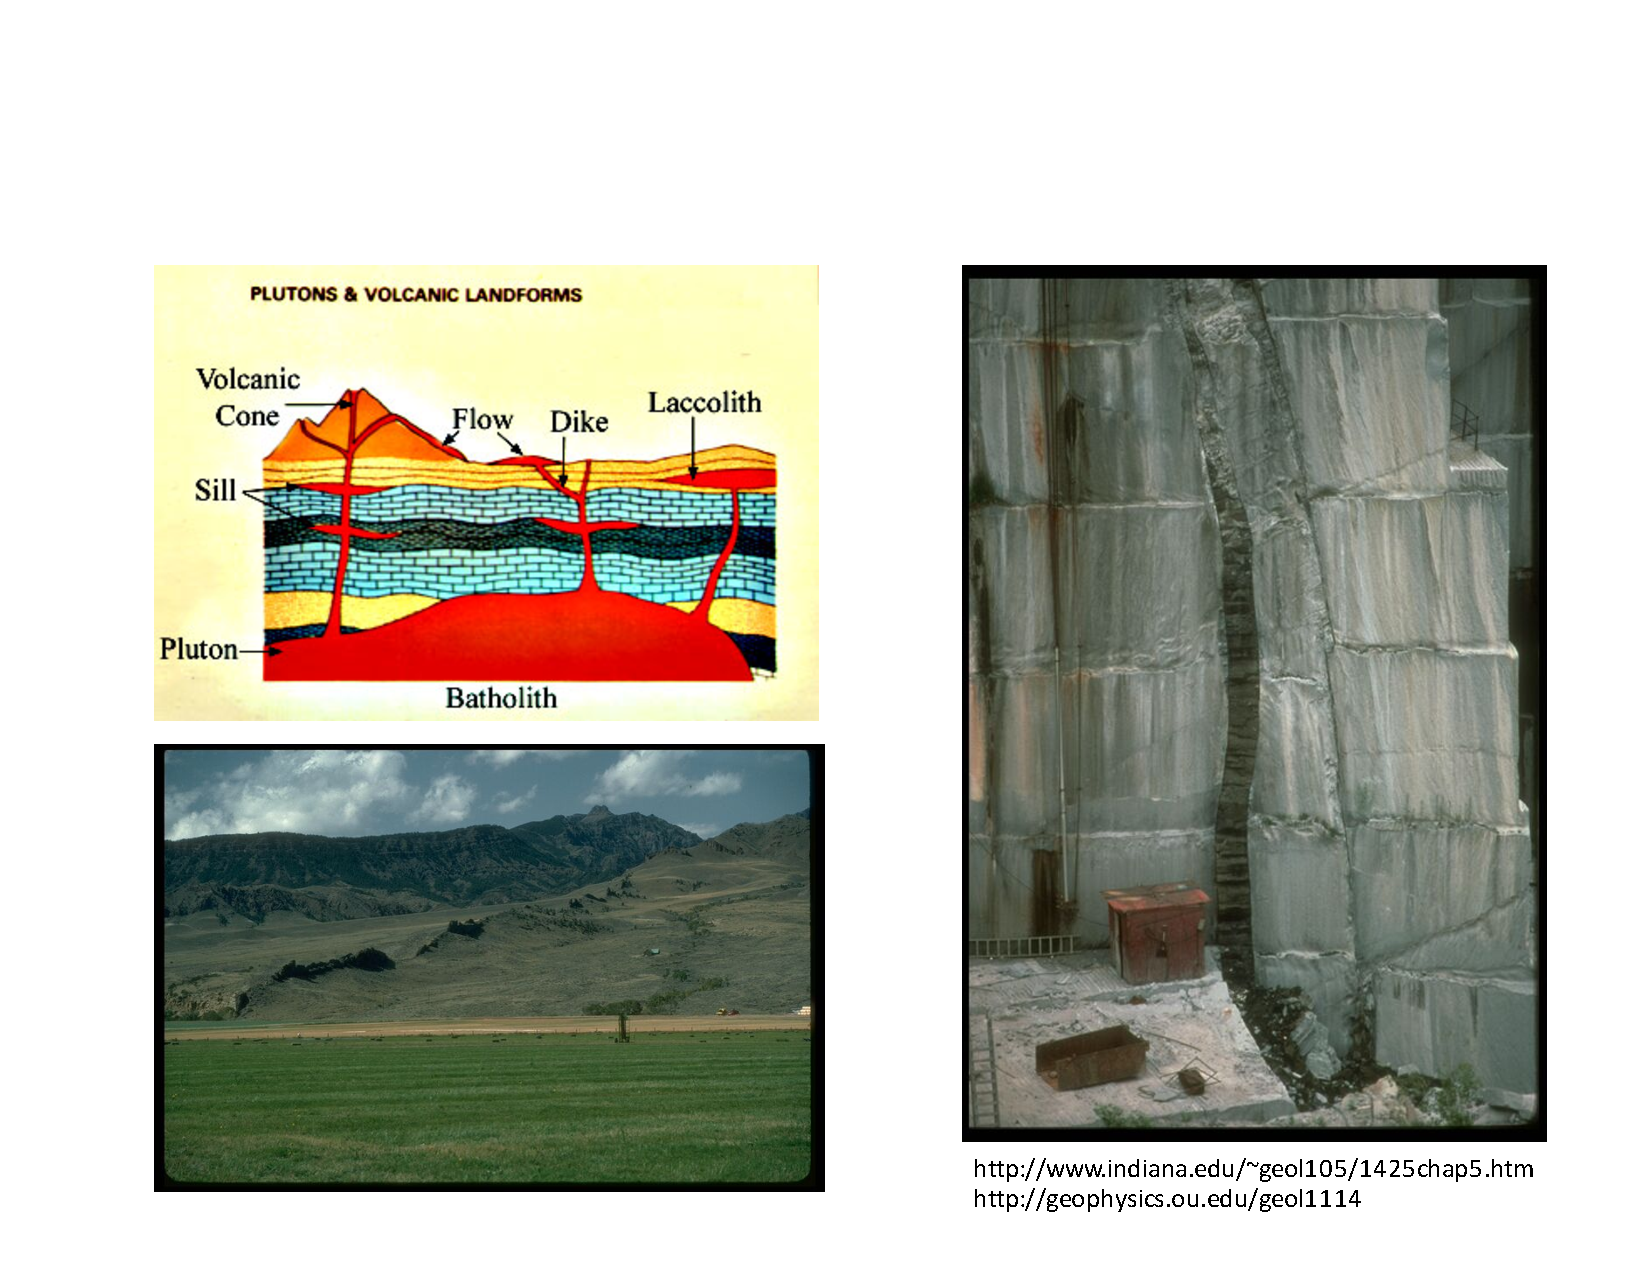
\includegraphics[scale=0.55]{.././Figures/split/3-2.pdf}%
\lthtmlpictureZ
\lthtmlcheckvsize\clearpage}

\stepcounter{subsection}
{\newpage\clearpage
\lthtmlinlinemathA{tex2html_wrap_inline15541}%
$ S_v > S_{hmin} = S_3$%
\lthtmlindisplaymathZ
\lthtmlcheckvsize\clearpage}

\stepcounter{subsection}
{\newpage\clearpage
\lthtmlinlinemathA{tex2html_wrap_inline15566}%
$ S_1$%
\lthtmlindisplaymathZ
\lthtmlcheckvsize\clearpage}

{\newpage\clearpage
\lthtmlinlinemathA{tex2html_wrap_inline15568}%
$ S_2$%
\lthtmlindisplaymathZ
\lthtmlcheckvsize\clearpage}

\stepcounter{subsubsection}
{\newpage\clearpage
\lthtmlinlinemathA{tex2html_wrap_inline15583}%
$ S_v > S_{Hmax} > S_{hmin}$%
\lthtmlindisplaymathZ
\lthtmlcheckvsize\clearpage}

{\newpage\clearpage
\lthtmlinlinemathA{tex2html_wrap_inline15585}%
$ S_1 = S_v$%
\lthtmlindisplaymathZ
\lthtmlcheckvsize\clearpage}

{\newpage\clearpage
\lthtmlinlinemathA{tex2html_wrap_inline15587}%
$ S_2 = S_{Hmax}$%
\lthtmlindisplaymathZ
\lthtmlcheckvsize\clearpage}

{\newpage\clearpage
\lthtmlinlinemathA{tex2html_wrap_inline15589}%
$ S_3 = S_{hmin}$%
\lthtmlindisplaymathZ
\lthtmlcheckvsize\clearpage}

{\newpage\clearpage
\lthtmlinlinemathA{tex2html_wrap_inline15593}%
$ \sim 60$%
\lthtmlindisplaymathZ
\lthtmlcheckvsize\clearpage}

{\newpage\clearpage
\lthtmlinlinemathA{tex2html_wrap_inline15597}%
$ \sigma_1 = S_1 - P_p$%
\lthtmlindisplaymathZ
\lthtmlcheckvsize\clearpage}

{\newpage\clearpage
\lthtmlinlinemathA{tex2html_wrap_inline15599}%
$ \sigma_3 = S_3 - P_p$%
\lthtmlindisplaymathZ
\lthtmlcheckvsize\clearpage}

{\newpage\clearpage
\lthtmlpictureA{tex2html_wrap15603}%
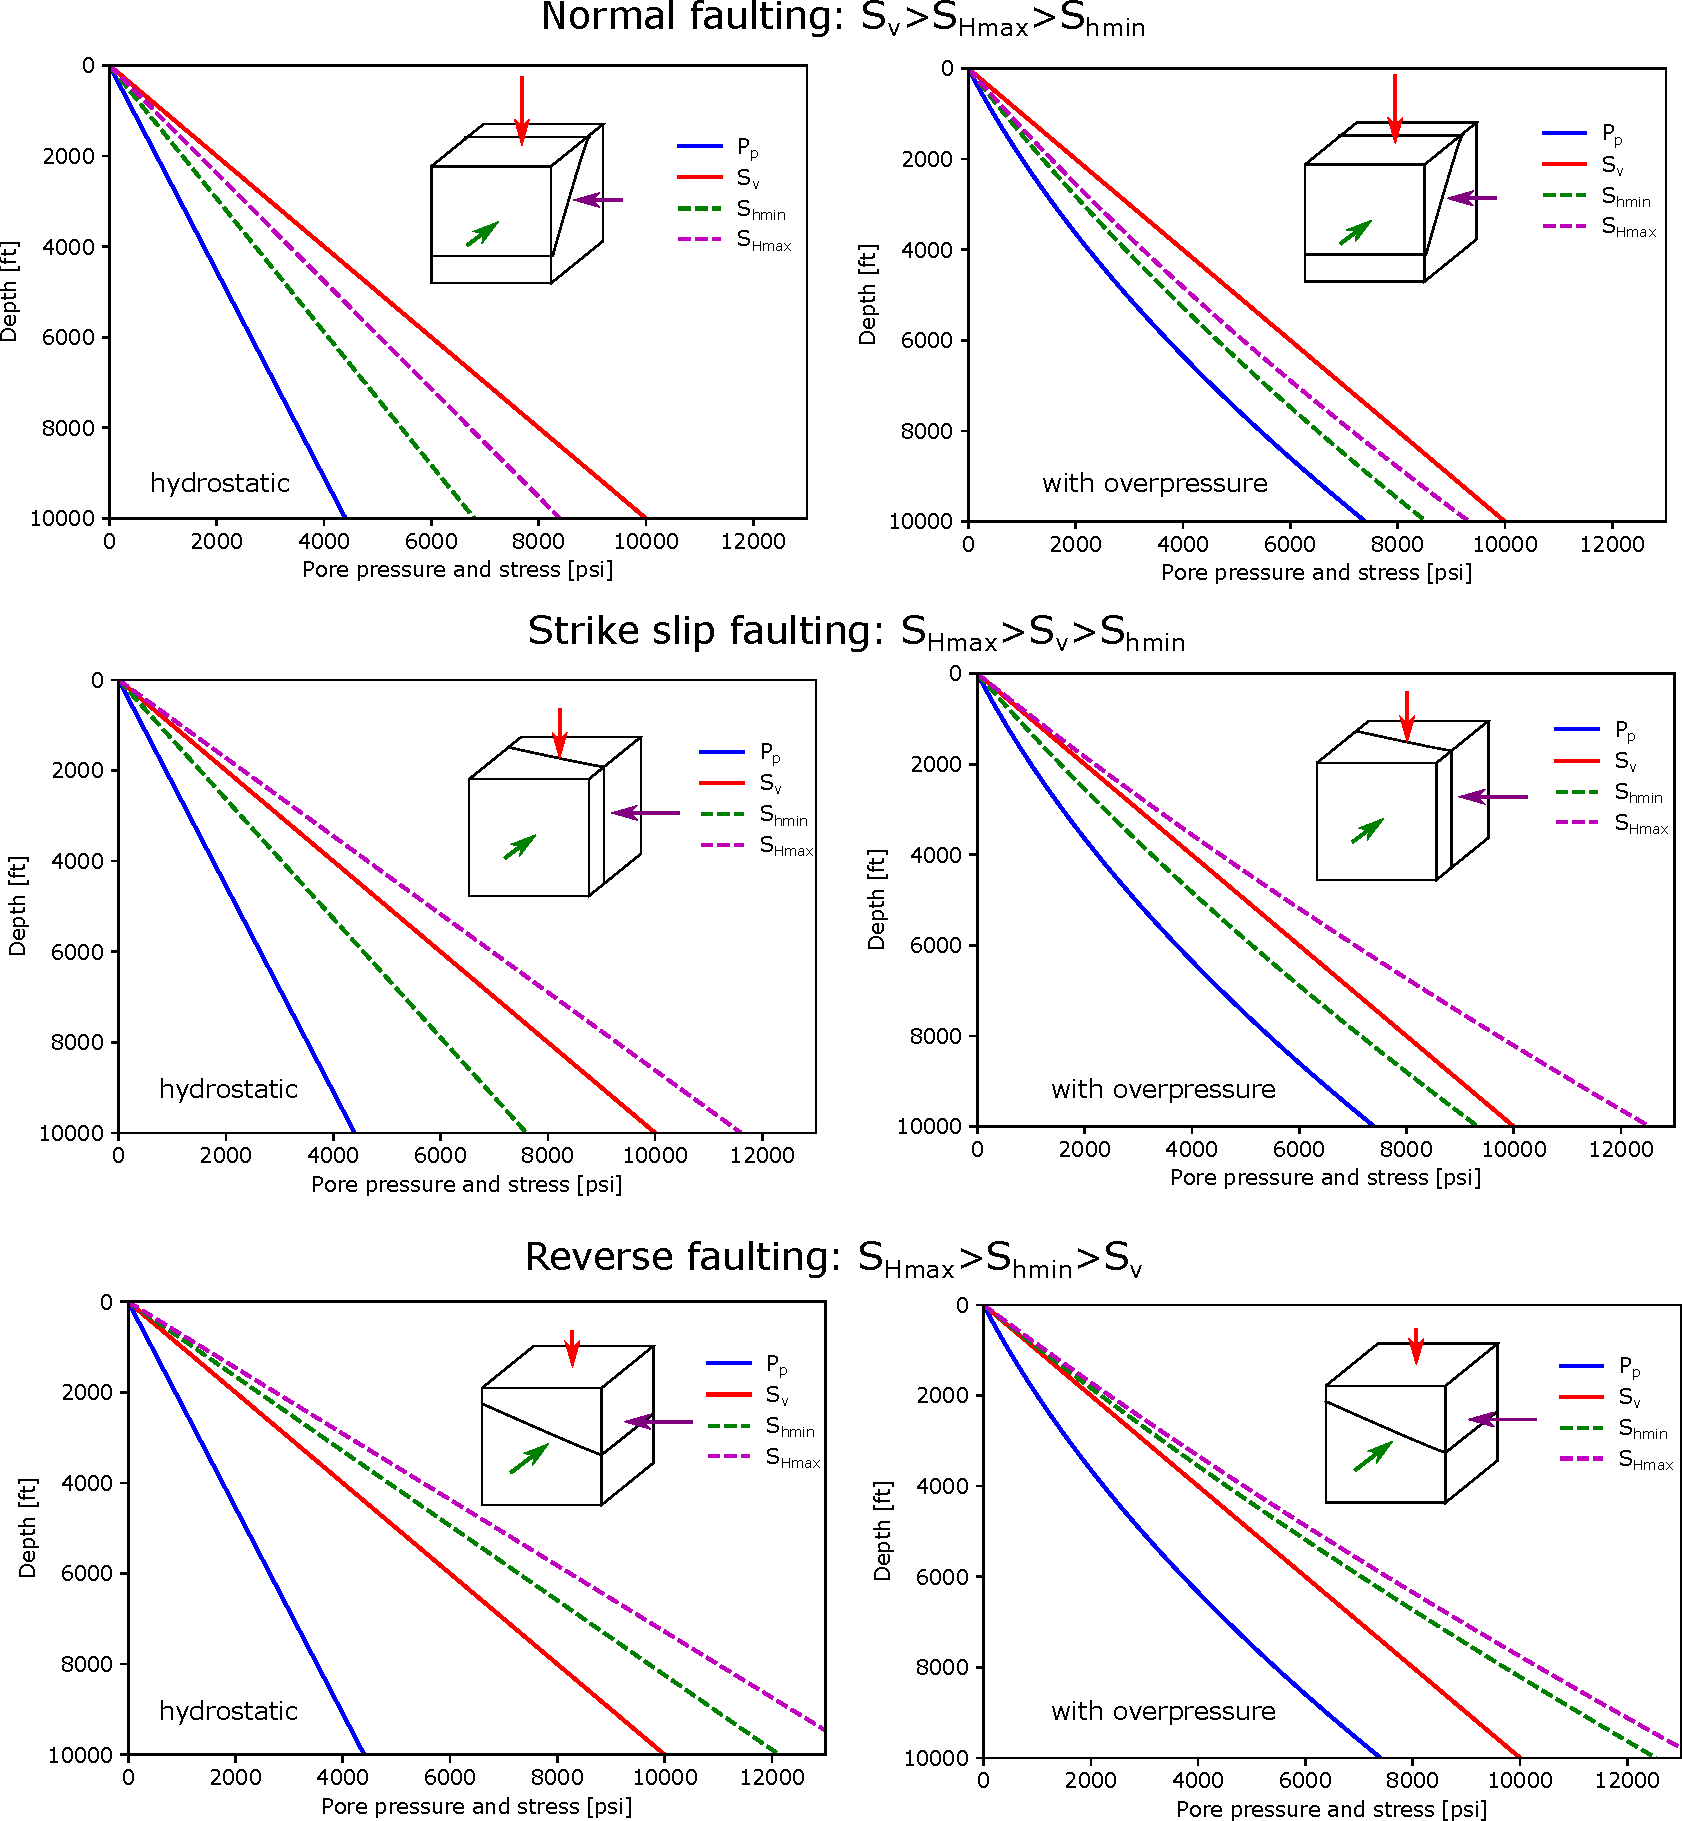
\includegraphics[scale=0.55]{.././Figures/split/2-StressProfiles.pdf}%
\lthtmlpictureZ
\lthtmlcheckvsize\clearpage}

\stepcounter{subsubsection}
{\newpage\clearpage
\lthtmlinlinemathA{tex2html_wrap_inline15609}%
$ S_{Hmax} > S_v > S_{hmin}$%
\lthtmlindisplaymathZ
\lthtmlcheckvsize\clearpage}

{\newpage\clearpage
\lthtmlinlinemathA{tex2html_wrap_inline15611}%
$ S_1 = S_{Hmax}$%
\lthtmlindisplaymathZ
\lthtmlcheckvsize\clearpage}

{\newpage\clearpage
\lthtmlinlinemathA{tex2html_wrap_inline15613}%
$ S_2 = S_v$%
\lthtmlindisplaymathZ
\lthtmlcheckvsize\clearpage}

\stepcounter{subsubsection}
{\newpage\clearpage
\lthtmlinlinemathA{tex2html_wrap_inline15624}%
$ S_{Hmax} > S_{hmin} > S_v$%
\lthtmlindisplaymathZ
\lthtmlcheckvsize\clearpage}

{\newpage\clearpage
\lthtmlinlinemathA{tex2html_wrap_inline15628}%
$ S_2 = S_{hmin}$%
\lthtmlindisplaymathZ
\lthtmlcheckvsize\clearpage}

{\newpage\clearpage
\lthtmlinlinemathA{tex2html_wrap_inline15630}%
$ S_3 = S_v$%
\lthtmlindisplaymathZ
\lthtmlcheckvsize\clearpage}

\stepcounter{subsection}
{\newpage\clearpage
\lthtmlinlinemathA{tex2html_wrap_inline15639}%
$ \rho_w g z$%
\lthtmlindisplaymathZ
\lthtmlcheckvsize\clearpage}

{\newpage\clearpage
\lthtmlinlinemathA{tex2html_wrap_inline15655}%
$ S_3 = S_{22}$%
\lthtmlindisplaymathZ
\lthtmlcheckvsize\clearpage}

{\newpage\clearpage
\lthtmlinlinemathA{tex2html_wrap_inline15657}%
$ S_3 = S_{11}$%
\lthtmlindisplaymathZ
\lthtmlcheckvsize\clearpage}

{\newpage\clearpage
\lthtmlinlinemathA{tex2html_wrap_inline15659}%
$ S_3 = S_{33}$%
\lthtmlindisplaymathZ
\lthtmlcheckvsize\clearpage}

{\newpage\clearpage
\lthtmlinlinemathA{tex2html_wrap_inline15661}%
$ S_{hmin} < S_{Hmax} < S_v$%
\lthtmlindisplaymathZ
\lthtmlcheckvsize\clearpage}

\stepcounter{section}
{\newpage\clearpage
\lthtmlinlinemathA{tex2html_wrap_inline15700}%
$ \beta = 3 \times 10^{-2}$%
\lthtmlindisplaymathZ
\lthtmlcheckvsize\clearpage}

{\newpage\clearpage
\lthtmlinlinemathA{tex2html_wrap_inline15706}%
$ [$%
\lthtmlindisplaymathZ
\lthtmlcheckvsize\clearpage}

{\newpage\clearpage
\lthtmlinlinemathA{tex2html_wrap_inline15708}%
$ ]$%
\lthtmlindisplaymathZ
\lthtmlcheckvsize\clearpage}

{\newpage\clearpage
\lthtmlinlinemathA{tex2html_wrap_inline15712}%
$ ^3]$%
\lthtmlindisplaymathZ
\lthtmlcheckvsize\clearpage}

{\newpage\clearpage
\lthtmlinlinemathA{tex2html_wrap_inline15714}%
$ [-]$%
\lthtmlindisplaymathZ
\lthtmlcheckvsize\clearpage}

\stepcounter{section}
\stepcounter{chapter}
\stepcounter{section}
{\newpage\clearpage
\lthtmlinlinemathA{tex2html_wrap_inline15791}%
$ \uline{e}_1$%
\lthtmlindisplaymathZ
\lthtmlcheckvsize\clearpage}

{\newpage\clearpage
\lthtmlinlinemathA{tex2html_wrap_inline15793}%
$ \uline{e}_2$%
\lthtmlindisplaymathZ
\lthtmlcheckvsize\clearpage}

{\newpage\clearpage
\lthtmlinlinemathA{tex2html_wrap_inline15795}%
$ \uline{e}_3$%
\lthtmlindisplaymathZ
\lthtmlcheckvsize\clearpage}

{\newpage\clearpage
\lthtmlinlinemathA{tex2html_wrap_inline15803}%
$ T$%
\lthtmlindisplaymathZ
\lthtmlcheckvsize\clearpage}

{\newpage\clearpage
\lthtmlinlinemathA{tex2html_wrap_inline15807}%
$ (x_1,x_2,x_3)$%
\lthtmlindisplaymathZ
\lthtmlcheckvsize\clearpage}

{\newpage\clearpage
\lthtmlinlinemathA{tex2html_wrap_inline15809}%
$ \uline{v}$%
\lthtmlindisplaymathZ
\lthtmlcheckvsize\clearpage}

{\newpage\clearpage
\lthtmlinlinemathA{tex2html_wrap_inline15829}%
$ S_{ij}=S_{ji}$%
\lthtmlindisplaymathZ
\lthtmlcheckvsize\clearpage}

{\newpage\clearpage
\lthtmlinlinemathA{tex2html_wrap_inline15831}%
$ i \neq j$%
\lthtmlindisplaymathZ
\lthtmlcheckvsize\clearpage}

{\newpage\clearpage
\lthtmlpictureA{tex2html_wrap15833}%
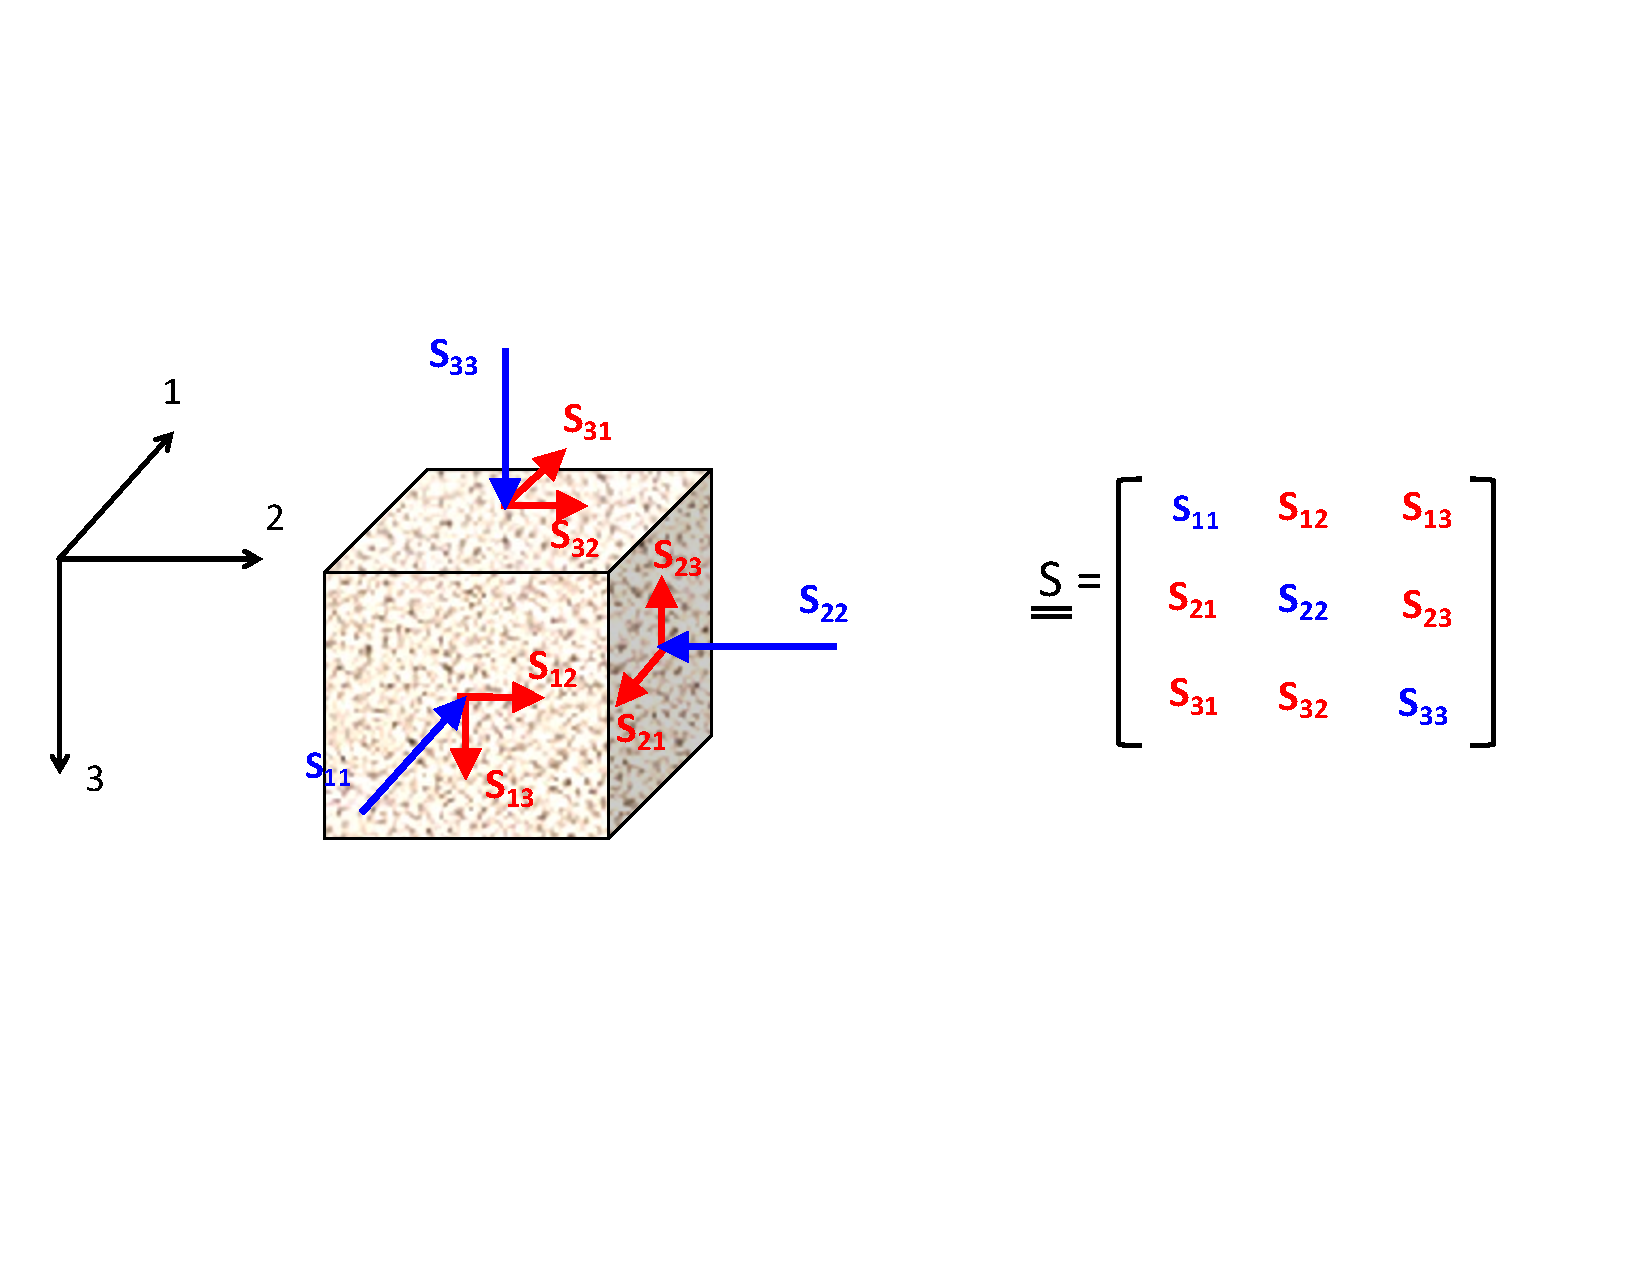
\includegraphics[scale=0.55]{.././Figures/split/4-3.pdf}%
\lthtmlpictureZ
\lthtmlcheckvsize\clearpage}

{\newpage\clearpage
\lthtmlinlinemathA{tex2html_wrap_inline15866}%
$ S_1 \geq S_2 \geq S_3$%
\lthtmlindisplaymathZ
\lthtmlcheckvsize\clearpage}

{\newpage\clearpage
\lthtmlpictureA{tex2html_wrap15870}%
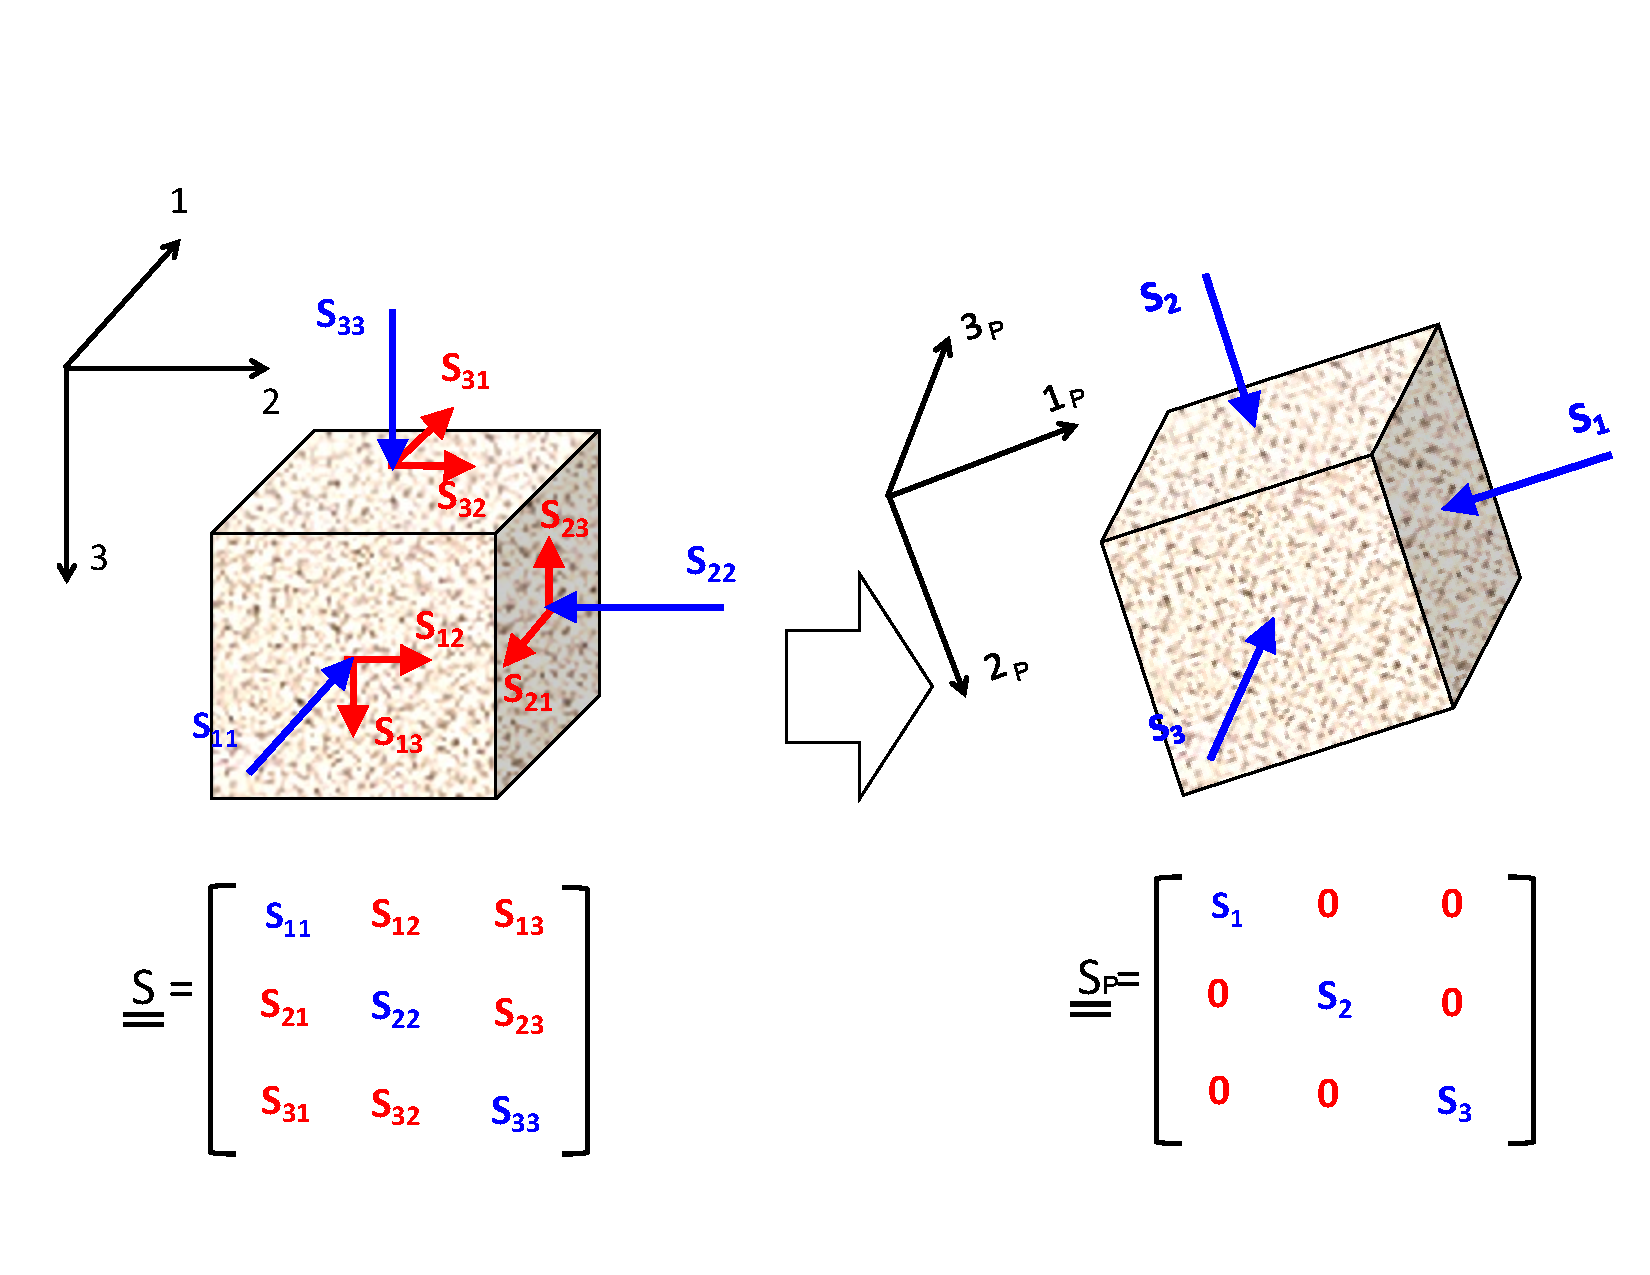
\includegraphics[scale=0.55]{.././Figures/split/4-4.pdf}%
\lthtmlpictureZ
\lthtmlcheckvsize\clearpage}

\stepcounter{subsection}
{\newpage\clearpage
\lthtmlinlinemathA{tex2html_wrap_inline15876}%
$ \uline{a}$%
\lthtmlindisplaymathZ
\lthtmlcheckvsize\clearpage}

{\newpage\clearpage
\lthtmlinlinemathA{tex2html_wrap_inline15878}%
$ m \uline{a} = 0$%
\lthtmlindisplaymathZ
\lthtmlcheckvsize\clearpage}

{\newpage\clearpage
\lthtmlinlinemathA{tex2html_wrap_inline15880}%
$ \rho V b_1$%
\lthtmlindisplaymathZ
\lthtmlcheckvsize\clearpage}

{\newpage\clearpage
\lthtmlinlinemathA{tex2html_wrap_inline15882}%
$ \rho$%
\lthtmlindisplaymathZ
\lthtmlcheckvsize\clearpage}

{\newpage\clearpage
\lthtmlinlinemathA{tex2html_wrap_inline15884}%
$ V$%
\lthtmlindisplaymathZ
\lthtmlcheckvsize\clearpage}

{\newpage\clearpage
\lthtmlinlinemathA{tex2html_wrap_inline15886}%
$ b_1$%
\lthtmlindisplaymathZ
\lthtmlcheckvsize\clearpage}

{\newpage\clearpage
\lthtmldisplayA{displaymath15888}%
\begin{displaymath}\begin{array}{rcl}
\sum F_1 & = & 0 \\
\sum F_1 & =
& + S_{11} dx_2 dx_3 - \left[ S_{11} + (\frac{\partial S_{11}}{\partial x_1}) dx_1 \right] dx_2 dx_3 \\
& & + S_{21} dx_1 dx_3 - \left[ S_{21} + (\frac{\partial S_{21}}{\partial x_2}) dx_2 \right] dx_1 dx_3 \\
& & + S_{31} dx_1 dx_2 - \left[ S_{31} + (\frac{\partial S_{31}}{\partial x_3}) dx_3 \right] dx_1 dx_2 \\
& & - \rho (dx_1 dx_2 dx_3) b_1 = 0
\end{array}\end{displaymath}%
\lthtmldisplayZ
\lthtmlcheckvsize\clearpage}

{\newpage\clearpage
\lthtmlinlinemathA{tex2html_wrap_inline15890}%
$ (dx_1 dx_2 dx_3)$%
\lthtmlindisplaymathZ
\lthtmlcheckvsize\clearpage}

{\newpage\clearpage
\lthtmlinlinemathA{tex2html_wrap_indisplay15892}%
$\displaystyle \frac{\partial S_{11}}{\partial x_1} +
\frac{\partial S_{21}}{\partial x_2} +
\frac{\partial S_{31}}{\partial x_3} -
\rho b_1 = 0$%
\lthtmlindisplaymathZ
\lthtmlcheckvsize\clearpage}

{\newpage\clearpage
\lthtmlpictureA{tex2html_wrap15894}%
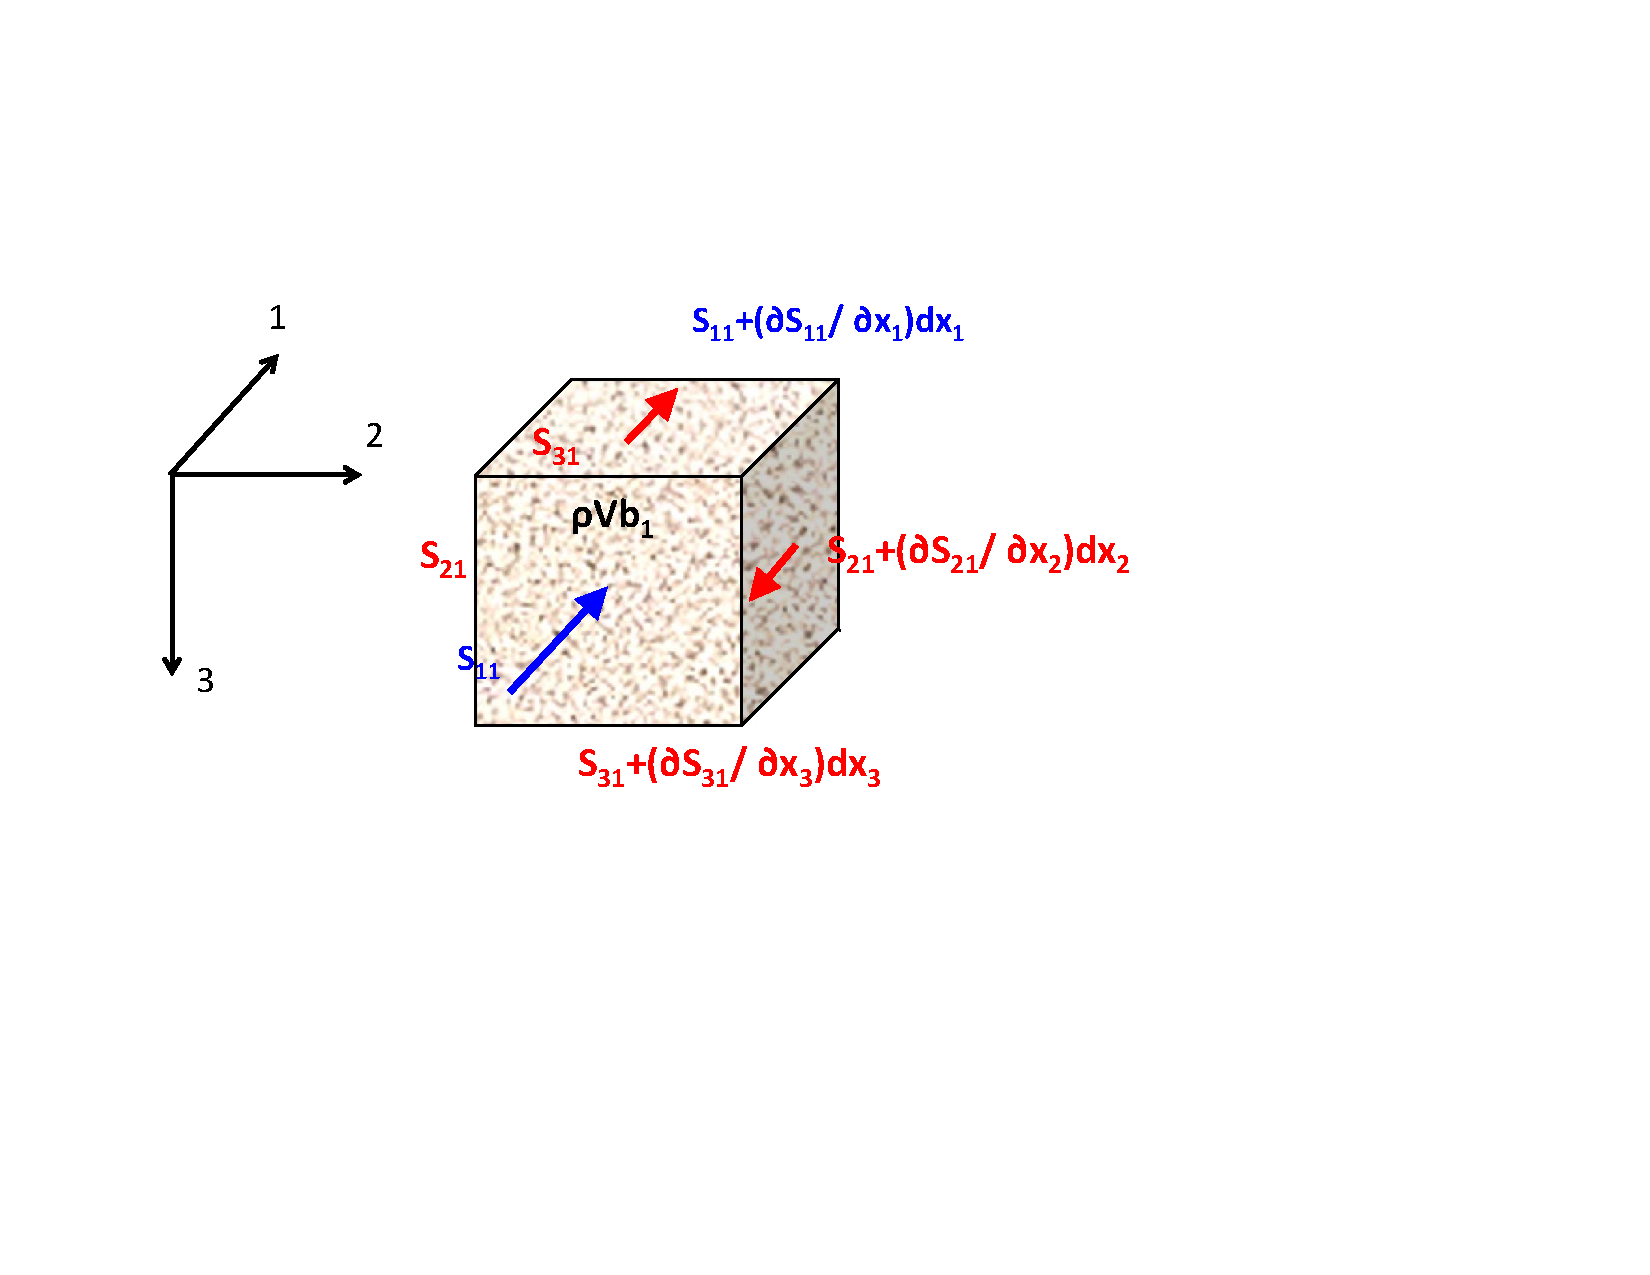
\includegraphics[scale=0.65]{.././Figures/split/4-5.pdf}%
\lthtmlpictureZ
\lthtmlcheckvsize\clearpage}

{\newpage\clearpage
\lthtmldisplayA{displaymath15911}%
\begin{displaymath}\displaystyle
\left\lbrace
\begin{array}{rcl}
\cfrac{\partial S_{11}}{\partial x_1} +
\cfrac{\partial S_{21}}{\partial x_2} +
\cfrac{\partial S_{31}}{\partial x_3} -
\rho b_1 & = & 0 \\
\cfrac{\partial S_{12}}{\partial x_1} +
\cfrac{\partial S_{22}}{\partial x_2} +
\cfrac{\partial S_{33}}{\partial x_3} -
\rho b_2 & = & 0 \\
\cfrac{\partial S_{13}}{\partial x_1} +
\cfrac{\partial S_{23}}{\partial x_2} +
\cfrac{\partial S_{33}}{\partial x_3} -
\rho b_3 & = & 0 \\
\end{array}
\right.\end{displaymath}%
\lthtmldisplayZ
\lthtmlcheckvsize\clearpage}

\stepcounter{subsection}
{\newpage\clearpage
\lthtmlinlinemathA{tex2html_wrap_inline15914}%
$ g$%
\lthtmlindisplaymathZ
\lthtmlcheckvsize\clearpage}

{\newpage\clearpage
\lthtmlinlinemathA{tex2html_wrap_inline15916}%
$ b_3 = g$%
\lthtmlindisplaymathZ
\lthtmlcheckvsize\clearpage}

{\newpage\clearpage
\lthtmlinlinemathA{tex2html_wrap_inline15918}%
$ \partial()/\partial x_1 = \partial()/\partial x_2 = 0$%
\lthtmlindisplaymathZ
\lthtmlcheckvsize\clearpage}

{\newpage\clearpage
\lthtmlinlinemathA{tex2html_wrap_indisplay15924}%
$\displaystyle S_{33}(x_3) = \int_0^{x_3} \rho(x_3) g \: dx_3$%
\lthtmlindisplaymathZ
\lthtmlcheckvsize\clearpage}

{\newpage\clearpage
\lthtmlpictureA{tex2html_wrap15926}%
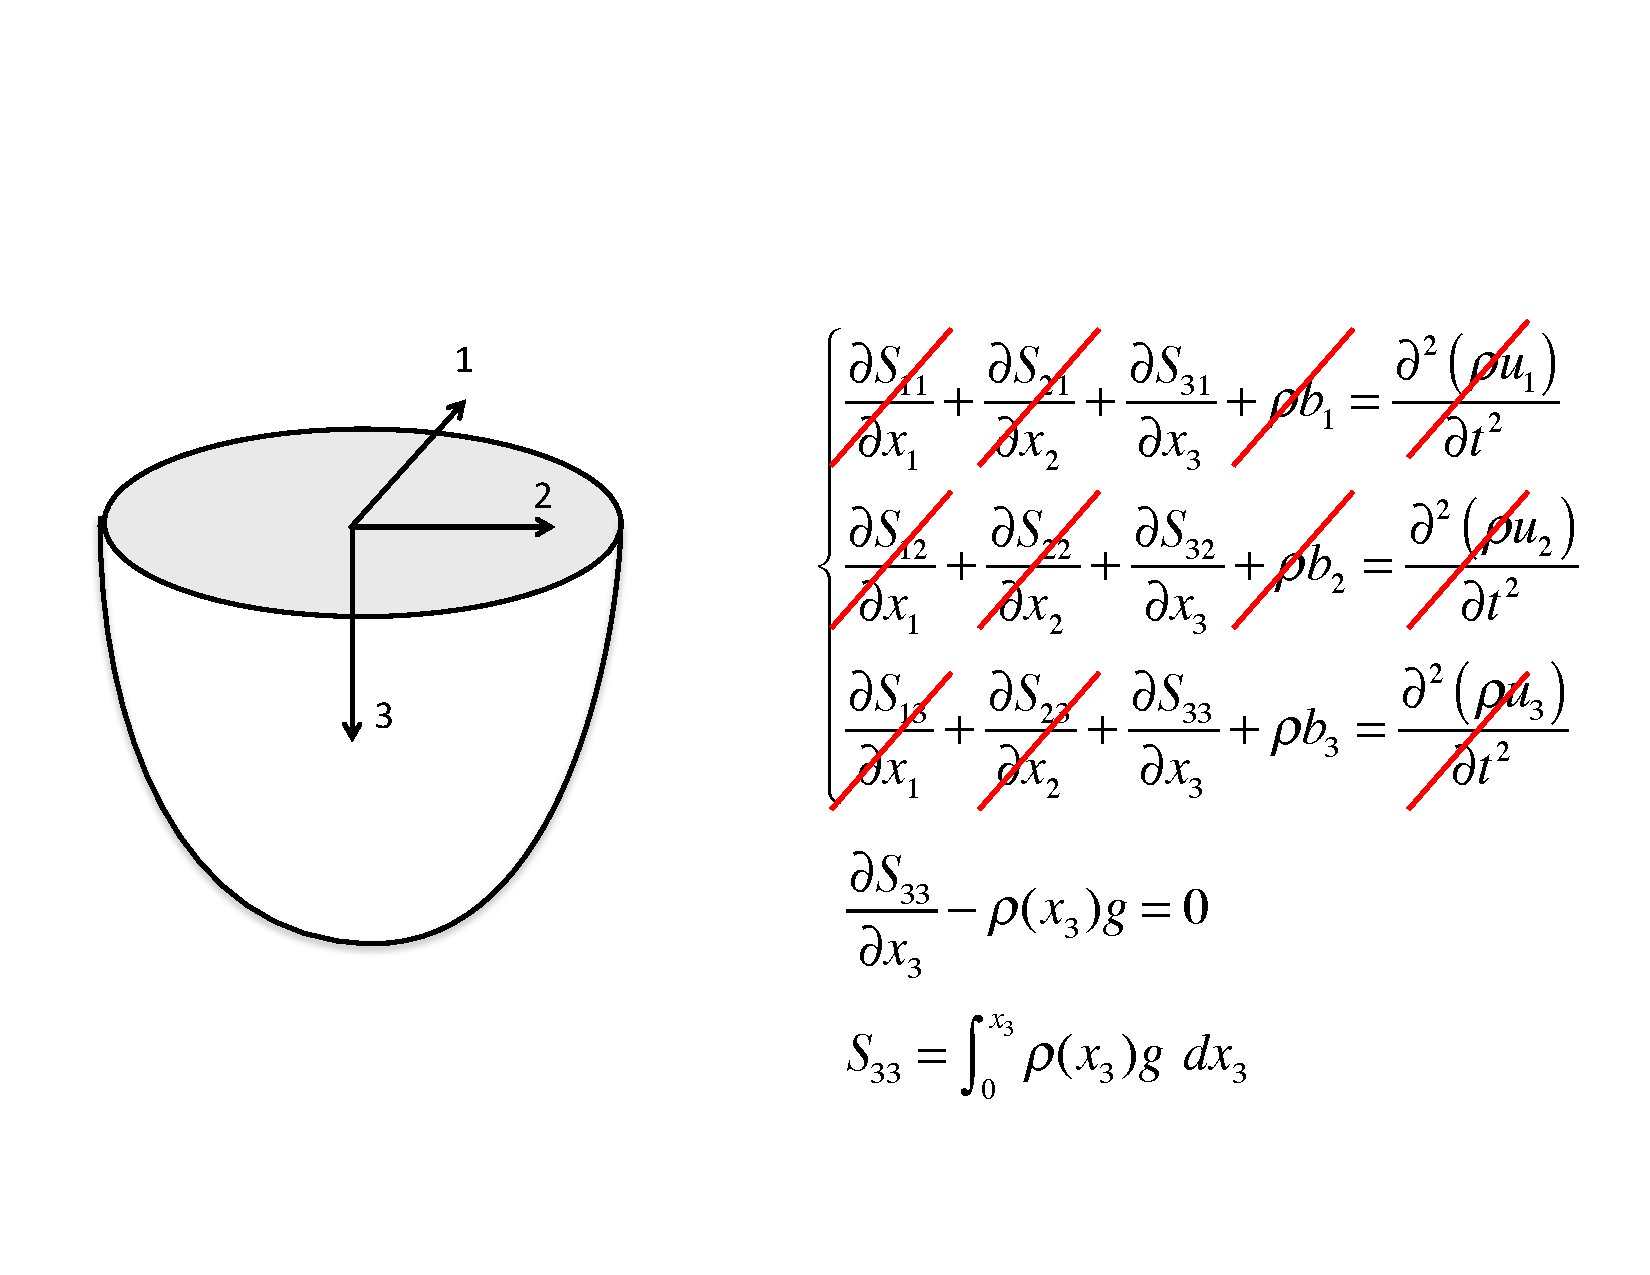
\includegraphics[scale=0.45]{.././Figures/split/4-7.pdf}%
\lthtmlpictureZ
\lthtmlcheckvsize\clearpage}

{\newpage\clearpage
\lthtmlinlinemathA{tex2html_wrap_inline15935}%
$ S_{11}$%
\lthtmlindisplaymathZ
\lthtmlcheckvsize\clearpage}

{\newpage\clearpage
\lthtmlinlinemathA{tex2html_wrap_inline15937}%
$ S_{22}$%
\lthtmlindisplaymathZ
\lthtmlcheckvsize\clearpage}

\stepcounter{subsection}
{\newpage\clearpage
\lthtmlinlinemathA{tex2html_wrap_inline15940}%
$ \uline{t}$%
\lthtmlindisplaymathZ
\lthtmlcheckvsize\clearpage}

{\newpage\clearpage
\lthtmlinlinemathA{tex2html_wrap_inline15944}%
$ \uline{b}$%
\lthtmlindisplaymathZ
\lthtmlcheckvsize\clearpage}

{\newpage\clearpage
\lthtmlpictureA{tex2html_wrap15946}%
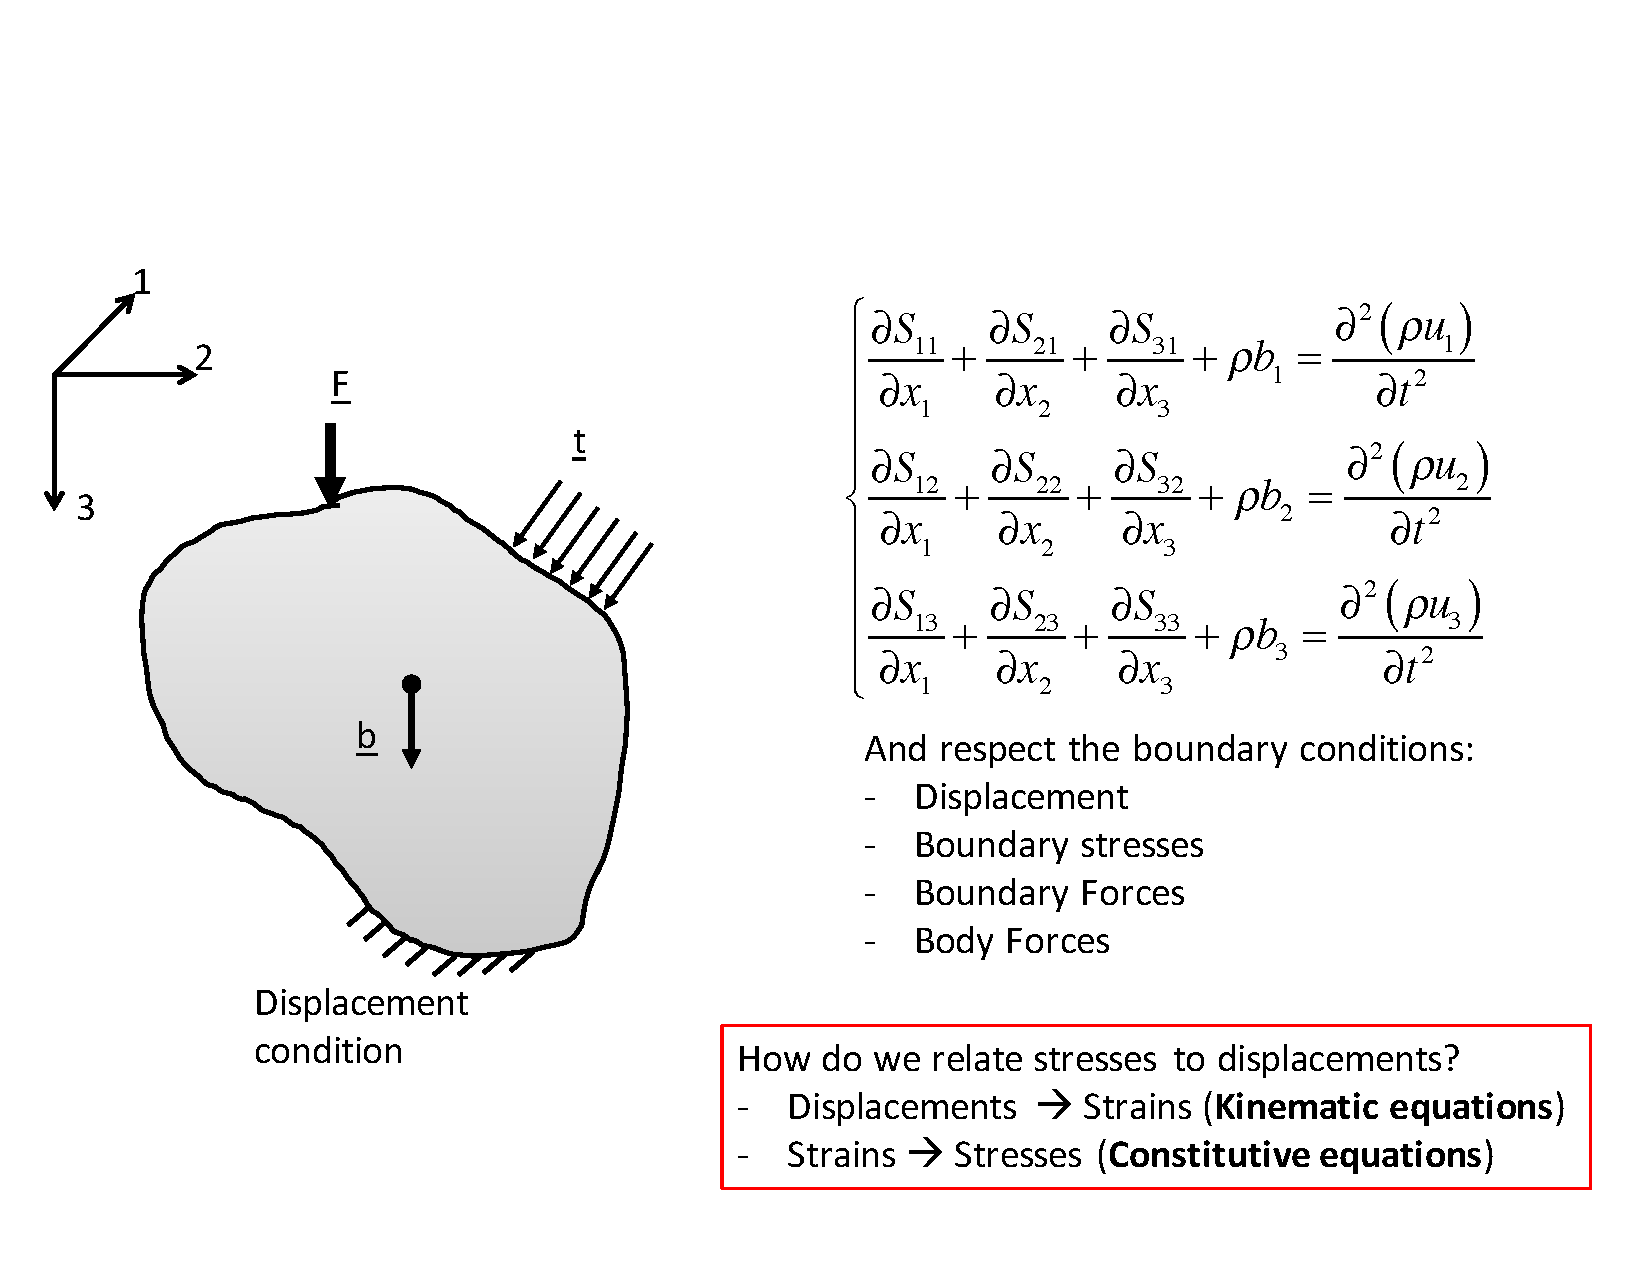
\includegraphics[scale=0.55]{.././Figures/split/4-8.pdf}%
\lthtmlpictureZ
\lthtmlcheckvsize\clearpage}

\stepcounter{section}
{\newpage\clearpage
\lthtmlpictureA{tex2html_wrap15952}%
\includegraphics[scale=0.65]{.././Figures/split/4-9.pdf}%
\lthtmlpictureZ
\lthtmlcheckvsize\clearpage}

{\newpage\clearpage
\lthtmlinlinemathA{tex2html_wrap_indisplay15959}%
$\displaystyle \varepsilon_{11} = \frac{\Delta u_1}{\Delta x_1}$%
\lthtmlindisplaymathZ
\lthtmlcheckvsize\clearpage}

{\newpage\clearpage
\lthtmlinlinemathA{tex2html_wrap_indisplay15961}%
$\displaystyle \varepsilon_{22} = \frac{\Delta u_2}{\Delta x_2}$%
\lthtmlindisplaymathZ
\lthtmlcheckvsize\clearpage}

{\newpage\clearpage
\lthtmlinlinemathA{tex2html_wrap_inline15963}%
$ \pi - \left[ \pi - \arctan(\Delta u_1 / \Delta x_2) + \arctan(\Delta u_2 / \Delta x_1) \right] $%
\lthtmlindisplaymathZ
\lthtmlcheckvsize\clearpage}

{\newpage\clearpage
\lthtmlinlinemathA{tex2html_wrap_inline15965}%
$ \arctan(x/y) \sim x/y$%
\lthtmlindisplaymathZ
\lthtmlcheckvsize\clearpage}

{\newpage\clearpage
\lthtmlinlinemathA{tex2html_wrap_indisplay15967}%
$\displaystyle \varepsilon_{12} = \frac{1}{2} \left( \frac{\Delta u_1}{\Delta x_2} + \frac{\Delta u_2}{\Delta x_1} \right)$%
\lthtmlindisplaymathZ
\lthtmlcheckvsize\clearpage}

{\newpage\clearpage
\lthtmlpictureA{tex2html_wrap15969}%
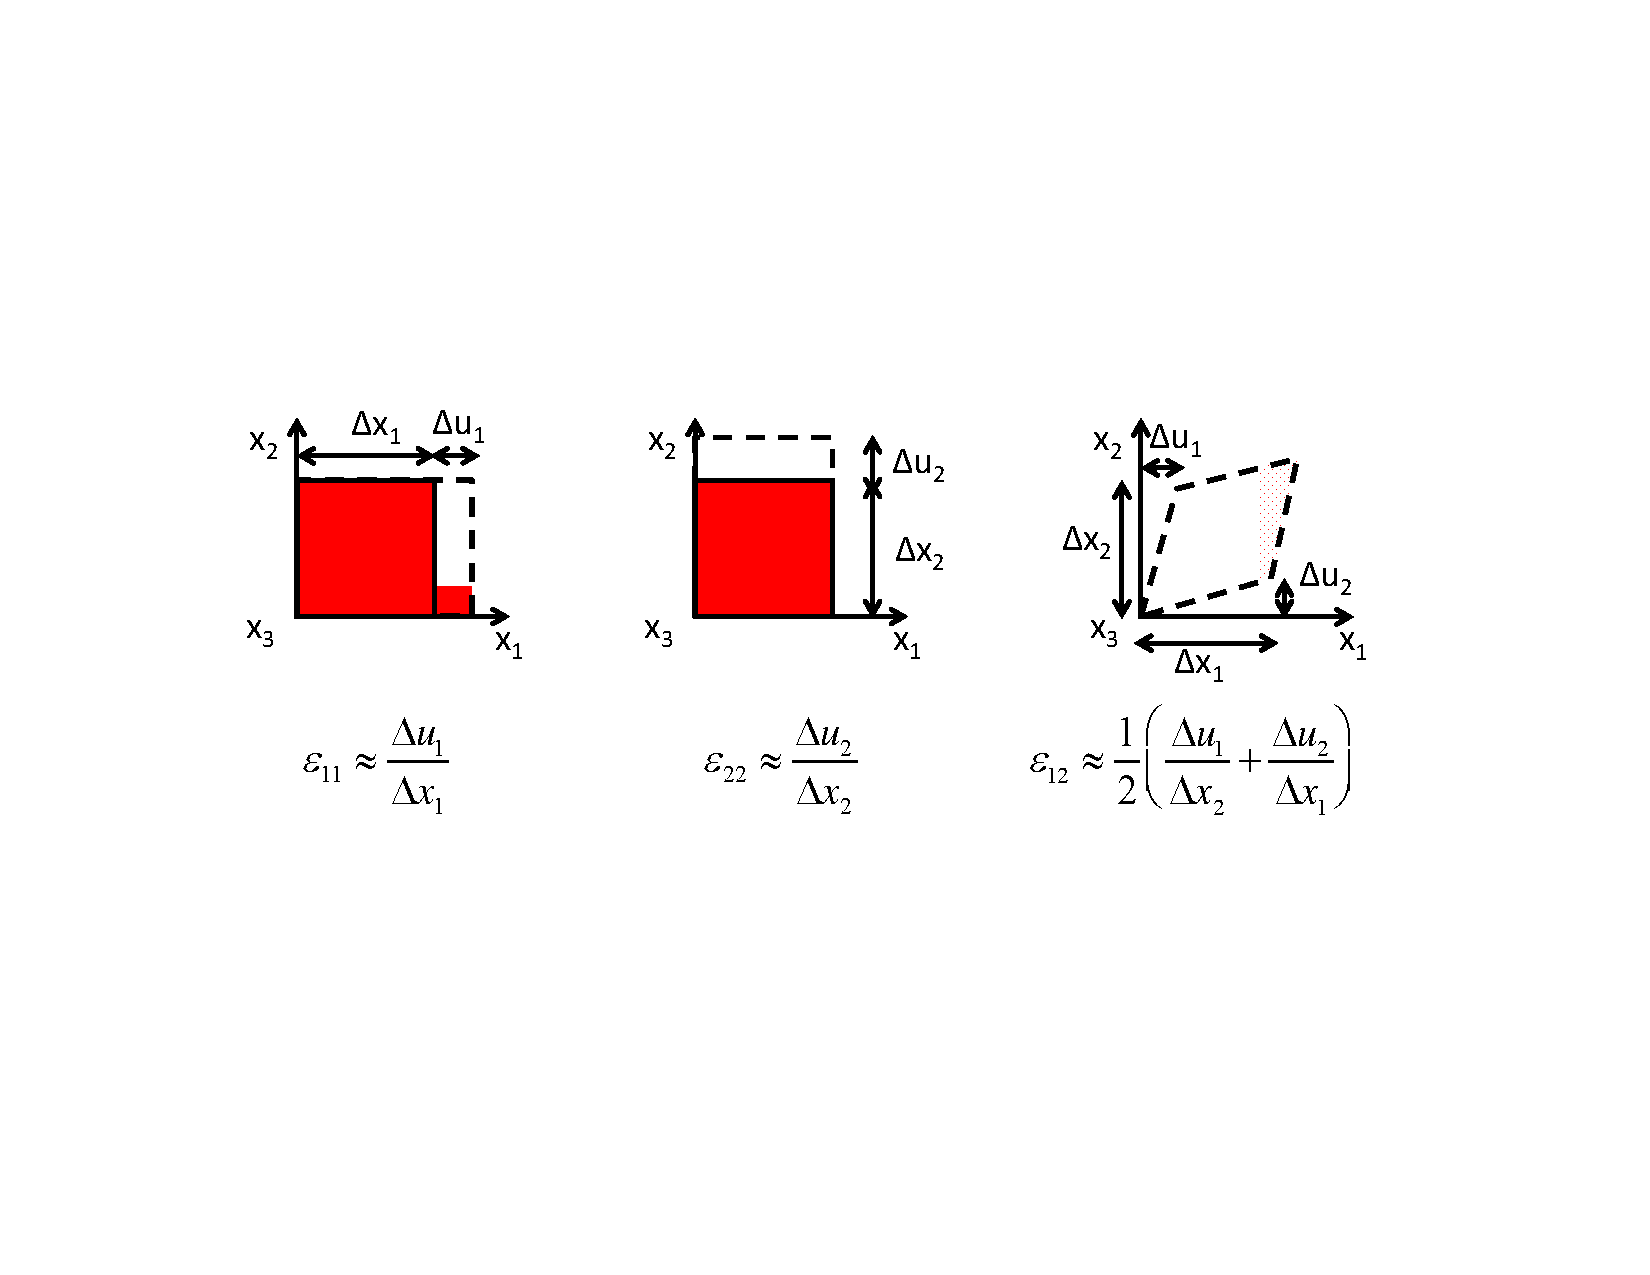
\includegraphics[scale=0.65]{.././Figures/split/4-10.pdf}%
\lthtmlpictureZ
\lthtmlcheckvsize\clearpage}

{\newpage\clearpage
\lthtmlinlinemathA{tex2html_wrap_inline15974}%
$ x_i$%
\lthtmlindisplaymathZ
\lthtmlcheckvsize\clearpage}

{\newpage\clearpage
\lthtmldisplayA{displaymath15976}%
\begin{displaymath}\uuline{\varepsilon} =
\left[
\begin{array}{ccc}
\cfrac{\partial u_1}{\partial x_1} & \cfrac{1}{2} \left( \cfrac{\partial u_1}{\partial x_2} + \cfrac{\partial u_2}{\partial x_1} \right) &  \cfrac{1}{2} \left( \cfrac{\partial u_1}{\partial x_3} + \cfrac{\partial u_3}{\partial x_1} \right)\\
\cfrac{1}{2} \left( \cfrac{\partial u_2}{\partial x_1} + \cfrac{\partial u_1}{\partial x_2} \right) & \cfrac{\partial u_2}{\partial x_2} & \cfrac{1}{2} \left( \cfrac{\partial u_2}{\partial x_3} + \cfrac{\partial u_3}{\partial x_2} \right)\\
\cfrac{1}{2} \left( \cfrac{\partial u_3}{\partial x_1} + \cfrac{\partial u_1}{\partial x_3} \right) &  \cfrac{1}{2} \left( \cfrac{\partial u_3}{\partial x_2} + \cfrac{\partial u_2}{\partial x_3} \right) & \cfrac{\partial u_3}{\partial x_3}
\end{array}
\right] =
\left[
\begin{array}{ccc}
\varepsilon_{11} & \varepsilon_{12}  &  \varepsilon_{13} \\
\varepsilon_{21} & \varepsilon_{22}  &  \varepsilon_{23} \\
\varepsilon_{31} & \varepsilon_{32}  &  \varepsilon_{33}
\end{array}
\right]\end{displaymath}%
\lthtmldisplayZ
\lthtmlcheckvsize\clearpage}

{\newpage\clearpage
\lthtmlinlinemathA{tex2html_wrap_indisplay15978}%
$\displaystyle \varepsilon_{vol} = \varepsilon_{11} + \varepsilon_{22} + \varepsilon_{33}$%
\lthtmlindisplaymathZ
\lthtmlcheckvsize\clearpage}

{\newpage\clearpage
\lthtmlinlinemathA{tex2html_wrap_inline15980}%
$ \Delta x_1 \Delta x_2 \Delta x_3$%
\lthtmlindisplaymathZ
\lthtmlcheckvsize\clearpage}

{\newpage\clearpage
\lthtmlinlinemathA{tex2html_wrap_inline15982}%
$ \Delta V$%
\lthtmlindisplaymathZ
\lthtmlcheckvsize\clearpage}

{\newpage\clearpage
\lthtmlinlinemathA{tex2html_wrap_inline15984}%
$ V_0$%
\lthtmlindisplaymathZ
\lthtmlcheckvsize\clearpage}

{\newpage\clearpage
\lthtmlinlinemathA{tex2html_wrap_indisplay15986}%
$\displaystyle \varepsilon_{vol} =  \frac{\Delta V}{V_0}
$%
\lthtmlindisplaymathZ
\lthtmlcheckvsize\clearpage}

{\newpage\clearpage
\lthtmlinlinemathA{tex2html_wrap_inline15988}%
$ \mathrm{d} x_1 \mathrm{d} x_2 \mathrm{d} x_3$%
\lthtmlindisplaymathZ
\lthtmlcheckvsize\clearpage}

{\newpage\clearpage
\lthtmlinlinemathA{tex2html_wrap_inline15990}%
$ (\mathrm{d} x_1 + \mathrm{d}u_1)(\mathrm{d} u_2 + \mathrm{d}u_2)(\mathrm{d} x_3 + \mathrm{d} u_3)$%
\lthtmlindisplaymathZ
\lthtmlcheckvsize\clearpage}

{\newpage\clearpage
\lthtmlinlinemathA{tex2html_wrap_indisplay15992}%
$\displaystyle \varepsilon_{vol} =  \frac{[(\mathrm{d} x_1 + \mathrm{d}u_1)(\mathrm{d} x_2 + \mathrm{d}u_2)(\mathrm{d} x_3 + \mathrm{d}u_3) - (\mathrm{d} x_1 \mathrm{d} x_2 \mathrm{d} x_3)]}{(\mathrm{d} x_1 \mathrm{d} x_2 \mathrm{d} x_3)}
$%
\lthtmlindisplaymathZ
\lthtmlcheckvsize\clearpage}

{\newpage\clearpage
\lthtmlinlinemathA{tex2html_wrap_inline15994}%
$ \mathrm{d}u_i \mathrm{d}u_j$%
\lthtmlindisplaymathZ
\lthtmlcheckvsize\clearpage}

{\newpage\clearpage
\lthtmlinlinemathA{tex2html_wrap_inline15996}%
$ \mathrm{d}u_1 \mathrm{d}u_2 \mathrm{d}u_3$%
\lthtmlindisplaymathZ
\lthtmlcheckvsize\clearpage}

{\newpage\clearpage
\lthtmlinlinemathA{tex2html_wrap_inline15998}%
$ \mathrm{d}u_i$%
\lthtmlindisplaymathZ
\lthtmlcheckvsize\clearpage}

{\newpage\clearpage
\lthtmlinlinemathA{tex2html_wrap_inline16000}%
$ \mathrm{d}u_i << \mathrm{d}x_j $%
\lthtmlindisplaymathZ
\lthtmlcheckvsize\clearpage}

{\newpage\clearpage
\lthtmlinlinemathA{tex2html_wrap_indisplay16002}%
$\displaystyle \varepsilon_{vol} \sim  \frac{(\mathrm{d} x_1 \mathrm{d} x_2 \mathrm{d}u_3 + 
							 \mathrm{d} x_1 \mathrm{d} x_3 \mathrm{d}u_2 +
							 \mathrm{d} x_2 \mathrm{d} x_3 \mathrm{d}u_1)}
							 {(\mathrm{d} x_1 \mathrm{d} x_2 \mathrm{d} x_3)}
				=  \frac{\mathrm{d}u_1}{\mathrm{d} x_1} + 
				   \frac{\mathrm{d}u_2}{\mathrm{d} x_2} + 
				   \frac{\mathrm{d}u_3}{\mathrm{d} x_3} 
				= \varepsilon_{11} + \varepsilon_{22} + \varepsilon_{33} \: \: \blacksquare
$%
\lthtmlindisplaymathZ
\lthtmlcheckvsize\clearpage}

\stepcounter{section}
{\newpage\clearpage
\lthtmlpictureA{tex2html_wrap16005}%
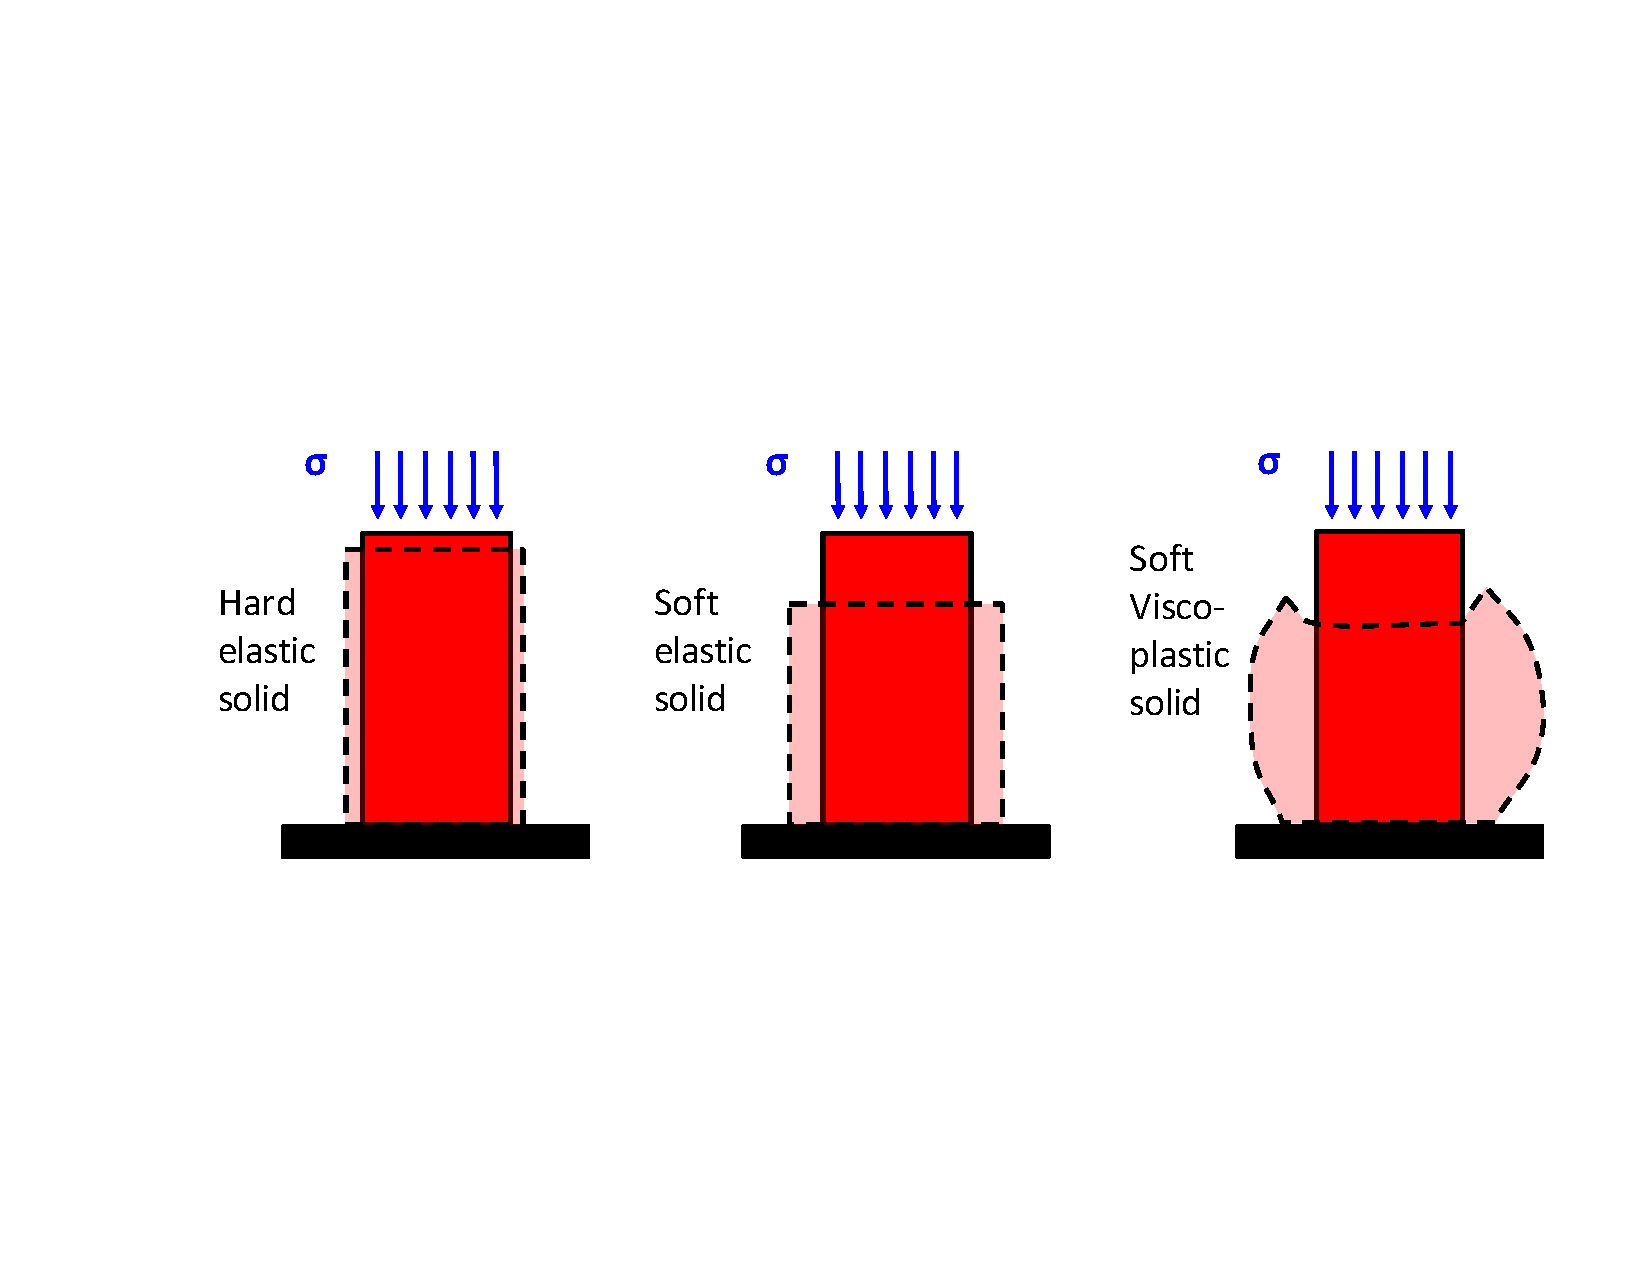
\includegraphics[scale=0.65]{.././Figures/split/4-12.pdf}%
\lthtmlpictureZ
\lthtmlcheckvsize\clearpage}

{\newpage\clearpage
\lthtmlinlinemathA{tex2html_wrap_inline16010}%
$ F$%
\lthtmlindisplaymathZ
\lthtmlcheckvsize\clearpage}

{\newpage\clearpage
\lthtmlinlinemathA{tex2html_wrap_inline16012}%
$ \Delta x$%
\lthtmlindisplaymathZ
\lthtmlcheckvsize\clearpage}

{\newpage\clearpage
\lthtmlinlinemathA{tex2html_wrap_indisplay16016}%
$\displaystyle F = k \Delta x$%
\lthtmlindisplaymathZ
\lthtmlcheckvsize\clearpage}

{\newpage\clearpage
\lthtmlinlinemathA{tex2html_wrap_inline16028}%
$ E$%
\lthtmlindisplaymathZ
\lthtmlcheckvsize\clearpage}

{\newpage\clearpage
\lthtmlinlinemathA{tex2html_wrap_indisplay16030}%
$\displaystyle \frac{F}{A} = E \frac{\Delta x}{L}$%
\lthtmlindisplaymathZ
\lthtmlcheckvsize\clearpage}

{\newpage\clearpage
\lthtmlinlinemathA{tex2html_wrap_inline16032}%
$ \sigma$%
\lthtmlindisplaymathZ
\lthtmlcheckvsize\clearpage}

{\newpage\clearpage
\lthtmlinlinemathA{tex2html_wrap_inline16034}%
$ \varepsilon$%
\lthtmlindisplaymathZ
\lthtmlcheckvsize\clearpage}

{\newpage\clearpage
\lthtmlinlinemathA{tex2html_wrap_indisplay16036}%
$\displaystyle \sigma = E \varepsilon$%
\lthtmlindisplaymathZ
\lthtmlcheckvsize\clearpage}

{\newpage\clearpage
\lthtmlinlinemathA{tex2html_wrap_inline16038}%
$ \uuline{\sigma}$%
\lthtmlindisplaymathZ
\lthtmlcheckvsize\clearpage}

{\newpage\clearpage
\lthtmlinlinemathA{tex2html_wrap_inline16040}%
$ \uuline{\varepsilon}$%
\lthtmlindisplaymathZ
\lthtmlcheckvsize\clearpage}

{\newpage\clearpage
\lthtmlinlinemathA{tex2html_wrap_inline16042}%
$ \uuline{C}$%
\lthtmlindisplaymathZ
\lthtmlcheckvsize\clearpage}

{\newpage\clearpage
\lthtmlinlinemathA{tex2html_wrap_indisplay16044}%
$\displaystyle \uuline{\sigma} = \uuline{C} \: \uuline{\varepsilon}$%
\lthtmlindisplaymathZ
\lthtmlcheckvsize\clearpage}

{\newpage\clearpage
\lthtmlpictureA{tex2html_wrap16046}%
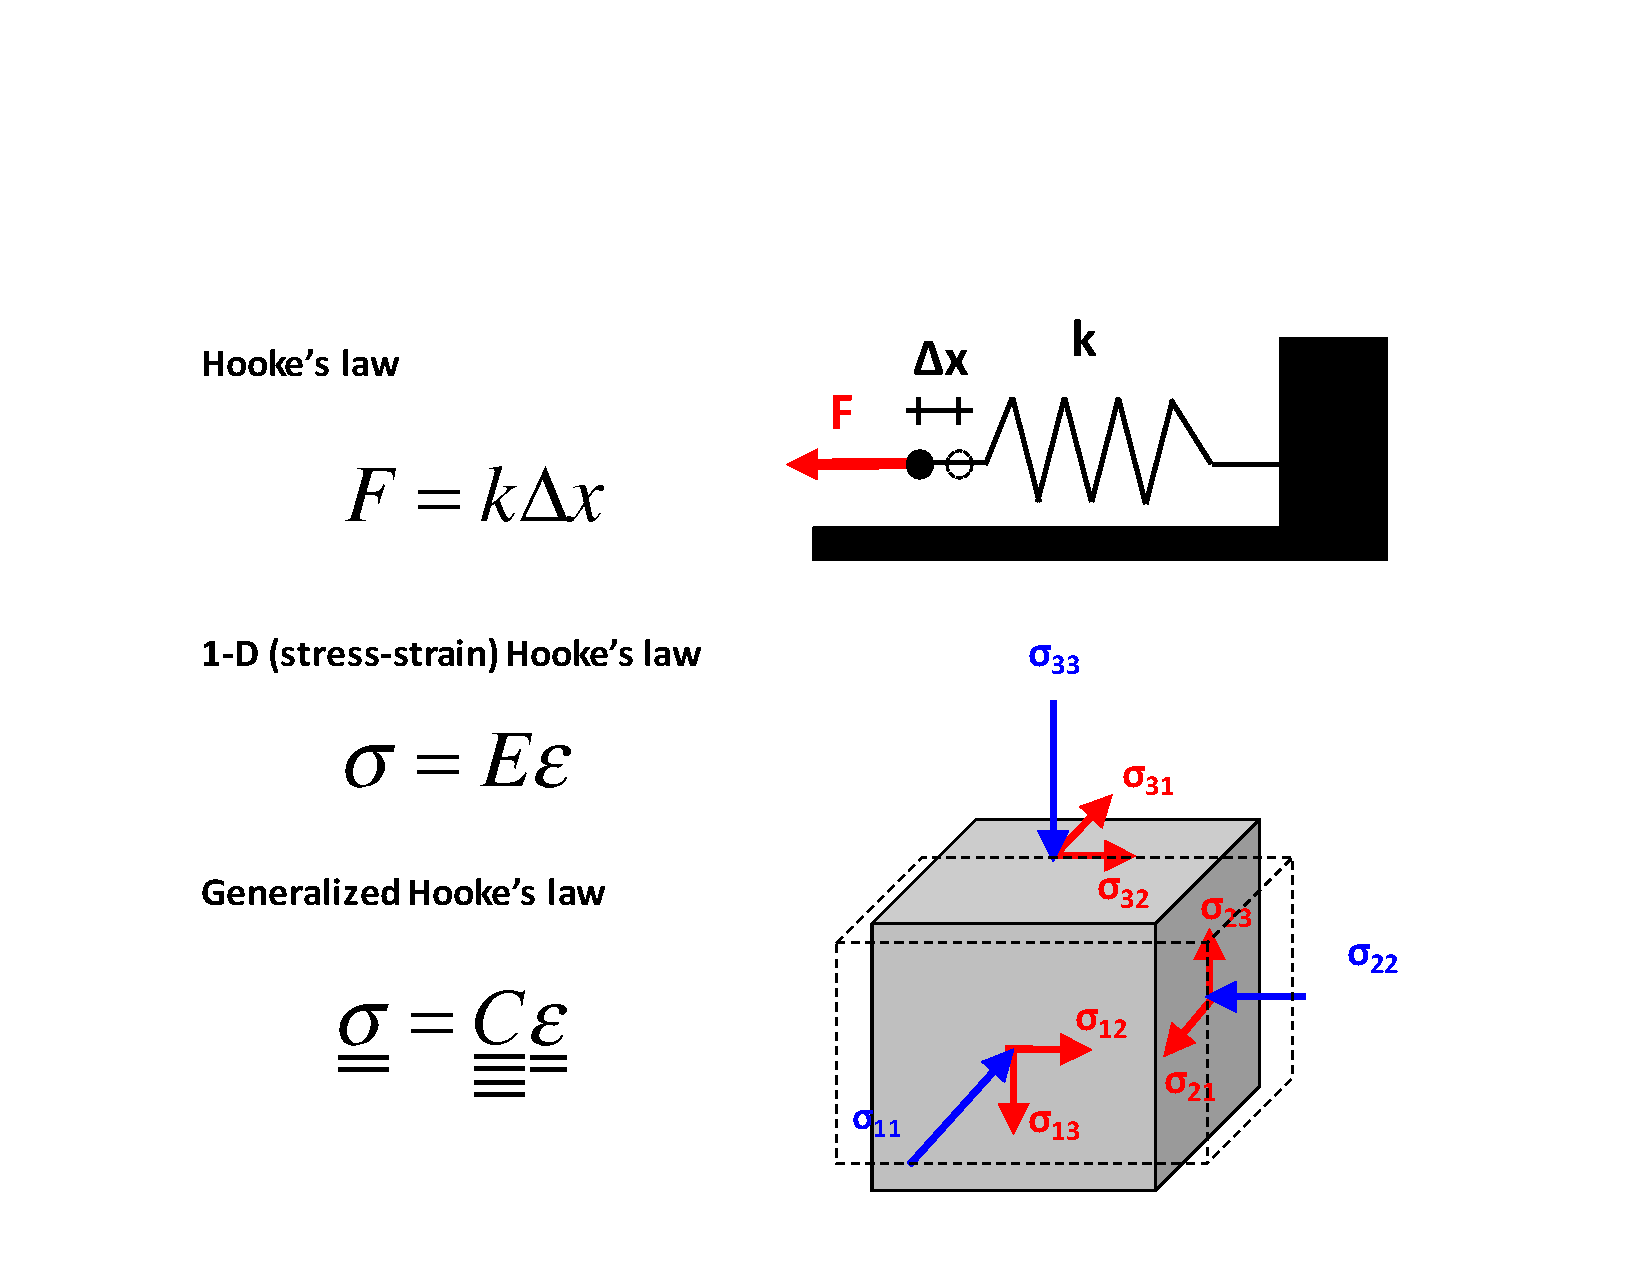
\includegraphics[scale=0.50]{.././Figures/split/4-13.pdf}%
\lthtmlpictureZ
\lthtmlcheckvsize\clearpage}

\stepcounter{subsection}
{\newpage\clearpage
\lthtmlinlinemathA{tex2html_wrap_inline16054}%
$ \sigma_{33}$%
\lthtmlindisplaymathZ
\lthtmlcheckvsize\clearpage}

{\newpage\clearpage
\lthtmlinlinemathA{tex2html_wrap_inline16060}%
$ \varepsilon_{33}$%
\lthtmlindisplaymathZ
\lthtmlcheckvsize\clearpage}

{\newpage\clearpage
\lthtmlinlinemathA{tex2html_wrap_indisplay16062}%
$\displaystyle E = \frac{\sigma_{33}}{\varepsilon_{33}}$%
\lthtmlindisplaymathZ
\lthtmlcheckvsize\clearpage}

{\newpage\clearpage
\lthtmlinlinemathA{tex2html_wrap_inline16064}%
$ \varepsilon_{11}$%
\lthtmlindisplaymathZ
\lthtmlcheckvsize\clearpage}

{\newpage\clearpage
\lthtmlinlinemathA{tex2html_wrap_inline16066}%
$ \varepsilon_{22}$%
\lthtmlindisplaymathZ
\lthtmlcheckvsize\clearpage}

{\newpage\clearpage
\lthtmlinlinemathA{tex2html_wrap_indisplay16070}%
$\displaystyle \nu = -\frac{\varepsilon_{11}}{\varepsilon_{33}}$%
\lthtmlindisplaymathZ
\lthtmlcheckvsize\clearpage}

{\newpage\clearpage
\lthtmlpictureA{tex2html_wrap16072}%
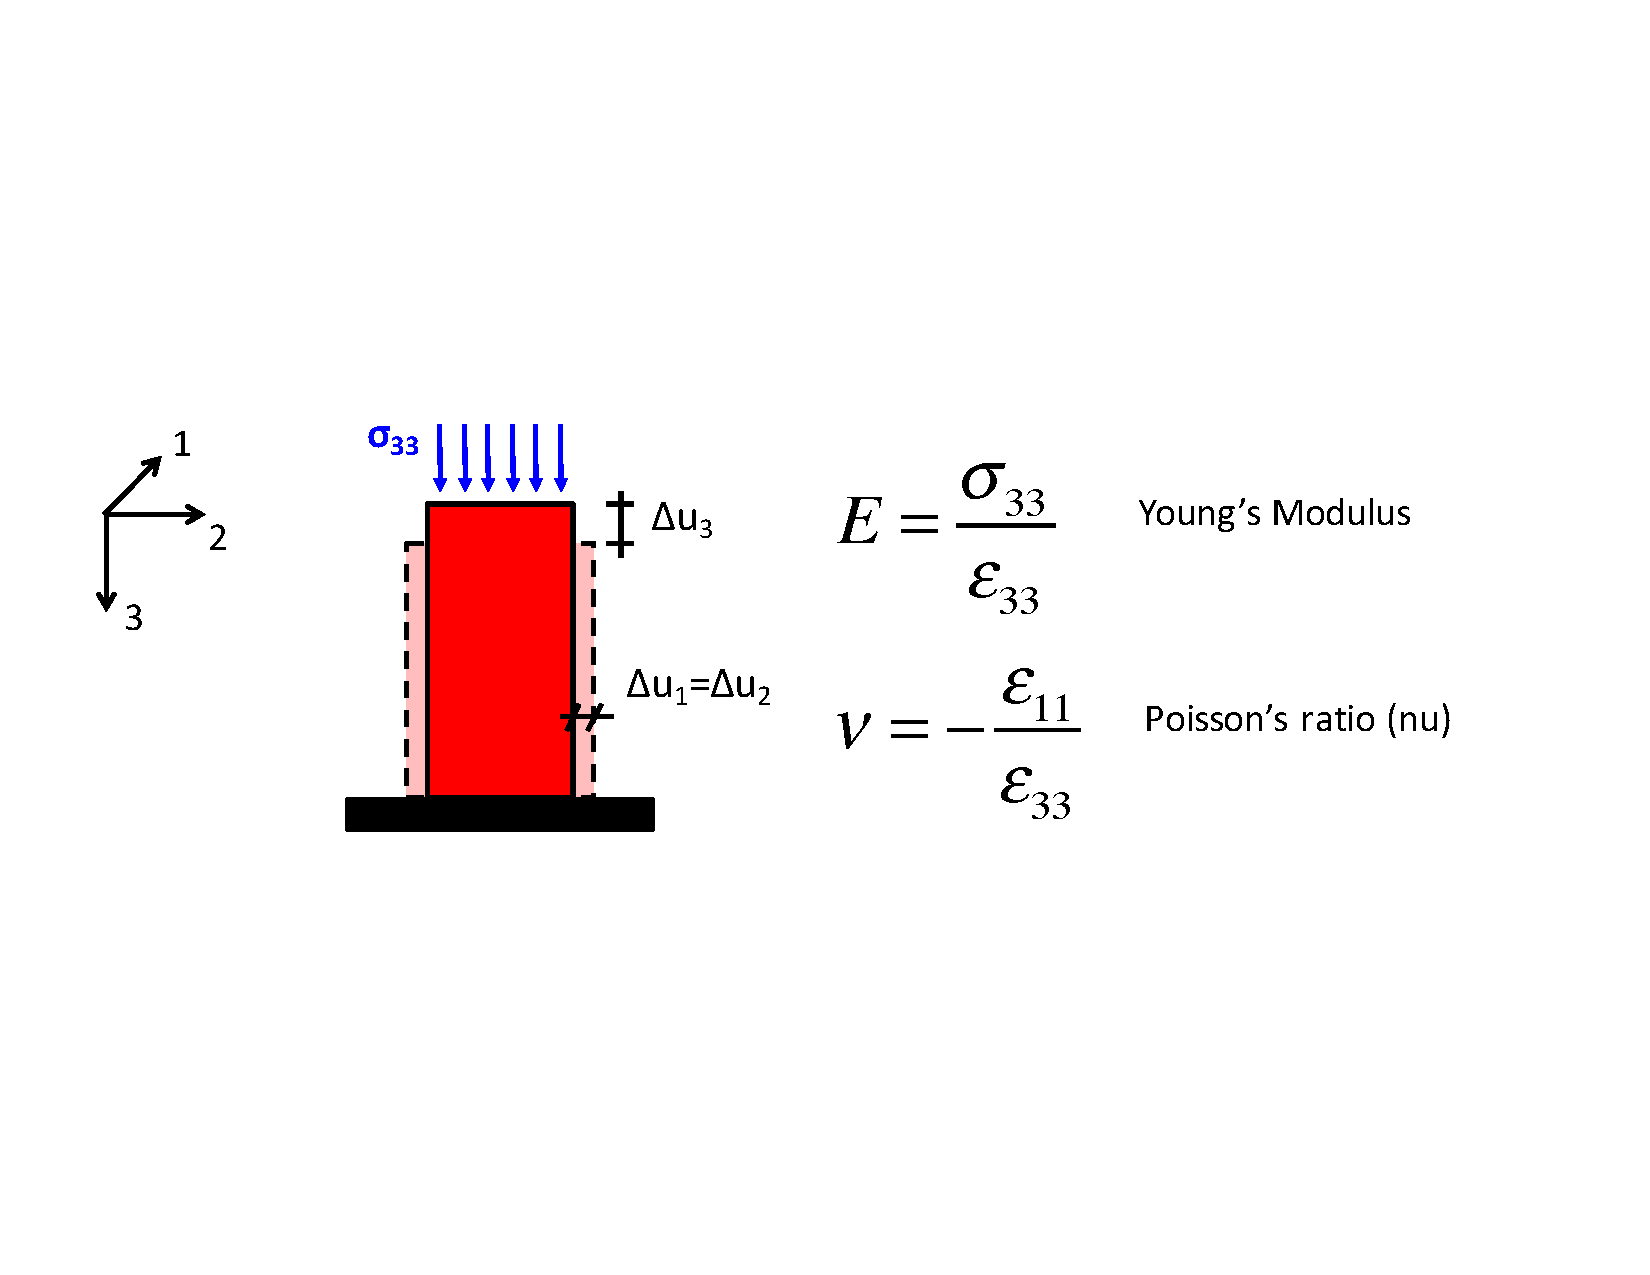
\includegraphics[scale=0.65]{.././Figures/split/4-14.pdf}%
\lthtmlpictureZ
\lthtmlcheckvsize\clearpage}

{\newpage\clearpage
\lthtmlinlinemathA{tex2html_wrap_inline16077}%
$ \sigma_a$%
\lthtmlindisplaymathZ
\lthtmlcheckvsize\clearpage}

{\newpage\clearpage
\lthtmlinlinemathA{tex2html_wrap_inline16079}%
$ \varepsilon_a$%
\lthtmlindisplaymathZ
\lthtmlcheckvsize\clearpage}

{\newpage\clearpage
\lthtmlinlinemathA{tex2html_wrap_indisplay16087}%
$\displaystyle \sigma_a = 3000$%
\lthtmlindisplaymathZ
\lthtmlcheckvsize\clearpage}

{\newpage\clearpage
\lthtmlinlinemathA{tex2html_wrap_indisplay16088}%
$\displaystyle = 3000 \frac{1}{145}$%
\lthtmlindisplaymathZ
\lthtmlcheckvsize\clearpage}

{\newpage\clearpage
\lthtmlinlinemathA{tex2html_wrap_indisplay16089}%
$\displaystyle = 20.7$%
\lthtmlindisplaymathZ
\lthtmlcheckvsize\clearpage}

{\newpage\clearpage
\lthtmlinlinemathA{tex2html_wrap_indisplay16091}%
$\displaystyle \varepsilon_a(1$%
\lthtmlindisplaymathZ
\lthtmlcheckvsize\clearpage}

{\newpage\clearpage
\lthtmlinlinemathA{tex2html_wrap_indisplay16092}%
$\displaystyle ) = \frac{\sigma_a}{E} = \frac{20.7 \text{ MPa}}{1000 \text{ MPa}} = 0.0207 = 2.07 \%
$%
\lthtmlindisplaymathZ
\lthtmlcheckvsize\clearpage}

{\newpage\clearpage
\lthtmlinlinemathA{tex2html_wrap_indisplay16094}%
$\displaystyle \varepsilon_a(10$%
\lthtmlindisplaymathZ
\lthtmlcheckvsize\clearpage}

{\newpage\clearpage
\lthtmlinlinemathA{tex2html_wrap_indisplay16095}%
$\displaystyle ) = \frac{\sigma_a}{E} = \frac{20.7 \text{ MPa}}{10000 \text{ MPa}} = 0.00207 = 0.207 \%
$%
\lthtmlindisplaymathZ
\lthtmlcheckvsize\clearpage}

{\newpage\clearpage
\lthtmlinlinemathA{tex2html_wrap_indisplay16097}%
$\displaystyle \varepsilon_a(50$%
\lthtmlindisplaymathZ
\lthtmlcheckvsize\clearpage}

{\newpage\clearpage
\lthtmlinlinemathA{tex2html_wrap_indisplay16098}%
$\displaystyle ) = \frac{\sigma_a}{E} = \frac{20.7 \text{ MPa}}{50000 \text{ MPa}} = 0.00041 = 0.041 \%
$%
\lthtmlindisplaymathZ
\lthtmlcheckvsize\clearpage}

\stepcounter{subsection}
{\newpage\clearpage
\lthtmldisplayA{displaymath16103}%
\begin{displaymath}\left\lbrace
\begin{array}{rcl}
\varepsilon_{11} & = & +\cfrac{1}{E} \: \sigma_{11} -\cfrac{\nu}{E} \: \sigma_{22} -\cfrac{\nu}{E} \: \sigma_{33}\\
\varepsilon_{22} & = &  -\cfrac{\nu}{E} \: \sigma_{11} +\cfrac{1}{E} \: \sigma_{22} - \cfrac{\nu}{E} \: \sigma_{33}\\
\varepsilon_{33} & = & -\cfrac{\nu}{E} \: \sigma_{11} -\cfrac{\nu}{E} \: \sigma_{22} + \cfrac{1}{E} \: \sigma_{33}
\end{array}
\right.\end{displaymath}%
\lthtmldisplayZ
\lthtmlcheckvsize\clearpage}

{\newpage\clearpage
\lthtmlinlinemathA{tex2html_wrap_inline16105}%
$ \varepsilon_{ij}$%
\lthtmlindisplaymathZ
\lthtmlcheckvsize\clearpage}

{\newpage\clearpage
\lthtmlinlinemathA{tex2html_wrap_inline16107}%
$ G=E/[2(1+\nu)]$%
\lthtmlindisplaymathZ
\lthtmlcheckvsize\clearpage}

{\newpage\clearpage
\lthtmldisplayA{displaymath16109}%
\begin{displaymath}\left\lbrace
\begin{array}{rcl}
2 \varepsilon_{12} & = & \cfrac{1}{G} \: \sigma_{12}\\
2 \varepsilon_{13} & = & \cfrac{1}{G} \: \sigma_{13}\\
2 \varepsilon_{23} & = & \cfrac{1}{G} \: \sigma_{23}
\end{array}
\right.\end{displaymath}%
\lthtmldisplayZ
\lthtmlcheckvsize\clearpage}

{\newpage\clearpage
\lthtmlinlinemathA{tex2html_wrap_inline16115}%
$ \uuline{D}$%
\lthtmlindisplaymathZ
\lthtmlcheckvsize\clearpage}

{\newpage\clearpage
\lthtmlinlinemathA{tex2html_wrap_indisplay16117}%
$\displaystyle \uuline{\varepsilon} = \uuline{D} \: \uuline{\sigma}$%
\lthtmlindisplaymathZ
\lthtmlcheckvsize\clearpage}

{\newpage\clearpage
\lthtmlinlinemathA{tex2html_wrap_inline16119}%
$ 6 \times 1$%
\lthtmlindisplaymathZ
\lthtmlcheckvsize\clearpage}

{\newpage\clearpage
\lthtmlinlinemathA{tex2html_wrap_inline16123}%
$ 6 \times 6$%
\lthtmlindisplaymathZ
\lthtmlcheckvsize\clearpage}

{\newpage\clearpage
\lthtmldisplayA{displaymath16129}%
\begin{displaymath}%compliance matrix
	\left[
\begin{array} {c}
\varepsilon_{11} \cfrac{}{}\\
\varepsilon_{22} \cfrac{}{}\\
\varepsilon_{33} \cfrac{}{}\\
2 \varepsilon_{12} \cfrac{}{}\\
2 \varepsilon_{13} \cfrac{}{}\\
2 \varepsilon_{23} \cfrac{}{}
\end{array}
\right] =
\left[
\begin{array}{cccccc}
+\cfrac{1}{E} & -\cfrac{\nu}{E} & -\cfrac{\nu}{E} & 0 & 0 & 0\\
-\cfrac{\nu}{E} & +\cfrac{1}{E} & -\cfrac{\nu}{E} & 0 & 0 & 0\\
-\cfrac{\nu}{E} & -\cfrac{\nu}{E} & +\cfrac{1}{E} & 0 & 0 & 0\\
0 & 0 & 0 & \cfrac{2(1+\nu)}{E} & 0 & 0 \\
0 & 0 & 0 & 0 & \cfrac{2(1+\nu)}{E} & 0 \\
0 & 0 & 0 & 0 & 0 & \cfrac{2(1+\nu)}{E}
\end{array}
\right] \:
\left[
\begin{array} {c}
\sigma_{11} \cfrac{}{}\\
\sigma_{22} \cfrac{}{}\\
\sigma_{33} \cfrac{}{}\\
\sigma_{12} \cfrac{}{}\\
\sigma_{13} \cfrac{}{}\\
\sigma_{23} \cfrac{}{}
\end{array}
\right]\end{displaymath}%
\lthtmldisplayZ
\lthtmlcheckvsize\clearpage}

{\newpage\clearpage
\lthtmlinlinemathA{tex2html_wrap_inline16131}%
$ \uuline{\sigma} = [0,0,\sigma_{33},0,0,0]^T$%
\lthtmlindisplaymathZ
\lthtmlcheckvsize\clearpage}

{\newpage\clearpage
\lthtmlinlinemathA{tex2html_wrap_inline16133}%
$ \uuline{D} \: \uuline{\sigma}$%
\lthtmlindisplaymathZ
\lthtmlcheckvsize\clearpage}

{\newpage\clearpage
\lthtmlinlinemathA{tex2html_wrap_indisplay16135}%
$\displaystyle \uuline{\varepsilon} = \left [ -\cfrac{\nu}{E} \: \sigma_{33},-\cfrac{\nu}{E} \: \sigma_{33},\cfrac{1}{E} \: \sigma_{33},0,0,0 \right]^T $%
\lthtmlindisplaymathZ
\lthtmlcheckvsize\clearpage}

{\newpage\clearpage
\lthtmlinlinemathA{tex2html_wrap_inline16139}%
$ \nu$%
\lthtmlindisplaymathZ
\lthtmlcheckvsize\clearpage}

{\newpage\clearpage
\lthtmlinlinemathA{tex2html_wrap_inline16141}%
$ \uuline{C} = \uuline{D}^{-1}$%
\lthtmlindisplaymathZ
\lthtmlcheckvsize\clearpage}

{\newpage\clearpage
\lthtmldisplayA{displaymath16143}%
\begin{displaymath}%compliance matrix
	\left[
\begin{array} {c}
\sigma_{11} \\
\sigma_{22} \\
\sigma_{33} \\
\sigma_{12} \cfrac{}{} \\
\sigma_{13} \cfrac{}{} \\
\sigma_{23} \cfrac{}{}
\end{array}
\right]
= \cfrac{E}{(1+\nu)(1-2\nu)}
\left[
\begin{array}{cccccc}
1-\nu & \nu & \nu & 0 & 0 & 0\\
\nu & 1-\nu & \nu & 0 & 0 & 0\\
\nu & \nu & 1-\nu & 0 & 0 & 0\\
0 & 0 & 0 & \cfrac{(1-2\nu)}{2} & 0 & 0 \\
0 & 0 & 0 & 0 & \cfrac{(1-2\nu)}{2} & 0 \\
0 & 0 & 0 & 0 & 0 & \cfrac{(1-2\nu)}{2}
\end{array}
\right]
\:
\left[
\begin{array} {c}
\varepsilon_{11} \\
\varepsilon_{22} \\
\varepsilon_{33} \\
2 \varepsilon_{12} \cfrac{}{} \\
2 \varepsilon_{13}  \cfrac{}{}\\
2 \varepsilon_{23} \cfrac{}{}
\end{array}
\right]\end{displaymath}%
\lthtmldisplayZ
\lthtmlcheckvsize\clearpage}

{\newpage\clearpage
\lthtmlinlinemathA{tex2html_wrap_inline16145}%
$ \lambda$%
\lthtmlindisplaymathZ
\lthtmlcheckvsize\clearpage}

{\newpage\clearpage
\lthtmlinlinemathA{tex2html_wrap_indisplay16153}%
$\displaystyle \sigma_{11}  = \cfrac{E}{(1+\nu)(1-2\nu)}
\left[ (1-\nu) \varepsilon_{11} + \nu \varepsilon_{22} + \nu \varepsilon_{33} \right]$%
\lthtmlindisplaymathZ
\lthtmlcheckvsize\clearpage}

{\newpage\clearpage
\lthtmlinlinemathA{tex2html_wrap_indisplay16155}%
$\displaystyle \sigma_{11}  = \cfrac{\nu E}{(1+\nu)(1-2\nu)}
(\varepsilon_{11} + \varepsilon_{22} + \varepsilon_{33})
+  \cfrac{\nu E}{(1+\nu)(1-2\nu)} \left( -1 + \cfrac{1-\nu}{\nu} \right) \varepsilon_{11}$%
\lthtmlindisplaymathZ
\lthtmlcheckvsize\clearpage}

{\newpage\clearpage
\lthtmlinlinemathA{tex2html_wrap_indisplay16157}%
$\displaystyle \lambda = \cfrac{\nu E}{(1+\nu)(1-2\nu)}$%
\lthtmlindisplaymathZ
\lthtmlcheckvsize\clearpage}

{\newpage\clearpage
\lthtmlinlinemathA{tex2html_wrap_indisplay16159}%
$\displaystyle 2\mu =  \cfrac{\nu E}{(1+\nu)(1-2\nu)} \left( -1 + \cfrac{1-\nu}{\nu} \right) = \cfrac{E}{(1+\nu)}$%
\lthtmlindisplaymathZ
\lthtmlcheckvsize\clearpage}

{\newpage\clearpage
\lthtmlinlinemathA{tex2html_wrap_inline16161}%
$ \mu = G$%
\lthtmlindisplaymathZ
\lthtmlcheckvsize\clearpage}

{\newpage\clearpage
\lthtmldisplayA{displaymath16163}%
\begin{displaymath}\left\lbrace
\begin{array}{rcl}
\sigma_{11} & = & (\lambda + 2 \mu) \: \varepsilon_{11} + \lambda \: \varepsilon_{22} + \lambda \: \varepsilon_{33}\\
\sigma_{22} & = & \lambda \: \varepsilon_{11} + (\lambda + 2 \mu) \: \varepsilon_{22} + \lambda \: \varepsilon_{33}\\
\sigma_{33} & = & \lambda \: \varepsilon_{11} + \lambda \: \varepsilon_{22} + (\lambda + 2 \mu) \: \varepsilon_{33}\\
\sigma_{12} & = & 2 \mu \: \varepsilon_{12}\\
\sigma_{13} & = & 2 \mu \: \varepsilon_{13}\\
\sigma_{23} & = & 2 \mu \: \varepsilon_{23}\\
\end{array}
\right. \text{.}\end{displaymath}%
\lthtmldisplayZ
\lthtmlcheckvsize\clearpage}

{\newpage\clearpage
\lthtmldisplayA{displaymath16165}%
\begin{displaymath}%compliance matrix
	\left[
\begin{array} {c}
\sigma_{11} \\
\sigma_{22} \\
\sigma_{33} \\
\sigma_{12} \\
\sigma_{13} \\
\sigma_{23}
\end{array}
\right]
=
\left[
\begin{array}{cccccc}
\lambda + 2\mu & \lambda & \lambda & 0 & 0 & 0\\
\lambda & \lambda + 2 \mu & \lambda & 0 & 0 & 0\\
\lambda & \lambda & \lambda + 2 \mu & 0 & 0 & 0\\
0 & 0 & 0 & \mu & 0 & 0 \\
0 & 0 & 0 & 0 & \mu & 0 \\
0 & 0 & 0 & 0 & 0 & \mu
\end{array}
\right]
\:
\left[
\begin{array} {c}
\varepsilon_{11} \\
\varepsilon_{22} \\
\varepsilon_{33} \\
2 \varepsilon_{12} \\
2 \varepsilon_{13} \\
2 \varepsilon_{23}
\end{array}
\right] \: \: \blacksquare\end{displaymath}%
\lthtmldisplayZ
\lthtmlcheckvsize\clearpage}

\stepcounter{subsection}
{\newpage\clearpage
\lthtmlinlinemathA{tex2html_wrap_inline16168}%
$ \uuline{\varepsilon} = \uuline{D} \: \uuline{S}$%
\lthtmlindisplaymathZ
\lthtmlcheckvsize\clearpage}

{\newpage\clearpage
\lthtmlinlinemathA{tex2html_wrap_indisplay16170}%
$\displaystyle \uuline{\varepsilon} = \uuline{D} \: (\uuline{S} - P_p \uuline{I})  = \uuline{D} \: \uuline{\sigma}$%
\lthtmlindisplaymathZ
\lthtmlcheckvsize\clearpage}

{\newpage\clearpage
\lthtmlpictureA{tex2html_wrap16172}%
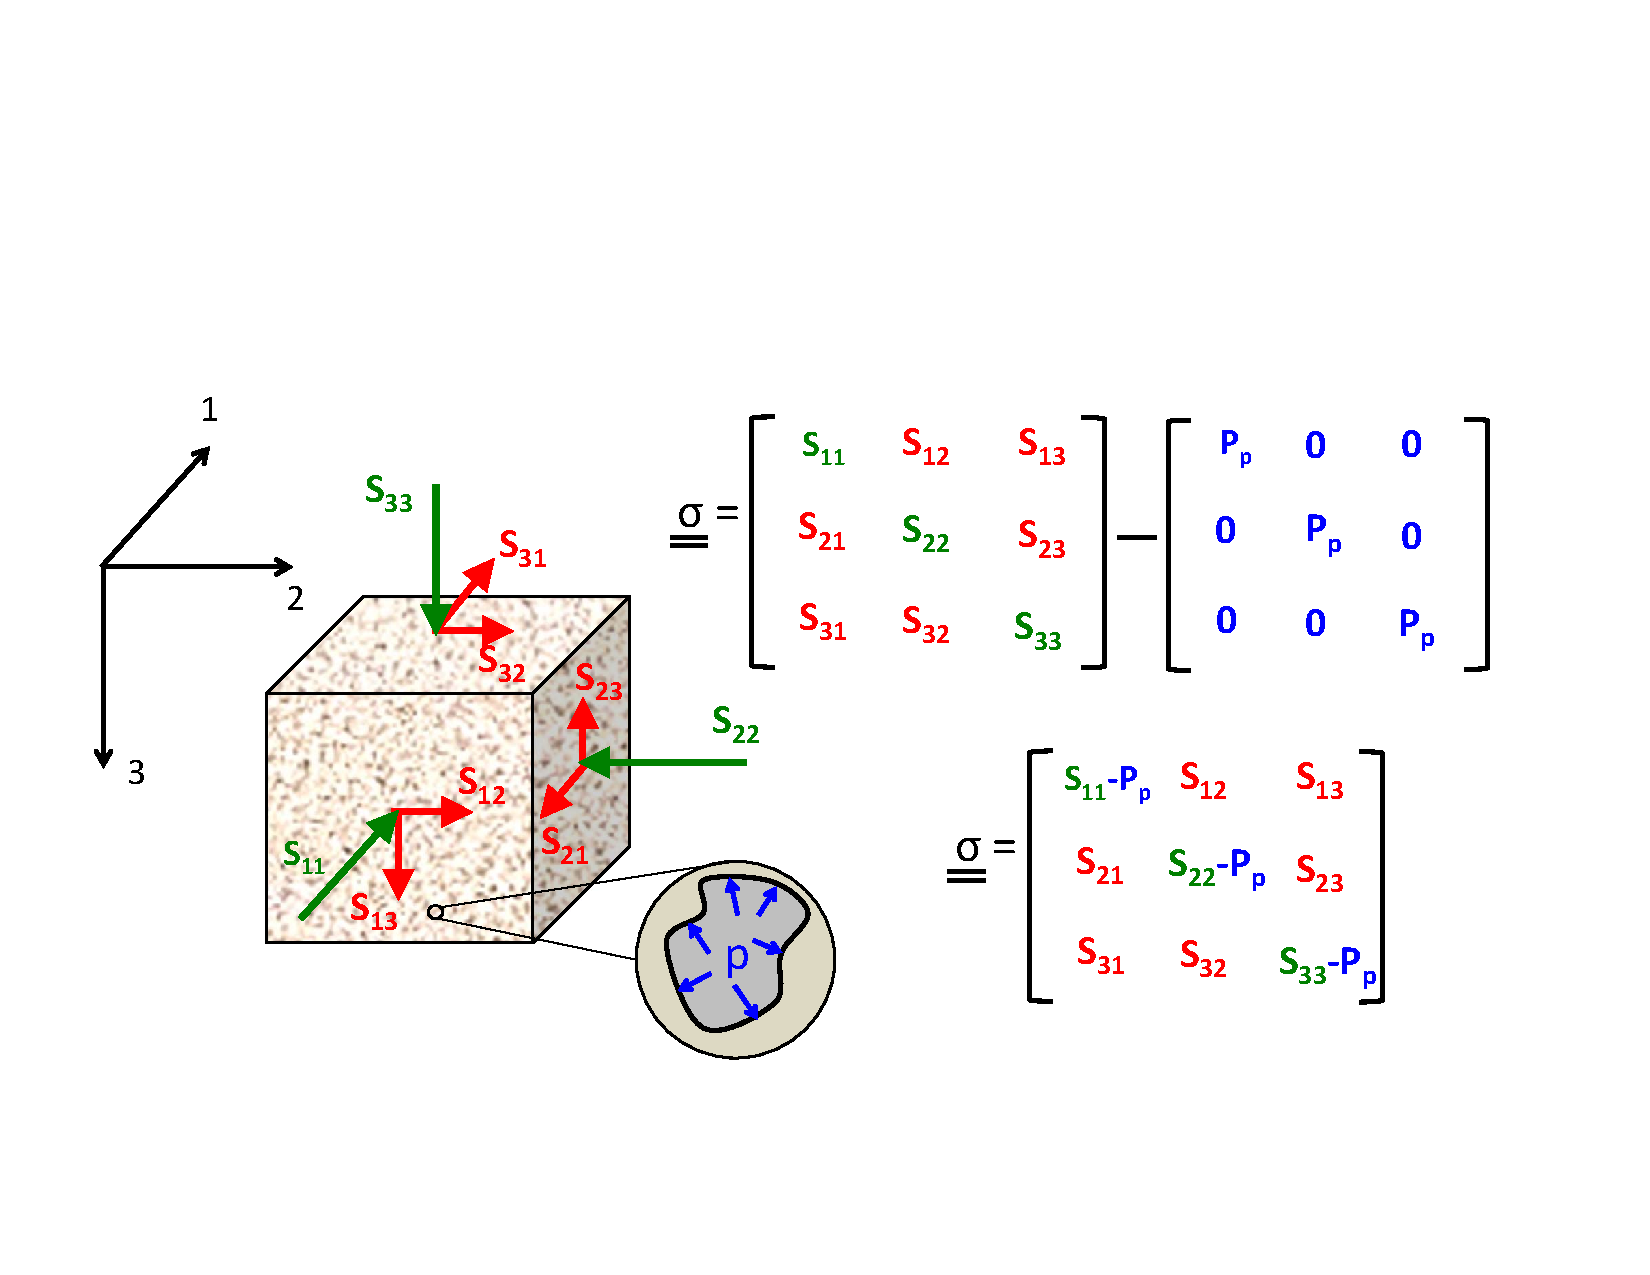
\includegraphics[scale=0.55]{.././Figures/split/4-26.pdf}%
\lthtmlpictureZ
\lthtmlcheckvsize\clearpage}

{\newpage\clearpage
\lthtmlinlinemathA{tex2html_wrap_indisplay16179}%
$\displaystyle \uuline{\varepsilon} = \uuline{D} \: (\uuline{S} - \alpha P_p \uuline{I})$%
\lthtmlindisplaymathZ
\lthtmlcheckvsize\clearpage}

{\newpage\clearpage
\lthtmlinlinemathA{tex2html_wrap_inline16181}%
$ \alpha \sim 1$%
\lthtmlindisplaymathZ
\lthtmlcheckvsize\clearpage}

{\newpage\clearpage
\lthtmlinlinemathA{tex2html_wrap_inline16183}%
$ \alpha \sim 0.5$%
\lthtmlindisplaymathZ
\lthtmlcheckvsize\clearpage}

\stepcounter{subsection}
{\newpage\clearpage
\lthtmlinlinemathA{tex2html_wrap_inline16186}%
$ S_v = S_{33}$%
\lthtmlindisplaymathZ
\lthtmlcheckvsize\clearpage}

{\newpage\clearpage
\lthtmlinlinemathA{tex2html_wrap_indisplay16190}%
$\displaystyle \sigma_v(z) = S_v(z) - P_p$%
\lthtmlindisplaymathZ
\lthtmlcheckvsize\clearpage}

{\newpage\clearpage
\lthtmlinlinemathA{tex2html_wrap_inline16192}%
$ \varepsilon_{11}=\varepsilon_{22}$%
\lthtmlindisplaymathZ
\lthtmlcheckvsize\clearpage}

{\newpage\clearpage
\lthtmlinlinemathA{tex2html_wrap_inline16198}%
$ \uuline{\varepsilon} = [0,0,\varepsilon_{33},0,0,0]^T$%
\lthtmlindisplaymathZ
\lthtmlcheckvsize\clearpage}

{\newpage\clearpage
\lthtmlinlinemathA{tex2html_wrap_inline16200}%
$ \uuline{\sigma} = \uuline{D} \: \uuline{\varepsilon}$%
\lthtmlindisplaymathZ
\lthtmlcheckvsize\clearpage}

{\newpage\clearpage
\lthtmldisplayA{displaymath16202}%
\begin{displaymath}\left\lbrace
\begin{array}{l}
\sigma_{11} = \sigma_{22} =
\frac{\nu E}{(1+\nu)(1-2\nu)} \varepsilon_{33}  \\
\sigma_{33} = \frac{(1-\nu) E}{(1+\nu)(1-2\nu)} 		 			\varepsilon_{33}
\end{array}
\right.\end{displaymath}%
\lthtmldisplayZ
\lthtmlcheckvsize\clearpage}

{\newpage\clearpage
\lthtmlinlinemathA{tex2html_wrap_inline16208}%
$ \sigma_{11}$%
\lthtmlindisplaymathZ
\lthtmlcheckvsize\clearpage}

{\newpage\clearpage
\lthtmlinlinemathA{tex2html_wrap_inline16210}%
$ \sigma_{22}$%
\lthtmlindisplaymathZ
\lthtmlcheckvsize\clearpage}

{\newpage\clearpage
\lthtmlinlinemathA{tex2html_wrap_indisplay16212}%
$\displaystyle \sigma_{11} = \sigma_{22} = \frac{\nu}{1-\nu} \sigma_{33}$%
\lthtmlindisplaymathZ
\lthtmlcheckvsize\clearpage}

{\newpage\clearpage
\lthtmlinlinemathA{tex2html_wrap_indisplay16214}%
$\displaystyle \sigma_{h} = \frac{\nu}{1-\nu} \sigma_{v}$%
\lthtmlindisplaymathZ
\lthtmlcheckvsize\clearpage}

{\newpage\clearpage
\lthtmlinlinemathA{tex2html_wrap_inline16216}%
$ \nu \sim 0.25$%
\lthtmlindisplaymathZ
\lthtmlcheckvsize\clearpage}

{\newpage\clearpage
\lthtmlinlinemathA{tex2html_wrap_inline16218}%
$ \nu/(1-\nu) \sim 1/3 $%
\lthtmlindisplaymathZ
\lthtmlcheckvsize\clearpage}

{\newpage\clearpage
\lthtmlinlinemathA{tex2html_wrap_inline16220}%
$ \nu \rightarrow 0.5$%
\lthtmlindisplaymathZ
\lthtmlcheckvsize\clearpage}

{\newpage\clearpage
\lthtmlinlinemathA{tex2html_wrap_inline16222}%
$ \nu/(1-\nu) \rightarrow 1$%
\lthtmlindisplaymathZ
\lthtmlcheckvsize\clearpage}

{\newpage\clearpage
\lthtmlinlinemathA{tex2html_wrap_inline16224}%
$ \nu \sim 0.5$%
\lthtmlindisplaymathZ
\lthtmlcheckvsize\clearpage}

{\newpage\clearpage
\lthtmlinlinemathA{tex2html_wrap_inline16230}%
$ S_{11} = \sigma_{11} + P_p$%
\lthtmlindisplaymathZ
\lthtmlcheckvsize\clearpage}

{\newpage\clearpage
\lthtmlinlinemathA{tex2html_wrap_inline16232}%
$ S_{33} = \sigma_{33} + P_p$%
\lthtmlindisplaymathZ
\lthtmlcheckvsize\clearpage}

{\newpage\clearpage
\lthtmlinlinemathA{tex2html_wrap_inline16234}%
$ \varepsilon_{11} \neq \varepsilon_{22} \neq 0$%
\lthtmlindisplaymathZ
\lthtmlcheckvsize\clearpage}

{\newpage\clearpage
\lthtmlinlinemathA{tex2html_wrap_inline16236}%
$ \uuline{\sigma} = \uuline{C} \: \uuline{\varepsilon}$%
\lthtmlindisplaymathZ
\lthtmlcheckvsize\clearpage}

{\newpage\clearpage
\lthtmlinlinemathA{tex2html_wrap_inline16238}%
$ \uuline{\varepsilon} = [\varepsilon_{11},\varepsilon_{22},\varepsilon_{33},0,0,0]^T$%
\lthtmlindisplaymathZ
\lthtmlcheckvsize\clearpage}

{\newpage\clearpage
\lthtmldisplayA{displaymath16240}%
\begin{displaymath}\left\lbrace
\begin{array}{l}
\sigma_{11} =
\cfrac{(1-\nu) E}{(1+\nu)(1-2\nu)} \varepsilon_{11}
+ \cfrac{\nu E}{(1+\nu)(1-2\nu)} \varepsilon_{22}
+ \cfrac{\nu E}{(1+\nu)(1-2\nu)} \varepsilon_{33} \\
\sigma_{22} =
\cfrac{\nu E}{(1+\nu)(1-2\nu)} \varepsilon_{11}
+ \cfrac{(1-\nu) E}{(1+\nu)(1-2\nu)} \varepsilon_{22}
+ \cfrac{\nu E}{(1+\nu)(1-2\nu)} \varepsilon_{33} \\
\sigma_{33} =
\cfrac{\nu E}{(1+\nu)(1-2\nu)} \varepsilon_{11}
+   \cfrac{\nu E}{(1+\nu)(1-2\nu)} \varepsilon_{22}
+	\cfrac{(1-\nu) E}{(1+\nu)(1-2\nu)} \varepsilon_{33}
\end{array}
\right.\end{displaymath}%
\lthtmldisplayZ
\lthtmlcheckvsize\clearpage}

{\newpage\clearpage
\lthtmldisplayA{displaymath16250}%
\begin{displaymath}\left\lbrace
\begin{array}{l}
\sigma_{11} =
\cfrac{\nu}{1-\nu} \sigma_{33} +
\cfrac{E}{1-\nu^2} \varepsilon_{11} +
\cfrac{\nu E}{1-\nu^2} \varepsilon_{22} \\
\sigma_{22} =
\cfrac{\nu}{1-\nu} \sigma_{33} +
\cfrac{\nu E}{1-\nu^2} \varepsilon_{11} +
\cfrac{E}{1-\nu^2} \varepsilon_{22} \\
\end{array}
\right.\end{displaymath}%
\lthtmldisplayZ
\lthtmlcheckvsize\clearpage}

{\newpage\clearpage
\lthtmlinlinemathA{tex2html_wrap_inline16252}%
$ \varepsilon_{Hmax}$%
\lthtmlindisplaymathZ
\lthtmlcheckvsize\clearpage}

{\newpage\clearpage
\lthtmlinlinemathA{tex2html_wrap_inline16254}%
$ \varepsilon_{hmin}$%
\lthtmlindisplaymathZ
\lthtmlcheckvsize\clearpage}

{\newpage\clearpage
\lthtmldisplayA{displaymath16256}%
\begin{displaymath}\left\lbrace
\begin{array}{l}
\sigma_{Hmax} =  \cfrac{\nu}{1-\nu} \sigma_{v} +
E' \varepsilon_{Hmax} +
\nu E'\varepsilon_{hmin}  \\
\sigma_{hmin} =  \cfrac{\nu}{1-\nu} \sigma_{v} +
\nu E' \varepsilon_{Hmax} +
E' \varepsilon_{hmin} \\
\end{array}
\right.\end{displaymath}%
\lthtmldisplayZ
\lthtmlcheckvsize\clearpage}

{\newpage\clearpage
\lthtmlinlinemathA{tex2html_wrap_inline16258}%
$ E' = \frac{E}{1-\nu^2}$%
\lthtmlindisplaymathZ
\lthtmlcheckvsize\clearpage}

{\newpage\clearpage
\lthtmlinlinemathA{tex2html_wrap_inline16260}%
$ S_{Hmax} = \sigma_{Hmax} + P_p$%
\lthtmlindisplaymathZ
\lthtmlcheckvsize\clearpage}

{\newpage\clearpage
\lthtmlinlinemathA{tex2html_wrap_inline16262}%
$ S_{hmin} = \sigma_{hmin} + P_p$%
\lthtmlindisplaymathZ
\lthtmlcheckvsize\clearpage}

{\newpage\clearpage
\lthtmlinlinemathA{tex2html_wrap_inline16264}%
$ \sigma_{v} = S_{v} - P_p$%
\lthtmlindisplaymathZ
\lthtmlcheckvsize\clearpage}

{\newpage\clearpage
\lthtmlinlinemathA{tex2html_wrap_inline16270}%
$ K$%
\lthtmlindisplaymathZ
\lthtmlcheckvsize\clearpage}

{\newpage\clearpage
\lthtmlinlinemathA{tex2html_wrap_inline16272}%
$ G$%
\lthtmlindisplaymathZ
\lthtmlcheckvsize\clearpage}

{\newpage\clearpage
\lthtmlpictureA{tex2html_wrap16274}%
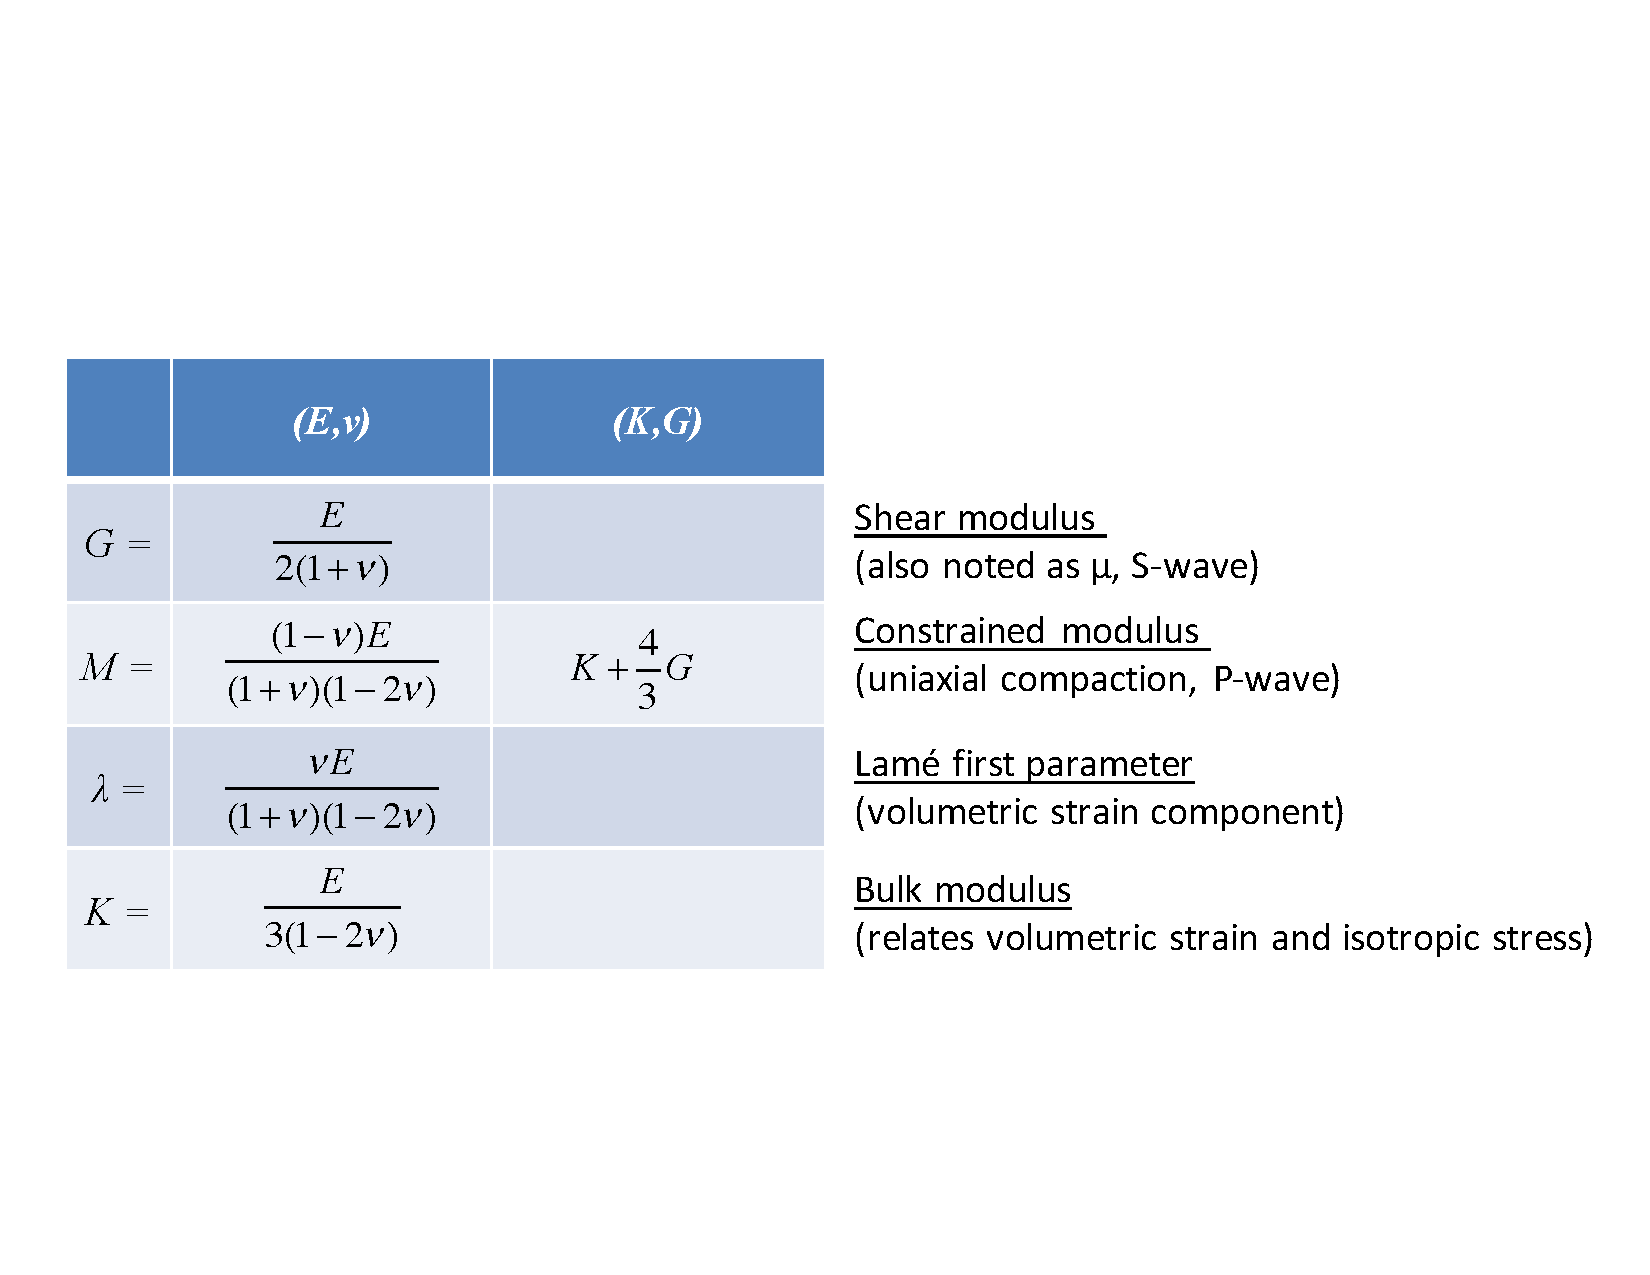
\includegraphics[scale=0.55]{.././Figures/split/4-21.pdf}%
\lthtmlpictureZ
\lthtmlcheckvsize\clearpage}

{\newpage\clearpage
\lthtmlinlinemathA{tex2html_wrap_inline16279}%
$ \mathrm{d}S_v/\mathrm{d}z = 23.8$%
\lthtmlindisplaymathZ
\lthtmlcheckvsize\clearpage}

{\newpage\clearpage
\lthtmlinlinemathA{tex2html_wrap_inline16281}%
$ \lambda_p = 0.7$%
\lthtmlindisplaymathZ
\lthtmlcheckvsize\clearpage}

{\newpage\clearpage
\lthtmlinlinemathA{tex2html_wrap_inline16283}%
$ E = 5$%
\lthtmlindisplaymathZ
\lthtmlcheckvsize\clearpage}

{\newpage\clearpage
\lthtmlinlinemathA{tex2html_wrap_inline16285}%
$ \nu = 0.22$%
\lthtmlindisplaymathZ
\lthtmlcheckvsize\clearpage}

{\newpage\clearpage
\lthtmlinlinemathA{tex2html_wrap_inline16287}%
$ \varepsilon_{hmin} = 0$%
\lthtmlindisplaymathZ
\lthtmlcheckvsize\clearpage}

{\newpage\clearpage
\lthtmlinlinemathA{tex2html_wrap_inline16289}%
$ \varepsilon_{Hmax} = 0.0002$%
\lthtmlindisplaymathZ
\lthtmlcheckvsize\clearpage}

{\newpage\clearpage
\lthtmlinlinemathA{tex2html_wrap_indisplay16291}%
$\displaystyle S_v = 23.8 \frac{\text{MPa}}{\text{km}} \times \frac{1\frac{\text{psi}}{\text{ft}}}{\frac{\text{MPa}}{\text{km}}} \times 7950 \text{ ft} = 8227 \text {psi}
$%
\lthtmlindisplaymathZ
\lthtmlcheckvsize\clearpage}

{\newpage\clearpage
\lthtmlinlinemathA{tex2html_wrap_indisplay16293}%
$\displaystyle P_p = \lambda_p S_v = 0.7 \times 8227$%
\lthtmlindisplaymathZ
\lthtmlcheckvsize\clearpage}

{\newpage\clearpage
\lthtmlinlinemathA{tex2html_wrap_indisplay16294}%
$\displaystyle \text {psi} = 5759 \text{ psi}
$%
\lthtmlindisplaymathZ
\lthtmlcheckvsize\clearpage}

{\newpage\clearpage
\lthtmlinlinemathA{tex2html_wrap_indisplay16296}%
$\displaystyle \sigma_v = S_v - P_p = 8227$%
\lthtmlindisplaymathZ
\lthtmlcheckvsize\clearpage}

{\newpage\clearpage
\lthtmlinlinemathA{tex2html_wrap_indisplay16297}%
$\displaystyle \text {psi} - 5759 \text{ psi} = 2468 \text{ psi}
$%
\lthtmlindisplaymathZ
\lthtmlcheckvsize\clearpage}

{\newpage\clearpage
\lthtmlinlinemathA{tex2html_wrap_indisplay16299}%
$\displaystyle E' = \frac{E}{1-\nu^2} = \frac{5 \times 10^6 \text{ psi}}{1-0.22^2} = 5.25 \times 10^6 \text{ psi}
$%
\lthtmlindisplaymathZ
\lthtmlcheckvsize\clearpage}

{\newpage\clearpage
\lthtmldisplayA{displaymath16301}%
\begin{displaymath}\left\lbrace
\begin{array}{l}
\sigma_{Hmax} =  \frac{\nu}{1-\nu} \sigma_{v} +
E' \varepsilon_{Hmax} +
\nu E'\varepsilon_{hmin} =
\frac{0.22}{1-0.22} 2468 \text{ psi} +
5.25 \times 10^6 \text{ psi} \times 0.0002 = 1745 \text{ psi}\\
\sigma_{hmin} =  \frac{\nu}{1-\nu} \sigma_{v} +
\nu E' \varepsilon_{Hmax} +
E' \varepsilon_{hmin} =
\frac{0.22}{1-0.22} 2468 \text{ psi} +
0.22 \times 5.25 \times 10^6 \text{ psi} \times 0.0002 = 927 \text{ psi}  \\
\end{array}
\right.\end{displaymath}%
\lthtmldisplayZ
\lthtmlcheckvsize\clearpage}

{\newpage\clearpage
\lthtmldisplayA{displaymath16303}%
\begin{displaymath}\left\lbrace
\begin{array}{l}
S_{Hmax} = \sigma_{Hmax} + P_p =  1745 \text{ psi} + 5759 \text{ psi} = 7504 \text{ psi}\\
S_{hmin} = \sigma_{hmin} + P_p =  927 \text{ psi} + 5759 \text{ psi} = 6686 \text{ psi}
\end{array}
\right. \: \: \blacksquare\end{displaymath}%
\lthtmldisplayZ
\lthtmlcheckvsize\clearpage}

\stepcounter{subsection}
{\newpage\clearpage
\lthtmlinlinemathA{tex2html_wrap_inline16306}%
$ C_{pp}$%
\lthtmlindisplaymathZ
\lthtmlcheckvsize\clearpage}

{\newpage\clearpage
\lthtmlinlinemathA{tex2html_wrap_inline16308}%
$ V_p$%
\lthtmlindisplaymathZ
\lthtmlcheckvsize\clearpage}

{\newpage\clearpage
\lthtmlinlinemathA{tex2html_wrap_indisplay16310}%
$\displaystyle C_{pp} = \left. \frac{1}{V_p} \frac{\mathrm{d}V_p}{\mathrm{d}P_p} \right|_{S_v,\varepsilon_h}$%
\lthtmlindisplaymathZ
\lthtmlcheckvsize\clearpage}

{\newpage\clearpage
\lthtmlinlinemathA{tex2html_wrap_inline16314}%
$ \varepsilon_h$%
\lthtmlindisplaymathZ
\lthtmlcheckvsize\clearpage}

{\newpage\clearpage
\lthtmlinlinemathA{tex2html_wrap_indisplay16320}%
$\displaystyle C_{pp} = \frac{C_{bp}}{\phi}$%
\lthtmlindisplaymathZ
\lthtmlcheckvsize\clearpage}

{\newpage\clearpage
\lthtmlinlinemathA{tex2html_wrap_inline16322}%
$ C_{bp} \sim 1/M$%
\lthtmlindisplaymathZ
\lthtmlcheckvsize\clearpage}

{\newpage\clearpage
\lthtmlinlinemathA{tex2html_wrap_inline16324}%
$ M = (1-\nu) E / [(1+\nu)(1-2\nu)]$%
\lthtmlindisplaymathZ
\lthtmlcheckvsize\clearpage}

{\newpage\clearpage
\lthtmlinlinemathA{tex2html_wrap_indisplay16330}%
$\displaystyle C_{pp} = \frac{(1+\nu)(1-2\nu)}{(1-\nu) E \phi}$%
\lthtmlindisplaymathZ
\lthtmlcheckvsize\clearpage}

{\newpage\clearpage
\lthtmlinlinemathA{tex2html_wrap_inline16342}%
$ E = 10$%
\lthtmlindisplaymathZ
\lthtmlcheckvsize\clearpage}

{\newpage\clearpage
\lthtmlinlinemathA{tex2html_wrap_inline16344}%
$ \nu = 0.20$%
\lthtmlindisplaymathZ
\lthtmlcheckvsize\clearpage}

{\newpage\clearpage
\lthtmlinlinemathA{tex2html_wrap_inline16346}%
$ 10^{6}$%
\lthtmlindisplaymathZ
\lthtmlcheckvsize\clearpage}

{\newpage\clearpage
\lthtmlinlinemathA{tex2html_wrap_indisplay16350}%
$\displaystyle M = \frac{(1-\nu) E}{(1+\nu)(1-2\nu)} = \frac{(1-0.20) 10 \text{ GPa} }{(1+0.20)(1-2 \times 0.20)} = 11.11 \text{ GPa} = 1.6 \times 10^{6} \text{ psi}
$%
\lthtmlindisplaymathZ
\lthtmlcheckvsize\clearpage}

{\newpage\clearpage
\lthtmlinlinemathA{tex2html_wrap_indisplay16352}%
$\displaystyle C_{pp} = \frac{1}{M \phi} = \frac{1}{1.6 \times 10^{6} psi \times 0.20} = 3.1 \: [10^{6}$%
\lthtmlindisplaymathZ
\lthtmlcheckvsize\clearpage}

{\newpage\clearpage
\lthtmlinlinemathA{tex2html_wrap_indisplay16353}%
$\displaystyle ]^{-1} = 3.1 \: \mu$%
\lthtmlindisplaymathZ
\lthtmlcheckvsize\clearpage}

{\newpage\clearpage
\lthtmlinlinemathA{tex2html_wrap_indisplay16354}%
$\displaystyle \: \: \blacksquare
$%
\lthtmlindisplaymathZ
\lthtmlcheckvsize\clearpage}

\stepcounter{subsection}
{\newpage\clearpage
\lthtmlinlinemathA{tex2html_wrap_inline16357}%
$ \uline{u}$%
\lthtmlindisplaymathZ
\lthtmlcheckvsize\clearpage}

{\newpage\clearpage
\lthtmlinlinemathA{tex2html_wrap_indisplay16359}%
$\displaystyle (\lambda + G) \nabla (\nabla \cdot \uline{u}) +
G \nabla^2 \uline{u} + \rho \uline{b} = 0$%
\lthtmlindisplaymathZ
\lthtmlcheckvsize\clearpage}

{\newpage\clearpage
\lthtmlinlinemathA{tex2html_wrap_inline16361}%
$ \lambda = (\nu E)/[(1+\nu)(1-2\nu)]$%
\lthtmlindisplaymathZ
\lthtmlcheckvsize\clearpage}

{\newpage\clearpage
\lthtmlinlinemathA{tex2html_wrap_inline16369}%
$ \nabla ()$%
\lthtmlindisplaymathZ
\lthtmlcheckvsize\clearpage}

{\newpage\clearpage
\lthtmlinlinemathA{tex2html_wrap_inline16371}%
$ \nabla \cdot ()$%
\lthtmlindisplaymathZ
\lthtmlcheckvsize\clearpage}

{\newpage\clearpage
\lthtmlinlinemathA{tex2html_wrap_inline16373}%
$ \nabla^2 ()$%
\lthtmlindisplaymathZ
\lthtmlcheckvsize\clearpage}

\stepcounter{section}
{\newpage\clearpage
\lthtmlpictureA{tex2html_wrap16376}%
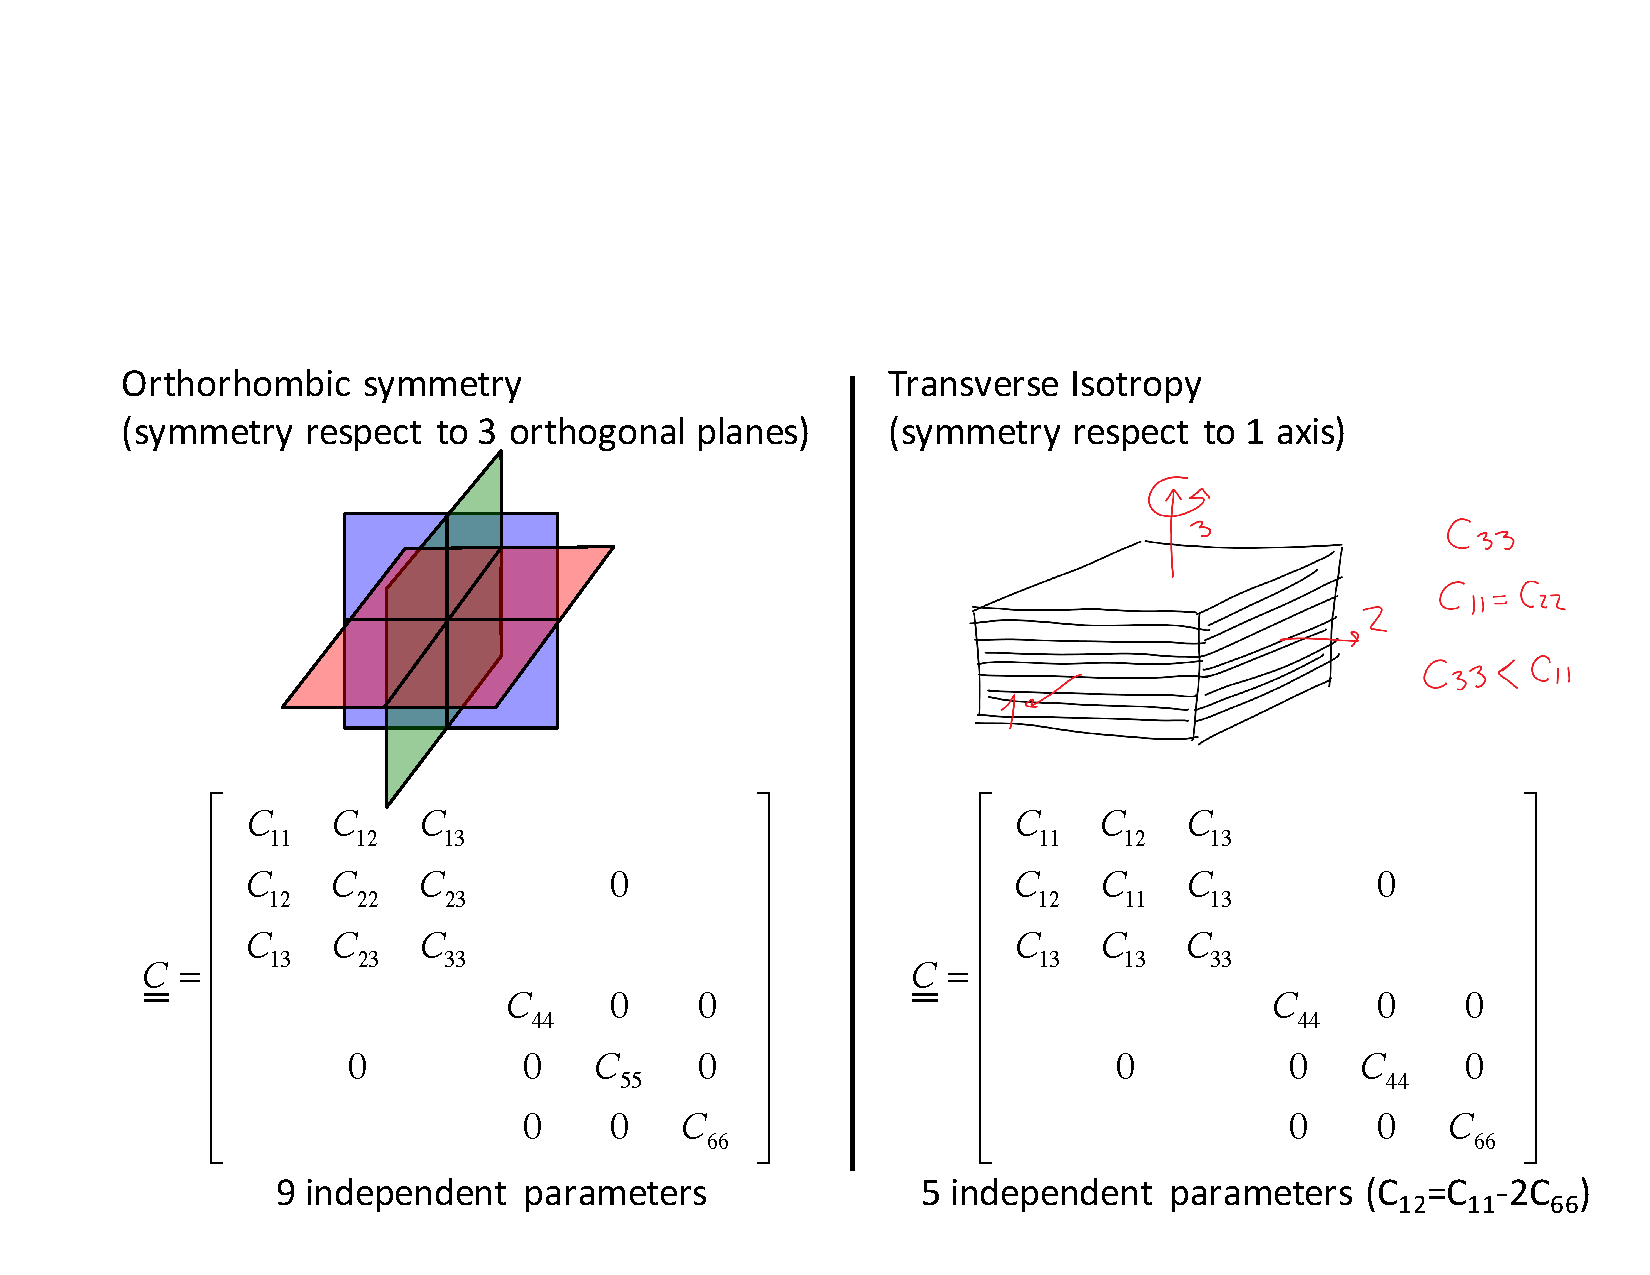
\includegraphics[scale=0.55]{.././Figures/split/4-22.pdf}%
\lthtmlpictureZ
\lthtmlcheckvsize\clearpage}

{\newpage\clearpage
\lthtmlinlinemathA{tex2html_wrap_inline16381}%
$ E_h > E_v$%
\lthtmlindisplaymathZ
\lthtmlcheckvsize\clearpage}

\stepcounter{section}
{\newpage\clearpage
\lthtmlinlinemathA{tex2html_wrap_inline16388}%
$ \varepsilon \gtrsim 0.001$%
\lthtmlindisplaymathZ
\lthtmlcheckvsize\clearpage}

{\newpage\clearpage
\lthtmlinlinemathA{tex2html_wrap_inline16390}%
$ E_{load}$%
\lthtmlindisplaymathZ
\lthtmlcheckvsize\clearpage}

{\newpage\clearpage
\lthtmlinlinemathA{tex2html_wrap_inline16392}%
$ E_{unload}$%
\lthtmlindisplaymathZ
\lthtmlcheckvsize\clearpage}

{\newpage\clearpage
\lthtmlinlinemathA{tex2html_wrap_inline16398}%
$ E_{unload} \sim E_{unload}$%
\lthtmlindisplaymathZ
\lthtmlcheckvsize\clearpage}

{\newpage\clearpage
\lthtmlpictureA{tex2html_wrap16400}%
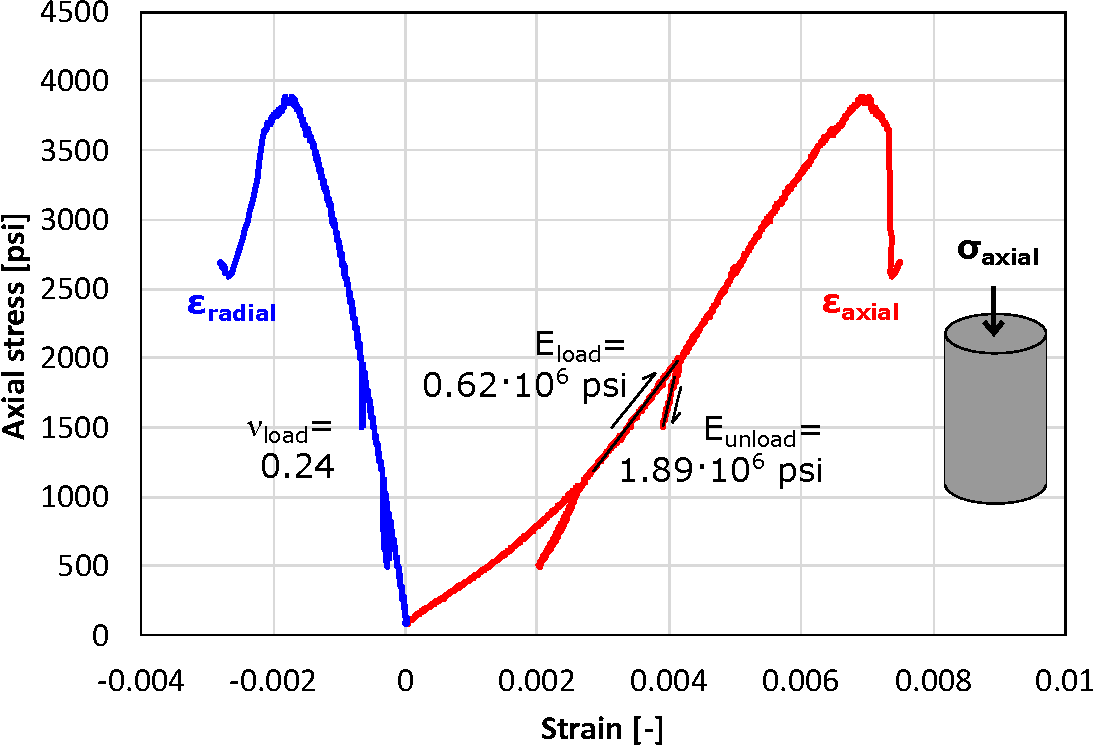
\includegraphics[scale=0.55]{.././Figures/split/LoadingUnloading.pdf}%
\lthtmlpictureZ
\lthtmlcheckvsize\clearpage}

\stepcounter{section}
{\newpage\clearpage
\lthtmlpictureA{tex2html_wrap16410}%
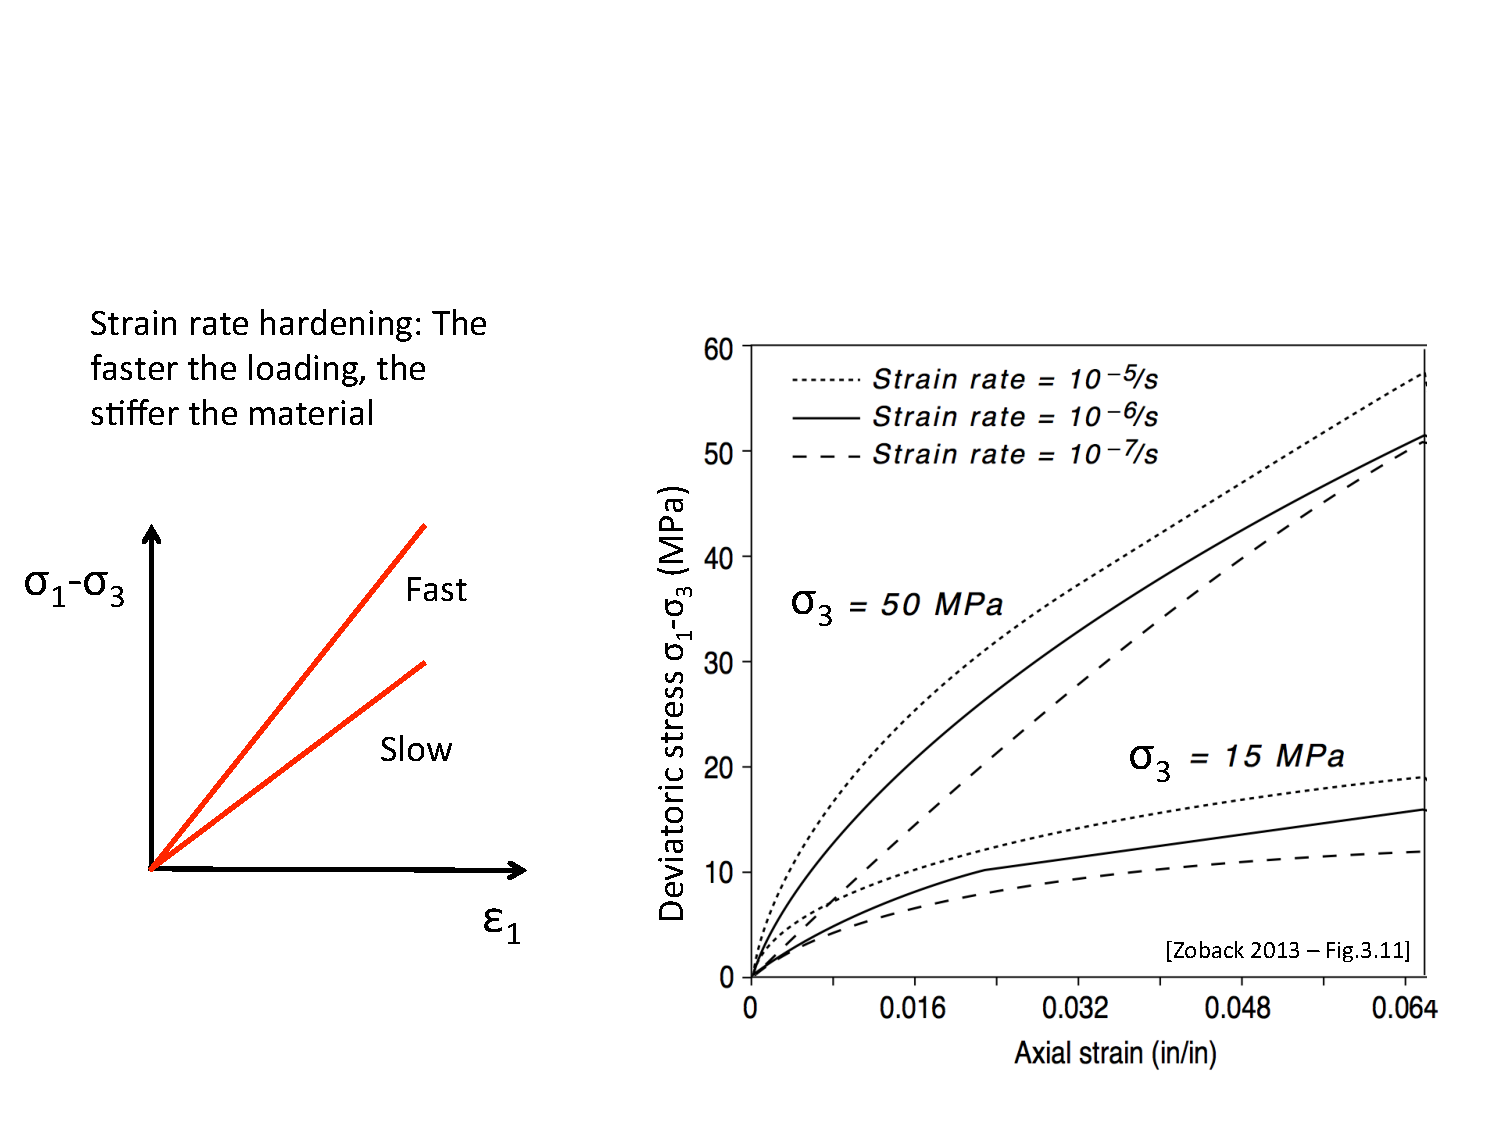
\includegraphics[scale=0.50]{.././Figures/split/5B-18.pdf}%
\lthtmlpictureZ
\lthtmlcheckvsize\clearpage}

{\newpage\clearpage
\lthtmlpictureA{tex2html_wrap16415}%
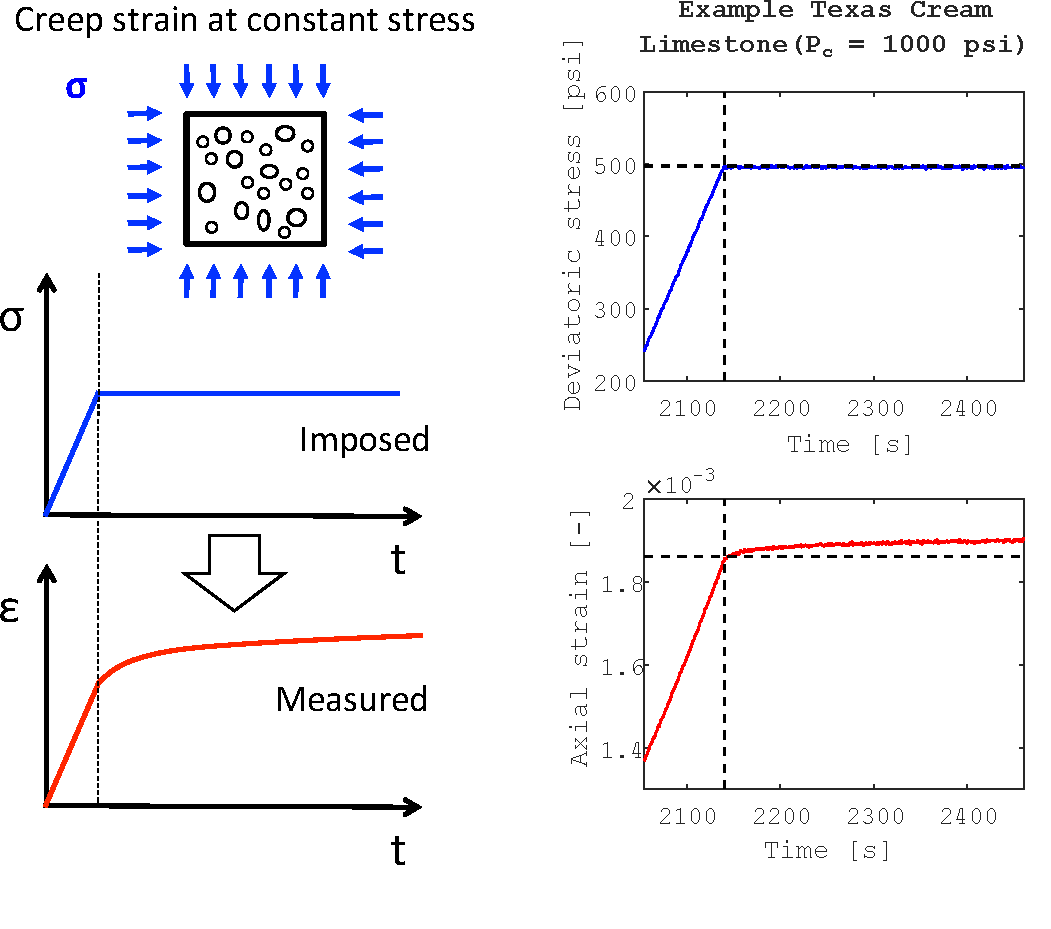
\includegraphics[scale=0.60]{.././Figures/split/5-CreepTXC.pdf}%
\lthtmlpictureZ
\lthtmlcheckvsize\clearpage}

{\newpage\clearpage
\lthtmlpictureA{tex2html_wrap16420}%
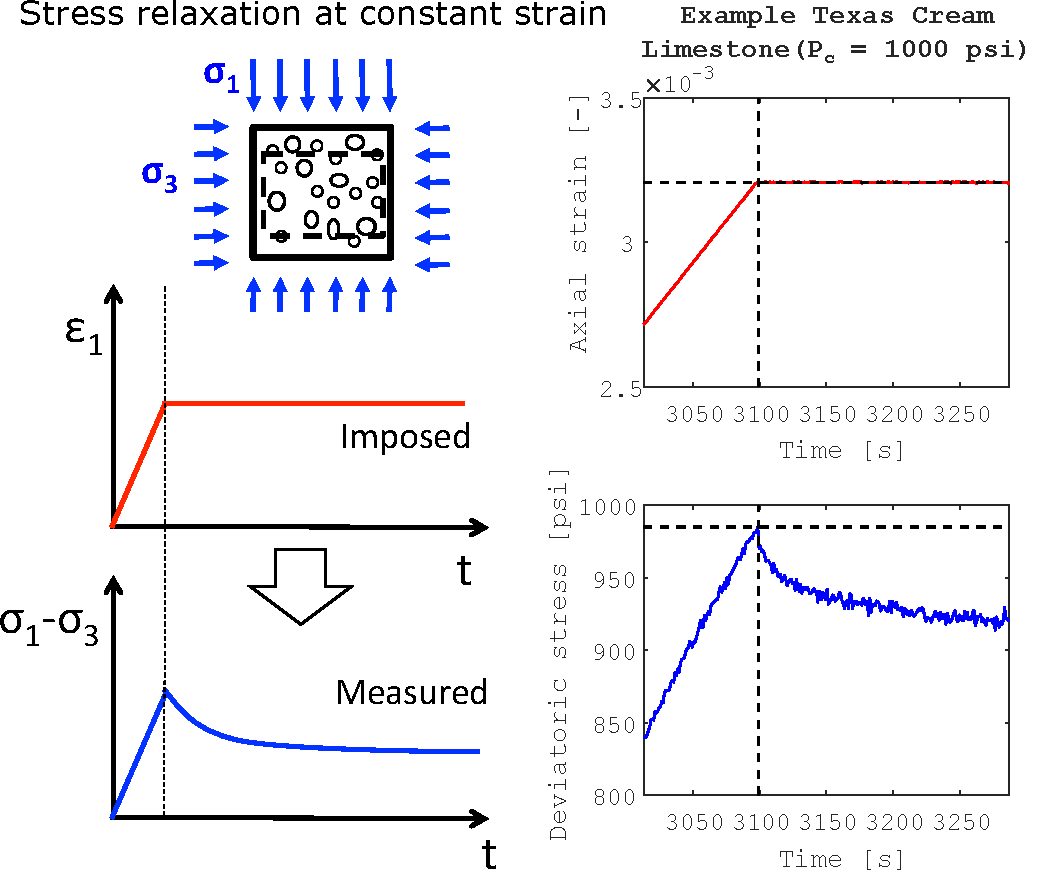
\includegraphics[scale=0.60]{.././Figures/split/5-StressRelaxTXC.pdf}%
\lthtmlpictureZ
\lthtmlcheckvsize\clearpage}

\stepcounter{section}
\stepcounter{subsection}
{\newpage\clearpage
\lthtmlinlinemathA{tex2html_wrap_inline16427}%
$ \uuline{\varepsilon} = \uuline{D} \: \uuline{\sigma}$%
\lthtmlindisplaymathZ
\lthtmlcheckvsize\clearpage}

{\newpage\clearpage
\lthtmlinlinemathA{tex2html_wrap_indisplay16429}%
$\displaystyle \uuline{\sigma} = \uuline{S} - \alpha P_p \uuline{I}$%
\lthtmlindisplaymathZ
\lthtmlcheckvsize\clearpage}

{\newpage\clearpage
\lthtmlinlinemathA{tex2html_wrap_inline16433}%
$ \uuline{I}$%
\lthtmlindisplaymathZ
\lthtmlcheckvsize\clearpage}

{\newpage\clearpage
\lthtmlinlinemathA{tex2html_wrap_indisplay16435}%
$\displaystyle \alpha = 1 - \frac{K_{drained}}{K_{unj}}$%
\lthtmlindisplaymathZ
\lthtmlcheckvsize\clearpage}

{\newpage\clearpage
\lthtmlinlinemathA{tex2html_wrap_inline16437}%
$ K_{drained}$%
\lthtmlindisplaymathZ
\lthtmlcheckvsize\clearpage}

{\newpage\clearpage
\lthtmlinlinemathA{tex2html_wrap_inline16439}%
$ K_{unj}$%
\lthtmlindisplaymathZ
\lthtmlcheckvsize\clearpage}

{\newpage\clearpage
\lthtmlinlinemathA{tex2html_wrap_inline16441}%
$ K_{unj} = K_{m}$%
\lthtmlindisplaymathZ
\lthtmlcheckvsize\clearpage}

{\newpage\clearpage
\lthtmlinlinemathA{tex2html_wrap_inline16443}%
$ \uuline{\alpha}$%
\lthtmlindisplaymathZ
\lthtmlcheckvsize\clearpage}

{\newpage\clearpage
\lthtmlinlinemathA{tex2html_wrap_inline16445}%
$ \alpha \neq 1$%
\lthtmlindisplaymathZ
\lthtmlcheckvsize\clearpage}

\stepcounter{subsection}
{\newpage\clearpage
\lthtmlpictureA{tex2html_wrap16448}%
\includegraphics[scale=0.55]{.././Figures/split/4-23.pdf}%
\lthtmlpictureZ
\lthtmlcheckvsize\clearpage}

{\newpage\clearpage
\lthtmlinlinemathA{tex2html_wrap_inline16453}%
$ \alpha_L$%
\lthtmlindisplaymathZ
\lthtmlcheckvsize\clearpage}

{\newpage\clearpage
\lthtmlinlinemathA{tex2html_wrap_inline16457}%
$ p$%
\lthtmlindisplaymathZ
\lthtmlcheckvsize\clearpage}

{\newpage\clearpage
\lthtmlinlinemathA{tex2html_wrap_indisplay16459}%
$\displaystyle \alpha_L = \left. \cfrac{1}{L} \cfrac{ \mathrm{d} L}{ \mathrm{d} T} \right|_p$%
\lthtmlindisplaymathZ
\lthtmlcheckvsize\clearpage}

{\newpage\clearpage
\lthtmlinlinemathA{tex2html_wrap_inline16461}%
$ \Delta T$%
\lthtmlindisplaymathZ
\lthtmlcheckvsize\clearpage}

{\newpage\clearpage
\lthtmldisplayA{displaymath16463}%
\begin{displaymath}\left\lbrace
\begin{array}{rcl}
\sigma_{11} & = & (\lambda + 2 \mu) \: \varepsilon_{11} + \lambda \: \varepsilon_{22} + \lambda \: \varepsilon_{33} + 3 K \alpha_L \Delta T \\
\sigma_{22} & = & \lambda \: \varepsilon_{11} + (\lambda + 2 \mu) \: \varepsilon_{22} + \lambda \: \varepsilon_{33} + 3 K \alpha_L \Delta T \\
\sigma_{33} & = & \lambda \: \varepsilon_{11} + \lambda \: \varepsilon_{22} + (\lambda + 2 \mu) \: \varepsilon_{33} + 3 K \alpha_L \Delta T \\
\sigma_{12} & = & 2 \mu \: \varepsilon_{12}\\
\sigma_{13} & = & 2 \mu \: \varepsilon_{13}\\
\sigma_{23} & = & 2 \mu \: \varepsilon_{23}\\
\end{array}
\right.\end{displaymath}%
\lthtmldisplayZ
\lthtmlcheckvsize\clearpage}

{\newpage\clearpage
\lthtmlinlinemathA{tex2html_wrap_inline16465}%
$ \sigma_{11}=\sigma_{22}=0$%
\lthtmlindisplaymathZ
\lthtmlcheckvsize\clearpage}

{\newpage\clearpage
\lthtmlinlinemathA{tex2html_wrap_inline16467}%
$ \varepsilon_{11}=\varepsilon_{22} \neq 0$%
\lthtmlindisplaymathZ
\lthtmlcheckvsize\clearpage}

{\newpage\clearpage
\lthtmlinlinemathA{tex2html_wrap_inline16469}%
$ \varepsilon_{33}=0$%
\lthtmlindisplaymathZ
\lthtmlcheckvsize\clearpage}

{\newpage\clearpage
\lthtmlinlinemathA{tex2html_wrap_inline16471}%
$ \Delta T \neq 0$%
\lthtmlindisplaymathZ
\lthtmlcheckvsize\clearpage}

{\newpage\clearpage
\lthtmldisplayA{displaymath16473}%
\begin{displaymath}\left\lbrace
\begin{array}{rcl}
0 & = & (\lambda + 2 \mu) \: \varepsilon_{11} + \lambda \: \varepsilon_{11} + 3 K \alpha_L \Delta T\\
\sigma_{33} & = & \lambda \: \varepsilon_{11} + \lambda \: \varepsilon_{11} + 3 K \alpha_L \Delta T \\
\end{array}
\right.\end{displaymath}%
\lthtmldisplayZ
\lthtmlcheckvsize\clearpage}

{\newpage\clearpage
\lthtmlinlinemathA{tex2html_wrap_indisplay16479}%
$\displaystyle \sigma_{33} = \left( \frac{6-\mu/K}{3+\mu/K} \right) K \alpha_L \Delta T \: \: \blacksquare
$%
\lthtmlindisplaymathZ
\lthtmlcheckvsize\clearpage}

\stepcounter{section}
{\newpage\clearpage
\lthtmlinlinemathA{tex2html_wrap_inline16482}%
$ D = 1.00$%
\lthtmlindisplaymathZ
\lthtmlcheckvsize\clearpage}

{\newpage\clearpage
\lthtmlinlinemathA{tex2html_wrap_inline16484}%
$ L = 2.01$%
\lthtmlindisplaymathZ
\lthtmlcheckvsize\clearpage}

{\newpage\clearpage
\lthtmlinlinemathA{tex2html_wrap_inline16486}%
$ \Delta L$%
\lthtmlindisplaymathZ
\lthtmlcheckvsize\clearpage}

{\newpage\clearpage
\lthtmlinlinemathA{tex2html_wrap_inline16488}%
$ \Delta D$%
\lthtmlindisplaymathZ
\lthtmlcheckvsize\clearpage}

{\newpage\clearpage
\lthtmlinlinemathA{tex2html_wrap_inline16491}%
$ \uline{\sigma} = \uuline{C} \: \uline{\varepsilon}$%
\lthtmlindisplaymathZ
\lthtmlcheckvsize\clearpage}

{\newpage\clearpage
\lthtmlinlinemathA{tex2html_wrap_inline16493}%
$ \sigma_{iso}$%
\lthtmlindisplaymathZ
\lthtmlcheckvsize\clearpage}

{\newpage\clearpage
\lthtmlinlinemathA{tex2html_wrap_inline16495}%
$ \varepsilon_{vol}=\frac{3(1-2\nu)}{E} \sigma_{iso}$%
\lthtmlindisplaymathZ
\lthtmlcheckvsize\clearpage}

{\newpage\clearpage
\lthtmlinlinemathA{tex2html_wrap_inline16497}%
$ \varepsilon_{vol}$%
\lthtmlindisplaymathZ
\lthtmlcheckvsize\clearpage}

{\newpage\clearpage
\lthtmlinlinemathA{tex2html_wrap_inline16499}%
$ E = 4$%
\lthtmlindisplaymathZ
\lthtmlcheckvsize\clearpage}

{\newpage\clearpage
\lthtmlinlinemathA{tex2html_wrap_inline16501}%
$ \nu = 0.2$%
\lthtmlindisplaymathZ
\lthtmlcheckvsize\clearpage}

{\newpage\clearpage
\lthtmlinlinemathA{tex2html_wrap_inline16503}%
$ \sigma_{iso} =$%
\lthtmlindisplaymathZ
\lthtmlcheckvsize\clearpage}

{\newpage\clearpage
\lthtmlinlinemathA{tex2html_wrap_inline16511}%
$ \sigma_{11} = \cfrac{E(1-\nu)}{(1+\nu)(1-2\nu)} \varepsilon_{11}$%
\lthtmlindisplaymathZ
\lthtmlcheckvsize\clearpage}

{\newpage\clearpage
\lthtmlinlinemathA{tex2html_wrap_inline16515}%
$ 3 \times 3$%
\lthtmlindisplaymathZ
\lthtmlcheckvsize\clearpage}

{\newpage\clearpage
\lthtmlinlinemathA{tex2html_wrap_inline16517}%
$ \phi = 0.35$%
\lthtmlindisplaymathZ
\lthtmlcheckvsize\clearpage}

\stepcounter{section}
\stepcounter{chapter}
\stepcounter{section}
\stepcounter{subsection}
{\newpage\clearpage
\lthtmlpictureA{tex2html_wrap16535}%
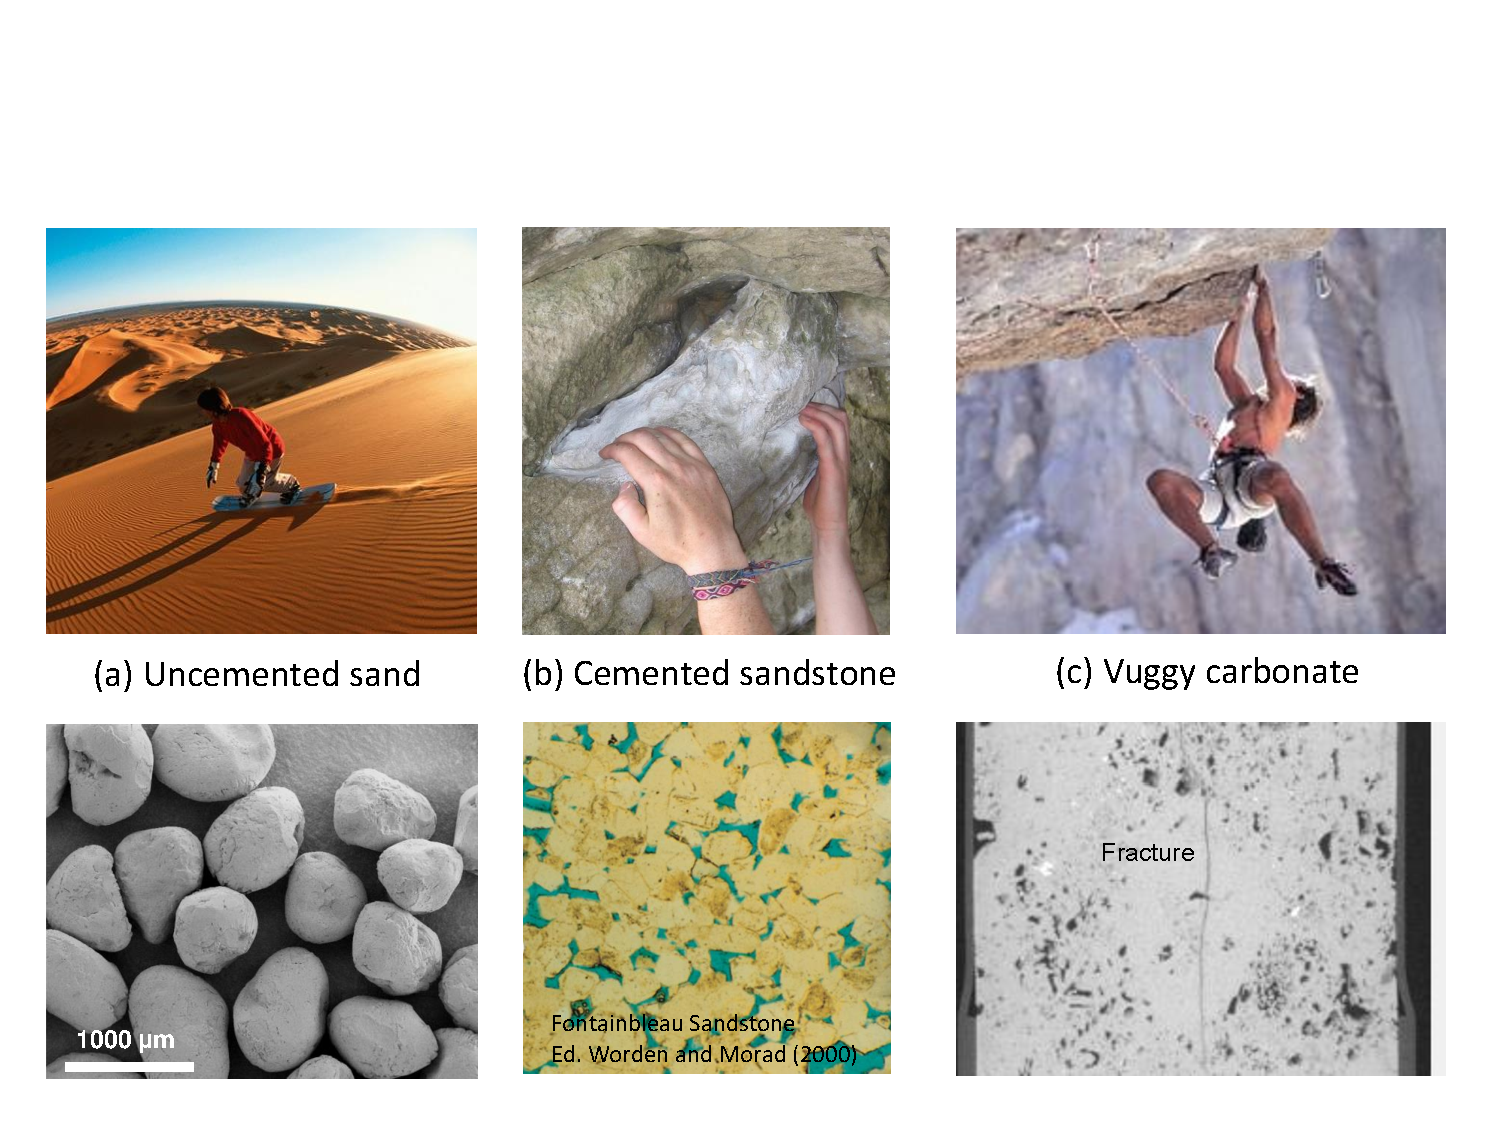
\includegraphics[scale=0.65]{.././Figures/split/5A-3.pdf}%
\lthtmlpictureZ
\lthtmlcheckvsize\clearpage}

\stepcounter{subsection}
{\newpage\clearpage
\lthtmlpictureA{tex2html_wrap16541}%
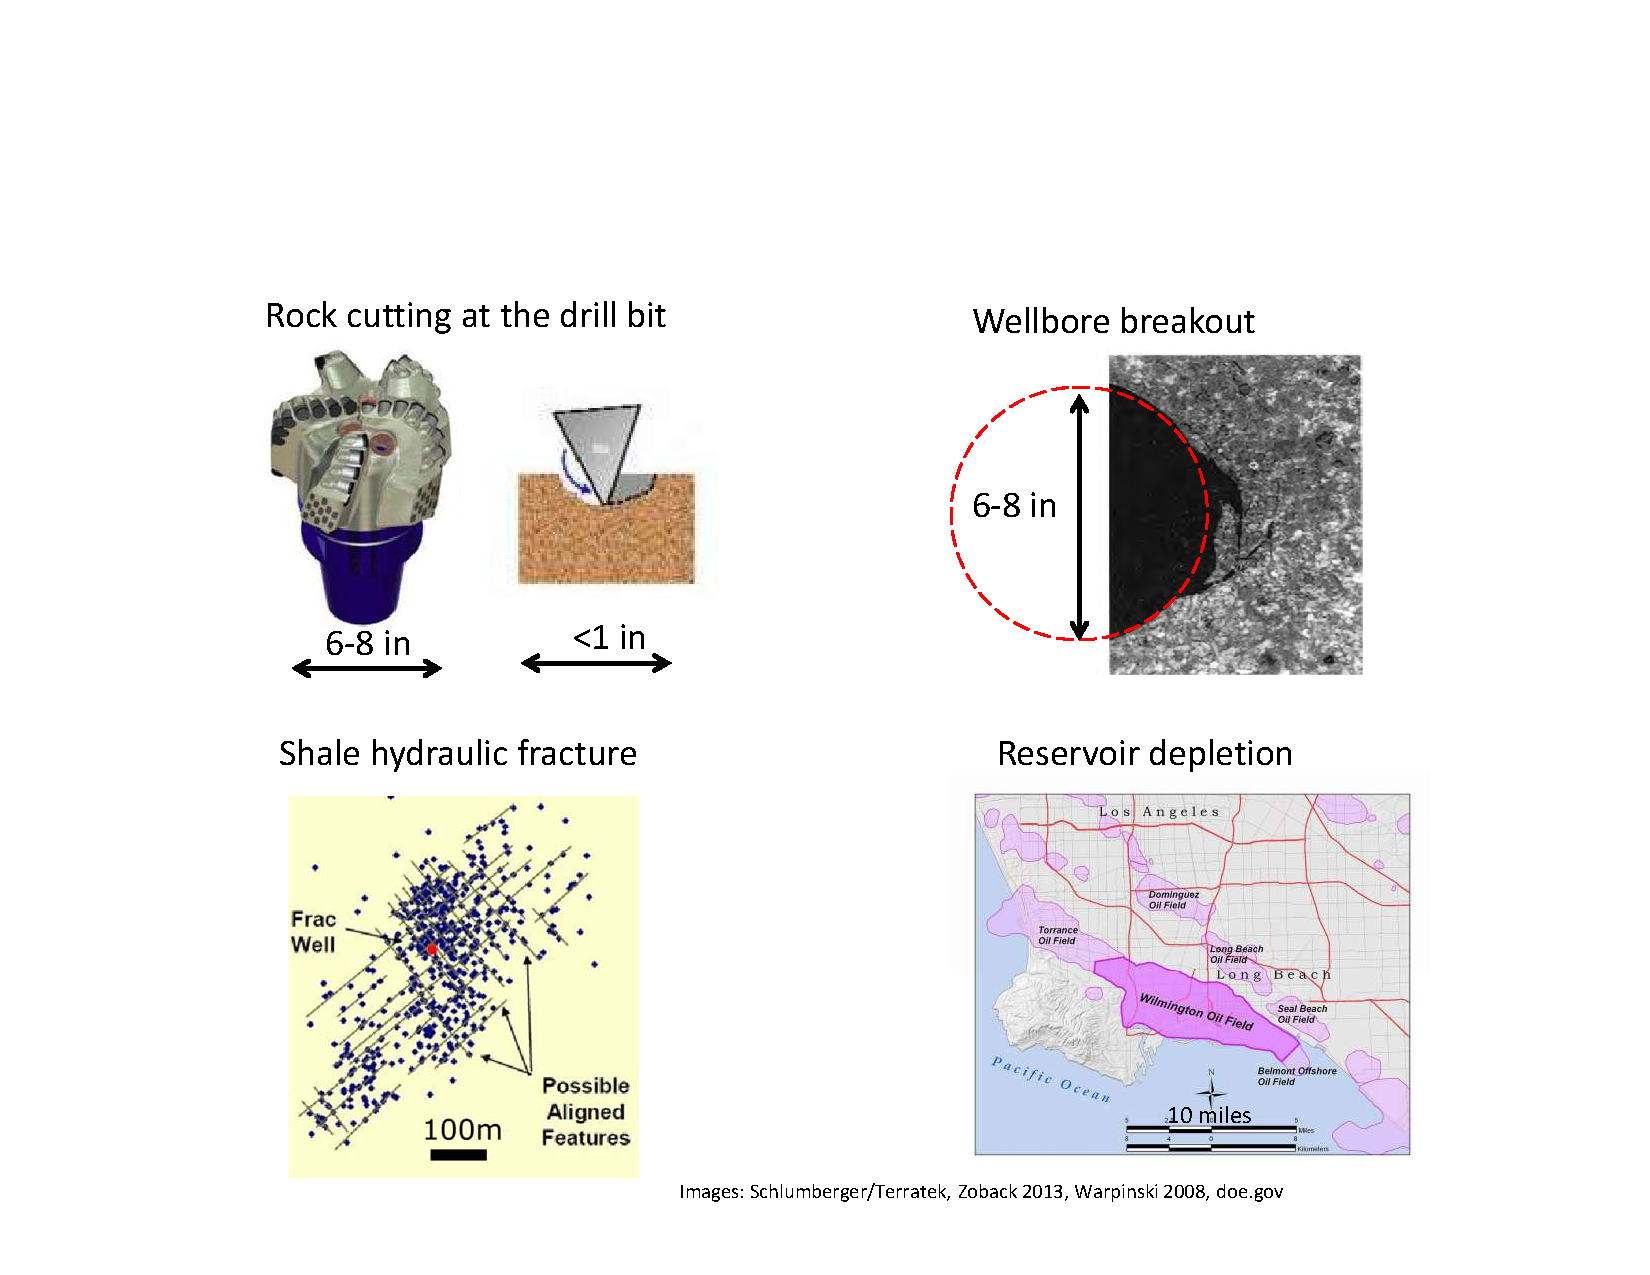
\includegraphics[scale=0.65]{.././Figures/split/5A-4.pdf}%
\lthtmlpictureZ
\lthtmlcheckvsize\clearpage}

\stepcounter{subsection}
{\newpage\clearpage
\lthtmlpictureA{tex2html_wrap16547}%
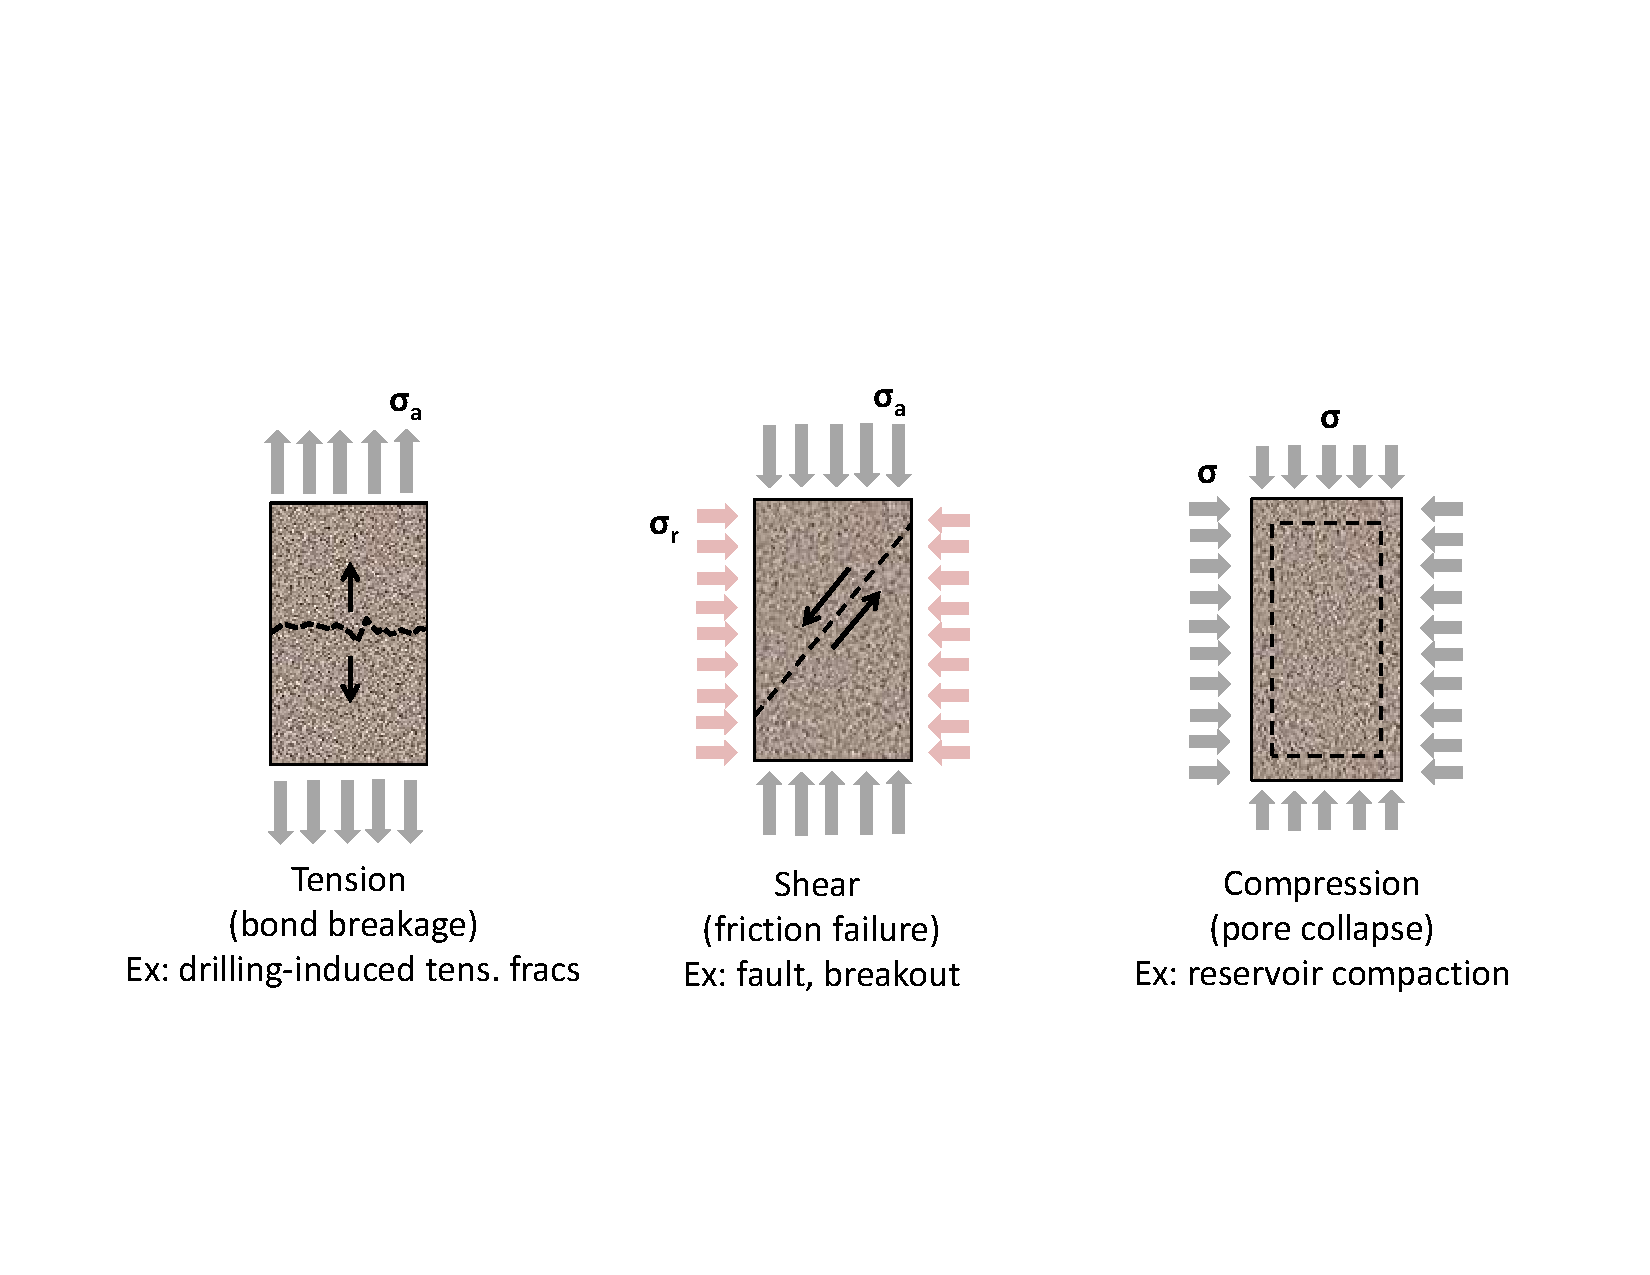
\includegraphics[scale=0.55]{.././Figures/split/5A-5.pdf}%
\lthtmlpictureZ
\lthtmlcheckvsize\clearpage}

\stepcounter{section}
\stepcounter{subsection}
{\newpage\clearpage
\lthtmlpictureA{tex2html_wrap16554}%
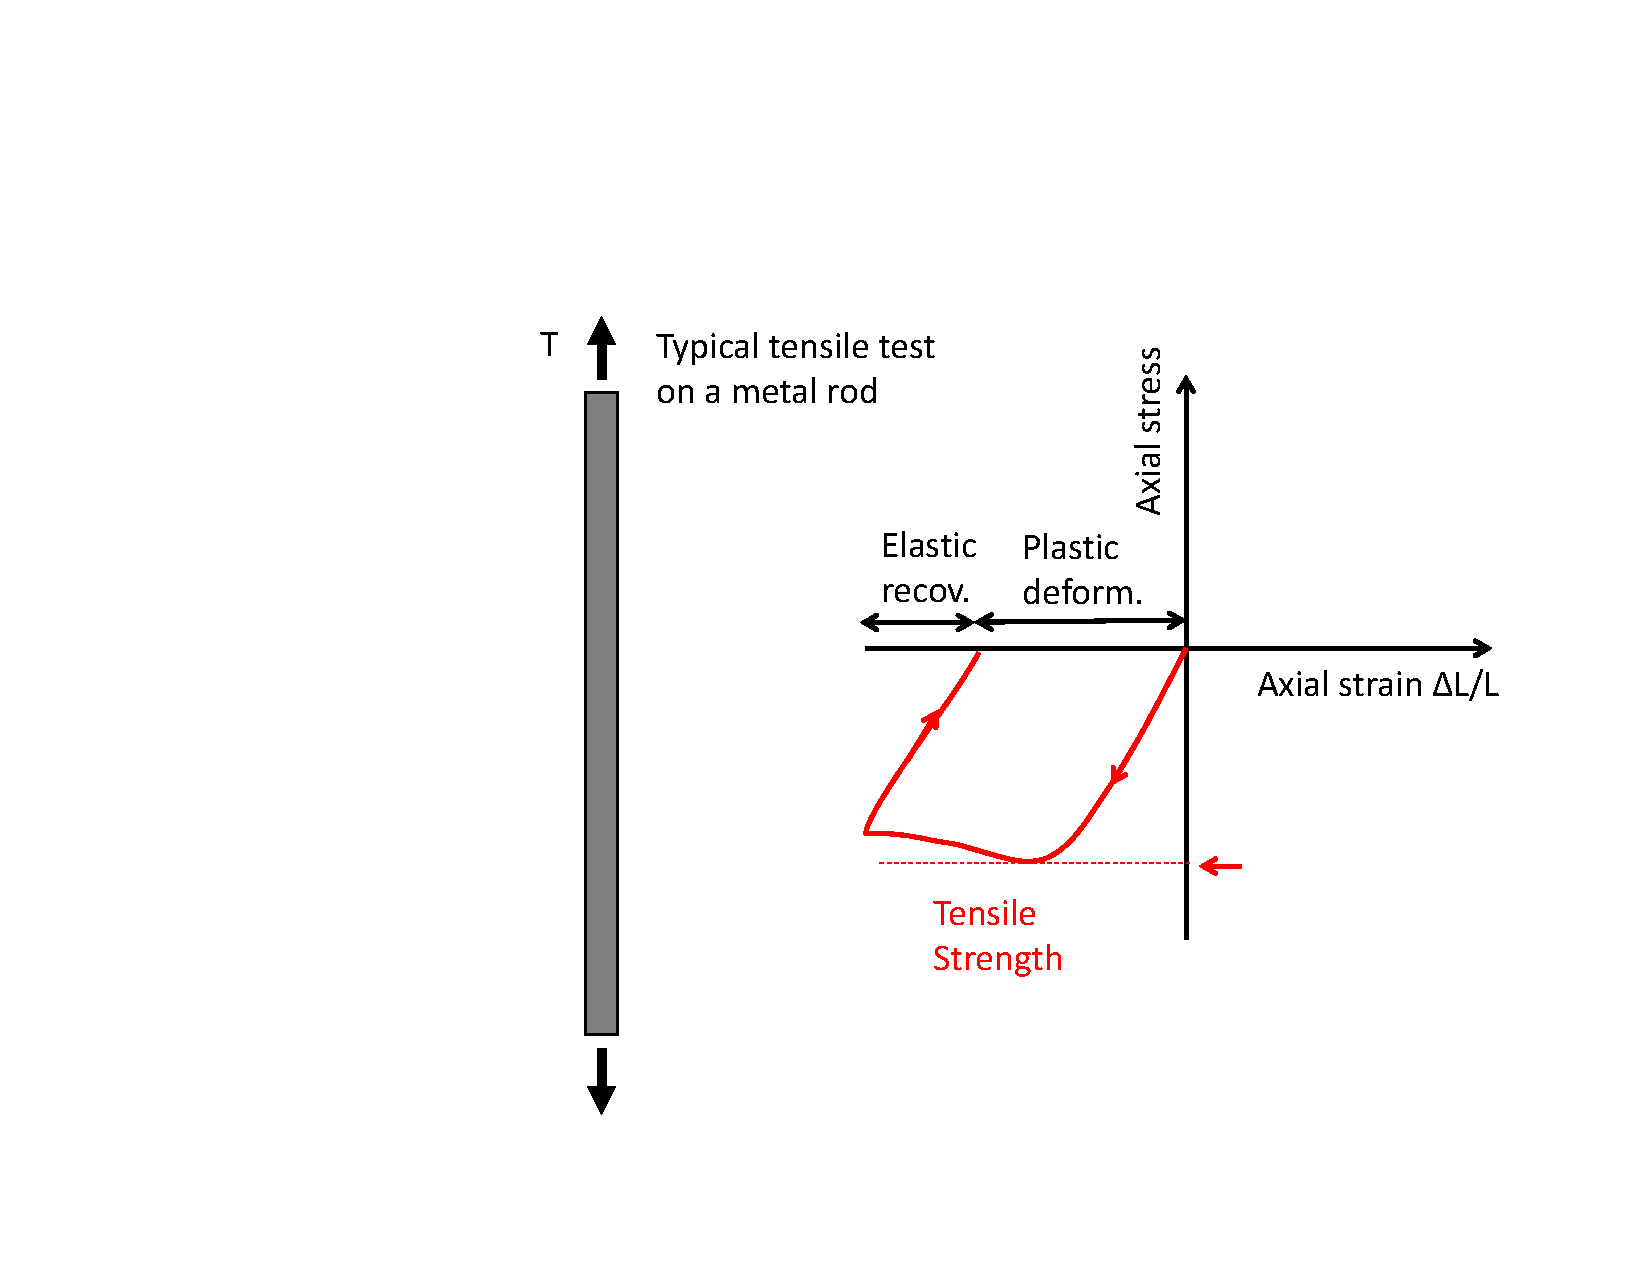
\includegraphics[scale=0.55]{.././Figures/split/5A-6.pdf}%
\lthtmlpictureZ
\lthtmlcheckvsize\clearpage}

{\newpage\clearpage
\lthtmlpictureA{tex2html_wrap16559}%
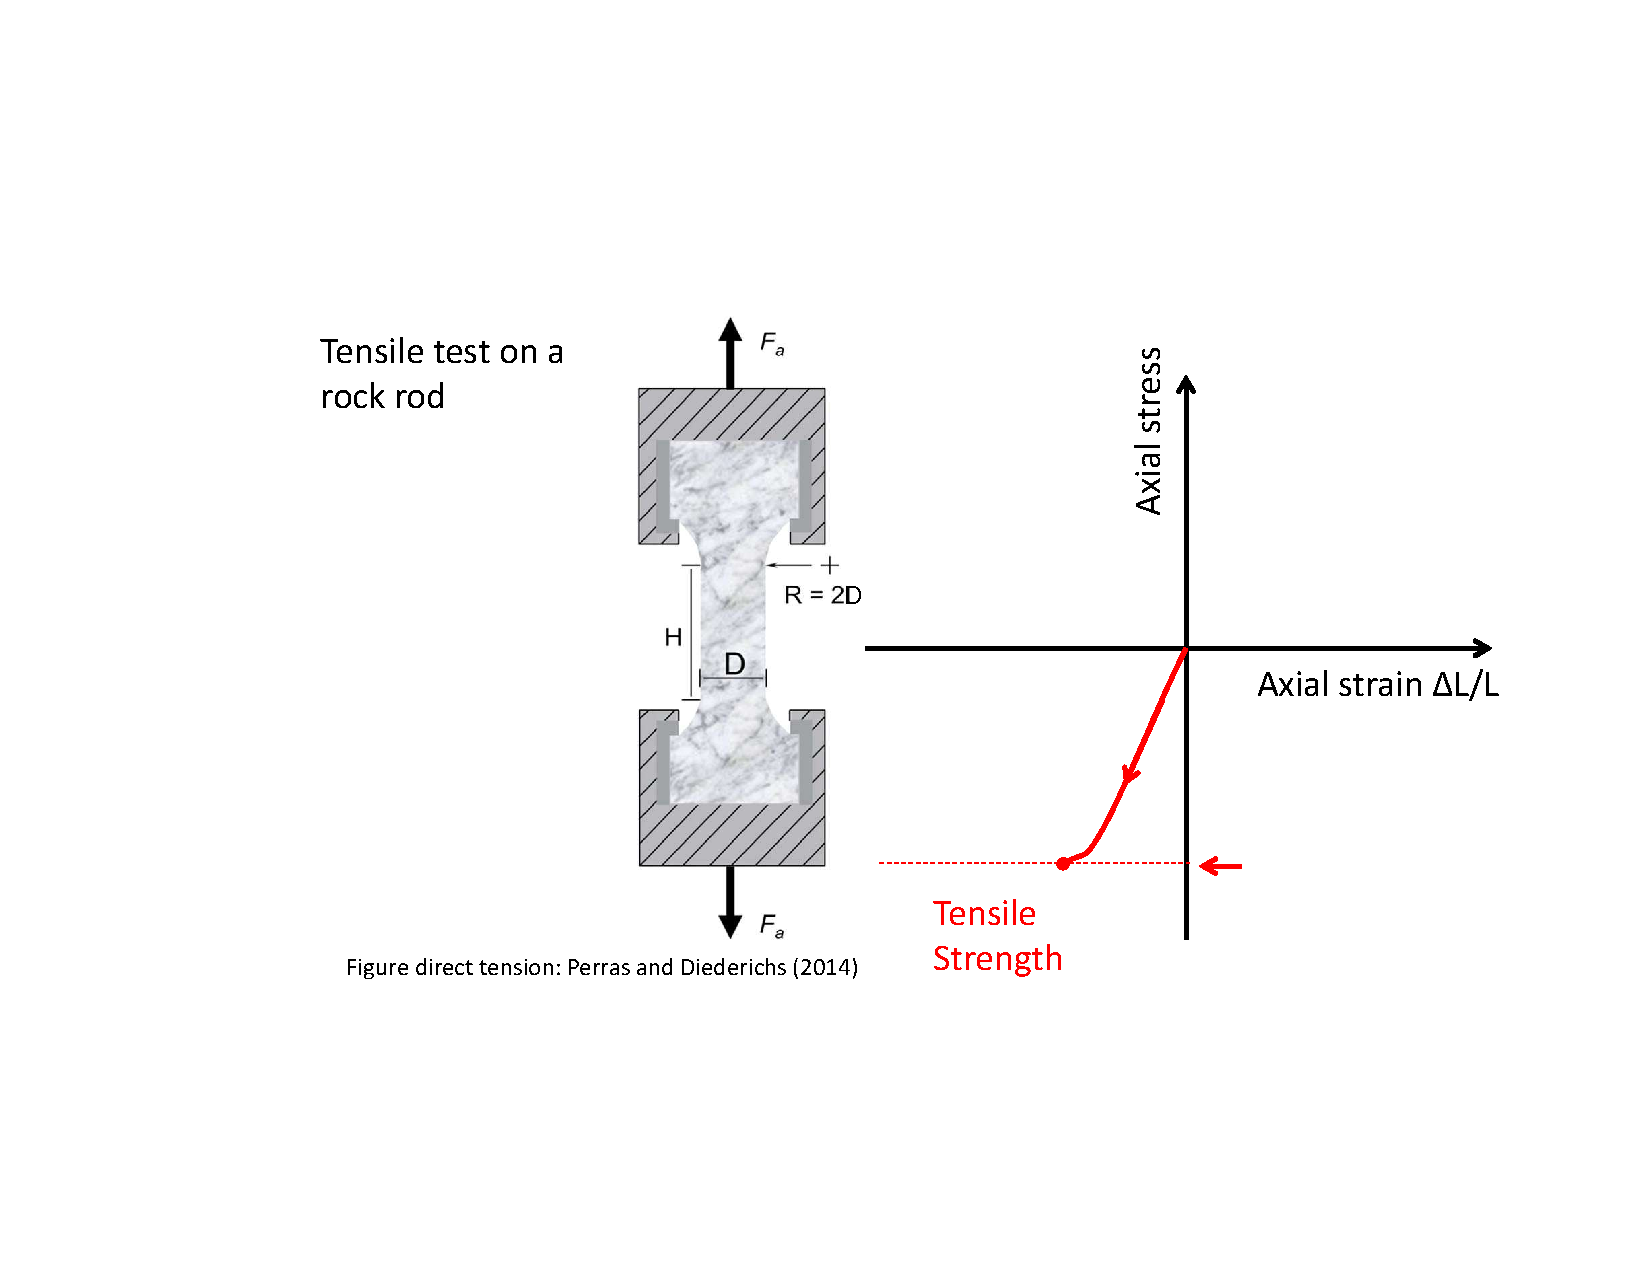
\includegraphics[scale=0.60]{.././Figures/split/5A-7.pdf}%
\lthtmlpictureZ
\lthtmlcheckvsize\clearpage}

\stepcounter{subsection}
{\newpage\clearpage
\lthtmlinlinemathA{tex2html_wrap_inline16565}%
$ T_S$%
\lthtmlindisplaymathZ
\lthtmlcheckvsize\clearpage}

{\newpage\clearpage
\lthtmlinlinemathA{tex2html_wrap_indisplay16567}%
$\displaystyle T_S = \frac{P_B}{\pi L R}$%
\lthtmlindisplaymathZ
\lthtmlcheckvsize\clearpage}

{\newpage\clearpage
\lthtmlinlinemathA{tex2html_wrap_inline16569}%
$ P_B$%
\lthtmlindisplaymathZ
\lthtmlcheckvsize\clearpage}

{\newpage\clearpage
\lthtmlinlinemathA{tex2html_wrap_inline16573}%
$ R$%
\lthtmlindisplaymathZ
\lthtmlcheckvsize\clearpage}

{\newpage\clearpage
\lthtmlpictureA{tex2html_wrap16575}%
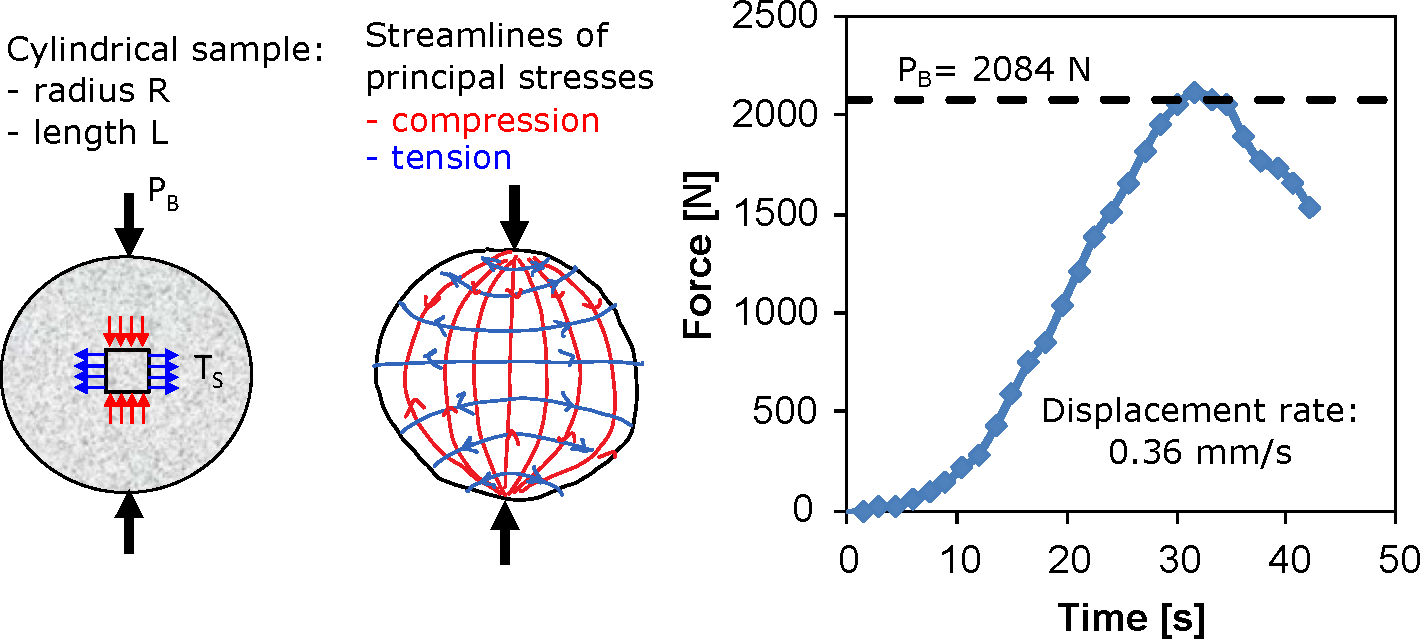
\includegraphics[scale=0.55]{.././Figures/split/4-TensileStrength.pdf}%
\lthtmlpictureZ
\lthtmlcheckvsize\clearpage}

{\newpage\clearpage
\lthtmlinlinemathA{tex2html_wrap_indisplay16580}%
$\displaystyle R = \frac{1}{2}$%
\lthtmlindisplaymathZ
\lthtmlcheckvsize\clearpage}

{\newpage\clearpage
\lthtmlinlinemathA{tex2html_wrap_indisplay16581}%
$\displaystyle = 0.0127$%
\lthtmlindisplaymathZ
\lthtmlcheckvsize\clearpage}

{\newpage\clearpage
\lthtmlinlinemathA{tex2html_wrap_indisplay16583}%
$\displaystyle L = 1$%
\lthtmlindisplaymathZ
\lthtmlcheckvsize\clearpage}

{\newpage\clearpage
\lthtmlinlinemathA{tex2html_wrap_indisplay16584}%
$\displaystyle = 0.0254$%
\lthtmlindisplaymathZ
\lthtmlcheckvsize\clearpage}

{\newpage\clearpage
\lthtmlinlinemathA{tex2html_wrap_indisplay16586}%
$\displaystyle T_S = \frac{2084 \text { N}}{\pi (0.0254 \text{ m}) (0.0127 \text{ m})}
= 2.06 \times 10^6 \text{ Pa} = 2.06 \text{ MPa} \: \: \blacksquare$%
\lthtmlindisplaymathZ
\lthtmlcheckvsize\clearpage}

{\newpage\clearpage
\lthtmlpictureA{tex2html_wrap16588}%
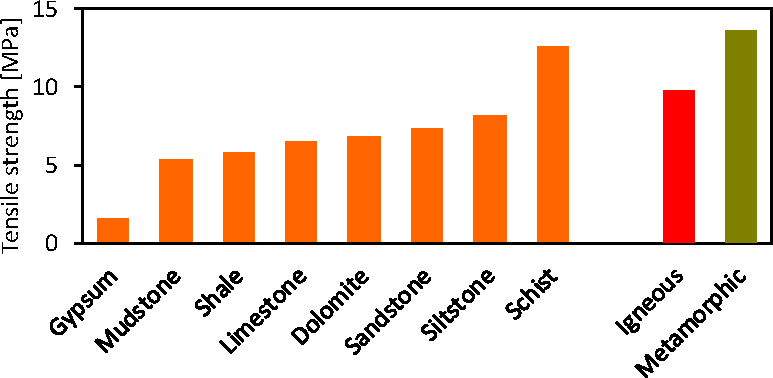
\includegraphics[scale=0.65]{.././Figures/split/4-TensStrengthSummary.pdf}%
\lthtmlpictureZ
\lthtmlcheckvsize\clearpage}

\stepcounter{section}
\stepcounter{subsection}
{\newpage\clearpage
\lthtmlinlinemathA{tex2html_wrap_inline16595}%
$ S_0$%
\lthtmlindisplaymathZ
\lthtmlcheckvsize\clearpage}

{\newpage\clearpage
\lthtmlinlinemathA{tex2html_wrap_inline16597}%
$ F_T$%
\lthtmlindisplaymathZ
\lthtmlcheckvsize\clearpage}

{\newpage\clearpage
\lthtmlinlinemathA{tex2html_wrap_inline16601}%
$ F_N$%
\lthtmlindisplaymathZ
\lthtmlcheckvsize\clearpage}

{\newpage\clearpage
\lthtmlinlinemathA{tex2html_wrap_inline16603}%
$ F_T = \mu F_N$%
\lthtmlindisplaymathZ
\lthtmlcheckvsize\clearpage}

{\newpage\clearpage
\lthtmlinlinemathA{tex2html_wrap_inline16605}%
$ F_N=0$%
\lthtmlindisplaymathZ
\lthtmlcheckvsize\clearpage}

{\newpage\clearpage
\lthtmlinlinemathA{tex2html_wrap_inline16607}%
$ F_T = 0$%
\lthtmlindisplaymathZ
\lthtmlcheckvsize\clearpage}

{\newpage\clearpage
\lthtmlpictureA{tex2html_wrap16613}%
\includegraphics[scale=0.45]{.././Figures/split/5A-10.pdf}%
\lthtmlpictureZ
\lthtmlcheckvsize\clearpage}

{\newpage\clearpage
\lthtmlinlinemathA{tex2html_wrap_inline16618}%
$ \tau$%
\lthtmlindisplaymathZ
\lthtmlcheckvsize\clearpage}

{\newpage\clearpage
\lthtmlinlinemathA{tex2html_wrap_inline16620}%
$ \sigma_n$%
\lthtmlindisplaymathZ
\lthtmlcheckvsize\clearpage}

{\newpage\clearpage
\lthtmlinlinemathA{tex2html_wrap_inline16622}%
$ \mu_i$%
\lthtmlindisplaymathZ
\lthtmlcheckvsize\clearpage}

{\newpage\clearpage
\lthtmlinlinemathA{tex2html_wrap_inline16624}%
$ \tau = \mu_i \sigma_n$%
\lthtmlindisplaymathZ
\lthtmlcheckvsize\clearpage}

{\newpage\clearpage
\lthtmlpictureA{tex2html_wrap16626}%
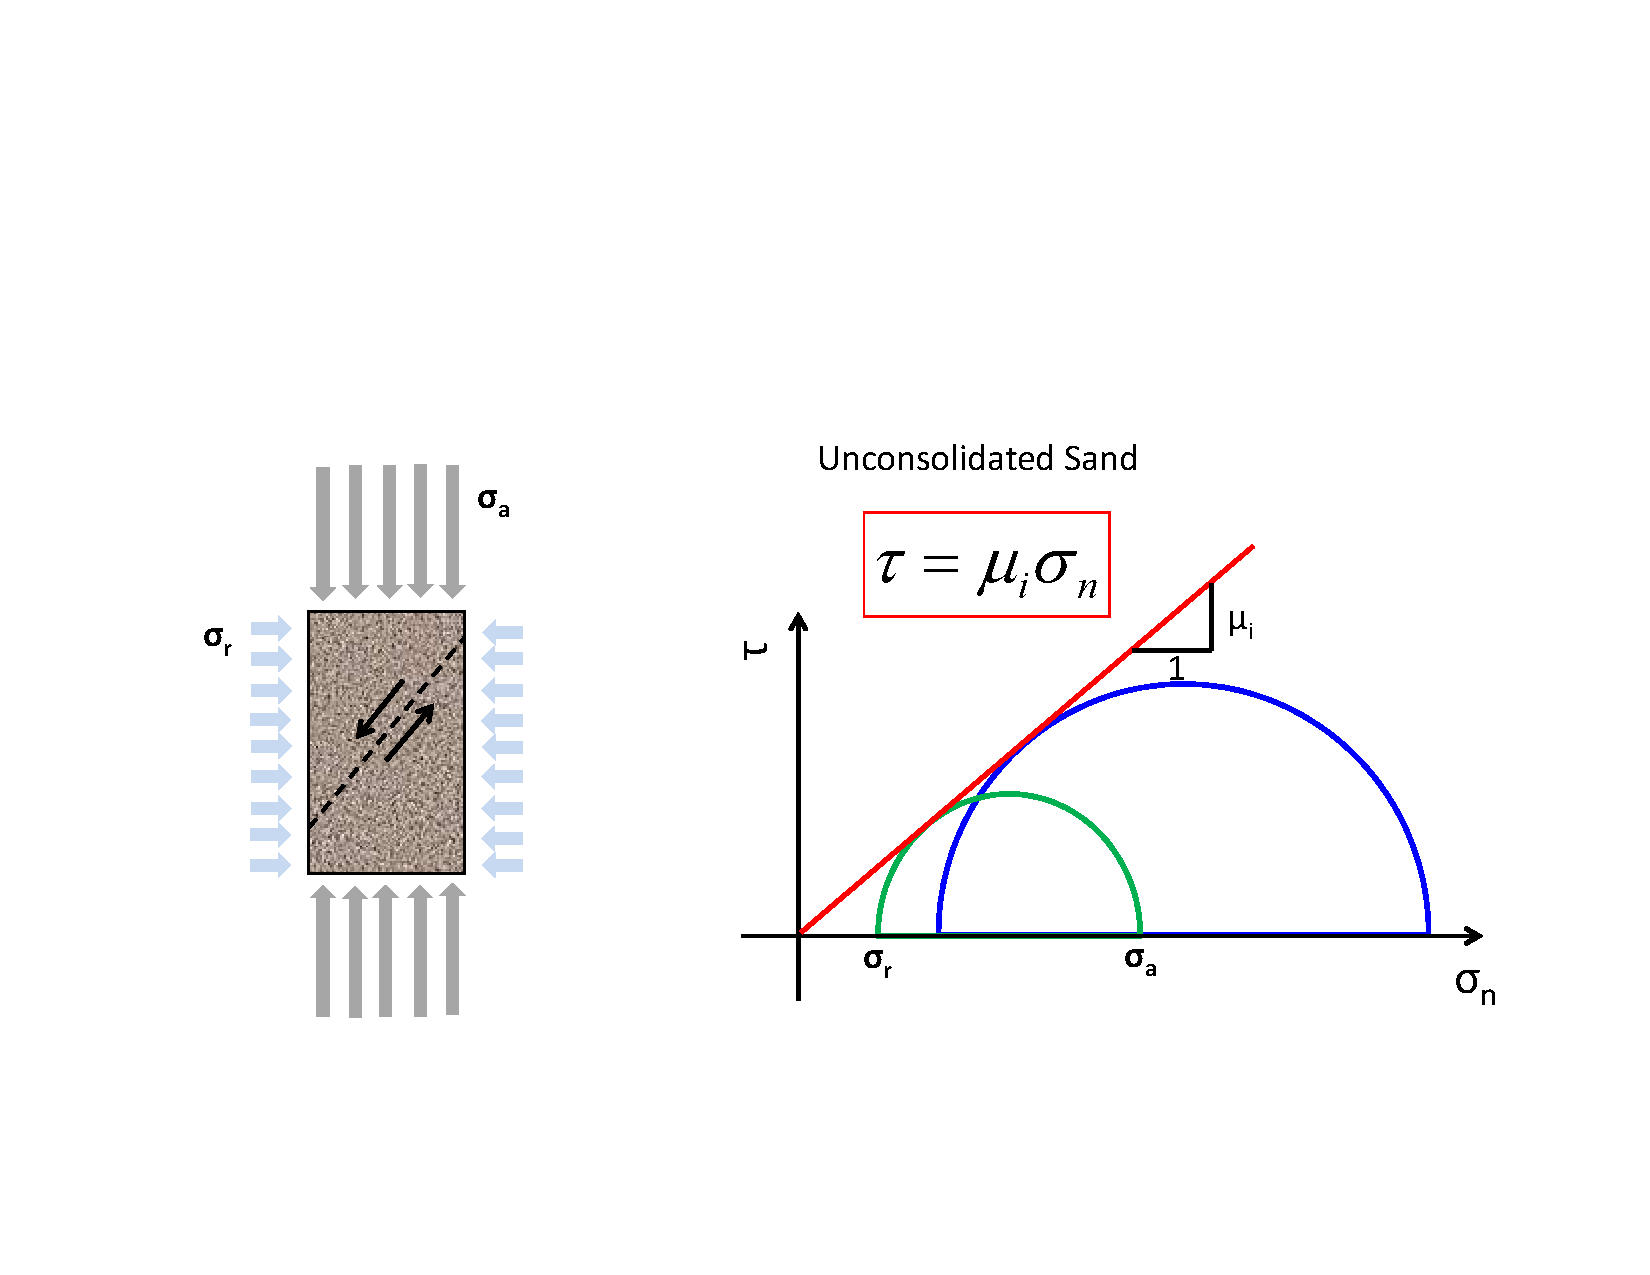
\includegraphics[scale=0.50]{.././Figures/split/5A-14.pdf}%
\lthtmlpictureZ
\lthtmlcheckvsize\clearpage}

{\newpage\clearpage
\lthtmlinlinemathA{tex2html_wrap_inline16637}%
$ \sigma_n = 0$%
\lthtmlindisplaymathZ
\lthtmlcheckvsize\clearpage}

{\newpage\clearpage
\lthtmlinlinemathA{tex2html_wrap_inline16639}%
$ \tau = 0$%
\lthtmlindisplaymathZ
\lthtmlcheckvsize\clearpage}

{\newpage\clearpage
\lthtmlinlinemathA{tex2html_wrap_inline16643}%
$ \varphi$%
\lthtmlindisplaymathZ
\lthtmlcheckvsize\clearpage}

{\newpage\clearpage
\lthtmlinlinemathA{tex2html_wrap_inline16645}%
$ \tan (\varphi) = \mu_i$%
\lthtmlindisplaymathZ
\lthtmlcheckvsize\clearpage}

{\newpage\clearpage
\lthtmlinlinemathA{tex2html_wrap_inline16649}%
$ \mu_i=0.5$%
\lthtmlindisplaymathZ
\lthtmlcheckvsize\clearpage}

{\newpage\clearpage
\lthtmlinlinemathA{tex2html_wrap_inline16651}%
$ \varphi \sim 30^{\circ}$%
\lthtmlindisplaymathZ
\lthtmlcheckvsize\clearpage}

\stepcounter{subsection}
{\newpage\clearpage
\lthtmlinlinemathA{tex2html_wrap_inline16654}%
$ \sigma_r = 0$%
\lthtmlindisplaymathZ
\lthtmlcheckvsize\clearpage}

{\newpage\clearpage
\lthtmlinlinemathA{tex2html_wrap_inline16660}%
$ UCS$%
\lthtmlindisplaymathZ
\lthtmlcheckvsize\clearpage}

{\newpage\clearpage
\lthtmlpictureA{tex2html_wrap16662}%
\includegraphics[scale=0.60]{.././Figures/split/5A-12.pdf}%
\lthtmlpictureZ
\lthtmlcheckvsize\clearpage}

\stepcounter{subsection}
{\newpage\clearpage
\lthtmlinlinemathA{tex2html_wrap_inline16668}%
$ \sigma_r \neq 0$%
\lthtmlindisplaymathZ
\lthtmlcheckvsize\clearpage}

{\newpage\clearpage
\lthtmlinlinemathA{tex2html_wrap_indisplay16676}%
$\displaystyle \tau = S_0 + \mu_i \sigma_n$%
\lthtmlindisplaymathZ
\lthtmlcheckvsize\clearpage}

{\newpage\clearpage
\lthtmlpictureA{tex2html_wrap16678}%
\includegraphics[scale=0.60]{.././Figures/split/5A-13.pdf}%
\lthtmlpictureZ
\lthtmlcheckvsize\clearpage}

{\newpage\clearpage
\lthtmlinlinemathA{tex2html_wrap_inline16687}%
$ \pi/4 + \varphi/2$%
\lthtmlindisplaymathZ
\lthtmlcheckvsize\clearpage}

{\newpage\clearpage
\lthtmlinlinemathA{tex2html_wrap_inline16691}%
$ \pi/4 + \varphi/2 = 60^{\circ}$%
\lthtmlindisplaymathZ
\lthtmlcheckvsize\clearpage}

{\newpage\clearpage
\lthtmlinlinemathA{tex2html_wrap_inline16695}%
$ \sigma_a / \sigma_r$%
\lthtmlindisplaymathZ
\lthtmlcheckvsize\clearpage}

{\newpage\clearpage
\lthtmlpictureA{tex2html_wrap16697}%
\includegraphics[scale=0.50]{.././Figures/split/5A-15.pdf}%
\lthtmlpictureZ
\lthtmlcheckvsize\clearpage}

{\newpage\clearpage
\lthtmlinlinemathA{tex2html_wrap_inline16701}%
$ \tau / \sigma_n = \mu_i$%
\lthtmlindisplaymathZ
\lthtmlcheckvsize\clearpage}

{\newpage\clearpage
\lthtmlpictureA{tex2html_wrap16703}%
\includegraphics[scale=0.55]{.././Figures/split/AngleFailurePlane.pdf}%
\lthtmlpictureZ
\lthtmlcheckvsize\clearpage}

{\newpage\clearpage
\lthtmlinlinemathA{tex2html_wrap_inline16705}%
$ (\sigma_a,0)$%
\lthtmlindisplaymathZ
\lthtmlcheckvsize\clearpage}

{\newpage\clearpage
\lthtmlinlinemathA{tex2html_wrap_inline16711}%
$ (\sigma_r,0)$%
\lthtmlindisplaymathZ
\lthtmlcheckvsize\clearpage}

{\newpage\clearpage
\lthtmlinlinemathA{tex2html_wrap_inline16717}%
$ (\sigma_n,\tau)$%
\lthtmlindisplaymathZ
\lthtmlcheckvsize\clearpage}

{\newpage\clearpage
\lthtmlinlinemathA{tex2html_wrap_inline16719}%
$ \pi/2 + \varphi$%
\lthtmlindisplaymathZ
\lthtmlcheckvsize\clearpage}

{\newpage\clearpage
\lthtmlinlinemathA{tex2html_wrap_inline16725}%
$ (\pi/2 + \varphi)/2$%
\lthtmlindisplaymathZ
\lthtmlcheckvsize\clearpage}

{\newpage\clearpage
\lthtmlinlinemathA{tex2html_wrap_inline16731}%
$ ^{\circ} = \pi/2$%
\lthtmlindisplaymathZ
\lthtmlcheckvsize\clearpage}

{\newpage\clearpage
\lthtmlinlinemathA{tex2html_wrap_inline16733}%
$ C$%
\lthtmlindisplaymathZ
\lthtmlcheckvsize\clearpage}

{\newpage\clearpage
\lthtmlinlinemathA{tex2html_wrap_indisplay16739}%
$\displaystyle \frac{\sigma_a}{\sigma_r} = \frac{C + R}{C-R} = 
		\frac{C+C \sin \varphi}{C-C \sin \varphi} =
		\frac{1+\sin \varphi}{1-\sin \varphi} =		
 \: \: \blacksquare
$%
\lthtmlindisplaymathZ
\lthtmlcheckvsize\clearpage}

{\newpage\clearpage
\lthtmlinlinemathA{tex2html_wrap_indisplay16741}%
$\displaystyle \sigma_1 = UCS + q \: \sigma_3$%
\lthtmlindisplaymathZ
\lthtmlcheckvsize\clearpage}

{\newpage\clearpage
\lthtmlinlinemathA{tex2html_wrap_inline16743}%
$ \sigma_1$%
\lthtmlindisplaymathZ
\lthtmlcheckvsize\clearpage}

{\newpage\clearpage
\lthtmlinlinemathA{tex2html_wrap_inline16745}%
$ \sigma_3$%
\lthtmlindisplaymathZ
\lthtmlcheckvsize\clearpage}

{\newpage\clearpage
\lthtmlinlinemathA{tex2html_wrap_inline16747}%
$ q$%
\lthtmlindisplaymathZ
\lthtmlcheckvsize\clearpage}

{\newpage\clearpage
\lthtmlinlinemathA{tex2html_wrap_inline16751}%
$ p'-q$%
\lthtmlindisplaymathZ
\lthtmlcheckvsize\clearpage}

{\newpage\clearpage
\lthtmlinlinemathA{tex2html_wrap_inline16753}%
$ \sigma_m-q$%
\lthtmlindisplaymathZ
\lthtmlcheckvsize\clearpage}

{\newpage\clearpage
\lthtmlinlinemathA{tex2html_wrap_indisplay16755}%
$\displaystyle q = \frac{1 + \sin \varphi}{1 - \sin \varphi}$%
\lthtmlindisplaymathZ
\lthtmlcheckvsize\clearpage}

{\newpage\clearpage
\lthtmlinlinemathA{tex2html_wrap_inline16757}%
$ \varphi ~ 30^{\circ}$%
\lthtmlindisplaymathZ
\lthtmlcheckvsize\clearpage}

{\newpage\clearpage
\lthtmlinlinemathA{tex2html_wrap_inline16759}%
$ q = 3$%
\lthtmlindisplaymathZ
\lthtmlcheckvsize\clearpage}

{\newpage\clearpage
\lthtmlinlinemathA{tex2html_wrap_indisplay16763}%
$\displaystyle UCS = 2 S_0 \left( \frac{1 + \sin \varphi}{1 - \sin \varphi} \right)^{1/2}
= 2 S_0 \sqrt{q}$%
\lthtmlindisplaymathZ
\lthtmlcheckvsize\clearpage}

{\newpage\clearpage
\lthtmlpictureA{tex2html_wrap16765}%
\includegraphics[scale=0.65]{.././Figures/split/5A-16.pdf}%
\lthtmlpictureZ
\lthtmlcheckvsize\clearpage}

{\newpage\clearpage
\lthtmlpictureA{tex2html_wrap16770}%
\includegraphics[scale=0.85]{.././Figures/split/4-ShearStrengthSummary.pdf}%
\lthtmlpictureZ
\lthtmlcheckvsize\clearpage}

\stepcounter{subsection}
{\newpage\clearpage
\lthtmlinlinemathA{tex2html_wrap_inline16776}%
$ (S_1,S_2,S_3)$%
\lthtmlindisplaymathZ
\lthtmlcheckvsize\clearpage}

{\newpage\clearpage
\lthtmlinlinemathA{tex2html_wrap_inline16778}%
$ (\sigma_1,\sigma_2,\sigma_3)$%
\lthtmlindisplaymathZ
\lthtmlcheckvsize\clearpage}

{\newpage\clearpage
\lthtmlinlinemathA{tex2html_wrap_inline16780}%
$ P_c$%
\lthtmlindisplaymathZ
\lthtmlcheckvsize\clearpage}

{\newpage\clearpage
\lthtmlinlinemathA{tex2html_wrap_inline16782}%
$ \sigma_D$%
\lthtmlindisplaymathZ
\lthtmlcheckvsize\clearpage}

{\newpage\clearpage
\lthtmlinlinemathA{tex2html_wrap_inline16788}%
$ P_c = cst$%
\lthtmlindisplaymathZ
\lthtmlcheckvsize\clearpage}

{\newpage\clearpage
\lthtmlinlinemathA{tex2html_wrap_inline16792}%
$ P_p < P_c$%
\lthtmlindisplaymathZ
\lthtmlcheckvsize\clearpage}

{\newpage\clearpage
\lthtmlinlinemathA{tex2html_wrap_inline16794}%
$ P_p = cst$%
\lthtmlindisplaymathZ
\lthtmlcheckvsize\clearpage}

{\newpage\clearpage
\lthtmlinlinemathA{tex2html_wrap_inline16798}%
$ \sigma_D =S_1 - S_3$%
\lthtmlindisplaymathZ
\lthtmlcheckvsize\clearpage}

{\newpage\clearpage
\lthtmlinlinemathA{tex2html_wrap_inline16804}%
$ S_3 = P_c$%
\lthtmlindisplaymathZ
\lthtmlcheckvsize\clearpage}

{\newpage\clearpage
\lthtmlinlinemathA{tex2html_wrap_inline16806}%
$ S_2=S_3$%
\lthtmlindisplaymathZ
\lthtmlcheckvsize\clearpage}

{\newpage\clearpage
\lthtmlinlinemathA{tex2html_wrap_inline16808}%
$ S_1 - S_3=\sigma_1-\sigma_3$%
\lthtmlindisplaymathZ
\lthtmlcheckvsize\clearpage}

{\newpage\clearpage
\lthtmlinlinemathA{tex2html_wrap_inline16810}%
$ d \varepsilon_a / dt = cst$%
\lthtmlindisplaymathZ
\lthtmlcheckvsize\clearpage}

{\newpage\clearpage
\lthtmlinlinemathA{tex2html_wrap_inline16816}%
$ P$%
\lthtmlindisplaymathZ
\lthtmlcheckvsize\clearpage}

{\newpage\clearpage
\lthtmlinlinemathA{tex2html_wrap_inline16824}%
$ \sigma_1 = (S_1 - P_p)$%
\lthtmlindisplaymathZ
\lthtmlcheckvsize\clearpage}

{\newpage\clearpage
\lthtmlinlinemathA{tex2html_wrap_inline16826}%
$ \sigma_3 = (S_3 - P_p)$%
\lthtmlindisplaymathZ
\lthtmlcheckvsize\clearpage}

{\newpage\clearpage
\lthtmlinlinemathA{tex2html_wrap_indisplay16836}%
$\displaystyle \varphi = \arctan \left( \frac{q-1}{2\sqrt{q}} \right)$%
\lthtmlindisplaymathZ
\lthtmlcheckvsize\clearpage}

{\newpage\clearpage
\lthtmlinlinemathA{tex2html_wrap_inline16848}%
$ S_3 \leqslant 80$%
\lthtmlindisplaymathZ
\lthtmlcheckvsize\clearpage}

{\newpage\clearpage
\lthtmlinlinemathA{tex2html_wrap_inline16850}%
$ S_1 \sim 80$%
\lthtmlindisplaymathZ
\lthtmlcheckvsize\clearpage}

{\newpage\clearpage
\lthtmlinlinemathA{tex2html_wrap_indisplay16852}%
$\displaystyle UCS = 80$%
\lthtmlindisplaymathZ
\lthtmlcheckvsize\clearpage}

{\newpage\clearpage
\lthtmlinlinemathA{tex2html_wrap_indisplay16853}%
$\displaystyle $%
\lthtmlindisplaymathZ
\lthtmlcheckvsize\clearpage}

{\newpage\clearpage
\lthtmlinlinemathA{tex2html_wrap_indisplay16857}%
$\displaystyle q = \frac{\Delta \sigma_1}{\Delta \sigma_3} = 
       \frac{520 \text{ MPa}}{110 \text{ MPa}} = 4.73
$%
\lthtmlindisplaymathZ
\lthtmlcheckvsize\clearpage}

{\newpage\clearpage
\lthtmlinlinemathA{tex2html_wrap_indisplay16859}%
$\displaystyle S_0 = \frac{UCS}{2 \sqrt{q}} = \frac{80 \text{MPa}}{2 \sqrt{4.73}} = 18.4 \text{MPa} $%
\lthtmlindisplaymathZ
\lthtmlcheckvsize\clearpage}

{\newpage\clearpage
\lthtmlinlinemathA{tex2html_wrap_indisplay16861}%
$\displaystyle \varphi = \arctan \left( \frac{q-1}{2\sqrt{q}} \right) 
        = \arctan \left( \frac{4.73-1}{2\sqrt{4.73}} \right) = 45.1^{\circ} \: \: \blacksquare
$%
\lthtmlindisplaymathZ
\lthtmlcheckvsize\clearpage}

{\newpage\clearpage
\lthtmlinlinemathA{tex2html_wrap_indisplay16863}%
$\displaystyle \mu_i = \tan (\varphi) = \tan (45.1^{\circ}) = 0.86 
\: \: \blacksquare
$%
\lthtmlindisplaymathZ
\lthtmlcheckvsize\clearpage}

{\newpage\clearpage
\lthtmlinlinemathA{tex2html_wrap_inline16865}%
$ \varepsilon_v = \varepsilon_a + 2\varepsilon_r$%
\lthtmlindisplaymathZ
\lthtmlcheckvsize\clearpage}

{\newpage\clearpage
\lthtmlinlinemathA{tex2html_wrap_inline16867}%
$ d \varepsilon_v/dt<0$%
\lthtmlindisplaymathZ
\lthtmlcheckvsize\clearpage}

{\newpage\clearpage
\lthtmlpictureA{tex2html_wrap16869}%
\includegraphics[scale=0.65]{.././Figures/split/Triaxial-Darley.pdf}%
\lthtmlpictureZ
\lthtmlcheckvsize\clearpage}

\stepcounter{section}
{\newpage\clearpage
\lthtmlpictureA{tex2html_wrap16877}%
\includegraphics[scale=0.65]{.././Figures/split/5A-21.pdf}%
\lthtmlpictureZ
\lthtmlcheckvsize\clearpage}

\stepcounter{section}
{\newpage\clearpage
\lthtmlinlinemathA{tex2html_wrap_inline16891}%
$ \tau = S_0 + \mu_i \sigma_n$%
\lthtmlindisplaymathZ
\lthtmlcheckvsize\clearpage}

{\newpage\clearpage
\lthtmlpictureA{tex2html_wrap16893}%
\includegraphics[scale=0.55]{.././Figures/split/5B-YieldLocus.pdf}%
\lthtmlpictureZ
\lthtmlcheckvsize\clearpage}

\stepcounter{section}
{\newpage\clearpage
\lthtmlinlinemathA{tex2html_wrap_inline16899}%
$ \beta_w$%
\lthtmlindisplaymathZ
\lthtmlcheckvsize\clearpage}

{\newpage\clearpage
\lthtmlinlinemathA{tex2html_wrap_inline16903}%
$ S_w + \mu_w \sigma_n$%
\lthtmlindisplaymathZ
\lthtmlcheckvsize\clearpage}

{\newpage\clearpage
\lthtmlpictureA{tex2html_wrap16905}%
\includegraphics[scale=0.75]{.././Figures/split/5B-8.pdf}%
\lthtmlpictureZ
\lthtmlcheckvsize\clearpage}

\stepcounter{section}
{\newpage\clearpage
\lthtmlpictureA{tex2html_wrap16911}%
\includegraphics[scale=0.65]{.././Figures/split/5B-9.pdf}%
\lthtmlpictureZ
\lthtmlcheckvsize\clearpage}

{\newpage\clearpage
\lthtmlpictureA{tex2html_wrap16916}%
\includegraphics[scale=0.65]{.././Figures/split/5B-10.pdf}%
\lthtmlpictureZ
\lthtmlcheckvsize\clearpage}

{\newpage\clearpage
\lthtmlinlinemathA{tex2html_wrap_inline16921}%
$ \sigma_d = (\sigma_1 - \sigma_3)$%
\lthtmlindisplaymathZ
\lthtmlcheckvsize\clearpage}

{\newpage\clearpage
\lthtmlinlinemathA{tex2html_wrap_inline16923}%
$ \uuline{\varepsilon}{}_p$%
\lthtmlindisplaymathZ
\lthtmlcheckvsize\clearpage}

{\newpage\clearpage
\lthtmlinlinemathA{tex2html_wrap_inline16925}%
$ \uuline{C}{}_p$%
\lthtmlindisplaymathZ
\lthtmlcheckvsize\clearpage}

{\newpage\clearpage
\lthtmlinlinemathA{tex2html_wrap_indisplay16927}%
$\displaystyle \Delta \uuline{\sigma} = \uuline{C}{}_p \Delta \uuline{\varepsilon}{}_p$%
\lthtmlindisplaymathZ
\lthtmlcheckvsize\clearpage}

{\newpage\clearpage
\lthtmlpictureA{tex2html_wrap16929}%
\includegraphics[scale=0.60]{.././Figures/split/5B-11.pdf}%
\lthtmlpictureZ
\lthtmlcheckvsize\clearpage}

\stepcounter{section}
{\newpage\clearpage
\lthtmlpictureA{tex2html_wrap16935}%
\includegraphics[scale=0.65]{.././Figures/split/5B-12.pdf}%
\lthtmlpictureZ
\lthtmlcheckvsize\clearpage}

{\newpage\clearpage
\lthtmlpictureA{tex2html_wrap16940}%
\includegraphics[scale=0.60]{.././Figures/split/5B-13.pdf}%
\lthtmlpictureZ
\lthtmlcheckvsize\clearpage}

{\newpage\clearpage
\lthtmlpictureA{tex2html_wrap16945}%
\includegraphics[scale=0.55]{.././Figures/split/5B-14.pdf}%
\lthtmlpictureZ
\lthtmlcheckvsize\clearpage}

\stepcounter{section}
{\newpage\clearpage
\lthtmlinlinemathA{tex2html_wrap_inline16955}%
$ S_1 - S_3$%
\lthtmlindisplaymathZ
\lthtmlcheckvsize\clearpage}

{\newpage\clearpage
\lthtmlinlinemathA{tex2html_wrap_inline16981}%
$ \varphi = f(q)$%
\lthtmlindisplaymathZ
\lthtmlcheckvsize\clearpage}

{\newpage\clearpage
\lthtmlinlinemathA{tex2html_wrap_inline16987}%
$ Sig_D$%
\lthtmlindisplaymathZ
\lthtmlcheckvsize\clearpage}

{\newpage\clearpage
\lthtmlinlinemathA{tex2html_wrap_inline16991}%
$ E_x$%
\lthtmlindisplaymathZ
\lthtmlcheckvsize\clearpage}

{\newpage\clearpage
\lthtmlinlinemathA{tex2html_wrap_inline16993}%
$ E_y$%
\lthtmlindisplaymathZ
\lthtmlcheckvsize\clearpage}

{\newpage\clearpage
\lthtmlinlinemathA{tex2html_wrap_inline16995}%
$ q=5.3$%
\lthtmlindisplaymathZ
\lthtmlcheckvsize\clearpage}

{\newpage\clearpage
\lthtmlinlinemathA{tex2html_wrap_inline17001}%
$ S_1=S_3 \rightarrow S_1-S_3=0$%
\lthtmlindisplaymathZ
\lthtmlcheckvsize\clearpage}

{\newpage\clearpage
\lthtmlinlinemathA{tex2html_wrap_inline17062}%
$ S_o$%
\lthtmlindisplaymathZ
\lthtmlcheckvsize\clearpage}

\stepcounter{section}
\stepcounter{chapter}
\stepcounter{section}
{\newpage\clearpage
\lthtmlpictureA{tex2html_wrap17073}%
\includegraphics[scale=0.60]{.././Figures/split/6-2.pdf}%
\lthtmlpictureZ
\lthtmlcheckvsize\clearpage}

\stepcounter{section}
{\newpage\clearpage
\lthtmlpictureA{tex2html_wrap17079}%
\includegraphics[scale=0.60]{.././Figures/split/6-8.pdf}%
\lthtmlpictureZ
\lthtmlcheckvsize\clearpage}

\stepcounter{subsection}
{\newpage\clearpage
\lthtmlinlinemathA{tex2html_wrap_inline17089}%
$ dip$%
\lthtmlindisplaymathZ
\lthtmlcheckvsize\clearpage}

{\newpage\clearpage
\lthtmlpictureA{tex2html_wrap17115}%
\includegraphics[scale=0.65]{.././Figures/split/6-5.pdf}%
\lthtmlpictureZ
\lthtmlcheckvsize\clearpage}

\stepcounter{subsection}
\stepcounter{subsection}
{\newpage\clearpage
\lthtmlpictureA{tex2html_wrap17148}%
\includegraphics[scale=0.55]{.././Figures/split/6-7.pdf}%
\lthtmlpictureZ
\lthtmlcheckvsize\clearpage}

\stepcounter{section}
\stepcounter{subsection}
{\newpage\clearpage
\lthtmlinlinemathA{tex2html_wrap_indisplay17169}%
$\displaystyle \sigma_1 = q \: \sigma_3$%
\lthtmlindisplaymathZ
\lthtmlcheckvsize\clearpage}

{\newpage\clearpage
\lthtmlinlinemathA{tex2html_wrap_indisplay17171}%
$\displaystyle q = \left( \sqrt{\mu^2 +1} + \mu \right) ^2 = \frac{1+\sin \: \varphi}{1-\sin \: \varphi}$%
\lthtmlindisplaymathZ
\lthtmlcheckvsize\clearpage}

{\newpage\clearpage
\lthtmlinlinemathA{tex2html_wrap_inline17175}%
$ \sigma_1/\sigma_3 \sim $%
\lthtmlindisplaymathZ
\lthtmlcheckvsize\clearpage}

{\newpage\clearpage
\lthtmlpictureA{tex2html_wrap17177}%
\includegraphics[scale=0.65]{.././Figures/split/6-20.pdf}%
\lthtmlpictureZ
\lthtmlcheckvsize\clearpage}

{\newpage\clearpage
\lthtmlinlinemathA{tex2html_wrap_inline17191}%
$ \pi/4 + \phi/2$%
\lthtmlindisplaymathZ
\lthtmlcheckvsize\clearpage}

{\newpage\clearpage
\lthtmlinlinemathA{tex2html_wrap_inline17193}%
$ \sim 30 ^{\circ}$%
\lthtmlindisplaymathZ
\lthtmlcheckvsize\clearpage}

{\newpage\clearpage
\lthtmlinlinemathA{tex2html_wrap_inline17195}%
$ \sim 60 ^{\circ}$%
\lthtmlindisplaymathZ
\lthtmlcheckvsize\clearpage}

{\newpage\clearpage
\lthtmlinlinemathA{tex2html_wrap_inline17197}%
$ 45 ^{\circ}$%
\lthtmlindisplaymathZ
\lthtmlcheckvsize\clearpage}

{\newpage\clearpage
\lthtmlinlinemathA{tex2html_wrap_inline17199}%
$ 67.5 ^{\circ}$%
\lthtmlindisplaymathZ
\lthtmlcheckvsize\clearpage}

{\newpage\clearpage
\lthtmlinlinemathA{tex2html_wrap_inline17201}%
$ 50 ^{\circ}$%
\lthtmlindisplaymathZ
\lthtmlcheckvsize\clearpage}

{\newpage\clearpage
\lthtmlinlinemathA{tex2html_wrap_inline17203}%
$ 70 ^{\circ}$%
\lthtmlindisplaymathZ
\lthtmlcheckvsize\clearpage}

{\newpage\clearpage
\lthtmlinlinemathA{tex2html_wrap_inline17221}%
$ \sigma_1 / \sigma_3 > q$%
\lthtmlindisplaymathZ
\lthtmlcheckvsize\clearpage}

{\newpage\clearpage
\lthtmlinlinemathA{tex2html_wrap_inline17223}%
$ \sigma_1 / \sigma_3 < q$%
\lthtmlindisplaymathZ
\lthtmlcheckvsize\clearpage}

\stepcounter{subsection}
{\newpage\clearpage
\lthtmldisplayA{displaymath17226}%
\begin{displaymath}\left\lbrace
\begin{array}{l}
S_1 = S_v \\
S_2 = S_{Hmax} \\
S_3 = S_{hmin} \\
\end{array}
\right.\end{displaymath}%
\lthtmldisplayZ
\lthtmlcheckvsize\clearpage}

{\newpage\clearpage
\lthtmlinlinemathA{tex2html_wrap_inline17228}%
$ S_1 > S_2 > S_3$%
\lthtmlindisplaymathZ
\lthtmlcheckvsize\clearpage}

{\newpage\clearpage
\lthtmlpictureA{tex2html_wrap17240}%
\includegraphics[scale=0.50]{.././Figures/split/6-12.pdf}%
\lthtmlpictureZ
\lthtmlcheckvsize\clearpage}

{\newpage\clearpage
\lthtmlinlinemathA{tex2html_wrap_inline17245}%
$ S_1 \neq S_2 \neq S_3$%
\lthtmlindisplaymathZ
\lthtmlcheckvsize\clearpage}

{\newpage\clearpage
\lthtmlpictureA{tex2html_wrap17247}%
\includegraphics[scale=0.55]{.././Figures/split/6-13.pdf}%
\lthtmlpictureZ
\lthtmlcheckvsize\clearpage}

\stepcounter{subsection}
{\newpage\clearpage
\lthtmldisplayA{displaymath17253}%
\begin{displaymath}\left\lbrace
\begin{array}{l}
S_1 = S_{Hmax} \\
S_2 = S_{hmin} \\
S_3 = S_v \\
\end{array}
\right.\end{displaymath}%
\lthtmldisplayZ
\lthtmlcheckvsize\clearpage}

{\newpage\clearpage
\lthtmlinlinemathA{tex2html_wrap_inline17255}%
$ (\pi/4 + \varphi/2)$%
\lthtmlindisplaymathZ
\lthtmlcheckvsize\clearpage}

{\newpage\clearpage
\lthtmlinlinemathA{tex2html_wrap_inline17259}%
$ S_{v}$%
\lthtmlindisplaymathZ
\lthtmlcheckvsize\clearpage}

{\newpage\clearpage
\lthtmlpictureA{tex2html_wrap17265}%
\includegraphics[scale=0.55]{.././Figures/split/6-14.pdf}%
\lthtmlpictureZ
\lthtmlcheckvsize\clearpage}

{\newpage\clearpage
\lthtmlpictureA{tex2html_wrap17270}%
\includegraphics[scale=0.55]{.././Figures/split/6-15.pdf}%
\lthtmlpictureZ
\lthtmlcheckvsize\clearpage}

\stepcounter{subsection}
{\newpage\clearpage
\lthtmldisplayA{displaymath17276}%
\begin{displaymath}\left\lbrace
\begin{array}{l}
S_1 = S_{Hmax} \\
S_2 = S_v \\
S_3 = S_{hmin} \\
\end{array}
\right.\end{displaymath}%
\lthtmldisplayZ
\lthtmlcheckvsize\clearpage}

{\newpage\clearpage
\lthtmlpictureA{tex2html_wrap17284}%
\includegraphics[scale=0.65]{.././Figures/split/6-16.pdf}%
\lthtmlpictureZ
\lthtmlcheckvsize\clearpage}

\stepcounter{subsection}
{\newpage\clearpage
\lthtmlpictureA{tex2html_wrap17337}%
\includegraphics[scale=0.65]{.././Figures/split/6-18.pdf}%
\lthtmlpictureZ
\lthtmlcheckvsize\clearpage}

\stepcounter{subsection}
{\newpage\clearpage
\lthtmlpictureA{tex2html_wrap17387}%
\includegraphics[scale=0.75]{.././Figures/split/6-IdealFracP1.pdf}%
\lthtmlpictureZ
\lthtmlcheckvsize\clearpage}

{\newpage\clearpage
\lthtmlinlinemathA{tex2html_wrap_inline17393}%
$ \phi_{HF} = 030^{\circ}$%
\lthtmlindisplaymathZ
\lthtmlcheckvsize\clearpage}

{\newpage\clearpage
\lthtmlinlinemathA{tex2html_wrap_inline17395}%
$ \delta_{HF} = 90^{\circ}$%
\lthtmlindisplaymathZ
\lthtmlcheckvsize\clearpage}

{\newpage\clearpage
\lthtmlinlinemathA{tex2html_wrap_indisplay17399}%
$\displaystyle \beta = 45^{\circ} + \varphi / 2 =  45^{\circ} + 30^{\circ} / 2 = 60^{\circ} $%
\lthtmlindisplaymathZ
\lthtmlcheckvsize\clearpage}

{\newpage\clearpage
\lthtmlinlinemathA{tex2html_wrap_inline17407}%
$ \phi_{F1} = \phi_{F2} = 030^{\circ}$%
\lthtmlindisplaymathZ
\lthtmlcheckvsize\clearpage}

{\newpage\clearpage
\lthtmlinlinemathA{tex2html_wrap_inline17409}%
$ \delta_{F1} = 60^{\circ}$%
\lthtmlindisplaymathZ
\lthtmlcheckvsize\clearpage}

{\newpage\clearpage
\lthtmlpictureA{tex2html_wrap17437}%
\includegraphics[scale=0.75]{.././Figures/split/6-IdealFracP2.pdf}%
\lthtmlpictureZ
\lthtmlcheckvsize\clearpage}

{\newpage\clearpage
\lthtmlinlinemathA{tex2html_wrap_inline17443}%
$ \phi_{HF} = 010^{\circ}$%
\lthtmlindisplaymathZ
\lthtmlcheckvsize\clearpage}

{\newpage\clearpage
\lthtmlinlinemathA{tex2html_wrap_indisplay17449}%
$\displaystyle \beta = 45^{\circ} + \varphi / 2 =  45^{\circ} + 40^{\circ} / 2 = 65^{\circ} $%
\lthtmlindisplaymathZ
\lthtmlcheckvsize\clearpage}

{\newpage\clearpage
\lthtmlinlinemathA{tex2html_wrap_inline17457}%
$ \phi_{F1} = 345^{\circ}$%
\lthtmlindisplaymathZ
\lthtmlcheckvsize\clearpage}

{\newpage\clearpage
\lthtmlinlinemathA{tex2html_wrap_inline17459}%
$ \phi_{F2} =  035^{\circ}$%
\lthtmlindisplaymathZ
\lthtmlcheckvsize\clearpage}

{\newpage\clearpage
\lthtmlinlinemathA{tex2html_wrap_inline17461}%
$ \delta_{F1} = \delta_{F2} = 90^{\circ}$%
\lthtmlindisplaymathZ
\lthtmlcheckvsize\clearpage}

\stepcounter{section}
\stepcounter{subsection}
{\newpage\clearpage
\lthtmlinlinemathA{tex2html_wrap_inline17477}%
$ _1$%
\lthtmlindisplaymathZ
\lthtmlcheckvsize\clearpage}

{\newpage\clearpage
\lthtmlinlinemathA{tex2html_wrap_inline17481}%
$ \sigma_{hmin}$%
\lthtmlindisplaymathZ
\lthtmlcheckvsize\clearpage}

{\newpage\clearpage
\lthtmlinlinemathA{tex2html_wrap_inline17491}%
$ \sigma_{Hmax}$%
\lthtmlindisplaymathZ
\lthtmlcheckvsize\clearpage}

{\newpage\clearpage
\lthtmlinlinemathA{tex2html_wrap_inline17493}%
$ \beta_1$%
\lthtmlindisplaymathZ
\lthtmlcheckvsize\clearpage}

{\newpage\clearpage
\lthtmlinlinemathA{tex2html_wrap_inline17499}%
$ \sigma_{v}$%
\lthtmlindisplaymathZ
\lthtmlcheckvsize\clearpage}

{\newpage\clearpage
\lthtmlinlinemathA{tex2html_wrap_inline17513}%
$ \beta_2$%
\lthtmlindisplaymathZ
\lthtmlcheckvsize\clearpage}

{\newpage\clearpage
\lthtmlinlinemathA{tex2html_wrap_inline17517}%
$ _3$%
\lthtmlindisplaymathZ
\lthtmlcheckvsize\clearpage}

{\newpage\clearpage
\lthtmlinlinemathA{tex2html_wrap_inline17533}%
$ \beta_3$%
\lthtmlindisplaymathZ
\lthtmlcheckvsize\clearpage}

{\newpage\clearpage
\lthtmlpictureA{tex2html_wrap17537}%
\includegraphics[scale=0.75]{.././Figures/split/6-3DMohrCircle.pdf}%
\lthtmlpictureZ
\lthtmlcheckvsize\clearpage}

{\newpage\clearpage
\lthtmlinlinemathA{tex2html_wrap_inline17546}%
$ \varphi = 30^{\circ}$%
\lthtmlindisplaymathZ
\lthtmlcheckvsize\clearpage}

{\newpage\clearpage
\lthtmlinlinemathA{tex2html_wrap_inline17556}%
$ S_{Hmax} =$%
\lthtmlindisplaymathZ
\lthtmlcheckvsize\clearpage}

{\newpage\clearpage
\lthtmlinlinemathA{tex2html_wrap_inline17558}%
$ S_{hmin} =$%
\lthtmlindisplaymathZ
\lthtmlcheckvsize\clearpage}

{\newpage\clearpage
\lthtmlinlinemathA{tex2html_wrap_inline17562}%
$ P_p =$%
\lthtmlindisplaymathZ
\lthtmlcheckvsize\clearpage}

{\newpage\clearpage
\lthtmlpictureA{tex2html_wrap17564}%
\includegraphics[scale=0.65]{.././Figures/split/6-3DMohrCircleP1.pdf}%
\lthtmlpictureZ
\lthtmlcheckvsize\clearpage}

{\newpage\clearpage
\lthtmlinlinemathA{tex2html_wrap_inline17566}%
$ \sigma_v =$%
\lthtmlindisplaymathZ
\lthtmlcheckvsize\clearpage}

{\newpage\clearpage
\lthtmlinlinemathA{tex2html_wrap_inline17568}%
$ \sigma_{Hmax} =$%
\lthtmlindisplaymathZ
\lthtmlcheckvsize\clearpage}

{\newpage\clearpage
\lthtmlinlinemathA{tex2html_wrap_inline17570}%
$ \sigma_{hmin} =$%
\lthtmlindisplaymathZ
\lthtmlcheckvsize\clearpage}

{\newpage\clearpage
\lthtmlinlinemathA{tex2html_wrap_indisplay17576}%
$\displaystyle \sigma_n = \left( \frac{13 \text{ MPa} + 3.8 \text{ MPa}}{2} \right) + \left( \frac{13 \text{ MPa} - 3.8 \text{ MPa}}{2} \right) \cos(2 \cdot 60^{\circ}) = 6.1 \text{ MPa}
$%
\lthtmlindisplaymathZ
\lthtmlcheckvsize\clearpage}

{\newpage\clearpage
\lthtmlinlinemathA{tex2html_wrap_indisplay17578}%
$\displaystyle \tau = \left( \frac{13 \text{ MPa} - 3.8 \text{ MPa}}{2} \right) \sin(2 \cdot 60^{\circ}) = 4.0 \text{ MPa} 
	\: \: \blacksquare
$%
\lthtmlindisplaymathZ
\lthtmlcheckvsize\clearpage}

{\newpage\clearpage
\lthtmlpictureA{tex2html_wrap17594}%
\includegraphics[scale=0.65]{.././Figures/split/6-3DMohrCircleP2.pdf}%
\lthtmlpictureZ
\lthtmlcheckvsize\clearpage}

{\newpage\clearpage
\lthtmlinlinemathA{tex2html_wrap_indisplay17606}%
$\displaystyle \sigma_n = \left( \frac{30 \text{ MPa} + 10 \text{ MPa}}{2} \right) + \left( \frac{30 \text{ MPa} - 10 \text{ MPa}}{2} \right) \cos(2 \cdot 30^{\circ}) = 25 \text{ MPa}
$%
\lthtmlindisplaymathZ
\lthtmlcheckvsize\clearpage}

{\newpage\clearpage
\lthtmlinlinemathA{tex2html_wrap_indisplay17608}%
$\displaystyle \tau = \left( \frac{30 \text{ MPa} - 10 \text{ MPa}}{2} \right) \sin(2 \cdot 30^{\circ}) = 8.7 \text{ MPa} 
	\: \: \blacksquare
$%
\lthtmlindisplaymathZ
\lthtmlcheckvsize\clearpage}

\stepcounter{subsection}
{\newpage\clearpage
\lthtmlinlinemathA{tex2html_wrap_inline17613}%
$ (strike,dip)$%
\lthtmlindisplaymathZ
\lthtmlcheckvsize\clearpage}

{\newpage\clearpage
\lthtmlinlinemathA{tex2html_wrap_inline17615}%
$ \uuline{S}{}_P$%
\lthtmlindisplaymathZ
\lthtmlcheckvsize\clearpage}

{\newpage\clearpage
\lthtmlinlinemathA{tex2html_wrap_inline17637}%
$ \uuline{S}{}_G$%
\lthtmlindisplaymathZ
\lthtmlcheckvsize\clearpage}

{\newpage\clearpage
\lthtmlpictureA{tex2html_wrap17639}%
\includegraphics[scale=0.55]{.././Figures/split/6-32.pdf}%
\lthtmlpictureZ
\lthtmlcheckvsize\clearpage}

{\newpage\clearpage
\lthtmlinlinemathA{tex2html_wrap_inline17644}%
$ R_{PG}$%
\lthtmlindisplaymathZ
\lthtmlcheckvsize\clearpage}

{\newpage\clearpage
\lthtmlpictureA{tex2html_wrap17658}%
\includegraphics[scale=0.65]{.././Figures/split/6-33.pdf}%
\lthtmlpictureZ
\lthtmlcheckvsize\clearpage}

{\newpage\clearpage
\lthtmlinlinemathA{tex2html_wrap_inline17692}%
$ 90^{\circ}$%
\lthtmlindisplaymathZ
\lthtmlcheckvsize\clearpage}

{\newpage\clearpage
\lthtmlinlinemathA{tex2html_wrap_inline17694}%
$ 0^{\circ}$%
\lthtmlindisplaymathZ
\lthtmlcheckvsize\clearpage}

{\newpage\clearpage
\lthtmlinlinemathA{tex2html_wrap_indisplay17734}%
$\displaystyle \uuline{S}_P = R_{PG} \uuline{S}{}_G R_{PG}^T$%
\lthtmlindisplaymathZ
\lthtmlcheckvsize\clearpage}

{\newpage\clearpage
\lthtmlinlinemathA{tex2html_wrap_indisplay17736}%
$\displaystyle \uuline{S}_G = R_{PG}^T \uuline{S}{}_P R_{PG}$%
\lthtmlindisplaymathZ
\lthtmlcheckvsize\clearpage}

{\newpage\clearpage
\lthtmlinlinemathA{tex2html_wrap_inline17742}%
$ S_1 = 30$%
\lthtmlindisplaymathZ
\lthtmlcheckvsize\clearpage}

{\newpage\clearpage
\lthtmlinlinemathA{tex2html_wrap_inline17744}%
$ S_2 = 25$%
\lthtmlindisplaymathZ
\lthtmlcheckvsize\clearpage}

{\newpage\clearpage
\lthtmlinlinemathA{tex2html_wrap_inline17746}%
$ S_3 = 20$%
\lthtmlindisplaymathZ
\lthtmlcheckvsize\clearpage}

{\newpage\clearpage
\lthtmldisplayA{displaymath17752}%
\begin{displaymath}\uuline{S}{}_P
=
\left[
\begin{array}{ccc}
30 & 0  & 0 \\
0  & 25 & 0 \\
0  &  0 & 20
\end{array}
\right]\end{displaymath}%
\lthtmldisplayZ
\lthtmlcheckvsize\clearpage}

{\newpage\clearpage
\lthtmlinlinemathA{tex2html_wrap_inline17756}%
$ \alpha = 0^{\circ}$%
\lthtmlindisplaymathZ
\lthtmlcheckvsize\clearpage}

{\newpage\clearpage
\lthtmlinlinemathA{tex2html_wrap_inline17758}%
$ \beta = 90^{\circ}$%
\lthtmlindisplaymathZ
\lthtmlcheckvsize\clearpage}

{\newpage\clearpage
\lthtmlinlinemathA{tex2html_wrap_inline17760}%
$ \gamma = 0^{\circ}$%
\lthtmlindisplaymathZ
\lthtmlcheckvsize\clearpage}

{\newpage\clearpage
\lthtmldisplayA{displaymath17762}%
\begin{displaymath}R_{PG}
=
\left[
\begin{array}{ccc}
0  & 0  & -1 \\
0  & 1  & 0 \\
1  & 0  & 0
\end{array}
\right]\end{displaymath}%
\lthtmldisplayZ
\lthtmlcheckvsize\clearpage}

{\newpage\clearpage
\lthtmldisplayA{displaymath17764}%
\begin{displaymath}\uuline{S}{}_G
=
\left[
\begin{array}{ccc}
0  & 0  & -1 \\
0  & 1  & 0 \\
1  & 0  & 0
\end{array}
\right]^T
\:
\left[
\begin{array}{ccc}
30 & 0  & 0 \\
0  & 25 & 0 \\
0  &  0 & 20
\end{array}
\right]
\:
\left[
\begin{array}{ccc}
0  & 0  & -1 \\
0  & 1  & 0 \\
1  & 0  & 0
\end{array}
\right]
=
\left[
\begin{array}{ccc}
20 & 0  & 0 \\
0  & 25 & 0 \\
0  &  0 & 30
\end{array}
\right]
\: \: \blacksquare\end{displaymath}%
\lthtmldisplayZ
\lthtmlcheckvsize\clearpage}

{\newpage\clearpage
\lthtmlinlinemathA{tex2html_wrap_inline17786}%
$ \beta = 0^{\circ}$%
\lthtmlindisplaymathZ
\lthtmlcheckvsize\clearpage}

{\newpage\clearpage
\lthtmlinlinemathA{tex2html_wrap_inline17788}%
$ \gamma = 90^{\circ}$%
\lthtmlindisplaymathZ
\lthtmlcheckvsize\clearpage}

{\newpage\clearpage
\lthtmldisplayA{displaymath17790}%
\begin{displaymath}R_{PG}
=
\left[
\begin{array}{ccc}
1  & 0  & 0 \\
0  & 0  & 1 \\
0  & -1 & 0
\end{array}
\right]\end{displaymath}%
\lthtmldisplayZ
\lthtmlcheckvsize\clearpage}

{\newpage\clearpage
\lthtmldisplayA{displaymath17792}%
\begin{displaymath}\uuline{S}{}_G
=
\left[
\begin{array}{ccc}
1  & 0  & 0 \\
0  & 0  & 1 \\
0  & -1 & 0
\end{array}
\right]^T
\:
\left[
\begin{array}{ccc}
30 & 0  & 0 \\
0  & 25 & 0 \\
0  &  0 & 20
\end{array}
\right]
\:
\left[
\begin{array}{ccc}
1  & 0  & 0 \\
0  & 0  & 1 \\
0  & -1 & 0
\end{array}
\right]
=
\left[
\begin{array}{ccc}
30 & 0  & 0 \\
0  & 20 & 0 \\
0  &  0 & 25
\end{array}
\right]
\: \: \blacksquare\end{displaymath}%
\lthtmldisplayZ
\lthtmlcheckvsize\clearpage}

{\newpage\clearpage
\lthtmlinlinemathA{tex2html_wrap_inline17812}%
$ \alpha = 90^{\circ}$%
\lthtmlindisplaymathZ
\lthtmlcheckvsize\clearpage}

{\newpage\clearpage
\lthtmldisplayA{displaymath17818}%
\begin{displaymath}R_{PG}
=
\left[
\begin{array}{ccc}
0  & 1  & 0 \\
-1 & 0  & 0 \\
0  & 0  & 1
\end{array}
\right]\end{displaymath}%
\lthtmldisplayZ
\lthtmlcheckvsize\clearpage}

{\newpage\clearpage
\lthtmldisplayA{displaymath17820}%
\begin{displaymath}\uuline{S}{}_G
=
\left[
\begin{array}{ccc}
0  & 1  & 0 \\
-1 & 0  & 0 \\
0  & 0  & 1
\end{array}
\right]^T
\:
\left[
\begin{array}{ccc}
30 & 0  & 0 \\
0  & 25 & 0 \\
0  &  0 & 20
\end{array}
\right]
\:
\left[
\begin{array}{ccc}
0  & 1  & 0 \\
-1 & 0  & 0 \\
0  & 0  & 1
\end{array}
\right]
=
\left[
\begin{array}{ccc}
25 & 0  & 0 \\
0  & 30 & 0 \\
0  &  0 & 20
\end{array}
\right]
\: \: \blacksquare\end{displaymath}%
\lthtmldisplayZ
\lthtmlcheckvsize\clearpage}

{\newpage\clearpage
\lthtmlinlinemathA{tex2html_wrap_inline17824}%
$ S_1 = 60$%
\lthtmlindisplaymathZ
\lthtmlcheckvsize\clearpage}

{\newpage\clearpage
\lthtmlinlinemathA{tex2html_wrap_inline17826}%
$ S_2 = 40$%
\lthtmlindisplaymathZ
\lthtmlcheckvsize\clearpage}

{\newpage\clearpage
\lthtmlinlinemathA{tex2html_wrap_inline17828}%
$ S_3 = 35$%
\lthtmlindisplaymathZ
\lthtmlcheckvsize\clearpage}

{\newpage\clearpage
\lthtmldisplayA{displaymath17836}%
\begin{displaymath}\uuline{S}{}_P
=
\left[
\begin{array}{ccc}
60 & 0  & 0 \\
0  & 40 & 0 \\
0  &  0 & 35
\end{array}
\right]\end{displaymath}%
\lthtmldisplayZ
\lthtmlcheckvsize\clearpage}

{\newpage\clearpage
\lthtmlinlinemathA{tex2html_wrap_inline17842}%
$ \alpha = 135^{\circ}$%
\lthtmlindisplaymathZ
\lthtmlcheckvsize\clearpage}

{\newpage\clearpage
\lthtmldisplayA{displaymath17848}%
\begin{displaymath}R_{PG}
=
\left[
\begin{array}{ccc}
-0.707  & 0.707  & 0 \\
0  & 0  & 1 \\
0.707  & 0.707 & 0
\end{array}
\right]\end{displaymath}%
\lthtmldisplayZ
\lthtmlcheckvsize\clearpage}

{\newpage\clearpage
\lthtmldisplayA{displaymath17850}%
\begin{displaymath}\uuline{S}{}_G
=
\left[
\begin{array}{ccc}
-0.707  & 0.707  & 0 \\
0  & 0  & 1 \\
0.707  & 0.707 & 0
\end{array}
\right]^T
\:
\left[
\begin{array}{ccc}
60 & 0  & 0 \\
0  & 40 & 0 \\
0  &  0 & 35
\end{array}
\right]
\:
\left[
\begin{array}{ccc}
-0.707  & 0.707  & 0 \\
0  & 0  & 1 \\
0.707  & 0.707 & 0
\end{array}
\right]
=
\left[
\begin{array}{ccc}
47.5  & -12.5  & 0 \\
-12.5  &  47.5  & 0 \\
0    &  0     & 40
\end{array}
\right]
\: \: \blacksquare\end{displaymath}%
\lthtmldisplayZ
\lthtmlcheckvsize\clearpage}

{\newpage\clearpage
\lthtmlinlinemathA{tex2html_wrap_inline17852}%
$ n_d$%
\lthtmlindisplaymathZ
\lthtmlcheckvsize\clearpage}

{\newpage\clearpage
\lthtmlinlinemathA{tex2html_wrap_inline17854}%
$ n_s$%
\lthtmlindisplaymathZ
\lthtmlcheckvsize\clearpage}

{\newpage\clearpage
\lthtmlinlinemathA{tex2html_wrap_inline17856}%
$ n_n$%
\lthtmlindisplaymathZ
\lthtmlcheckvsize\clearpage}

{\newpage\clearpage
\lthtmlinlinemathA{tex2html_wrap_inline17858}%
$ strike$%
\lthtmlindisplaymathZ
\lthtmlcheckvsize\clearpage}

{\newpage\clearpage
\lthtmlpictureA{tex2html_wrap17862}%
\includegraphics[scale=0.60]{.././Figures/split/6-39.pdf}%
\lthtmlpictureZ
\lthtmlcheckvsize\clearpage}

{\newpage\clearpage
\lthtmlinlinemathA{tex2html_wrap_inline17871}%
$ \uline{n}_d$%
\lthtmlindisplaymathZ
\lthtmlcheckvsize\clearpage}

{\newpage\clearpage
\lthtmlinlinemathA{tex2html_wrap_inline17873}%
$ \uline{n}_s$%
\lthtmlindisplaymathZ
\lthtmlcheckvsize\clearpage}

{\newpage\clearpage
\lthtmlinlinemathA{tex2html_wrap_inline17875}%
$ \uline{n}_n$%
\lthtmlindisplaymathZ
\lthtmlcheckvsize\clearpage}

{\newpage\clearpage
\lthtmlinlinemathA{tex2html_wrap_indisplay17877}%
$\displaystyle \uline{t} = \uuline{S}{}_G \uline{n}_n$%
\lthtmlindisplaymathZ
\lthtmlcheckvsize\clearpage}

{\newpage\clearpage
\lthtmlinlinemathA{tex2html_wrap_inline17879}%
$ S_n$%
\lthtmlindisplaymathZ
\lthtmlcheckvsize\clearpage}

{\newpage\clearpage
\lthtmlinlinemathA{tex2html_wrap_indisplay17883}%
$\displaystyle S_n = \uline{t} \cdot \uline{n}_n$%
\lthtmlindisplaymathZ
\lthtmlcheckvsize\clearpage}

{\newpage\clearpage
\lthtmlinlinemathA{tex2html_wrap_inline17885}%
$ \sigma_n = S_n - P_p $%
\lthtmlindisplaymathZ
\lthtmlcheckvsize\clearpage}

{\newpage\clearpage
\lthtmldisplayA{displaymath17891}%
\begin{displaymath}\left\lbrace
\begin{array}{l}
\tau_d = \uline{t} \cdot \uline{n}_d \\
\tau_s = \uline{t} \cdot \uline{n}_s
\end{array}
\right.\end{displaymath}%
\lthtmldisplayZ
\lthtmlcheckvsize\clearpage}

{\newpage\clearpage
\lthtmlinlinemathA{tex2html_wrap_inline17895}%
$ \tau = \sqrt{\tau_d^2 + \tau_s^2}$%
\lthtmlindisplaymathZ
\lthtmlcheckvsize\clearpage}

{\newpage\clearpage
\lthtmlinlinemathA{tex2html_wrap_indisplay17897}%
$\displaystyle \sigma_n = \uline{t} \cdot \uline{n}_n - P_p$%
\lthtmlindisplaymathZ
\lthtmlcheckvsize\clearpage}

{\newpage\clearpage
\lthtmlinlinemathA{tex2html_wrap_indisplay17899}%
$\displaystyle \tau^2 = ||\uline{t}||^2 - ||\uline{t} \cdot \uline{n}_n||^2$%
\lthtmlindisplaymathZ
\lthtmlcheckvsize\clearpage}

{\newpage\clearpage
\lthtmlinlinemathA{tex2html_wrap_inline17901}%
$ rake$%
\lthtmlindisplaymathZ
\lthtmlcheckvsize\clearpage}

{\newpage\clearpage
\lthtmlinlinemathA{tex2html_wrap_inline17903}%
$ \uline{\tau}_d + \uline{\tau}_s$%
\lthtmlindisplaymathZ
\lthtmlcheckvsize\clearpage}

{\newpage\clearpage
\lthtmlinlinemathA{tex2html_wrap_indisplay17907}%
$\displaystyle rake = \arctan \left( \frac{\tau_d}{\tau_s} \right)$%
\lthtmlindisplaymathZ
\lthtmlcheckvsize\clearpage}

{\newpage\clearpage
\lthtmlinlinemathA{tex2html_wrap_inline17909}%
$ t$%
\lthtmlindisplaymathZ
\lthtmlcheckvsize\clearpage}

{\newpage\clearpage
\lthtmlinlinemathA{tex2html_wrap_inline17913}%
$ \tau_d$%
\lthtmlindisplaymathZ
\lthtmlcheckvsize\clearpage}

{\newpage\clearpage
\lthtmlinlinemathA{tex2html_wrap_inline17915}%
$ \tau_s$%
\lthtmlindisplaymathZ
\lthtmlcheckvsize\clearpage}

{\newpage\clearpage
\lthtmlinlinemathA{tex2html_wrap_inline17923}%
$ S_v = 23$%
\lthtmlindisplaymathZ
\lthtmlcheckvsize\clearpage}

{\newpage\clearpage
\lthtmlinlinemathA{tex2html_wrap_inline17925}%
$ S_{Hmax} = 15$%
\lthtmlindisplaymathZ
\lthtmlcheckvsize\clearpage}

{\newpage\clearpage
\lthtmlinlinemathA{tex2html_wrap_inline17927}%
$ S_{hmin} = 13.8$%
\lthtmlindisplaymathZ
\lthtmlcheckvsize\clearpage}

{\newpage\clearpage
\lthtmlpictureA{tex2html_wrap17935}%
\includegraphics[scale=0.60]{.././Figures/split/6-42.pdf}%
\lthtmlpictureZ
\lthtmlcheckvsize\clearpage}

{\newpage\clearpage
\lthtmlinlinemathA{tex2html_wrap_inline17953}%
$ S_v = 30$%
\lthtmlindisplaymathZ
\lthtmlcheckvsize\clearpage}

{\newpage\clearpage
\lthtmlinlinemathA{tex2html_wrap_inline17955}%
$ S_{Hmax} = 45$%
\lthtmlindisplaymathZ
\lthtmlcheckvsize\clearpage}

{\newpage\clearpage
\lthtmlinlinemathA{tex2html_wrap_inline17957}%
$ S_{hmin} = 25$%
\lthtmlindisplaymathZ
\lthtmlcheckvsize\clearpage}

{\newpage\clearpage
\lthtmlpictureA{tex2html_wrap17965}%
\includegraphics[scale=0.60]{.././Figures/split/6-43.pdf}%
\lthtmlpictureZ
\lthtmlcheckvsize\clearpage}

{\newpage\clearpage
\lthtmlinlinemathA{tex2html_wrap_inline17985}%
$ S_v = 5000$%
\lthtmlindisplaymathZ
\lthtmlcheckvsize\clearpage}

{\newpage\clearpage
\lthtmlinlinemathA{tex2html_wrap_inline17987}%
$ S_{Hmax} = 4000$%
\lthtmlindisplaymathZ
\lthtmlcheckvsize\clearpage}

{\newpage\clearpage
\lthtmlinlinemathA{tex2html_wrap_inline17989}%
$ S_{hmin} = 3000$%
\lthtmlindisplaymathZ
\lthtmlcheckvsize\clearpage}

{\newpage\clearpage
\lthtmlpictureA{tex2html_wrap17997}%
\includegraphics[scale=0.60]{.././Figures/split/6-44.pdf}%
\lthtmlpictureZ
\lthtmlcheckvsize\clearpage}

{\newpage\clearpage
\lthtmlpictureA{tex2html_wrap17999}%
\includegraphics[scale=0.60]{.././Figures/split/6-45.pdf}%
\lthtmlpictureZ
\lthtmlcheckvsize\clearpage}

{\newpage\clearpage
\lthtmlinlinemathA{tex2html_wrap_inline18019}%
$ S_v = 1000$%
\lthtmlindisplaymathZ
\lthtmlcheckvsize\clearpage}

{\newpage\clearpage
\lthtmlinlinemathA{tex2html_wrap_inline18021}%
$ S_{Hmax} = 2400$%
\lthtmlindisplaymathZ
\lthtmlcheckvsize\clearpage}

{\newpage\clearpage
\lthtmlinlinemathA{tex2html_wrap_inline18023}%
$ S_{hmin} = 1200$%
\lthtmlindisplaymathZ
\lthtmlcheckvsize\clearpage}

{\newpage\clearpage
\lthtmlinlinemathA{tex2html_wrap_inline18029}%
$ P_p = 440$%
\lthtmlindisplaymathZ
\lthtmlcheckvsize\clearpage}

{\newpage\clearpage
\lthtmlpictureA{tex2html_wrap18033}%
\includegraphics[scale=0.60]{.././Figures/split/6-46.pdf}%
\lthtmlpictureZ
\lthtmlcheckvsize\clearpage}

\stepcounter{section}
\stepcounter{subsection}
{\newpage\clearpage
\lthtmlinlinemathA{tex2html_wrap_inline18045}%
$ \mu \sim$%
\lthtmlindisplaymathZ
\lthtmlcheckvsize\clearpage}

{\newpage\clearpage
\lthtmlinlinemathA{tex2html_wrap_inline18051}%
$ k_{frac} = f(\sigma_n)$%
\lthtmlindisplaymathZ
\lthtmlcheckvsize\clearpage}

{\newpage\clearpage
\lthtmlinlinemathA{tex2html_wrap_inline18053}%
$ k_{frac} = f(\sigma_n,\tau)$%
\lthtmlindisplaymathZ
\lthtmlcheckvsize\clearpage}

\stepcounter{subsection}
{\newpage\clearpage
\lthtmlpictureA{tex2html_wrap18066}%
\includegraphics[scale=0.55]{.././Figures/split/6-21.pdf}%
\lthtmlpictureZ
\lthtmlcheckvsize\clearpage}

{\newpage\clearpage
\lthtmlpictureA{tex2html_wrap18075}%
\includegraphics[scale=0.75]{.././Figures/split/InSituStresses-ElastoPlastic.pdf}%
\lthtmlpictureZ
\lthtmlcheckvsize\clearpage}

{\newpage\clearpage
\lthtmlinlinemathA{tex2html_wrap_inline18090}%
$ q=[1+\sin(\varphi)]/[1-\sin(\varphi)]$%
\lthtmlindisplaymathZ
\lthtmlcheckvsize\clearpage}

{\newpage\clearpage
\lthtmlinlinemathA{tex2html_wrap_inline18094}%
$ \sigma_{v}/q$%
\lthtmlindisplaymathZ
\lthtmlcheckvsize\clearpage}

{\newpage\clearpage
\lthtmlinlinemathA{tex2html_wrap_inline18098}%
$ q \: \sigma_{hmin}$%
\lthtmlindisplaymathZ
\lthtmlcheckvsize\clearpage}

{\newpage\clearpage
\lthtmlinlinemathA{tex2html_wrap_inline18102}%
$ q \: \sigma_{v}$%
\lthtmlindisplaymathZ
\lthtmlcheckvsize\clearpage}

{\newpage\clearpage
\lthtmlinlinemathA{tex2html_wrap_inline18110}%
$ \phi = 30^{\circ}$%
\lthtmlindisplaymathZ
\lthtmlcheckvsize\clearpage}

{\newpage\clearpage
\lthtmlinlinemathA{tex2html_wrap_inline18117}%
$ \lambda_p=0.82$%
\lthtmlindisplaymathZ
\lthtmlcheckvsize\clearpage}

{\newpage\clearpage
\lthtmlinlinemathA{tex2html_wrap_indisplay18126}%
$\displaystyle S_v = 1$%
\lthtmlindisplaymathZ
\lthtmlcheckvsize\clearpage}

{\newpage\clearpage
\lthtmlinlinemathA{tex2html_wrap_indisplay18128}%
$\displaystyle = 2000$%
\lthtmlindisplaymathZ
\lthtmlcheckvsize\clearpage}

{\newpage\clearpage
\lthtmlinlinemathA{tex2html_wrap_indisplay18133}%
$\displaystyle P_p = \lambda_p S_v = 0.82 \times 2000$%
\lthtmlindisplaymathZ
\lthtmlcheckvsize\clearpage}

{\newpage\clearpage
\lthtmlinlinemathA{tex2html_wrap_indisplay18134}%
$\displaystyle = 1640$%
\lthtmlindisplaymathZ
\lthtmlcheckvsize\clearpage}

{\newpage\clearpage
\lthtmlinlinemathA{tex2html_wrap_indisplay18137}%
$\displaystyle \sigma_v = S_v - P_p = 2000$%
\lthtmlindisplaymathZ
\lthtmlcheckvsize\clearpage}

{\newpage\clearpage
\lthtmlinlinemathA{tex2html_wrap_indisplay18138}%
$\displaystyle - 1640$%
\lthtmlindisplaymathZ
\lthtmlcheckvsize\clearpage}

{\newpage\clearpage
\lthtmlinlinemathA{tex2html_wrap_indisplay18139}%
$\displaystyle = 360$%
\lthtmlindisplaymathZ
\lthtmlcheckvsize\clearpage}

{\newpage\clearpage
\lthtmlinlinemathA{tex2html_wrap_indisplay18141}%
$\displaystyle \sigma_{Hmax} = q \: \sigma_v = \frac{1+\sin 30^{\circ}}{1-\sin 30^{\circ}} 360$%
\lthtmlindisplaymathZ
\lthtmlcheckvsize\clearpage}

{\newpage\clearpage
\lthtmlinlinemathA{tex2html_wrap_indisplay18142}%
$\displaystyle = 1080$%
\lthtmlindisplaymathZ
\lthtmlcheckvsize\clearpage}

{\newpage\clearpage
\lthtmlinlinemathA{tex2html_wrap_indisplay18144}%
$\displaystyle S_{Hmax} = \sigma_{Hmax} + P_p = 1080$%
\lthtmlindisplaymathZ
\lthtmlcheckvsize\clearpage}

{\newpage\clearpage
\lthtmlinlinemathA{tex2html_wrap_indisplay18145}%
$\displaystyle + 1640$%
\lthtmlindisplaymathZ
\lthtmlcheckvsize\clearpage}

{\newpage\clearpage
\lthtmlinlinemathA{tex2html_wrap_indisplay18146}%
$\displaystyle = 2720$%
\lthtmlindisplaymathZ
\lthtmlcheckvsize\clearpage}

{\newpage\clearpage
\lthtmlpictureA{tex2html_wrap18149}%
\includegraphics[scale=0.50]{.././Figures/split/6-24.pdf}%
\lthtmlpictureZ
\lthtmlcheckvsize\clearpage}

{\newpage\clearpage
\lthtmlpictureA{tex2html_wrap18154}%
\includegraphics[scale=0.60]{.././Figures/split/6-25.pdf}%
\lthtmlpictureZ
\lthtmlcheckvsize\clearpage}

\stepcounter{subsection}
\stepcounter{subsection}
{\newpage\clearpage
\lthtmlpictureA{tex2html_wrap18169}%
\includegraphics[scale=0.65]{.././Figures/split/6-FaultReactivation.pdf}%
\lthtmlpictureZ
\lthtmlcheckvsize\clearpage}

{\newpage\clearpage
\lthtmldisplayA{displaymath18178}%
\begin{displaymath}\left\lbrace
\begin{array}{l}
\Delta \sigma_v = - \Delta P_p \\
\Delta \sigma_{hmin} \leq - \Delta P_p \\
\end{array}
\right.\end{displaymath}%
\lthtmldisplayZ
\lthtmlcheckvsize\clearpage}

{\newpage\clearpage
\lthtmlinlinemathA{tex2html_wrap_inline18182}%
$ M<2$%
\lthtmlindisplaymathZ
\lthtmlcheckvsize\clearpage}

{\newpage\clearpage
\lthtmlpictureA{tex2html_wrap18184}%
\includegraphics[scale=1.00]{.././Figures/split/DecaturCO2-MS.pdf}%
\lthtmlpictureZ
\lthtmlcheckvsize\clearpage}

\stepcounter{section}
{\newpage\clearpage
\lthtmlinlinemathA{tex2html_wrap_inline18210}%
$ S_v < S_{hmin} < S_{Hmax}$%
\lthtmlindisplaymathZ
\lthtmlcheckvsize\clearpage}

{\newpage\clearpage
\lthtmlinlinemathA{tex2html_wrap_inline18214}%
$ \mu =$%
\lthtmlindisplaymathZ
\lthtmlcheckvsize\clearpage}

{\newpage\clearpage
\lthtmlinlinemathA{tex2html_wrap_inline18216}%
$ S_{hmin} < S_{v} < S_{Hmax}$%
\lthtmlindisplaymathZ
\lthtmlcheckvsize\clearpage}

{\newpage\clearpage
\lthtmlinlinemathA{tex2html_wrap_inline18222}%
$ \mu=0.5$%
\lthtmlindisplaymathZ
\lthtmlcheckvsize\clearpage}

{\newpage\clearpage
\lthtmlpictureA{tex2html_wrap18224}%
\includegraphics[scale=0.65]{.././Figures/split/StereonetProblem.pdf}%
\lthtmlpictureZ
\lthtmlcheckvsize\clearpage}

{\newpage\clearpage
\lthtmlinlinemathA{tex2html_wrap_inline18228}%
$ S_{Hmax}=60$%
\lthtmlindisplaymathZ
\lthtmlcheckvsize\clearpage}

{\newpage\clearpage
\lthtmlinlinemathA{tex2html_wrap_inline18230}%
$ S_v=45$%
\lthtmlindisplaymathZ
\lthtmlcheckvsize\clearpage}

{\newpage\clearpage
\lthtmlinlinemathA{tex2html_wrap_inline18232}%
$ P_p= 20$%
\lthtmlindisplaymathZ
\lthtmlcheckvsize\clearpage}

{\newpage\clearpage
\lthtmlinlinemathA{tex2html_wrap_inline18236}%
$ \mu = 0.6$%
\lthtmlindisplaymathZ
\lthtmlcheckvsize\clearpage}

{\newpage\clearpage
\lthtmlinlinemathA{tex2html_wrap_inline18260}%
$ (\uuline{S}{}_P, \alpha, \beta, \gamma)$%
\lthtmlindisplaymathZ
\lthtmlcheckvsize\clearpage}

{\newpage\clearpage
\lthtmlinlinemathA{tex2html_wrap_inline18262}%
$ r = a + (b-a)*rand(N,1)$%
\lthtmlindisplaymathZ
\lthtmlcheckvsize\clearpage}

{\newpage\clearpage
\lthtmlinlinemathA{tex2html_wrap_inline18264}%
$ r$%
\lthtmlindisplaymathZ
\lthtmlcheckvsize\clearpage}

{\newpage\clearpage
\lthtmlinlinemathA{tex2html_wrap_inline18266}%
$ [a,b]$%
\lthtmlindisplaymathZ
\lthtmlcheckvsize\clearpage}

{\newpage\clearpage
\lthtmlinlinemathA{tex2html_wrap_inline18278}%
$ z=5$%
\lthtmlindisplaymathZ
\lthtmlcheckvsize\clearpage}

{\newpage\clearpage
\lthtmlinlinemathA{tex2html_wrap_inline18280}%
$ \lambda_p =$%
\lthtmlindisplaymathZ
\lthtmlcheckvsize\clearpage}

\stepcounter{section}
\stepcounter{chapter}
\stepcounter{section}
{\newpage\clearpage
\lthtmlinlinemathA{tex2html_wrap_inline18298}%
$ P_W$%
\lthtmlindisplaymathZ
\lthtmlcheckvsize\clearpage}

{\newpage\clearpage
\lthtmlinlinemathA{tex2html_wrap_indisplay18306}%
$\displaystyle P_W = \rho_{mud} \: g \: z$%
\lthtmlindisplaymathZ
\lthtmlcheckvsize\clearpage}

{\newpage\clearpage
\lthtmlinlinemathA{tex2html_wrap_inline18308}%
$ dP_W/dz = \rho_{mud} g$%
\lthtmlindisplaymathZ
\lthtmlcheckvsize\clearpage}

{\newpage\clearpage
\lthtmlpictureA{tex2html_wrap18314}%
\includegraphics[scale=0.65]{.././Figures/split/7-ECD.pdf}%
\lthtmlpictureZ
\lthtmlcheckvsize\clearpage}

{\newpage\clearpage
\lthtmlinlinemathA{tex2html_wrap_inline18323}%
$ P_W > P_p$%
\lthtmlindisplaymathZ
\lthtmlcheckvsize\clearpage}

{\newpage\clearpage
\lthtmlinlinemathA{tex2html_wrap_inline18325}%
$ P_W - P_p$%
\lthtmlindisplaymathZ
\lthtmlcheckvsize\clearpage}

{\newpage\clearpage
\lthtmlinlinemathA{tex2html_wrap_inline18327}%
$ P_W < P_p$%
\lthtmlindisplaymathZ
\lthtmlcheckvsize\clearpage}

\stepcounter{section}
\stepcounter{subsection}
{\newpage\clearpage
\lthtmlinlinemathA{tex2html_wrap_inline18337}%
$ \theta$%
\lthtmlindisplaymathZ
\lthtmlcheckvsize\clearpage}

{\newpage\clearpage
\lthtmlinlinemathA{tex2html_wrap_inline18343}%
$ \sigma_{rr}$%
\lthtmlindisplaymathZ
\lthtmlcheckvsize\clearpage}

{\newpage\clearpage
\lthtmlinlinemathA{tex2html_wrap_inline18345}%
$ \sigma_{\theta \theta}$%
\lthtmlindisplaymathZ
\lthtmlcheckvsize\clearpage}

{\newpage\clearpage
\lthtmlinlinemathA{tex2html_wrap_inline18347}%
$ \sigma_{zz}$%
\lthtmlindisplaymathZ
\lthtmlcheckvsize\clearpage}

{\newpage\clearpage
\lthtmlinlinemathA{tex2html_wrap_inline18349}%
$ \sigma_{r \theta}$%
\lthtmlindisplaymathZ
\lthtmlcheckvsize\clearpage}

{\newpage\clearpage
\lthtmlinlinemathA{tex2html_wrap_inline18351}%
$ \sigma_{r z}$%
\lthtmlindisplaymathZ
\lthtmlcheckvsize\clearpage}

{\newpage\clearpage
\lthtmlinlinemathA{tex2html_wrap_inline18353}%
$ \sigma_{\theta z}$%
\lthtmlindisplaymathZ
\lthtmlcheckvsize\clearpage}

\stepcounter{subsection}
{\newpage\clearpage
\lthtmlinlinemathA{tex2html_wrap_inline18356}%
$ \sigma_{\infty}$%
\lthtmlindisplaymathZ
\lthtmlcheckvsize\clearpage}

{\newpage\clearpage
\lthtmlinlinemathA{tex2html_wrap_inline18358}%
$ \sigma_{\theta \theta}/\sigma_{\infty}=2$%
\lthtmlindisplaymathZ
\lthtmlcheckvsize\clearpage}

{\newpage\clearpage
\lthtmlinlinemathA{tex2html_wrap_inline18360}%
$ \sigma_{\theta \theta}/\sigma_{rr}= \infty$%
\lthtmlindisplaymathZ
\lthtmlcheckvsize\clearpage}

{\newpage\clearpage
\lthtmlinlinemathA{tex2html_wrap_inline18362}%
$ \sigma_{rr}=0$%
\lthtmlindisplaymathZ
\lthtmlcheckvsize\clearpage}

{\newpage\clearpage
\lthtmlinlinemathA{tex2html_wrap_inline18364}%
$ r^2$%
\lthtmlindisplaymathZ
\lthtmlcheckvsize\clearpage}

{\newpage\clearpage
\lthtmlinlinemathA{tex2html_wrap_inline18378}%
$ \sigma_{rr} = +P_W $%
\lthtmlindisplaymathZ
\lthtmlcheckvsize\clearpage}

{\newpage\clearpage
\lthtmlinlinemathA{tex2html_wrap_inline18380}%
$ \sigma_{rr} = - P_W$%
\lthtmlindisplaymathZ
\lthtmlcheckvsize\clearpage}

{\newpage\clearpage
\lthtmlinlinemathA{tex2html_wrap_inline18390}%
$ \Delta \sigma$%
\lthtmlindisplaymathZ
\lthtmlcheckvsize\clearpage}

{\newpage\clearpage
\lthtmlinlinemathA{tex2html_wrap_inline18392}%
$ \theta = 0$%
\lthtmlindisplaymathZ
\lthtmlcheckvsize\clearpage}

{\newpage\clearpage
\lthtmlinlinemathA{tex2html_wrap_inline18394}%
$ \sigma_{\theta \theta} = 3 \Delta \sigma$%
\lthtmlindisplaymathZ
\lthtmlcheckvsize\clearpage}

{\newpage\clearpage
\lthtmlinlinemathA{tex2html_wrap_inline18396}%
$ \theta = \pi/2$%
\lthtmlindisplaymathZ
\lthtmlcheckvsize\clearpage}

{\newpage\clearpage
\lthtmlinlinemathA{tex2html_wrap_inline18398}%
$ 3\pi/2$%
\lthtmlindisplaymathZ
\lthtmlcheckvsize\clearpage}

{\newpage\clearpage
\lthtmlinlinemathA{tex2html_wrap_inline18400}%
$ \sigma_{\theta \theta} = - \Delta \sigma$%
\lthtmlindisplaymathZ
\lthtmlcheckvsize\clearpage}

{\newpage\clearpage
\lthtmlinlinemathA{tex2html_wrap_inline18404}%
$ \pi$%
\lthtmlindisplaymathZ
\lthtmlcheckvsize\clearpage}

{\newpage\clearpage
\lthtmlinlinemathA{tex2html_wrap_inline18406}%
$ \sigma_{\theta \theta}/\sigma_{\infty}=3$%
\lthtmlindisplaymathZ
\lthtmlcheckvsize\clearpage}

{\newpage\clearpage
\lthtmlinlinemathA{tex2html_wrap_inline18412}%
$ \sin (\theta)$%
\lthtmlindisplaymathZ
\lthtmlcheckvsize\clearpage}

{\newpage\clearpage
\lthtmlinlinemathA{tex2html_wrap_inline18414}%
$ \cos (\theta)$%
\lthtmlindisplaymathZ
\lthtmlcheckvsize\clearpage}

{\newpage\clearpage
\lthtmlinlinemathA{tex2html_wrap_inline18424}%
$ (P_W - P_p)$%
\lthtmlindisplaymathZ
\lthtmlcheckvsize\clearpage}

\stepcounter{subsection}
{\newpage\clearpage
\lthtmlinlinemathA{tex2html_wrap_inline18445}%
$ a$%
\lthtmlindisplaymathZ
\lthtmlcheckvsize\clearpage}

{\newpage\clearpage
\lthtmldisplayA{displaymath18447}%
\begin{displaymath}\left\lbrace
\begin{array}{rcl}
\sigma_{rr} & = &
(P_W - P_p) \left( \frac{a^2}{r^2} \right) +
\frac{\sigma_{Hmax}+\sigma_{hmin}}{2} \left( 1 -\frac{a^2}{r^2} \right) +
\frac{\sigma_{Hmax}-\sigma_{hmin}}{2} \left( 1 -4 \frac{a^2}{r^2} +3 \frac{a^4}{r^4} \right) \cos (2\theta) \\
\sigma_{\theta \theta} & = &
-(P_W - P_p) \left( \frac{a^2}{r^2} \right)
+\frac{\sigma_{Hmax}+\sigma_{hmin}}{2} \left( 1 +\frac{a^2}{r^2} \right) -
\frac{\sigma_{Hmax}-\sigma_{hmin}}{2} \left( 1 +3 \frac{a^4}{r^4} \right) \cos (2\theta) \\
\sigma_{r \theta} & = &
\frac{\sigma_{Hmax}-\sigma_{hmin}}{2} \left( 1 +2 \frac{a^2}{r^2} -3 \frac{a^4}{r^4} \right) \sin (2\theta) \\
\sigma_{zz} & = & \sigma_v - 2 \nu \left( \sigma_{Hmax}-\sigma_{hmin} \right) \left( \frac{a^2}{r^2} \right) \cos (2\theta)
\end{array}
\right.\end{displaymath}%
\lthtmldisplayZ
\lthtmlcheckvsize\clearpage}

{\newpage\clearpage
\lthtmlinlinemathA{tex2html_wrap_inline18469}%
$ r=a$%
\lthtmlindisplaymathZ
\lthtmlcheckvsize\clearpage}

{\newpage\clearpage
\lthtmlinlinemathA{tex2html_wrap_inline18471}%
$ S_{Hmax}=22$%
\lthtmlindisplaymathZ
\lthtmlcheckvsize\clearpage}

{\newpage\clearpage
\lthtmlinlinemathA{tex2html_wrap_inline18473}%
$ S_{hmin}=13$%
\lthtmlindisplaymathZ
\lthtmlcheckvsize\clearpage}

{\newpage\clearpage
\lthtmlinlinemathA{tex2html_wrap_inline18475}%
$ P_W=P_p=10$%
\lthtmlindisplaymathZ
\lthtmlcheckvsize\clearpage}

{\newpage\clearpage
\lthtmlinlinemathA{tex2html_wrap_inline18483}%
$ \sigma_{1}$%
\lthtmlindisplaymathZ
\lthtmlcheckvsize\clearpage}

{\newpage\clearpage
\lthtmlpictureA{tex2html_wrap18485}%
\includegraphics[scale=0.55]{.././Figures/split/7-3.pdf}%
\lthtmlpictureZ
\lthtmlcheckvsize\clearpage}

{\newpage\clearpage
\lthtmlinlinemathA{tex2html_wrap_inline18489}%
$ P_W-P_p = 0$%
\lthtmlindisplaymathZ
\lthtmlcheckvsize\clearpage}

{\newpage\clearpage
\lthtmlinlinemathA{tex2html_wrap_indisplay18530}%
$\displaystyle \sigma_{rr}(r=a) = P_W - P_p$%
\lthtmlindisplaymathZ
\lthtmlcheckvsize\clearpage}

{\newpage\clearpage
\lthtmlinlinemathA{tex2html_wrap_indisplay18534}%
$\displaystyle \sigma_{\theta \theta} (r=a) =
-(P_W - P_p) +(\sigma_{Hmax}+\sigma_{hmin})
-2(\sigma_{Hmax}-\sigma_{hmin}) \cos (2\theta)$%
\lthtmlindisplaymathZ
\lthtmlcheckvsize\clearpage}

{\newpage\clearpage
\lthtmldisplayA{displaymath18548}%
\begin{displaymath}\left\lbrace
\begin{array}{rcl}
\sigma_{\theta \theta} (r=a,\theta=0) & = &
-(P_W - P_p) -\sigma_{Hmax} + 3 \: \sigma_{hmin} \\
\sigma_{\theta \theta} (r=a,\theta=\pi/2) & = &
-(P_W - P_p) +3 \: \sigma_{Hmax} -\sigma_{hmin}
\end{array}
\right.\end{displaymath}%
\lthtmldisplayZ
\lthtmlcheckvsize\clearpage}

{\newpage\clearpage
\lthtmlinlinemathA{tex2html_wrap_inline18558}%
$ \sigma_{r \theta} = 0$%
\lthtmlindisplaymathZ
\lthtmlcheckvsize\clearpage}

{\newpage\clearpage
\lthtmlinlinemathA{tex2html_wrap_indisplay18560}%
$\displaystyle \sigma_{zz} (r=a) =  \sigma_v - 2\nu (\sigma_{Hmax}-\sigma_{hmin}) \cos (2\theta)$%
\lthtmlindisplaymathZ
\lthtmlcheckvsize\clearpage}

\stepcounter{section}
{\newpage\clearpage
\lthtmlinlinemathA{tex2html_wrap_inline18563}%
$ \sigma_1/\sigma_3$%
\lthtmlindisplaymathZ
\lthtmlcheckvsize\clearpage}

{\newpage\clearpage
\lthtmldisplayA{displaymath18569}%
\begin{displaymath}\left\lbrace
\begin{array}{rcl}
\sigma_1 = \sigma_{\theta \theta} & = &
-(P_W - P_p) +3 \: \sigma_{Hmax} -\sigma_{hmin} \\
\sigma_3 = \sigma_{rr} & = & (P_W - P_p)
\end{array}
\right.\end{displaymath}%
\lthtmldisplayZ
\lthtmlcheckvsize\clearpage}

{\newpage\clearpage
\lthtmlpictureA{tex2html_wrap18571}%
\includegraphics[scale=0.65]{.././Figures/split/7-5.pdf}%
\lthtmlpictureZ
\lthtmlcheckvsize\clearpage}

{\newpage\clearpage
\lthtmlinlinemathA{tex2html_wrap_inline18580}%
$ P_{Wshear}$%
\lthtmlindisplaymathZ
\lthtmlcheckvsize\clearpage}

{\newpage\clearpage
\lthtmlinlinemathA{tex2html_wrap_indisplay18586}%
$\displaystyle \left[
-(P_W - P_p) +3 \: \sigma_{Hmax} -\sigma_{hmin}
\right] = UCS + q \left[ P_W - P_p \right]$%
\lthtmlindisplaymathZ
\lthtmlcheckvsize\clearpage}

{\newpage\clearpage
\lthtmlinlinemathA{tex2html_wrap_indisplay18588}%
$\displaystyle P_{Wshear} = P_p + \frac{3\sigma_{Hmax} -\sigma_{hmin}
- UCS}{1+q}$%
\lthtmlindisplaymathZ
\lthtmlcheckvsize\clearpage}

{\newpage\clearpage
\lthtmlinlinemathA{tex2html_wrap_inline18590}%
$ P_W < P_{Wshear}$%
\lthtmlindisplaymathZ
\lthtmlcheckvsize\clearpage}

{\newpage\clearpage
\lthtmlpictureA{tex2html_wrap18598}%
\includegraphics[scale=0.50]{.././Figures/split/7-7.pdf}%
\lthtmlpictureZ
\lthtmlcheckvsize\clearpage}

{\newpage\clearpage
\lthtmlinlinemathA{tex2html_wrap_inline18607}%
$ UCS =$%
\lthtmlindisplaymathZ
\lthtmlcheckvsize\clearpage}

{\newpage\clearpage
\lthtmlinlinemathA{tex2html_wrap_inline18609}%
$ \mu_i=$%
\lthtmlindisplaymathZ
\lthtmlcheckvsize\clearpage}

{\newpage\clearpage
\lthtmlinlinemathA{tex2html_wrap_inline18611}%
$ T_s$%
\lthtmlindisplaymathZ
\lthtmlcheckvsize\clearpage}

{\newpage\clearpage
\lthtmlinlinemathA{tex2html_wrap_indisplay18613}%
$\displaystyle P_p = 7,000$%
\lthtmlindisplaymathZ
\lthtmlcheckvsize\clearpage}

{\newpage\clearpage
\lthtmlinlinemathA{tex2html_wrap_indisplay18614}%
$\displaystyle \times 0.44$%
\lthtmlindisplaymathZ
\lthtmlcheckvsize\clearpage}

{\newpage\clearpage
\lthtmlinlinemathA{tex2html_wrap_indisplay18615}%
$\displaystyle = 3,080$%
\lthtmlindisplaymathZ
\lthtmlcheckvsize\clearpage}

{\newpage\clearpage
\lthtmlinlinemathA{tex2html_wrap_indisplay18617}%
$\displaystyle \sigma_{Hmax} = 6,300$%
\lthtmlindisplaymathZ
\lthtmlcheckvsize\clearpage}

{\newpage\clearpage
\lthtmlinlinemathA{tex2html_wrap_indisplay18618}%
$\displaystyle - 3,080$%
\lthtmlindisplaymathZ
\lthtmlcheckvsize\clearpage}

{\newpage\clearpage
\lthtmlinlinemathA{tex2html_wrap_indisplay18619}%
$\displaystyle = 3,220$%
\lthtmlindisplaymathZ
\lthtmlcheckvsize\clearpage}

{\newpage\clearpage
\lthtmlinlinemathA{tex2html_wrap_indisplay18622}%
$\displaystyle \sigma_{hmin} = 4,300$%
\lthtmlindisplaymathZ
\lthtmlcheckvsize\clearpage}

{\newpage\clearpage
\lthtmlinlinemathA{tex2html_wrap_indisplay18624}%
$\displaystyle = 1,220$%
\lthtmlindisplaymathZ
\lthtmlcheckvsize\clearpage}

{\newpage\clearpage
\lthtmlinlinemathA{tex2html_wrap_inline18627}%
$ \arctan(0.6)=30.96^{\circ}$%
\lthtmlindisplaymathZ
\lthtmlcheckvsize\clearpage}

{\newpage\clearpage
\lthtmlinlinemathA{tex2html_wrap_indisplay18631}%
$\displaystyle q = \frac{1+ \sin 30.96^{\circ} }{1- \sin 30.96^{\circ} } = 3.12 
$%
\lthtmlindisplaymathZ
\lthtmlcheckvsize\clearpage}

{\newpage\clearpage
\lthtmlinlinemathA{tex2html_wrap_indisplay18633}%
$\displaystyle P_{Wshear} = 3,080$%
\lthtmlindisplaymathZ
\lthtmlcheckvsize\clearpage}

{\newpage\clearpage
\lthtmlinlinemathA{tex2html_wrap_indisplay18634}%
$\displaystyle + \frac{3 \times 3,220 \text{ psi} - 1,220 \text{ psi} - 3,500 \text{ psi} }{1+3.12} =
		4,279 \text{ psi}  
$%
\lthtmlindisplaymathZ
\lthtmlcheckvsize\clearpage}

{\newpage\clearpage
\lthtmlinlinemathA{tex2html_wrap_indisplay18636}%
$\displaystyle \frac{4,279 \text{ psi}} {7,000 \text{ ft}} \times
\frac{8.3 \text{ ppg}} {0.44 \text{ psi/ft}} =
11.57 \text{ ppg} \: \: \blacksquare
$%
\lthtmlindisplaymathZ
\lthtmlcheckvsize\clearpage}

\stepcounter{subsection}
{\newpage\clearpage
\lthtmlinlinemathA{tex2html_wrap_inline18643}%
$ UCS \sim 25$%
\lthtmlindisplaymathZ
\lthtmlcheckvsize\clearpage}

{\newpage\clearpage
\lthtmlinlinemathA{tex2html_wrap_inline18645}%
$ \sim 90^{\circ}$%
\lthtmlindisplaymathZ
\lthtmlcheckvsize\clearpage}

{\newpage\clearpage
\lthtmlpictureA{tex2html_wrap18647}%
\includegraphics[scale=0.65]{.././Figures/split/7-6.pdf}%
\lthtmlpictureZ
\lthtmlcheckvsize\clearpage}

{\newpage\clearpage
\lthtmlinlinemathA{tex2html_wrap_inline18656}%
$ (w_{BO}/2)$%
\lthtmlindisplaymathZ
\lthtmlcheckvsize\clearpage}

{\newpage\clearpage
\lthtmlinlinemathA{tex2html_wrap_inline18658}%
$ \pi/2$%
\lthtmlindisplaymathZ
\lthtmlcheckvsize\clearpage}

{\newpage\clearpage
\lthtmlinlinemathA{tex2html_wrap_inline18662}%
$ \theta_B = \pi/2 - w_{BO}/2$%
\lthtmlindisplaymathZ
\lthtmlcheckvsize\clearpage}

{\newpage\clearpage
\lthtmldisplayA{displaymath18664}%
\begin{displaymath}\left\lbrace
\begin{array}{rcl}
\sigma_{\theta \theta} & = &
-(P_W - P_p) + (\sigma_{Hmax} + \sigma_{hmin})
- 2(\sigma_{Hmax} - \sigma_{hmin})
\cos (2 \theta_B)  \\
\sigma_{rr} & = &  +(P_W - P_p)
\end{array}
\right.\end{displaymath}%
\lthtmldisplayZ
\lthtmlcheckvsize\clearpage}

{\newpage\clearpage
\lthtmlpictureA{tex2html_wrap18666}%
\includegraphics[scale=0.65]{.././Figures/split/7-10.pdf}%
\lthtmlpictureZ
\lthtmlcheckvsize\clearpage}

{\newpage\clearpage
\lthtmlinlinemathA{tex2html_wrap_inline18671}%
$ \sigma_1 = UCS + q \: \sigma_3$%
\lthtmlindisplaymathZ
\lthtmlcheckvsize\clearpage}

{\newpage\clearpage
\lthtmlinlinemathA{tex2html_wrap_indisplay18673}%
$\displaystyle \left[ -(P_W - P_p) + (\sigma_{Hmax} + \sigma_{hmin})
- 2(\sigma_{Hmax} - \sigma_{hmin}) \cos (2 \theta_B) \right]
= UCS + q (P_W - P_p)$%
\lthtmlindisplaymathZ
\lthtmlcheckvsize\clearpage}

{\newpage\clearpage
\lthtmlinlinemathA{tex2html_wrap_indisplay18675}%
$\displaystyle 2 \theta_B = \arccos \left[ \frac{ \sigma_{Hmax} + \sigma_{hmin} - UCS - (1+q)(P_W - P_p)}{2(\sigma_{Hmax} - \sigma_{hmin})} \right]$%
\lthtmlindisplaymathZ
\lthtmlcheckvsize\clearpage}

{\newpage\clearpage
\lthtmlinlinemathA{tex2html_wrap_indisplay18677}%
$\displaystyle w_{BO} = \pi - 2 \theta_B$%
\lthtmlindisplaymathZ
\lthtmlcheckvsize\clearpage}

{\newpage\clearpage
\lthtmlinlinemathA{tex2html_wrap_inline18679}%
$ w_{BO} \gtrsim 60^{\circ}$%
\lthtmlindisplaymathZ
\lthtmlcheckvsize\clearpage}

{\newpage\clearpage
\lthtmlinlinemathA{tex2html_wrap_indisplay18681}%
$\displaystyle P_{WBO} = P_p + \frac{ (\sigma_{Hmax} + \sigma_{hmin})
- 2(\sigma_{Hmax} - \sigma_{hmin}) \cos (\pi - w_{BO}) - UCS}{1+q}$%
\lthtmlindisplaymathZ
\lthtmlcheckvsize\clearpage}

{\newpage\clearpage
\lthtmlinlinemathA{tex2html_wrap_indisplay18693}%
$\displaystyle 10$%
\lthtmlindisplaymathZ
\lthtmlcheckvsize\clearpage}

{\newpage\clearpage
\lthtmlinlinemathA{tex2html_wrap_indisplay18694}%
$\displaystyle \times
\frac{0.44 \text{ psi/ft}} {8.3 \text{ ppg}} \times
7,000 \text{ psi} = 3,710 \text{ psi}
$%
\lthtmlindisplaymathZ
\lthtmlcheckvsize\clearpage}

{\newpage\clearpage
\lthtmlinlinemathA{tex2html_wrap_indisplay18696}%
$\displaystyle w_{BO} = 180^{\circ} - \arccos \left[ \frac{ 3,220 \text{ psi} + 1,220 \text{ psi} - 3,500 \text{ psi} - (1+3.12)(3,710 \text{ psi} - 3,080 \text{ psi})}{2 \: (3,220 \text{ psi} - 1,220 \text{ psi})} \right] = 66 ^{\circ} \: \: \blacksquare
$%
\lthtmlindisplaymathZ
\lthtmlcheckvsize\clearpage}

\stepcounter{subsection}
{\newpage\clearpage
\lthtmlpictureA{tex2html_wrap18701}%
\includegraphics[scale=0.65]{.././Figures/split/7-8.pdf}%
\lthtmlpictureZ
\lthtmlcheckvsize\clearpage}

{\newpage\clearpage
\lthtmlpictureA{tex2html_wrap18706}%
\includegraphics[scale=0.65]{.././Figures/split/7-9.pdf}%
\lthtmlpictureZ
\lthtmlcheckvsize\clearpage}

\stepcounter{subsection}
{\newpage\clearpage
\lthtmlinlinemathA{tex2html_wrap_indisplay18716}%
$\displaystyle S_{Hmax} = P_p + \frac{UCS + (1+q)(P_W - P_p)
- \sigma_{hmin} \left[ 1 + 2 \cos (\pi - w_{BO}) \right]}
{1 - 2 \cos (\pi - w_{BO})}$%
\lthtmlindisplaymathZ
\lthtmlcheckvsize\clearpage}

\stepcounter{section}
{\newpage\clearpage
\lthtmlinlinemathA{tex2html_wrap_inline18721}%
$ (r=a)$%
\lthtmlindisplaymathZ
\lthtmlcheckvsize\clearpage}

{\newpage\clearpage
\lthtmlinlinemathA{tex2html_wrap_indisplay18727}%
$\displaystyle \sigma_{\theta \theta}  =
-(P_W - P_p) -\sigma_{Hmax} + 3 \sigma_{hmin}
+ \sigma^{\Delta T}$%
\lthtmlindisplaymathZ
\lthtmlcheckvsize\clearpage}

{\newpage\clearpage
\lthtmlinlinemathA{tex2html_wrap_inline18729}%
$ \sigma^{\Delta T}$%
\lthtmlindisplaymathZ
\lthtmlcheckvsize\clearpage}

{\newpage\clearpage
\lthtmlpictureA{tex2html_wrap18731}%
\includegraphics[scale=0.65]{.././Figures/split/7-13.pdf}%
\lthtmlpictureZ
\lthtmlcheckvsize\clearpage}

{\newpage\clearpage
\lthtmlinlinemathA{tex2html_wrap_inline18740}%
$ P_W = P_{b}$%
\lthtmlindisplaymathZ
\lthtmlcheckvsize\clearpage}

{\newpage\clearpage
\lthtmlinlinemathA{tex2html_wrap_indisplay18742}%
$\displaystyle -T_s  =
-(P_b - P_p)  -\sigma_{Hmax} + 3 \sigma_{hmin}
+ \sigma^{\Delta T}$%
\lthtmlindisplaymathZ
\lthtmlcheckvsize\clearpage}

{\newpage\clearpage
\lthtmlinlinemathA{tex2html_wrap_indisplay18744}%
$\displaystyle P_b = P_p - \sigma_{Hmax} + 3 \sigma_{hmin} +  T_s
+ \sigma^{\Delta T}$%
\lthtmlindisplaymathZ
\lthtmlcheckvsize\clearpage}

{\newpage\clearpage
\lthtmlinlinemathA{tex2html_wrap_inline18746}%
$ b$%
\lthtmlindisplaymathZ
\lthtmlcheckvsize\clearpage}

{\newpage\clearpage
\lthtmlinlinemathA{tex2html_wrap_inline18748}%
$ P_b$%
\lthtmlindisplaymathZ
\lthtmlcheckvsize\clearpage}

{\newpage\clearpage
\lthtmlinlinemathA{tex2html_wrap_inline18750}%
$ P_b > S_3$%
\lthtmlindisplaymathZ
\lthtmlcheckvsize\clearpage}

{\newpage\clearpage
\lthtmlinlinemathA{tex2html_wrap_inline18752}%
$ P_W>P_b$%
\lthtmlindisplaymathZ
\lthtmlcheckvsize\clearpage}

{\newpage\clearpage
\lthtmlinlinemathA{tex2html_wrap_inline18754}%
$ P_b < S_3$%
\lthtmlindisplaymathZ
\lthtmlcheckvsize\clearpage}

{\newpage\clearpage
\lthtmlinlinemathA{tex2html_wrap_inline18758}%
$ \sigma^{\Delta T} = [\alpha_T E/(1-\nu)] \Delta T$%
\lthtmlindisplaymathZ
\lthtmlcheckvsize\clearpage}

{\newpage\clearpage
\lthtmlinlinemathA{tex2html_wrap_inline18760}%
$ \alpha_T$%
\lthtmlindisplaymathZ
\lthtmlcheckvsize\clearpage}

{\newpage\clearpage
\lthtmlinlinemathA{tex2html_wrap_inline18764}%
$ \sigma^{\Delta T}<0$%
\lthtmlindisplaymathZ
\lthtmlcheckvsize\clearpage}

{\newpage\clearpage
\lthtmlinlinemathA{tex2html_wrap_inline18766}%
$ \Delta T < 0$%
\lthtmlindisplaymathZ
\lthtmlcheckvsize\clearpage}

{\newpage\clearpage
\lthtmlinlinemathA{tex2html_wrap_inline18768}%
$ T_{mud} < T_{rock}$%
\lthtmlindisplaymathZ
\lthtmlcheckvsize\clearpage}

{\newpage\clearpage
\lthtmlpictureA{tex2html_wrap18772}%
\includegraphics[scale=0.65]{.././Figures/split/7-14.pdf}%
\lthtmlpictureZ
\lthtmlcheckvsize\clearpage}

{\newpage\clearpage
\lthtmlinlinemathA{tex2html_wrap_inline18776}%
$ \sim 3$%
\lthtmlindisplaymathZ
\lthtmlcheckvsize\clearpage}

{\newpage\clearpage
\lthtmlinlinemathA{tex2html_wrap_indisplay18793}%
$\displaystyle P_b = 3080$%
\lthtmlindisplaymathZ
\lthtmlcheckvsize\clearpage}

{\newpage\clearpage
\lthtmlinlinemathA{tex2html_wrap_indisplay18794}%
$\displaystyle - 3220$%
\lthtmlindisplaymathZ
\lthtmlcheckvsize\clearpage}

{\newpage\clearpage
\lthtmlinlinemathA{tex2html_wrap_indisplay18795}%
$\displaystyle + 3 \times 1220$%
\lthtmlindisplaymathZ
\lthtmlcheckvsize\clearpage}

{\newpage\clearpage
\lthtmlinlinemathA{tex2html_wrap_indisplay18796}%
$\displaystyle +  800$%
\lthtmlindisplaymathZ
\lthtmlcheckvsize\clearpage}

{\newpage\clearpage
\lthtmlinlinemathA{tex2html_wrap_indisplay18797}%
$\displaystyle = 4320$%
\lthtmlindisplaymathZ
\lthtmlcheckvsize\clearpage}

{\newpage\clearpage
\lthtmlinlinemathA{tex2html_wrap_indisplay18799}%
$\displaystyle \frac{4320 \text{ psi}} {7000 \text{ ft}} \times
\frac{8.33 \text{ ppg}} {0.44 \text{ psi/ft}} =
11.68 \text{ ppg} \: \: \blacksquare
$%
\lthtmlindisplaymathZ
\lthtmlcheckvsize\clearpage}

\stepcounter{subsection}
{\newpage\clearpage
\lthtmlpictureA{tex2html_wrap18804}%
\includegraphics[scale=0.65]{.././Figures/split/7-15.pdf}%
\lthtmlpictureZ
\lthtmlcheckvsize\clearpage}

\stepcounter{section}
{\newpage\clearpage
\lthtmlpictureA{tex2html_wrap18814}%
\includegraphics[scale=0.65]{.././Figures/split/7-18.pdf}%
\lthtmlpictureZ
\lthtmlcheckvsize\clearpage}

{\newpage\clearpage
\lthtmlinlinemathA{tex2html_wrap_inline18819}%
$ w_{BO} \leqslant 60^{\circ}$%
\lthtmlindisplaymathZ
\lthtmlcheckvsize\clearpage}

{\newpage\clearpage
\lthtmlinlinemathA{tex2html_wrap_inline18821}%
$ w_{BO} \geqslant 120^{\circ}$%
\lthtmlindisplaymathZ
\lthtmlcheckvsize\clearpage}

{\newpage\clearpage
\lthtmlinlinemathA{tex2html_wrap_inline18831}%
$ T_S = 0 MPa$%
\lthtmlindisplaymathZ
\lthtmlcheckvsize\clearpage}

{\newpage\clearpage
\lthtmlinlinemathA{tex2html_wrap_inline18837}%
$ dP_W/dz$%
\lthtmlindisplaymathZ
\lthtmlcheckvsize\clearpage}

{\newpage\clearpage
\lthtmlpictureA{tex2html_wrap18841}%
\includegraphics[scale=0.65]{.././Figures/split/7-20.pdf}%
\lthtmlpictureZ
\lthtmlcheckvsize\clearpage}

\stepcounter{section}
\stepcounter{subsection}
{\newpage\clearpage
\lthtmlinlinemathA{tex2html_wrap_inline18848}%
$ \delta$%
\lthtmlindisplaymathZ
\lthtmlcheckvsize\clearpage}

{\newpage\clearpage
\lthtmlpictureA{tex2html_wrap18856}%
\includegraphics[scale=0.45]{.././Figures/split/7-DevSurvey.pdf}%
\lthtmlpictureZ
\lthtmlcheckvsize\clearpage}

{\newpage\clearpage
\lthtmlpictureA{tex2html_wrap18863}%
\includegraphics[scale=0.55]{.././Figures/split/8-ExampleDevWells.pdf}%
\lthtmlpictureZ
\lthtmlcheckvsize\clearpage}

\stepcounter{subsection}
{\newpage\clearpage
\lthtmlinlinemathA{tex2html_wrap_inline18866}%
$ x_b$%
\lthtmlindisplaymathZ
\lthtmlcheckvsize\clearpage}

{\newpage\clearpage
\lthtmlinlinemathA{tex2html_wrap_inline18868}%
$ y_b$%
\lthtmlindisplaymathZ
\lthtmlcheckvsize\clearpage}

{\newpage\clearpage
\lthtmlinlinemathA{tex2html_wrap_inline18870}%
$ z_b$%
\lthtmlindisplaymathZ
\lthtmlcheckvsize\clearpage}

{\newpage\clearpage
\lthtmlpictureA{tex2html_wrap18872}%
\includegraphics[scale=0.65]{.././Figures/split/8-WellCoordSystem.pdf}%
\lthtmlpictureZ
\lthtmlcheckvsize\clearpage}

{\newpage\clearpage
\lthtmlinlinemathA{tex2html_wrap_inline18877}%
$ R_{GW}=f(\delta,\varphi)$%
\lthtmlindisplaymathZ
\lthtmlcheckvsize\clearpage}

{\newpage\clearpage
\lthtmlinlinemathA{tex2html_wrap_indisplay18879}%
$\displaystyle \uuline{S}{}_W =
R_{GW} \uuline{S}{}_G R_{GW}^T$%
\lthtmlindisplaymathZ
\lthtmlcheckvsize\clearpage}

{\newpage\clearpage
\lthtmlinlinemathA{tex2html_wrap_indisplay18881}%
$\displaystyle \uuline{S}{}_W =
R_{GW} R_{PG}^T \uuline{S}{}_P R_{PG} R_{GW}^T$%
\lthtmlindisplaymathZ
\lthtmlcheckvsize\clearpage}

{\newpage\clearpage
\lthtmlinlinemathA{tex2html_wrap_inline18887}%
$ \uuline{S}{}_W$%
\lthtmlindisplaymathZ
\lthtmlcheckvsize\clearpage}

{\newpage\clearpage
\lthtmldisplayA{displaymath18889}%
\begin{displaymath}\uuline{S}{}_W =
\left[
\begin{array}{ccc}
S_{11} & S_{12} & S_{13} \\
S_{21} & S_{22} & S_{23} \\
S_{31} & S_{32} & S_{33} \\
\end{array}
\right]\end{displaymath}%
\lthtmldisplayZ
\lthtmlcheckvsize\clearpage}

{\newpage\clearpage
\lthtmlinlinemathA{tex2html_wrap_inline18891}%
$ (\sigma_{rr}, \sigma_{\theta \theta}, \sigma_{zz}, \sigma_{\theta z})$%
\lthtmlindisplaymathZ
\lthtmlcheckvsize\clearpage}

{\newpage\clearpage
\lthtmlinlinemathA{tex2html_wrap_inline18893}%
$ \sigma_{11} = S_{11} - P_p$%
\lthtmlindisplaymathZ
\lthtmlcheckvsize\clearpage}

{\newpage\clearpage
\lthtmlinlinemathA{tex2html_wrap_inline18895}%
$ \sigma_{22} = S_{22} - P_p$%
\lthtmlindisplaymathZ
\lthtmlcheckvsize\clearpage}

{\newpage\clearpage
\lthtmlinlinemathA{tex2html_wrap_inline18897}%
$ \sigma_{33} = S_{33} - P_p$%
\lthtmlindisplaymathZ
\lthtmlcheckvsize\clearpage}

{\newpage\clearpage
\lthtmlinlinemathA{tex2html_wrap_inline18899}%
$ \sigma_{12} = S_{12}$%
\lthtmlindisplaymathZ
\lthtmlcheckvsize\clearpage}

{\newpage\clearpage
\lthtmlinlinemathA{tex2html_wrap_inline18901}%
$ \sigma_{13} = S_{13}$%
\lthtmlindisplaymathZ
\lthtmlcheckvsize\clearpage}

{\newpage\clearpage
\lthtmlinlinemathA{tex2html_wrap_inline18903}%
$ \sigma_{23} = S_{23}$%
\lthtmlindisplaymathZ
\lthtmlcheckvsize\clearpage}

{\newpage\clearpage
\lthtmlinlinemathA{tex2html_wrap_inline18905}%
$ \sigma_{12}$%
\lthtmlindisplaymathZ
\lthtmlcheckvsize\clearpage}

{\newpage\clearpage
\lthtmlinlinemathA{tex2html_wrap_inline18907}%
$ \sigma_{13}$%
\lthtmlindisplaymathZ
\lthtmlcheckvsize\clearpage}

{\newpage\clearpage
\lthtmlinlinemathA{tex2html_wrap_inline18909}%
$ \sigma_{23}$%
\lthtmlindisplaymathZ
\lthtmlcheckvsize\clearpage}

{\newpage\clearpage
\lthtmlpictureA{tex2html_wrap18911}%
\includegraphics[scale=0.65]{.././Figures/split/8-3.pdf}%
\lthtmlpictureZ
\lthtmlcheckvsize\clearpage}

{\newpage\clearpage
\lthtmlinlinemathA{tex2html_wrap_inline18916}%
$ (\sigma_{tmax}, \sigma_{rr}, \sigma_{tmin})$%
\lthtmlindisplaymathZ
\lthtmlcheckvsize\clearpage}

{\newpage\clearpage
\lthtmlinlinemathA{tex2html_wrap_inline18918}%
$ \omega$%
\lthtmlindisplaymathZ
\lthtmlcheckvsize\clearpage}

{\newpage\clearpage
\lthtmlpictureA{tex2html_wrap18922}%
\includegraphics[scale=0.65]{.././Figures/split/8-4.pdf}%
\lthtmlpictureZ
\lthtmlcheckvsize\clearpage}

{\newpage\clearpage
\lthtmlinlinemathA{tex2html_wrap_inline18926}%
$ \Delta P = P_W - P_p$%
\lthtmlindisplaymathZ
\lthtmlcheckvsize\clearpage}

\stepcounter{subsection}
{\newpage\clearpage
\lthtmlinlinemathA{tex2html_wrap_inline18940}%
$ S_2 = S_{v}$%
\lthtmlindisplaymathZ
\lthtmlcheckvsize\clearpage}

{\newpage\clearpage
\lthtmlinlinemathA{tex2html_wrap_inline18954}%
$ \delta = 070^{\circ}$%
\lthtmlindisplaymathZ
\lthtmlcheckvsize\clearpage}

{\newpage\clearpage
\lthtmlpictureA{tex2html_wrap18962}%
\includegraphics[scale=0.70]{.././Figures/split/8-BreakoutsDevWells.pdf}%
\lthtmlpictureZ
\lthtmlcheckvsize\clearpage}

{\newpage\clearpage
\lthtmlinlinemathA{tex2html_wrap_inline18967}%
$ S_v = 70$%
\lthtmlindisplaymathZ
\lthtmlcheckvsize\clearpage}

{\newpage\clearpage
\lthtmlinlinemathA{tex2html_wrap_inline18969}%
$ S_{Hmax} = 67$%
\lthtmlindisplaymathZ
\lthtmlcheckvsize\clearpage}

{\newpage\clearpage
\lthtmlinlinemathA{tex2html_wrap_inline18973}%
$ S_{hmin} = 45$%
\lthtmlindisplaymathZ
\lthtmlcheckvsize\clearpage}

{\newpage\clearpage
\lthtmlinlinemathA{tex2html_wrap_inline18975}%
$ P_p = 32$%
\lthtmlindisplaymathZ
\lthtmlcheckvsize\clearpage}

{\newpage\clearpage
\lthtmlinlinemathA{tex2html_wrap_inline18977}%
$ P_W = 32$%
\lthtmlindisplaymathZ
\lthtmlcheckvsize\clearpage}

{\newpage\clearpage
\lthtmlinlinemathA{tex2html_wrap_inline18979}%
$ \mu_i = 0.8$%
\lthtmlindisplaymathZ
\lthtmlcheckvsize\clearpage}

{\newpage\clearpage
\lthtmlpictureA{tex2html_wrap18981}%
\includegraphics[scale=0.70]{.././Figures/split/8-BreakoutsDevWells-EXNF.pdf}%
\lthtmlpictureZ
\lthtmlcheckvsize\clearpage}

{\newpage\clearpage
\lthtmlinlinemathA{tex2html_wrap_inline18985}%
$ S_{Hmax} = 105$%
\lthtmlindisplaymathZ
\lthtmlcheckvsize\clearpage}

{\newpage\clearpage
\lthtmlinlinemathA{tex2html_wrap_inline18989}%
$ S_{hmin} = 85$%
\lthtmlindisplaymathZ
\lthtmlcheckvsize\clearpage}

{\newpage\clearpage
\lthtmlpictureA{tex2html_wrap18997}%
\includegraphics[scale=0.70]{.././Figures/split/8-BreakoutsDevWells-EXRF.pdf}%
\lthtmlpictureZ
\lthtmlcheckvsize\clearpage}

\stepcounter{subsection}
{\newpage\clearpage
\lthtmlinlinemathA{tex2html_wrap_inline19004}%
$ S_1 = S_{v}$%
\lthtmlindisplaymathZ
\lthtmlcheckvsize\clearpage}

{\newpage\clearpage
\lthtmlpictureA{tex2html_wrap19016}%
\includegraphics[scale=0.65]{.././Figures/split/8-TensfracsDevWells.pdf}%
\lthtmlpictureZ
\lthtmlcheckvsize\clearpage}

{\newpage\clearpage
\lthtmlinlinemathA{tex2html_wrap_inline19022}%
$ P_W = 35$%
\lthtmlindisplaymathZ
\lthtmlcheckvsize\clearpage}

{\newpage\clearpage
\lthtmlinlinemathA{tex2html_wrap_inline19051}%
$ S_{hmin} = 55$%
\lthtmlindisplaymathZ
\lthtmlcheckvsize\clearpage}

{\newpage\clearpage
\lthtmlinlinemathA{tex2html_wrap_inline19057}%
$ T_s = 0$%
\lthtmlindisplaymathZ
\lthtmlcheckvsize\clearpage}

\stepcounter{section}
\stepcounter{subsection}
{\newpage\clearpage
\lthtmlinlinemathA{tex2html_wrap_indisplay19077}%
$\displaystyle \frac{\partial T}{\partial t} = D_T \nabla^2 T$%
\lthtmlindisplaymathZ
\lthtmlcheckvsize\clearpage}

{\newpage\clearpage
\lthtmlinlinemathA{tex2html_wrap_inline19079}%
$ D_T = k_T/(\rho c_p)$%
\lthtmlindisplaymathZ
\lthtmlcheckvsize\clearpage}

{\newpage\clearpage
\lthtmlinlinemathA{tex2html_wrap_inline19081}%
$ k_T$%
\lthtmlindisplaymathZ
\lthtmlcheckvsize\clearpage}

{\newpage\clearpage
\lthtmlinlinemathA{tex2html_wrap_inline19085}%
$ c_p$%
\lthtmlindisplaymathZ
\lthtmlcheckvsize\clearpage}

{\newpage\clearpage
\lthtmlinlinemathA{tex2html_wrap_inline19087}%
$ \nabla^2=(\partial^2 / \partial x^2 + \partial^2 / \partial y^2 + \partial^2 / \partial z^2 )$%
\lthtmlindisplaymathZ
\lthtmlcheckvsize\clearpage}

{\newpage\clearpage
\lthtmlpictureA{tex2html_wrap19089}%
\includegraphics[scale=0.65]{.././Figures/split/7-21.pdf}%
\lthtmlpictureZ
\lthtmlcheckvsize\clearpage}

{\newpage\clearpage
\lthtmlinlinemathA{tex2html_wrap_inline19094}%
$ \Delta \sigma_{\theta \theta}$%
\lthtmlindisplaymathZ
\lthtmlcheckvsize\clearpage}

{\newpage\clearpage
\lthtmlinlinemathA{tex2html_wrap_indisplay19098}%
$\displaystyle \Delta \sigma_{\theta \theta} = \frac{\alpha_L E \Delta T}{1-\nu}$%
\lthtmlindisplaymathZ
\lthtmlcheckvsize\clearpage}

\stepcounter{subsection}
{\newpage\clearpage
\lthtmlpictureA{tex2html_wrap19103}%
\includegraphics[scale=0.75]{.././Figures/split/8-InterparticleDistance.pdf}%
\lthtmlpictureZ
\lthtmlcheckvsize\clearpage}

{\newpage\clearpage
\lthtmlpictureA{tex2html_wrap19108}%
\includegraphics[scale=0.65]{.././Figures/split/7-23.pdf}%
\lthtmlpictureZ
\lthtmlcheckvsize\clearpage}

{\newpage\clearpage
\lthtmlpictureA{tex2html_wrap19113}%
\includegraphics[scale=0.65]{.././Figures/split/7-24.pdf}%
\lthtmlpictureZ
\lthtmlcheckvsize\clearpage}

{\newpage\clearpage
\lthtmlinlinemathA{tex2html_wrap_inline19117}%
$ w_{BO}$%
\lthtmlindisplaymathZ
\lthtmlcheckvsize\clearpage}

\stepcounter{subsection}
{\newpage\clearpage
\lthtmlinlinemathA{tex2html_wrap_inline19123}%
$ \sigma_{rr} = P_W - P_p$%
\lthtmlindisplaymathZ
\lthtmlcheckvsize\clearpage}

\stepcounter{section}
{\newpage\clearpage
\lthtmlpictureA{tex2html_wrap19132}%
\includegraphics[scale=0.55]{.././Figures/split/7-25.pdf}%
\lthtmlpictureZ
\lthtmlcheckvsize\clearpage}

\stepcounter{section}
{\newpage\clearpage
\lthtmlinlinemathA{tex2html_wrap_inline19158}%
$ \theta=90^{\circ}$%
\lthtmlindisplaymathZ
\lthtmlcheckvsize\clearpage}

{\newpage\clearpage
\lthtmlinlinemathA{tex2html_wrap_inline19160}%
$ r \geq a$%
\lthtmlindisplaymathZ
\lthtmlcheckvsize\clearpage}

{\newpage\clearpage
\lthtmlinlinemathA{tex2html_wrap_inline19172}%
$ w_{BO}=70^{\circ}$%
\lthtmlindisplaymathZ
\lthtmlcheckvsize\clearpage}

{\newpage\clearpage
\lthtmlinlinemathA{tex2html_wrap_inline19174}%
$ w_{BO} \sim 0^{\circ}$%
\lthtmlindisplaymathZ
\lthtmlcheckvsize\clearpage}

{\newpage\clearpage
\lthtmlinlinemathA{tex2html_wrap_inline19180}%
$ \lambda_p= 0.52$%
\lthtmlindisplaymathZ
\lthtmlcheckvsize\clearpage}

{\newpage\clearpage
\lthtmlinlinemathA{tex2html_wrap_inline19182}%
$ \lambda_p= 0.60$%
\lthtmlindisplaymathZ
\lthtmlcheckvsize\clearpage}

{\newpage\clearpage
\lthtmlinlinemathA{tex2html_wrap_inline19184}%
$ \lambda_p= 0.44$%
\lthtmlindisplaymathZ
\lthtmlcheckvsize\clearpage}

{\newpage\clearpage
\lthtmlinlinemathA{tex2html_wrap_inline19186}%
$ (\sigma_{Hmax} - \sigma_{hmin})$%
\lthtmlindisplaymathZ
\lthtmlcheckvsize\clearpage}

{\newpage\clearpage
\lthtmlinlinemathA{tex2html_wrap_inline19190}%
$ \sigma_{hmin} = 0.4 \: \sigma_v$%
\lthtmlindisplaymathZ
\lthtmlcheckvsize\clearpage}

{\newpage\clearpage
\lthtmlinlinemathA{tex2html_wrap_inline19194}%
$ q=3.9$%
\lthtmlindisplaymathZ
\lthtmlcheckvsize\clearpage}

{\newpage\clearpage
\lthtmlinlinemathA{tex2html_wrap_inline19198}%
$ w_{BO}=45^{\circ}$%
\lthtmlindisplaymathZ
\lthtmlcheckvsize\clearpage}

{\newpage\clearpage
\lthtmlinlinemathA{tex2html_wrap_inline19202}%
$ \sigma_{Hmax} = 0.6 \: \sigma_v$%
\lthtmlindisplaymathZ
\lthtmlcheckvsize\clearpage}

{\newpage\clearpage
\lthtmlinlinemathA{tex2html_wrap_inline19204}%
$ \sigma_{Hmax} = 0.8 \: \sigma_v$%
\lthtmlindisplaymathZ
\lthtmlcheckvsize\clearpage}

{\newpage\clearpage
\lthtmlinlinemathA{tex2html_wrap_inline19206}%
$ \sigma_{Hmax} = 1.0 \: \sigma_v$%
\lthtmlindisplaymathZ
\lthtmlcheckvsize\clearpage}

{\newpage\clearpage
\lthtmlinlinemathA{tex2html_wrap_inline19232}%
$ dS_v/dz = 1$%
\lthtmlindisplaymathZ
\lthtmlcheckvsize\clearpage}

{\newpage\clearpage
\lthtmlinlinemathA{tex2html_wrap_inline19234}%
$ \lambda=0.6$%
\lthtmlindisplaymathZ
\lthtmlcheckvsize\clearpage}

{\newpage\clearpage
\lthtmlinlinemathA{tex2html_wrap_inline19236}%
$ \mu_i=1.0$%
\lthtmlindisplaymathZ
\lthtmlcheckvsize\clearpage}

\stepcounter{section}
\stepcounter{chapter}
\stepcounter{section}
{\newpage\clearpage
\lthtmlpictureA{tex2html_wrap19245}%
\includegraphics[scale=0.65]{.././Figures/split/9A-7.pdf}%
\lthtmlpictureZ
\lthtmlcheckvsize\clearpage}

\stepcounter{section}
\stepcounter{subsection}
{\newpage\clearpage
\lthtmlinlinemathA{tex2html_wrap_inline19255}%
$ S_v > S_{Hmax} = S_{hmin}$%
\lthtmlindisplaymathZ
\lthtmlcheckvsize\clearpage}

{\newpage\clearpage
\lthtmlpictureA{tex2html_wrap19262}%
\includegraphics[scale=0.65]{.././Figures/split/9A-12.pdf}%
\lthtmlpictureZ
\lthtmlcheckvsize\clearpage}

\stepcounter{subsubsection}
{\newpage\clearpage
\lthtmlpictureA{tex2html_wrap19268}%
\includegraphics[scale=0.75]{.././Figures/split/9-MiniFrac_ISIP.pdf}%
\lthtmlpictureZ
\lthtmlcheckvsize\clearpage}

\stepcounter{subsubsection}
{\newpage\clearpage
\lthtmlinlinemathA{tex2html_wrap_inline19274}%
$ \sqrt{t_{si}}$%
\lthtmlindisplaymathZ
\lthtmlcheckvsize\clearpage}

{\newpage\clearpage
\lthtmlinlinemathA{tex2html_wrap_inline19276}%
$ t_{si}$%
\lthtmlindisplaymathZ
\lthtmlcheckvsize\clearpage}

{\newpage\clearpage
\lthtmlpictureA{tex2html_wrap19282}%
\includegraphics[scale=0.85]{.././Figures/split/9-MiniFrac_FCP.pdf}%
\lthtmlpictureZ
\lthtmlcheckvsize\clearpage}

\stepcounter{subsection}
{\newpage\clearpage
\lthtmlinlinemathA{tex2html_wrap_inline19290}%
$ \leqslant 10$%
\lthtmlindisplaymathZ
\lthtmlcheckvsize\clearpage}

{\newpage\clearpage
\lthtmlpictureA{tex2html_wrap19294}%
\includegraphics[scale=0.65]{.././Figures/split/9A-16.pdf}%
\lthtmlpictureZ
\lthtmlcheckvsize\clearpage}

{\newpage\clearpage
\lthtmlpictureA{tex2html_wrap19299}%
\includegraphics[scale=0.65]{.././Figures/split/9A-18.pdf}%
\lthtmlpictureZ
\lthtmlcheckvsize\clearpage}

\stepcounter{subsection}
{\newpage\clearpage
\lthtmlinlinemathA{tex2html_wrap_inline19309}%
$ <$%
\lthtmlindisplaymathZ
\lthtmlcheckvsize\clearpage}

{\newpage\clearpage
\lthtmlinlinemathA{tex2html_wrap_inline19311}%
$ >$%
\lthtmlindisplaymathZ
\lthtmlcheckvsize\clearpage}

{\newpage\clearpage
\lthtmlpictureA{tex2html_wrap19313}%
\includegraphics[scale=0.65]{.././Figures/split/9A-9.pdf}%
\lthtmlpictureZ
\lthtmlcheckvsize\clearpage}

{\newpage\clearpage
\lthtmlinlinemathA{tex2html_wrap_inline19322}%
$ s$%
\lthtmlindisplaymathZ
\lthtmlcheckvsize\clearpage}

{\newpage\clearpage
\lthtmlinlinemathA{tex2html_wrap_inline19324}%
$ s>1$%
\lthtmlindisplaymathZ
\lthtmlcheckvsize\clearpage}

{\newpage\clearpage
\lthtmlinlinemathA{tex2html_wrap_inline19326}%
$ s<1$%
\lthtmlindisplaymathZ
\lthtmlcheckvsize\clearpage}

{\newpage\clearpage
\lthtmlinlinemathA{tex2html_wrap_indisplay19328}%
$\displaystyle q = \frac{2 \pi h k} {\mu} \frac{P_e - P_w}{\ln (\frac{r_e}{r_w})+s}$%
\lthtmlindisplaymathZ
\lthtmlcheckvsize\clearpage}

{\newpage\clearpage
\lthtmlpictureA{tex2html_wrap19330}%
\includegraphics[scale=0.65]{.././Figures/split/9A-10.pdf}%
\lthtmlpictureZ
\lthtmlcheckvsize\clearpage}

{\newpage\clearpage
\lthtmlpictureA{tex2html_wrap19335}%
\includegraphics[scale=0.55]{.././Figures/split/9-FracturesEOR.PNG}%
\lthtmlpictureZ
\lthtmlcheckvsize\clearpage}

\stepcounter{section}
\stepcounter{subsection}
{\newpage\clearpage
\lthtmlinlinemathA{tex2html_wrap_inline19344}%
$ x_f/r$%
\lthtmlindisplaymathZ
\lthtmlcheckvsize\clearpage}

{\newpage\clearpage
\lthtmlpictureA{tex2html_wrap19348}%
\includegraphics[scale=0.65]{.././Figures/split/9B-2.pdf}%
\lthtmlpictureZ
\lthtmlcheckvsize\clearpage}

\stepcounter{subsection}
{\newpage\clearpage
\lthtmlpictureA{tex2html_wrap19354}%
\includegraphics[scale=0.55]{.././Figures/split/9B-3.pdf}%
\lthtmlpictureZ
\lthtmlcheckvsize\clearpage}

\stepcounter{subsubsection}
{\newpage\clearpage
\lthtmlpictureA{tex2html_wrap19360}%
\includegraphics[scale=0.65]{.././Figures/split/9B-4.pdf}%
\lthtmlpictureZ
\lthtmlcheckvsize\clearpage}

{\newpage\clearpage
\lthtmlpictureA{tex2html_wrap19365}%
\includegraphics[scale=0.55]{.././Figures/split/9B-5.pdf}%
\lthtmlpictureZ
\lthtmlcheckvsize\clearpage}

\stepcounter{subsubsection}
{\newpage\clearpage
\lthtmlpictureA{tex2html_wrap19371}%
\includegraphics[scale=0.55]{.././Figures/split/9B-6.pdf}%
\lthtmlpictureZ
\lthtmlcheckvsize\clearpage}

\stepcounter{subsubsection}
\stepcounter{subsubsection}
\stepcounter{subsection}
{\newpage\clearpage
\lthtmlinlinemathA{tex2html_wrap_inline19379}%
$ xf$%
\lthtmlindisplaymathZ
\lthtmlcheckvsize\clearpage}

{\newpage\clearpage
\lthtmlinlinemathA{tex2html_wrap_inline19381}%
$ w$%
\lthtmlindisplaymathZ
\lthtmlcheckvsize\clearpage}

{\newpage\clearpage
\lthtmlinlinemathA{tex2html_wrap_inline19383}%
$ h_f$%
\lthtmlindisplaymathZ
\lthtmlcheckvsize\clearpage}

{\newpage\clearpage
\lthtmlpictureA{tex2html_wrap19385}%
\includegraphics[scale=0.55]{.././Figures/split/9B-8.pdf}%
\lthtmlpictureZ
\lthtmlcheckvsize\clearpage}

\stepcounter{subsubsection}
{\newpage\clearpage
\lthtmlpictureA{tex2html_wrap19391}%
\includegraphics[scale=0.55]{.././Figures/split/9B-7.pdf}%
\lthtmlpictureZ
\lthtmlcheckvsize\clearpage}

\stepcounter{subsubsection}
{\newpage\clearpage
\lthtmlpictureA{tex2html_wrap19397}%
\includegraphics[scale=0.55]{.././Figures/split/9B-23.pdf}%
\lthtmlpictureZ
\lthtmlcheckvsize\clearpage}

\stepcounter{subsection}
{\newpage\clearpage
\lthtmlpictureA{tex2html_wrap19403}%
\includegraphics[scale=0.65]{.././Figures/split/9B-13.pdf}%
\lthtmlpictureZ
\lthtmlcheckvsize\clearpage}

{\newpage\clearpage
\lthtmlpictureA{tex2html_wrap19408}%
\includegraphics[scale=0.55]{.././Figures/split/9B-12.pdf}%
\lthtmlpictureZ
\lthtmlcheckvsize\clearpage}

{\newpage\clearpage
\lthtmlpictureA{tex2html_wrap19413}%
\includegraphics[scale=0.65]{.././Figures/split/9B-14.pdf}%
\lthtmlpictureZ
\lthtmlcheckvsize\clearpage}

\stepcounter{section}
\stepcounter{subsection}
{\newpage\clearpage
\lthtmlpictureA{tex2html_wrap19420}%
\includegraphics[scale=0.45]{.././Figures/split/9-MultistageFracturing.PNG}%
\lthtmlpictureZ
\lthtmlcheckvsize\clearpage}

{\newpage\clearpage
\lthtmlpictureA{tex2html_wrap19429}%
\includegraphics[scale=0.45]{.././Figures/split/9B-15.pdf}%
\lthtmlpictureZ
\lthtmlcheckvsize\clearpage}

{\newpage\clearpage
\lthtmlpictureA{tex2html_wrap19434}%
\includegraphics[scale=0.55]{.././Figures/split/9B-19.pdf}%
\lthtmlpictureZ
\lthtmlcheckvsize\clearpage}

\stepcounter{subsection}
{\newpage\clearpage
\lthtmlpictureA{tex2html_wrap19440}%
\includegraphics[scale=0.55]{.././Figures/split/9B-16.pdf}%
\lthtmlpictureZ
\lthtmlcheckvsize\clearpage}

{\newpage\clearpage
\lthtmlpictureA{tex2html_wrap19445}%
\includegraphics[scale=0.45]{.././Figures/split/9B-17.pdf}%
\lthtmlpictureZ
\lthtmlcheckvsize\clearpage}

{\newpage\clearpage
\lthtmlpictureA{tex2html_wrap19447}%
\includegraphics[scale=0.45]{.././Figures/split/9B-18.pdf}%
\lthtmlpictureZ
\lthtmlcheckvsize\clearpage}

{\newpage\clearpage
\lthtmlpictureA{tex2html_wrap19452}%
\includegraphics[scale=0.65]{.././Figures/split/9B-20.pdf}%
\lthtmlpictureZ
\lthtmlcheckvsize\clearpage}

{\newpage\clearpage
\lthtmlpictureA{tex2html_wrap19457}%
\includegraphics[scale=0.45]{.././Figures/split/9-MulticlusterFracturing.PNG}%
\lthtmlpictureZ
\lthtmlcheckvsize\clearpage}

\stepcounter{subsection}
{\newpage\clearpage
\lthtmlpictureA{tex2html_wrap19463}%
\includegraphics[scale=0.65]{.././Figures/split/9B-21.pdf}%
\lthtmlpictureZ
\lthtmlcheckvsize\clearpage}

{\newpage\clearpage
\lthtmlpictureA{tex2html_wrap19468}%
\includegraphics[scale=0.65]{.././Figures/split/9-Microseismicity.PNG}%
\lthtmlpictureZ
\lthtmlcheckvsize\clearpage}

\stepcounter{section}
{\newpage\clearpage
\lthtmlpictureA{tex2html_wrap19474}%
\includegraphics[scale=0.65]{.././Figures/split/9B-9.pdf}%
\lthtmlpictureZ
\lthtmlcheckvsize\clearpage}

{\newpage\clearpage
\lthtmlpictureA{tex2html_wrap19479}%
\includegraphics[scale=0.65]{.././Figures/split/9B-10.pdf}%
\lthtmlpictureZ
\lthtmlcheckvsize\clearpage}

\stepcounter{section}
{\newpage\clearpage
\lthtmlinlinemathA{tex2html_wrap_inline19485}%
$ E_{static} = 0.65 E_{dynamic}$%
\lthtmlindisplaymathZ
\lthtmlcheckvsize\clearpage}

{\newpage\clearpage
\lthtmlinlinemathA{tex2html_wrap_inline19487}%
$ E'_{static} = E_{static} / (1-\nu^2)$%
\lthtmlindisplaymathZ
\lthtmlcheckvsize\clearpage}

{\newpage\clearpage
\lthtmlinlinemathA{tex2html_wrap_inline19489}%
$ \varepsilon_{Hmax} = 0.0015$%
\lthtmlindisplaymathZ
\lthtmlcheckvsize\clearpage}

{\newpage\clearpage
\lthtmlinlinemathA{tex2html_wrap_inline19495}%
$ E'$%
\lthtmlindisplaymathZ
\lthtmlcheckvsize\clearpage}

{\newpage\clearpage
\lthtmlinlinemathA{tex2html_wrap_inline19505}%
$ x_f$%
\lthtmlindisplaymathZ
\lthtmlcheckvsize\clearpage}

\stepcounter{section}
\stepcounter{chapter}
\stepcounter{section}
{\newpage\clearpage
\lthtmlpictureA{tex2html_wrap19512}%
\includegraphics[scale=0.55]{.././Figures/split/10-1.jpg}%
\lthtmlpictureZ
\lthtmlcheckvsize\clearpage}

\stepcounter{subsection}
{\newpage\clearpage
\lthtmlpictureA{tex2html_wrap19518}%
\includegraphics[scale=0.55]{.././Figures/split/10-2.jpg}%
\lthtmlpictureZ
\lthtmlcheckvsize\clearpage}

\stepcounter{subsection}
{\newpage\clearpage
\lthtmlpictureA{tex2html_wrap19524}%
\includegraphics[scale=0.55]{.././Figures/split/10-3.jpg}%
\lthtmlpictureZ
\lthtmlcheckvsize\clearpage}

{\newpage\clearpage
\lthtmlpictureA{tex2html_wrap19529}%
\includegraphics[scale=0.55]{.././Figures/split/10-4.jpg}%
\lthtmlpictureZ
\lthtmlcheckvsize\clearpage}

{\newpage\clearpage
\lthtmlpictureA{tex2html_wrap19534}%
\includegraphics[scale=0.55]{.././Figures/split/10-8.jpg}%
\lthtmlpictureZ
\lthtmlcheckvsize\clearpage}

{\newpage\clearpage
\lthtmlpictureA{tex2html_wrap19539}%
\includegraphics[scale=0.55]{.././Figures/split/10-5.jpg}%
\lthtmlpictureZ
\lthtmlcheckvsize\clearpage}

{\newpage\clearpage
\lthtmlpictureA{tex2html_wrap19544}%
\includegraphics[scale=0.55]{.././Figures/split/10-6.jpg}%
\lthtmlpictureZ
\lthtmlcheckvsize\clearpage}

{\newpage\clearpage
\lthtmlpictureA{tex2html_wrap19549}%
\includegraphics[scale=0.55]{.././Figures/split/10-7.jpg}%
\lthtmlpictureZ
\lthtmlcheckvsize\clearpage}

\stepcounter{section}
\stepcounter{section}
\stepcounter{section}

\end{document}
